% A LaTeX template for MSc Thesis submissions to 
% Politecnico di Milano (PoliMi) - School of Industrial and Information Engineering
%
% S. Bonetti, A. Gruttadauria, G. Mescolini, A. Zingaro
% e-mail: template-tesi-ingind@polimi.it
%
% Last Revision: October 2021
%
% Copyright 2021 Politecnico di Milano, Italy. NC-BY

\documentclass{Configuration_Files/PoliMi3i_thesis}

%------------------------------------------------------------------------------
%	REQUIRED PACKAGES AND  CONFIGURATIONS
%------------------------------------------------------------------------------

% CONFIGURATIONS
\usepackage{parskip} % For paragraph layout
\usepackage{setspace} % For using single or double spacing
\usepackage{emptypage} % To insert empty pages
\usepackage{multicol} % To write in multiple columns (executive summary)
\setlength\columnsep{15pt} % Column separation in executive summary
\setlength\parindent{0pt} % Indentation
\raggedbottom  

% PACKAGES FOR TITLES
\usepackage{titlesec}
% \titlespacing{\section}{left spacing}{before spacing}{after spacing}
\titlespacing{\section}{0pt}{3.3ex}{2ex}
\titlespacing{\subsection}{0pt}{3.3ex}{1.65ex}
\titlespacing{\subsubsection}{0pt}{3.3ex}{1ex}
\usepackage{color}

% PACKAGES FOR LANGUAGE AND FONT
\usepackage[english]{babel} % The document is in English  
\usepackage[utf8]{inputenc} % UTF8 encoding
\usepackage[T1]{fontenc} % Font encoding 
\usepackage[11pt]{moresize} % Big fonts

% PACKAGES FOR IMAGES
\usepackage{graphicx}
\usepackage{transparent} % Enables transparent images
\usepackage{eso-pic} % For the background picture on the title page
\usepackage{subfig} % Numbered and caption subfigures using \subfloat.
\usepackage{tikz} % A package for high-quality hand-made figures.
\usetikzlibrary{}
\graphicspath{{./Images/}} % Directory of the images
\usepackage{caption} % Coloured captions
\usepackage{xcolor} % Coloured captions
\usepackage{amsthm,thmtools,xcolor} % Coloured "Theorem"
\usepackage{float}

% STANDARD MATH PACKAGES
\usepackage{amsmath}
\usepackage{amsthm}
\usepackage{amssymb}
\usepackage{amsfonts}
\usepackage{bm}
\usepackage[overload]{empheq} % For braced-style systems of equations.
\usepackage{fix-cm} % To override original LaTeX restrictions on sizes

% PACKAGES FOR TABLES
\usepackage{tabularx}
\usepackage{longtable} % Tables that can span several pages
\usepackage{colortbl}

% PACKAGES FOR ALGORITHMS (PSEUDO-CODE)
\usepackage{algorithm}
\usepackage{algorithmic}

% PACKAGES FOR REFERENCES & BIBLIOGRAPHY
\usepackage[colorlinks=true,linkcolor=black,anchorcolor=black,citecolor=black,filecolor=black,menucolor=black,runcolor=black,urlcolor=webbrown]{hyperref} % Adds clickable links at references
\usepackage[capitalise,noabbrev]{cleveref}
\usepackage[authoryear,square]{natbib} % Square brackets, citing references with numbers, citations sorted by appearance in the text and compressed
\setcitestyle{aysep={,},citesep={,},yysep={,}}
\bibliographystyle{abbrvnat} % You may use a different style adapted to your field

% OTHER PACKAGES
\usepackage{pdfpages} % To include a pdf file
\usepackage{afterpage}
\usepackage{lipsum} % DUMMY PACKAGE
\usepackage{fancyhdr} % For the headers
\fancyhf{}

% Input of configuration file. Do not change config.tex file unless you really know what you are doing. 
% Define blue color typical of polimi
\definecolor{bluepoli}{cmyk}{0.4,0.1,0,0.4}

% Custom theorem environments
\declaretheoremstyle[
    headfont=\color{bluepoli}\normalfont\bfseries,
    bodyfont=\color{black}\normalfont\itshape,
]{colored}

% Set-up caption colors
\captionsetup[figure]{labelfont={color=bluepoli}} % Set colour of the captions
\captionsetup[table]{labelfont={color=bluepoli}} % Set colour of the captions
\captionsetup[algorithm]{labelfont={color=bluepoli}} % Set colour of the captions

\theoremstyle{colored}
\newtheorem{theorem}{Theorem}[chapter]
\newtheorem{proposition}{Proposition}[chapter]

% Enhances the features of the standard "table" and "tabular" environments.
\newcommand\T{\rule{0pt}{2.6ex}}
\newcommand\B{\rule[-1.2ex]{0pt}{0pt}}

% Pseudo-code algorithm descriptions.
\newcounter{algsubstate}
\renewcommand{\thealgsubstate}{\alph{algsubstate}}
\newenvironment{algsubstates}
{\setcounter{algsubstate}{0}%
    \renewcommand{\STATE}{%
        \stepcounter{algsubstate}%
        \Statex {\small\thealgsubstate:}\space}}
{}

% New font size
\newcommand\numfontsize{\@setfontsize\Huge{200}{60}}

% Title format: part 
\titleformat{\part}[block]{
    \thispagestyle{empty}
    \AddToShipoutPicture*{\BackgroundPicTR} % TODO: remove?
    \centering\fontsize{40}{20}\selectfont\bfseries}{\textcolor{bluepoli}
    {Part   \thepart\hsp\hspace{5mm}}\textcolor{bluepoli}{| }\hsp}{1pt}
{\Huge\bfseries\textcolor{bluepoli}
}

% Title format: chapter
\titleformat{\chapter}[hang]{
    \fontsize{50}{20}\selectfont\bfseries\filright}{\textcolor{bluepoli} \thechapter\hsp\hspace{2mm}\textcolor{bluepoli}{|   }\hsp}{0pt}{\huge\bfseries \textcolor{bluepoli}
}

% Title format: section
\titleformat{\section}
{\color{bluepoli}\normalfont\Large\bfseries}
{\color{bluepoli}\thesection.}{1em}{}

% Title format: subsection
\titleformat{\subsection}
{\color{bluepoli}\normalfont\large\bfseries}
{\color{bluepoli}\thesubsection.}{1em}{}

% Title format: subsubsection
\titleformat{\subsubsection}
{\color{bluepoli}\normalfont\large\bfseries}
{\color{bluepoli}\thesubsubsection.}{1em}{}

% Shortening for setting no horizontal-spacing
\newcommand{\hsp}{\hspace{0pt}}

\makeatletter
% Renewcommand: cleardoublepage including the background pic
\renewcommand*\cleardoublepage{%
    \clearpage\if@twoside\ifodd\c@page\else
            \null
            \AddToShipoutPicture*{\BackgroundPic}
            \thispagestyle{empty}%
            \newpage
            \if@twocolumn\hbox{}\newpage\fi\fi\fi}
\makeatother

%For correctly numbering algorithms
\numberwithin{algorithm}{chapter}

%----------------------------------------------------------------------------
%	NEW COMMANDS DEFINED
%----------------------------------------------------------------------------

% EXAMPLES OF NEW COMMANDS
\newcommand{\bea}{\begin{eqnarray}} % Shortcut for equation arrays
\newcommand{\eea}{\end{eqnarray}}
\newcommand{\e}[1]{\times 10^{#1}}  % Powers of 10 notation
% \def\bflabel#1{{\acsfont{#1}\hfill}}
%   \def\aclabelfont#1{\acsfont{#1}}
%----------------------------------------------------------------------------
%	ADD YOUR PACKAGES (be careful of package interaction)
%----------------------------------------------------------------------------
\usepackage[footnote, smaller]{acronym}
\usepackage{nomencl}
\makenomenclature 
% \renewcommand\nomgroup[1]{%
%   \item[\bfseries
%   \ifstrequal{#1}{D}{Dynamics}{%
%   \ifstrequal{#1}{N}{Number sets}{%
%   \ifstrequal{#1}{O}{Other symbols}{}}}%
% ]}
\usepackage[bb=boondox]{mathalfa}
\usepackage{booktabs}

\usepackage{tikz-3dplot}
\usetikzlibrary{positioning}

\usepackage{xspace}
%----------------------------------------------------------------------------
%	ADD YOUR DEFINITIONS AND COMMANDS (be careful of existing commands)
%----------------------------------------------------------------------------
\definecolor{webgreen}{rgb}{0,.5,0}
\definecolor{webbrown}{rgb}{.6,0,0}
\newcommand{\CarlottaSays}[1]{\textcolor{green}{\textbf{Carlotta:} #1}}
\newcommand{\StefanoSays}[1]{\textcolor{orange}{\textbf{Stefano:} #1}}
\newcommand{\DanieleSays}[1]{\textcolor{red}{\textbf{Daniele:} #1}}

\newcommand{\cpp}{C\texttt{++}\xspace}
%----------------------------------------------------------------------------
%	BEGIN OF YOUR DOCUMENT
%----------------------------------------------------------------------------

\begin{document}

\fancypagestyle{plain}{%
    \fancyhf{} % Clear all header and footer fields
    \fancyhead[RO,RE]{\thepage} %RO=right odd, RE=right even
    \renewcommand{\headrulewidth}{0pt}
    \renewcommand{\footrulewidth}{0pt}}

%----------------------------------------------------------------------------
%	TITLE PAGE
%----------------------------------------------------------------------------

\pagestyle{empty} % No page numbers
\frontmatter % Use roman page numbering style (i, ii, iii, iv...) for the preamble pages

\puttitle{
    title=Hardware Accelerated Simulators Empowered Codesign of Humanoid Robots via Deep Reinforcement Learning, % Title of the thesis
    name=Filippo Luca Ferretti, % Author Name and Surname
    course=Mechanical Engineering - Ingegneria Meccanica, % Study Programme (in Italian)
    ID  = 994428,  % Student ID number (numero di matricola)
    advisor= {Prof. Francesco Braghin, Dr. Daniele Pucci},% Supervisor name
    coadvisor={Carlotta Sartore, Dr. Stefano Dafarra}, % Co-Supervisor name, remove this line if there is none
    academicyear={2022-23},  % Academic Year
} % These info will be put into your Title page 

%----------------------------------------------------------------------------
%	PREAMBLE PAGES: ABSTRACT (inglese e italiano), EXECUTIVE SUMMARY
%----------------------------------------------------------------------------
\startpreamble
\setcounter{page}{1} % Set page counter to 1

% ABSTRACT IN ENGLISH
\chapter*{Abstract}
Here goes the Abstract in English of your thesis followed by a list of keywords.
The Abstract is a concise summary of the content of the thesis (single page of text)
and a guide to the most important contributions included in your thesis.
The Abstract is the very last thing you write.
It should be a self-contained text and should be clear to someone who hasn't (yet) read the whole manuscript.
The Abstract should contain the answers to the main scientific questions that have been addressed in your thesis.
It needs to summarize the adopted motivations and the adopted methodological approach as well as the findings of your work and their relevance and impact.
The Abstract is the part appearing in the record of your thesis inside POLITesi,
the Digital Archive of PhD and Master Theses (Laurea Magistrale) of Politecnico di Milano.
The Abstract will be followed by a list of four to six keywords.
Keywords are a tool to help indexers and search engines to find relevant documents.
To be relevant and effective, keywords must be chosen carefully.
They should represent the content of your work and be specific to your field or sub-field.
Keywords may be a single word or two to four words.
\\
\\
\textbf{Keywords:} here, the keywords, of your thesis % Keywords

% ABSTRACT IN ITALIAN
\chapter*{Abstract in lingua italiana}
Qui va l'Abstract in lingua italiana della tesi seguito dalla lista di parole chiave.
\\
\\
\textbf{Parole chiave:} qui, vanno, le parole chiave, della tesi % Keywords (italian)

%----------------------------------------------------------------------------
%	LIST OF CONTENTS/FIGURES/TABLES/SYMBOLS
%----------------------------------------------------------------------------

% TABLE OF CONTENTS
\thispagestyle{empty}
\tableofcontents % Table of contents 
\thispagestyle{empty}
\cleardoublepage

\chapter*{Acronyms}

% Put longest acronym in \begin{acronym}[LONGESTACRO] so that the width is fitted respect to that

\begin{acronym}[TRPO]
    \acro{ABA}{Articulated Body Algorithm}

    \acro{API}{Application Programming Interface}

    \acro{CRBA}{Composite Rigid Body Algorithm}

    \acro{CPU}{Central Processing Unit}

    \acro{CUDA}{Compute Unified Device Architecture}

    \acro{DL}{Deep Learning}

    \acro{DRL}{Deep Reinforcement Learning}

    \acro{DoF}{Degree of Freedom}

    \acro{EoM}{Equation of Motion}

    \acro{GA}{Genetic Algorithm}

    \acro{GAE}{Generalized Advantage Estimation}

    \acro{GPU}{Graphical Processing Unit}

    \acro{JIT}{Just In Time}

    \acro{MDP}{Markov Decision Process}

    \acro{MPC}{Model Predictive Control}

    \acro{NN}{Neural Network}

    \acro{NSGA}{Non-dominated Sorting Genetic Algorithm}

    \acro{PPO}{Proximal Policy Optimization}

    \acro{RBDA}{Rigid Body Dynamics Algorithm}

    \acro{ReLU}{Rectified Linear Unit}

    \acro{RL}{Reinforcement Learning}

    \acro{SDE}{State Dependent Exploration}

    \acro{SDF}{Simulation Description Format}

    \acro{TD}{Temporal Difference}

    \acro{TPE}{Tree-structured Parzen Estimator}

    \acro{TRPO}{Trust Region Policy Optimization}

    \acro{URDF}{Unified Robot Description Format}

\end{acronym}

\phantomsection

\pdfbookmark[1]{List of Symbols}{los}

\nomenclature[RL]{$\mathcal{S}$}{State Space}
\nomenclature[RL]{$\mathcal{A}$}{Action Space}
\nomenclature[RL]{$\mathcal{F} (\mathbf{s} ^\prime | \mathbf{s}, \mathbf{a}) : \mathcal{S} \time \mathcal{A} \times \mathcal{S} \rightarrow \mathbb{P}(\mathcal{S})$}{State Transition Probability}
\nomenclature[RL]{$\mathcal{R} (\mathbf{s} ^\prime | \mathbf{s}, \mathbf{a})  : \mathcal{S} \time \mathcal{A} \times \mathcal{S} \rightarrow \mathbb{R}$}{Reward Function}
\nomenclature[RL]{$\mathcal{H}$}{Hilbert Space}
\nomenclature[RL]{$\mathrm{KL}$}{Kullback-Leibler Divergence}
\nomenclature[RL]{$\gamma$ \in [0,1]}{Discount Factor}
\nomenclature[RL]{$\mathbb{P}(\cdot)$}{Probability}
\nomenclature[RL]{$\mathbb{E}(\cdot)$}{Expectation}
\nomenclature[RL]{$\hat{\mathbb{E}}(\cdot)$}{Empirical Expectation}
\nomenclature[RL]{$V (\mathbf{s})$}{State-Value Function}
\nomenclature[RL]{$A (\mathbf{s}, \mathbf{a})$}{Advantage Function}
\nomenclature[RL]{$Q (\mathbf{s}, \mathbf{a})$}{Action-Value Function}
\nomenclature[RL]{$\pi (\mathbf{a} | \mathbf{s})$}{Policy}
\nomenclature[RL]{$\pi_\theta (\mathbf{a} | \mathbf{s})$}{Policy Parametrized by $\theta$}
\nomenclature[RL]{$r _t$}{Immediate Reward at time step $t$}
\nomenclature[RL]{$a \sim \pi (\cdot | \mathbf{s})$}{Action sampled from the policy $\pi$}


\nomenclature[ROB]{$\mathrm{SO}3$}{Special Orthogonal Lie Group}
\nomenclature[ROB]{$\mathrm{SE}3$}{Special Euclidean Lie Group}
\nomenclature[ROB]{$\mathfrak{se3}$}{Lie Algebra of $SO3$}
\nomenclature[ROB]{$\mathfrak{so3}$}{Lie Algebra of $SO3$}
\nomenclature[ROB]{${}^A\mathbf{p} \in \mathbb{R}^3$}{Position Vector from A to B, measured in A}
\nomenclature[ROB]{${}^A\mathbf{R}_B \in \mathrm{SO}(3)$}{Rotation Matrix from frame B to frame A}
\nomenclature[ROB]{${}^B\mathbf{v}_A \in \mathbb{R}^3$}{Velocity Vector from A to B, measured in B}
\nomenclature[ROB]{${}^B\boldsymbol{\omega}_A \in \mathbb{R}^3$}{Angular Velocity Vector from A to B, measured in B}
\nomenclature[ROB]{${}^B\boldsymbol{\nu}_A \in \mathbb{R}^6$}{Velocity Vector from A to B, measured in A}
\nomenclature[ROB]{${}^A X _B$}{Velocity Transformation from frame B to frame A}
\nomenclature[ROB]{${}^A H_B \in \mathrm{SE}(3)$}{Homogeneous Transformation from frame B to frame A}
\nomenclature[ROB]{${}_Bf \in \mathbb{R}^3$}{Linear Force Vector, measured in B}
\nomenclature[ROB]{${}^B\tau \in \mathbb{R}^3$}{Torque Vector, measured in B}
\nomenclature[ROB]{${}_B \mathbf{f} \in \mathbb{R}^6$}{Wrench, measured in B}
\nomenclature[ROB]{$\mathbb{M} \in \mathbb{R}^{6 \times 6}$}{Inertia Matrix}
\nomenclature[ROB]{$g \in \mathbb{R}^+$}{Gravity Acceleration Constant}
\nomenclature[ROB]{$\mathbf{g} \in \mathbb{R}^3$}{Gravity Vector}
\nomenclature[ROB]{$n \in \mathbb{N}$}{Number of Degrees of Freedom}
\nomenclature[ROB]{$\boldsymbol{\Phi}_i \in \mathbb{R}^{6}$}{Joint Motion Subspace for a joint $i$}
\nomenclature[ROB]{$\mathbf{s} \in \mathbb{R}^n$}{Joint Position Vector}
\nomenclature[ROB]{$\dot{\mathbf{s}} \in \mathbb{R}^n$}{Joint Velocity Vector}
\nomenclature[ROB]{$\ddot{\mathbf{s}} \in \mathbb{R}^n$}{Joint Acceleration Vector}
\nomenclature[ROB]{$\mathbf{h} \in \mathbb{R}^{6+n}$}{Coriolis Vector}
\nomenclature[ROB]{$q \in \mathbb{H} : \lVert q \rVert = 1$}{Unit Quaternion}
\nomenclature[ROB]{$\lambda (i)$}{Parent link of link $i$}


\nomenclature[MATH]{$\mathbb{I}$}{Identity Matrix}
\nomenclature[MATH]{$\mathbbm{0} _n$}{Null Squared Matrix of size $n$}
\nomenclature[MATH]{$\mathbbm{1} _n$}{All-Ones Squared Matrix of size $n$}
\nomenclature[MATH]{$\times$}{Cross Product}
\nomenclature[MATH]{$\lVert \cdot \rVert _\mathcal{F} \equiv \lVert \cdot \rVert _{\ell ^2}$}{Frobenius Norm or $\ell ^1$ Norm}

\renewcommand{\nomname}{List of Symbols}
\printnomenclature

%-------------------------------------------------------------------------
%	THESIS MAIN TEXT
%-------------------------------------------------------------------------

\addtocontents{toc}{\vspace{2em}} % Add a gap in the Contents, for aesthetics
\mainmatter % Begin numeric (1,2,3...) page numbering

% --------------------------------------------------------------------------
% NUMBERED CHAPTERS % Regular chapters following
% --------------------------------------------------------------------------

\chapter*{Prologue}
\label{chp:00-Prologue}

\section*{Motivation and Objectives}
\CarlottaSays{General Comments 
\begin{itemize}
    \item You are continuously changing in between motion intelligence/emboidied  cognintion/performances/ energy efficiency without connecting these topics (that are not synonymous) this causes confusion, try to be coherent and introduce and explain one concept at the time and be coherent throughout the text.
    \item \st{The paragraph are wrong.  You should start a new paragraph with a brand new topic, therefore it is impossible that words as thus, however etc start a new paragraph. this should stay with the previous paragraph}
    \item  I put some comments to identify where the reader gets confused, but I suggest you to read some papers introduction to get the idea and try to rewrite the prologue 
    \item missing  references, a lot of references are misplaced. What you say in this part should be a correctly supported by the SoA 
\end{itemize}}
Robots are often associated with their capacity to move and interact with the environment, navigating through complex environments, picking up objects, and performing various tasks in a wide range of applications \CarlottaSays{\st{Would be good to add a reference here }}. The field of robotics has been rapidly evolving in recent years, with robots becoming increasingly aware of their surroundings and behaving accordingly, eventually becoming more capable of performing complex tasks. This process, known as motion intelligence or embodied cognition \CarlottaSays{\st{Embodied cognition and motion intelligence are two different things, motion intelligence refers to the ability of robot to behave intelligently, meanwhile embodied cognition refers to an intelligence which is embodied in the  robot/animal whatever itself. Embodied intelligence is a term that comes from Cognitive Science filed. For giving you an idea, codesign is a way in which we can endow robot with embodied intelligence}}, involves the development of algorithms that enable robots to perform tasks autonomously and receive and process information coming from the environment and most of all from their own body. The most common approach to achieve this is to use a combination of sensors and algorithms to enable the robot to perceive its movements and make decisions based on that data \citep{metta_icub_2008}.\CarlottaSays{\st{This citation presents the robot icub rather than talking about the approach of obtaining embodied cognition}}

\CarlottaSays{\st{This should \textbf{not} be a new paragraph}} However, the morphological and physical properties of a robot's hardware are sometimes overlooked  \CarlottaSays{\st{If we are considering the sensors, we are somehow considering the hardware of the robot, thus this sentence is in contrast with the afore one}} during the development of these control systems \CarlottaSays{\st{Till now we have talked about motion intelligence, control systems have not been associated to motion intelligence}}, as mainly provided by the manufacturer, and the research is focused on the development of the robot's motion intelligence. However, the robot's hardware plays a pivotal role in achieving energy efficiency and effectiveness for a set of tasks \CarlottaSays{\st{I will stay more general, for achieving effectively the tackle task or something similar}}.
In such cases \CarlottaSays{\st{Which cases?} }, the design of the robot's software and algorithms may not consider how the body can be optimized for specific tasks, potentially leading to inefficiencies and limitations in the robot's performance. \CarlottaSays{\st{Key argument but not clear, what do you mean that the algorithm should consider how the robot can be optimized? it seems something like: the control should now that the hardware can be optimized with non linear tenciques, but that is not the point}} Conversely when engineers \CarlottaSays{\st{Why should only be engineers?} } design the physical structure of the robot, they may not always take into account the specific tasks the robot is meant to perform\CarlottaSays{\st{Both the task and how the robot will perform the task}}. The lack of alignment between the robot's hardware and its intended functions can result in suboptimal designs that hinder the robot's performance in real-world applications \citep{vaisi_review_2022, sartore_optimization_2022} \CarlottaSays{\st{This citation refer to the optimization of hardware, meanwhile, you are citing them as a reference for suboptimal design}}.

\CarlottaSays{\st{This should \textbf{not} a new paragraph}}Thus, taking a comprehensive perspective on the robot's performance and energy efficiency \CarlottaSays{Why now we are talking about performances and energy efficiency?} requires an in-depth examination of both its hardware and control system. This approach can be crucial because it involves leveraging the inherent characteristics of the robot's physical design to optimize its efficiency and effectiveness for a set of given tasks \CarlottaSays{\st{This sentence does not say actually anything}}. By doing so \CarlottaSays{Is not clear what is this so}, we can substantially reduce the forces and torques\CarlottaSays{Why are we talking about forces and torques now? This is not behavior oriented } required for task completion, a particularly critical aspect for battery-powered robots \CarlottaSays{Why are we talking about battery powered? }. Furthermore, this holistic \CarlottaSays{What is this approach ? Why is holistic ? Be more clear about what you are referring to} approach aims to not only minimize energy consumption but also to maximize the robot's performance metrics, including speed, accuracy, and robustness, ensuring that it operates at peak efficiency \CarlottaSays{This is not clear what are you referring about}.
With this new approach \CarlottaSays{Which new approach? }, the robot's body is not just a passive component but an active part of the control system loop, and the control system is not just a set of algorithms but a key parameter in the robot morphology design. This concept is commonly referred to as \textit{codesign}. \CarlottaSays{Codesign is a key aspect, but is introduced with a sentence that is vague rather than direct}

\CarlottaSays{Until here, you have said the main concepts several times but in a vague and confusing way, try to go to the point, you should have clear what you would like to convey to the reader e.g. 
\begin{itemize}
    \item Robots needs to be able to do various sets of task efficiently because .... 
    \item Right now the robot's control and design are developed separately leading to suboptimal solutions;
    \item The hardware and control synergy makes a being show intelligent behavior w.r.t the task; 
    \item Hardware and control should also be optimized together in robotics to achieve the foreseen level of intelligence i,e. codesign; 
    \item In the SoA this codesign have been tackled in several way, etc ... 
    \item Lately the usage of hardware accelerated simulator made RL possible and fast 
    \item We propose .. 
\end{itemize}
In the SOA you should underline the pros and the cons of the works you presented, leading the reader to your contribution that fit the identified hole in the SoA.
If you look at what you wrote, some of these concepts are there but hidden and not connected. You should try to guide the reader to the contribution.}

When dealing with humanoid robotics, the intricacy of feature engineering \CarlottaSays{\st{What is feature engineering ? }} is often time-consuming, hardly flexible, and might lead to sub-optimal assets. Furthermore, the complexity given by the realistic multibody dynamics involving friction, contacts, elasticity, and gravity might lead to poor results when there is a need for the robot to adapt to new scenarios\CarlottaSays{Why? What are we talking about here ? sim to gap ? not leave the reader to guess}. This combination of factors makes it challenging to design a robot that can perform a wide range of tasks in a variety of environments and using classical optimization approaches might become infeasible. In recent years, the field of robotics has been propelled by the combination of artificial intelligence and mechanical design \citep{fadini_simulation_2022}. \CarlottaSays{\st{This paper uses genetic algorithm, AI is vague for a scientific manuscript} } Such fusion pushed the frontiers of applications that led to a rapid increase in the need to face progressively harder challenges and tasks.\CarlottaSays{\st{Too complex and pretensious word but there is not an actual meaning}}
Picture a robot capable of physically interacting with objects, learning complex and robust human-like walking, and effortlessly adapting to novel scenarios without explicit design for those new tasks. \CarlottaSays{\st{Are we talking about SoA ? THis is not SoA related but more introduction}}
These visions require a holistic approach to the design of the robot, where there is no need to explicitly formulate the dynamics of the robot,\CarlottaSays{That is not always true, are different techniques each with its pros and cons, try not to be black and white unless you have a paper to cite } but rather to let the robot learn how to move and interact with the environment by itself using the available sensors and actuators. That is why the application of deep reinforcement learning (\ac{RL}) to robotics has been gaining momentum in recent years \citep{golroudbari_recent_2023,li_reinforcement_2021}.\CarlottaSays{This is too vague still, this is SoA, try to be  direct on how what and which are the hypothesis in the papers}

Previous attempts at codesign \CarlottaSays{We ar eback to codesign but before we were talking about RL and before before about codesign} for robotics have been made considering an environment with limited complexity, such as a 2D plane \citep{ha_reinforcement_2019}, optimizing simplified hardware with a limited number of links \citep{chen_hardware_2020} or avoiding retraining the neural network (\ac{NN})-model at each optimizer iteration \citep{bjelonic_learning-based_2023}, potentially leading to a sub-optimality propagation \CarlottaSays{\st{Of What}} throughout the whole design process. Though taking into account the whole-body dynamics of a humanoid robot can result in a more realistic and accurate model, it requires high computational power and time, making it difficult to use in a codesign loop.\CarlottaSays{\st{Citation ? }} That is why it has not been widely investigated in the field of codesign for robotics. Yet, with the use of hardware acceleration, it is possible to optimize the computational effort required reducing the time needed for the simulation. \CarlottaSays{\st{Missing citations, missing explanation of what hardware acceleration is, this is one keypoint of you thesis, it should be clear to the reader what it is}}

In light of the limitations identified in previous codesign efforts, which often operated within simplified environments and models\CarlottaSays{A reader does not have clear this hole you are referring to now, you have talked about learning, ai, model free and model bases but it is not clear where the simplified model arrives }, this work aims to explore a novel approach, trying to overcome the challenges of codesign  \CarlottaSays{For humanoid robots } by exploiting the capabilities of modern hardware-accelerated architectures as a support of a codesign loop combining genetic algorithms (\ac{GA})\CarlottaSays{Reference missing} and deep reinforcement learning.

% In essence, achieving optimal performance and energy efficiency in robotics requires a holistic approach. It's not just about making a robot smart but also crafting a body that aligns with its intended tasks. By considering both the robot control system and hardware together, we can create robots that are not only intelligent but also proficient in their actions.


\section*{Contributions}

The main contributions of this work can be summarized as follows:

\begin{enumerate}
    \item An in-depth analysis and enhancement of a differentiable physics simulator, with a focus on contact dynamics and forward dynamics computation.
    \item A motor dynamics conditioned formulation for the forward dynamics of a rigid multibody system with the use of recursive propagation methods.
    \item A co-optimization framework for the codesign of humanoid robots, that exploits the potential of deep reinforcement learning and genetic algorithms, supported by hardware acceleration.
    \item A set of experiments that demonstrate the effectiveness and the limitations of the proposed framework.
\end{enumerate}


\subsection*{Outline}

The present work is organized as follows:

\begin{description}

    \item{\hyperref[part:background]{Part I: Background}}

          \begin{description}
              \item[{\hyperref[chp:back_RBDynamics]{In the first chapter}}] The mathematical foundations of rigid body dynamics are presented, along with the notation and the conventions that are used throughout the work.
              \item[{\hyperref[chp:back_PhysicsSimulators]{In the second chapter}}] The current panorama of physics simulators is presented, with a focus on the differentiable simulators and in particular on the one exploited and modified for the purpose of this work.
              \item [{\hyperref[chp:back_RLGA]{In the third chapter}}] The fundamentals of reinforcement learning and evolutionary algorithms are presented, with a focus on the algorithms and the techniques that are exploited in the codesign loop.
          \end{description}

    \item{\hyperref[part:contributions]{Part II: Contributions}}

          \begin{description}
              \item[{\hyperref[chp:contrib_ABA]{In the fourth chapter}}] The implementation of a recursive rigid body dynamics algorithm that takes into account motor dynamics is presented, along with the details regarding its implementation in a hardware-accelerated simulator.
              \item[{\hyperref[chp:contrib_CodesignRL]{In the fifth chapter}}] The state of the art in the field of codesign and reinforcement learning is presented, furthermore the methods and the main challenges of the implementation of a complete codesign framework that exploits the potential of reinforcement learning and genetic algorithms are discussed.
              \item[{\hyperref[chp:contrib_ResultsDiscussion]{In the sixth chapter}}] The results of the experiments are presented and discussed, with a focus on the analysis of the performance of the different algorithms and the comparison between the different approaches.
              \item[{\hyperref[chp:contrib_Conclusions]{In the last chapter}}] The conclusions of the present work are drawn, with an eye on future developments and the potential applications of the proposed framework.
          \end{description}
\end{description}

\part{Background}\label{part:background}
\chapter{Rigid Multibody Dynamics}
\label{chp:back_RBDynamics}

In this chapter, a mathematical groundwork for characterizing the dynamics of a floating-base multibody system is presented, setting a convention that is used throughout this work. Then, a first introduction to recursive algorithms for the computation of the dynamics of a multibody system is presented, to give a comprehensive understanding of the state of the art in the field of rigid multibody dynamics algorithms. In the forthcoming discussion, a 6D \textit{spatial vectors} notation firstly introduced by \citet{featherstone_rigid_2008} and successively integrated and adapted by \citet{traversaro_multibody_2019} is presented. As a matter of fact, this notation allows us to describe the motion of a rigid body without excessive use of indices, which can be confusing and error-prone when dealing with complex recursive algorithms that will be further discussed. This convention will be used to describe the kinematics and dynamics of a floating-base multibody system in a unified manner throughout this work.

\section{Formalisms and Notation}

\paragraph{Spatial Vectors} A spatial vector is a 6D vector that describes the motion of a rigid body in space.

\begin{figure}
    \centering
    \caption{Velocity of rigid body expressed in terms of spatial vectors.}
    \tikzset{every picture/.style={line width=0.75pt}}
    \begin{tikzpicture}[x=0.75pt,y=0.75pt,yscale=-1,xscale=1]
        \draw [color={rgb, 255:red, 0; green, 0; blue, 0 }  ,draw opacity=1 ]   (379.99,208.64) -- (379.99,111.06) ;
        \draw [shift={(379.99,109.06)}, rotate = 90] [color={rgb, 255:red, 0; green, 0; blue, 0 }  ,draw opacity=1 ][line width=0.75]    (10.93,-3.29) .. controls (6.95,-1.4) and (3.31,-0.3) .. (0,0) .. controls (3.31,0.3) and (6.95,1.4) .. (10.93,3.29)   ;
        \draw [color={rgb, 255:red, 0; green, 0; blue, 0 }  ,draw opacity=1 ]   (379.98,208.64) -- (463.22,257.42) ;
        \draw [shift={(464.94,258.43)}, rotate = 210.37] [color={rgb, 255:red, 0; green, 0; blue, 0 }  ,draw opacity=1 ][line width=0.75]    (10.93,-3.29) .. controls (6.95,-1.4) and (3.31,-0.3) .. (0,0) .. controls (3.31,0.3) and (6.95,1.4) .. (10.93,3.29)   ;
        \draw [color={rgb, 255:red, 0; green, 0; blue, 0 }  ,draw opacity=1 ]   (379.99,208.64) -- (338.26,233.09) -- (296.75,257.42) ;
        \draw [shift={(295.03,258.43)}, rotate = 329.63] [color={rgb, 255:red, 0; green, 0; blue, 0 }  ,draw opacity=1 ][line width=0.75]    (10.93,-3.29) .. controls (6.95,-1.4) and (3.31,-0.3) .. (0,0) .. controls (3.31,0.3) and (6.95,1.4) .. (10.93,3.29)   ;
        \draw  [line width=3] [line join = round][line cap = round] (278.46,125.78) .. controls (279.81,107.79) and (300.93,88.72) .. (321.49,92.95) .. controls (348.63,98.54) and (338.39,150.24) .. (310.57,170.62) .. controls (286.05,188.57) and (246.65,193.72) .. (237.42,177.02) .. controls (231.68,166.64) and (244.3,147.49) .. (261,139.39) .. controls (264.29,137.79) and (282.45,132.22) .. (278.45,124.98) ;
        \draw [color={rgb, 255:red, 0; green, 0; blue, 0 }  ,draw opacity=1 ] [dash pattern={on 3.75pt off 7.5pt on 37.5pt off 7.5pt}]  (224.18,95.63) -- (379.99,208.64) ;
        \draw  [draw opacity=0][line width=1.5]  (247.83,109.17) .. controls (250.15,107.51) and (252.87,106.21) .. (255.73,105.49) .. controls (263.49,103.53) and (269.36,106.62) .. (268.84,112.38) .. controls (268.32,118.15) and (261.61,124.41) .. (253.85,126.36) .. controls (246.09,128.32) and (240.22,125.23) .. (240.74,119.46) .. controls (240.85,118.18) and (241.28,116.87) .. (241.95,115.59) -- (254.79,115.92) -- cycle ; \draw [color={rgb, 255:red, 74; green, 144; blue, 226 }  ,draw opacity=1 ][line width=1.5]    (251.3,107.11) .. controls (252.71,106.43) and (254.2,105.87) .. (255.73,105.49) .. controls (263.49,103.53) and (269.36,106.62) .. (268.84,112.38) .. controls (268.32,118.15) and (261.61,124.41) .. (253.85,126.36) .. controls (246.09,128.32) and (240.22,125.23) .. (240.74,119.46) .. controls (240.85,118.18) and (241.28,116.87) .. (241.95,115.59) ;  \draw [shift={(247.83,109.17)}, rotate = 338.9] [fill={rgb, 255:red, 74; green, 144; blue, 226 }  ,fill opacity=1 ][line width=0.08]  [draw opacity=0] (15.6,-3.9) -- (0,0) -- (15.6,3.9) -- cycle    ;
        \draw [color={rgb, 255:red, 74; green, 144; blue, 226 }  ,draw opacity=1 ][line width=1.5]    (298.49,138.09) -- (360.8,106.21) ;
        \draw [shift={(363.47,104.84)}, rotate = 152.9] [color={rgb, 255:red, 74; green, 144; blue, 226 }  ,draw opacity=1 ][line width=1.5]    (14.21,-4.28) .. controls (9.04,-1.82) and (4.3,-0.39) .. (0,0) .. controls (4.3,0.39) and (9.04,1.82) .. (14.21,4.28)   ;
        \draw  [fill={rgb, 255:red, 255; green, 255; blue, 255 }  ,fill opacity=1 ][line width=1.5]  (294,138.09) .. controls (294,135.58) and (296.01,133.55) .. (298.49,133.55) .. controls (300.97,133.55) and (302.98,135.58) .. (302.98,138.09) .. controls (302.98,140.61) and (300.97,142.64) .. (298.49,142.64) .. controls (296.01,142.64) and (294,140.61) .. (294,138.09) -- cycle ; \draw  [line width=1.5]  (294,138.09) -- (302.98,138.09) ; \draw  [line width=1.5]  (298.49,133.55) -- (298.49,142.64) ;
        \draw  [line width=1.5] [line join = round][line cap = round] (299.1,138.58) .. controls (299.08,138.83) and (298.95,139.56) .. (298.95,139.31) .. controls (298.95,139.18) and (300.23,138.76) .. (300.33,138.37) .. controls (300.4,138.11) and (299.1,139.02) .. (299.26,139) .. controls (301.37,138.71) and (299.1,138.8) .. (298.95,139.88) .. controls (298.93,140.04) and (299.87,139.36) .. (299.98,139.31) .. controls (300.53,139.05) and (301.15,138.88) .. (301.62,138.48) .. controls (301.72,138.38) and (301.34,138.54) .. (301.21,138.58) .. controls (301,138.64) and (299.91,138.85) .. (300.08,139.1) .. controls (300.21,139.31) and (301.92,137.93) .. (301.82,138.79) .. controls (301.78,139.21) and (301.08,139.16) .. (300.69,139.31) .. controls (300.63,139.33) and (300.78,139.19) .. (300.85,139.15) .. controls (301.22,138.95) and (301.84,138.49) .. (302.08,138.84) .. controls (302.32,139.2) and (301.99,140.26) .. (301.41,139.67) .. controls (301.21,139.47) and (301.48,138.55) .. (301.87,138.89) .. controls (302.89,139.77) and (301.81,139.71) .. (301.67,139.52) .. controls (301.17,138.85) and (302.72,138.36) .. (302.75,138.53) .. controls (302.81,138.9) and (302.06,138.96) .. (301.93,139.31) .. controls (301.82,139.58) and (301.96,139.91) .. (301.87,140.19) .. controls (301.77,140.55) and (301.51,140.84) .. (301.36,141.18) .. controls (301.31,141.3) and (301.24,141.67) .. (301.26,141.54) .. controls (301.47,140.39) and (301.63,139) .. (302.28,138.01) .. controls (302.6,137.53) and (301.78,139.04) .. (301.46,139.52) .. controls (301.23,139.87) and (300.44,140.84) .. (300.75,140.56) .. controls (303.14,138.35) and (301.15,140.3) .. (300.54,140.92) .. controls (300.32,141.14) and (300.81,140.36) .. (300.95,140.09) .. controls (301.06,139.87) and (301.25,139.69) .. (301.36,139.47) .. controls (301.44,139.3) and (301.16,139.78) .. (301.05,139.93) .. controls (300.7,140.42) and (300.28,140.86) .. (299.92,141.34) .. controls (299.88,141.4) and (299.45,142.32) .. (299.15,142.17) .. controls (299.05,142.12) and (299.67,140.21) .. (300.18,140.04) .. controls (300.33,139.99) and (300.06,140.33) .. (299.98,140.45) .. controls (299.51,141.13) and (298.91,141.7) .. (298.44,142.38) .. controls (298.4,142.42) and (298.57,142.38) .. (298.59,142.32) .. controls (298.8,141.66) and (298.96,140.98) .. (299.1,140.3) .. controls (299.14,140.11) and (299.09,139.54) .. (299.15,139.73) .. controls (299.24,139.97) and (299.12,140.76) .. (299.1,140.51) .. controls (299.08,140.2) and (299.07,139.52) .. (299.36,139.62) .. controls (299.89,139.8) and (299.57,141.04) .. (299.57,141.13) .. controls (299.56,141.27) and (299.42,140.85) .. (299.46,140.71) .. controls (299.59,140.27) and (299.79,139.85) .. (299.92,139.41) .. controls (299.94,139.35) and (299.84,139.51) .. (299.82,139.57) .. controls (299.75,139.84) and (299.77,140.14) .. (299.67,140.4) .. controls (299.51,140.82) and (299.4,141.31) .. (299.05,141.6) .. controls (298.87,141.75) and (299.02,141.1) .. (299.1,140.87) .. controls (299.17,140.7) and (300.17,139.73) .. (300.08,139.78) .. controls (299.59,140.02) and (299.41,140.9) .. (299.41,141.44) .. controls (299.41,141.48) and (299.42,141.54) .. (299.46,141.54) .. controls (299.51,141.54) and (299.54,141.49) .. (299.57,141.44) .. controls (299.91,140.69) and (300.2,140.03) .. (300.69,139.36) .. controls (300.75,139.29) and (300.57,139.49) .. (300.54,139.57) .. controls (300.27,140.22) and (300.09,141) .. (299.67,141.6) .. controls (299.63,141.65) and (299.64,141.45) .. (299.67,141.39) .. controls (299.83,141.06) and (300.01,140.74) .. (300.23,140.45) .. controls (300.44,140.18) and (300.74,140) .. (300.95,139.73) .. controls (301,139.66) and (300.94,139.39) .. (300.9,139.47) .. controls (300.56,140.1) and (300.25,140.76) .. (299.82,141.34) .. controls (299.6,141.63) and (298.9,142.47) .. (299.1,142.17) .. controls (299.86,141.02) and (300.02,141.19) .. (301.1,140.3) .. controls (301.16,140.25) and (300.94,140.34) .. (300.9,140.4) .. controls (300.8,140.55) and (300.74,140.72) .. (300.64,140.87) .. controls (300.2,141.53) and (299.56,142.02) .. (299,142.58) .. controls (298.3,143.3) and (300.67,141.48) .. (301.41,140.82) .. controls (301.57,140.67) and (301.89,140.11) .. (301.72,140.25) .. controls (300.81,140.94) and (300.05,141.82) .. (299.15,142.53) .. controls (299.08,142.59) and (299.34,142.45) .. (299.41,142.38) .. controls (299.73,142.06) and (300,141.69) .. (300.33,141.39) .. controls (300.7,141.07) and (302.03,140.52) .. (302.03,139.73) .. controls (302.03,139.61) and (301.87,139.72) .. (301.87,139.73) .. controls (301.52,140.19) and (300.15,142.04) .. (299.98,141.6) .. controls (299.76,141.05) and (299.98,140.42) .. (300.03,139.83) .. controls (300.04,139.6) and (299.87,139.31) .. (300.03,139.15) ;
        \draw  [line width=1.5] [line join = round][line cap = round] (300.23,139.57) .. controls (300.19,139.35) and (300.18,139.1) .. (300.03,138.95) ;
        \draw  [line width=1.5] [line join = round][line cap = round] (294.23,137.49) .. controls (295.32,137.47) and (296.42,137.48) .. (297.51,137.44) .. controls (297.75,137.43) and (298.19,137.58) .. (298.23,137.33) .. controls (298.43,136.28) and (298.22,135.18) .. (298.13,134.11) .. controls (298.07,133.49) and (297.36,134.34) .. (297.31,134.37) .. controls (295.99,135.17) and (295.72,135.35) .. (295.1,136.55) .. controls (294.96,136.82) and (294.37,137.2) .. (294.64,137.33) .. controls (295.32,137.68) and (295.39,137.16) .. (296.02,137.07) .. controls (296.58,137) and (297.15,137.11) .. (297.72,137.07) .. controls (298.08,137.05) and (297.64,136.35) .. (297.67,135.98) .. controls (297.7,135.39) and (298.11,134.76) .. (297.87,134.22) .. controls (297.73,133.9) and (297.53,134.84) .. (297.26,135.05) .. controls (296.81,135.39) and (296.14,135.41) .. (295.77,135.83) .. controls (295.43,136.21) and (295.43,136.8) .. (295.25,137.28) .. controls (295.23,137.35) and (295.26,137.13) .. (295.31,137.07) .. controls (295.51,136.8) and (295.78,136.58) .. (295.97,136.29) .. controls (296.33,135.76) and (296.78,135.28) .. (297.26,134.84) .. controls (297.31,134.79) and (297.11,134.81) .. (297.05,134.84) .. controls (296.69,135.02) and (296.29,135.16) .. (296.02,135.46) .. controls (295.57,135.98) and (294.41,136.8) .. (294.95,137.23) .. controls (295.63,137.79) and (297.74,134.95) .. (297.97,134.68) .. controls (298.03,134.63) and (297.93,134.84) .. (297.87,134.89) .. controls (297.58,135.16) and (296.02,135.89) .. (296.02,136.81) .. controls (296.02,137.4) and (296.8,135.93) .. (297.26,135.57) .. controls (297.38,135.47) and (297.25,135.91) .. (297.15,136.03) .. controls (296.9,136.39) and (295.97,136.71) .. (296.28,137.02) .. controls (296.6,137.34) and (297.06,136.58) .. (297.41,136.29) .. controls (297.46,136.25) and (297.25,136.29) .. (297.2,136.35) .. controls (296.95,136.69) and (296.77,137.08) .. (296.54,137.44) .. controls (296.53,137.45) and (296.47,137.44) .. (296.49,137.44) .. controls (297.11,137.44) and (298.38,135.81) .. (297.97,136.29) .. controls (297.65,136.68) and (296.65,137.08) .. (297,137.44) .. controls (297.32,137.77) and (297.63,136.76) .. (297.97,136.45) .. controls (298.04,136.39) and (298,136.63) .. (297.97,136.71) .. controls (297.93,136.91) and (297.77,137.08) .. (297.77,137.28) .. controls (297.77,137.38) and (297.88,137.07) .. (297.97,137.07) .. controls (298.22,137.07) and (298.36,137.62) .. (298.18,137.8) ;
        \draw  [line width=1.5] [line join = round][line cap = round] (298.08,135.72) .. controls (297.92,135.83) and (297.77,135.93) .. (297.62,136.03) ;
        \draw  [line width=1.5] [line join = round][line cap = round] (294.84,135.31) .. controls (295.22,135.37) and (295.1,136.07) .. (295.05,136.45) .. controls (295.04,136.48) and (295.03,136.58) .. (295.05,136.55) .. controls (295.33,136.27) and (295.24,136.14) .. (295.41,135.77) .. controls (295.48,135.63) and (295.59,135.51) .. (295.67,135.36) .. controls (295.71,135.27) and (295.9,135.04) .. (295.82,135.1) .. controls (295.46,135.39) and (295.18,135.68) .. (294.79,135.93) ;
        \draw (303.64,265.06) node [anchor=north west][inner sep=0.75pt]  [color={rgb, 255:red, 0; green, 0; blue, 0 }  ,opacity=1 ]  {$x$};
        \draw (471.61,237.21) node [anchor=north west][inner sep=0.75pt]  [color={rgb, 255:red, 0; green, 0; blue, 0 }  ,opacity=1 ]  {$y$};
        \draw (388.63,100.33) node [anchor=north west][inner sep=0.75pt]  [color={rgb, 255:red, 0; green, 0; blue, 0 }  ,opacity=1 ]  {$z$};
        \draw (373.1,219.89) node [anchor=north west][inner sep=0.75pt]    {$O$};
        \draw (256.8,83.8) node [anchor=north west][inner sep=0.75pt]  [color={rgb, 255:red, 74; green, 144; blue, 226 }  ,opacity=1 ]  {$\omega $};
        \draw (340.8,82.8) node [anchor=north west][inner sep=0.75pt]  [color={rgb, 255:red, 74; green, 144; blue, 226 }  ,opacity=1 ]  {$\mathbf{v}_{G}$};
        \draw (292.8,115.8) node [anchor=north west][inner sep=0.75pt]    {$G$};
    \end{tikzpicture}
\end{figure}

In the case of a rigid body, the velocity of a point $G$ attached to the body with respect to an intertial reference frame attached to an arbitrary point $O$ in the space can be generally expressed by its angular component $\omega$ about an axis passing through $O$ and its linear component $v _A$, for which the following relation holds:

\begin{equation}
    v _A = \omega \times {}^O R_G
\end{equation}

where ${}^O R_G$ is the position vector of $G$ with respect to $O$. This holds for any point $G$ on the rigid body. In order to simplify the notation, introducing a Cartesian coordinate frame $\mathcal{O} _{xyz}$, we can define a basis of 6 spatial vectors $\mathcal{D} _O = \{\mathbf{d} _i\} ^6 _{i=1}$ as:

\begin{equation}
    \mathcal{D} _O = \{\mathbf{d} _x, \mathbf{d} _y, \mathbf{d} _z, \mathbf{d} _{O _x}, \mathbf{d} _{O _y}, \mathbf{d} _{O _z} \} \subset \mathcal{M} ^6
\end{equation}

where $\mathcal{M} ^6$ is the space of 6D vectors, defining a Pl\"ucker coordinate system on $\mathcal{M} ^6$ as shown in \cref{fig:pluecker}.

% === Fig: Pluecker === %
\begin{figure}
    \centering
    \caption{Pl\"ucker motion coordinate system}
    \label{fig:pluecker}
    \tikzset{every picture/.style={line width=0.75pt}}
    \begin{tikzpicture}[x=0.75pt,y=0.75pt,yscale=-1,xscale=1]
        \draw [color={rgb, 255:red, 74; green, 144; blue, 226 }  ,draw opacity=1 ]   (249.79,80.38) -- (249.79,9.08) ;
        \draw [shift={(249.79,7.08)}, rotate = 90] [color={rgb, 255:red, 74; green, 144; blue, 226 }  ,draw opacity=1 ][line width=0.75]    (10.93,-3.29) .. controls (6.95,-1.4) and (3.31,-0.3) .. (0,0) .. controls (3.31,0.3) and (6.95,1.4) .. (10.93,3.29)   ;
        \draw  [draw opacity=0] (257.99,32.5) .. controls (261.16,33.51) and (263.25,35.24) .. (263.25,37.21) .. controls (263.25,40.32) and (258,42.85) .. (251.52,42.85) .. controls (245.05,42.85) and (239.8,40.32) .. (239.8,37.21) .. controls (239.8,35.38) and (241.61,33.75) .. (244.41,32.72) -- (251.52,37.21) -- cycle ; \draw   (257.99,32.5) .. controls (261.16,33.51) and (263.25,35.24) .. (263.25,37.21) .. controls (263.25,40.32) and (258,42.85) .. (251.52,42.85) .. controls (245.05,42.85) and (239.8,40.32) .. (239.8,37.21) .. controls (239.8,35.38) and (241.61,33.75) .. (244.41,32.72) ;
        \draw  [draw opacity=0] (205.05,97.73) .. controls (204.06,93.79) and (204.55,90.48) .. (206.55,89.46) .. controls (209.33,88.05) and (213.96,91.58) .. (216.9,97.35) .. controls (219.84,103.12) and (219.97,108.94) .. (217.19,110.35) .. controls (215.09,111.42) and (211.93,109.66) .. (209.25,106.25) -- (211.87,99.91) -- cycle ; \draw   (205.05,97.73) .. controls (204.06,93.79) and (204.55,90.48) .. (206.55,89.46) .. controls (209.33,88.05) and (213.96,91.58) .. (216.9,97.35) .. controls (219.84,103.12) and (219.97,108.94) .. (217.19,110.35) .. controls (215.09,111.42) and (211.93,109.66) .. (209.25,106.25) ;
        \draw  [draw opacity=0] (289.6,94.92) .. controls (291.53,93.69) and (293.37,93.33) .. (294.68,94.12) .. controls (297.34,95.72) and (296.8,101.52) .. (293.45,107.07) .. controls (290.11,112.61) and (285.24,115.81) .. (282.57,114.2) .. controls (280.67,113.05) and (280.4,109.78) .. (281.61,105.98) -- (288.62,104.16) -- cycle ; \draw   (289.6,94.92) .. controls (291.53,93.69) and (293.37,93.33) .. (294.68,94.12) .. controls (297.34,95.72) and (296.8,101.52) .. (293.45,107.07) .. controls (290.11,112.61) and (285.24,115.81) .. (282.57,114.2) .. controls (280.67,113.05) and (280.4,109.78) .. (281.61,105.98) ;
        \draw  [fill={rgb, 255:red, 0; green, 0; blue, 0 }  ,fill opacity=1 ] (205.98,94.78) -- (206.86,101.37) -- (202.81,96.09) -- (205.63,98.4) -- cycle ;
        \draw  [fill={rgb, 255:red, 0; green, 0; blue, 0 }  ,fill opacity=1 ] (279.01,110.18) -- (282.61,104.59) -- (282.28,111.23) -- (281.63,107.65) -- cycle ;
        \draw  [fill={rgb, 255:red, 0; green, 0; blue, 0 }  ,fill opacity=1 ] (260,34.53) -- (253.67,32.48) -- (260.18,31.11) -- (256.88,32.65) -- cycle ;
        \draw [color={rgb, 255:red, 126; green, 211; blue, 33 }  ,draw opacity=1 ]   (249.79,80.38) -- (311.53,116.02) ;
        \draw [shift={(313.27,117.02)}, rotate = 210] [color={rgb, 255:red, 126; green, 211; blue, 33 }  ,draw opacity=1 ][line width=0.75]    (10.93,-3.29) .. controls (6.95,-1.4) and (3.31,-0.3) .. (0,0) .. controls (3.31,0.3) and (6.95,1.4) .. (10.93,3.29)   ;
        \draw [color={rgb, 255:red, 208; green, 2; blue, 27 }  ,draw opacity=1 ]   (249.79,80.37) -- (218.61,98.38) -- (188.04,116.02) ;
        \draw [shift={(186.31,117.02)}, rotate = 330] [color={rgb, 255:red, 208; green, 2; blue, 27 }  ,draw opacity=1 ][line width=0.75]    (10.93,-3.29) .. controls (6.95,-1.4) and (3.31,-0.3) .. (0,0) .. controls (3.31,0.3) and (6.95,1.4) .. (10.93,3.29)   ;
        \draw    (249.79,80.38) -- (249.79,52.13) ;
        \draw [shift={(249.79,50.13)}, rotate = 90] [color={rgb, 255:red, 0; green, 0; blue, 0 }  ][line width=0.75]    (10.93,-3.29) .. controls (6.95,-1.4) and (3.31,-0.3) .. (0,0) .. controls (3.31,0.3) and (6.95,1.4) .. (10.93,3.29)   ;
        \draw    (249.79,80.38) -- (274.25,94.5) ;
        \draw [shift={(275.99,95.5)}, rotate = 210] [color={rgb, 255:red, 0; green, 0; blue, 0 }  ][line width=0.75]    (10.93,-3.29) .. controls (6.95,-1.4) and (3.31,-0.3) .. (0,0) .. controls (3.31,0.3) and (6.95,1.4) .. (10.93,3.29)   ;
        \draw    (249.79,80.37) -- (225.32,94.5) ;
        \draw [shift={(223.59,95.5)}, rotate = 330] [color={rgb, 255:red, 0; green, 0; blue, 0 }  ][line width=0.75]    (10.93,-3.29) .. controls (6.95,-1.4) and (3.31,-0.3) .. (0,0) .. controls (3.31,0.3) and (6.95,1.4) .. (10.93,3.29)   ;
        \draw (191.23,119.9) node [anchor=north west][inner sep=0.75pt]  [color={rgb, 255:red, 208; green, 2; blue, 27 }  ,opacity=1 ]  {$x$};
        \draw (316.73,99.4) node [anchor=north west][inner sep=0.75pt]  [color={rgb, 255:red, 126; green, 211; blue, 33 }  ,opacity=1 ]  {$y$};
        \draw (254.73,-1.35) node [anchor=north west][inner sep=0.75pt]  [color={rgb, 255:red, 74; green, 144; blue, 226 }  ,opacity=1 ]  {$z$};
        \draw (212.25,111.65) node [anchor=north west][inner sep=0.75pt]  [font=\footnotesize]  {$\mathit{d}_{O_{x}}$};
        \draw (218.25,20.15) node [anchor=north west][inner sep=0.75pt]  [font=\footnotesize]  {$\mathit{d}_{O_{z}}$};
        \draw (292.5,76.9) node [anchor=north west][inner sep=0.75pt]  [font=\footnotesize]  {$\mathit{d}_{O_{y}}$};
        \draw (255,50.4) node [anchor=north west][inner sep=0.75pt]  [font=\footnotesize]  {$\mathit{d}_{z}$};
        \draw (225.25,70.9) node [anchor=north west][inner sep=0.75pt]  [font=\footnotesize]  {$\mathit{d}_{x}$};
        \draw (265.25,73.9) node [anchor=north west][inner sep=0.75pt]  [font=\footnotesize]  {$\mathit{d}_{y}$};
        \draw (242.75,86.65) node [anchor=north west][inner sep=0.75pt]    {$O$};
        \draw [fill={rgb, 255:red, 0; green, 0; blue, 0 }  ,fill opacity=1 ]  (249.79, 80.38) circle [x radius= 2, y radius= 2]   ;
    \end{tikzpicture}
\end{figure}

\paragraph{Spatial Subspace} Once defined $\mathcal{M} ^n$ as a vector space, we can define a subset $\boldsymbol{\Phi} \subset \mathcal{M} ^n$, which is also a vector space. Given a constraint matrix $\mathbf{K} \in \mathbb{R} ^{m \times n}$ with $m$ number of constraints and $n$ number of degrees of freedom, then we can define the subspace $\boldsymbol{\Phi}$ as the null space of $\mathbf{K}$:

\begin{equation}
    \boldsymbol{\Phi} = \ker (\mathbf{K})
\end{equation}

This defines a motion subspace for a system, e.g. defines the directions in which the system is free to move.

\paragraph{Spatial Velocity} The spatial velocity of a rigid body is defined as a serialization of the linear and angular velocity of a point $A$ attached to the body. In particular, let $\mathbf{p} _A \in \mathcal{D}_O$ be the position vector of $A$ with respect to $O$, then the spatial velocity of the body is defined as the component-wise derivative of the position vector respect to time:

\begin{equation}
    \mathbf{v} _A = \frac{d}{dt} {}^{[O]}\mathbf{p} _A =
    \lim _{\delta t \to 0} \frac{1}{\delta t}
    \begin{bmatrix}
        p _{A _x} (t + \delta t)     & - & p _{A _x} (t)     \\
        p _{A _y} (t + \delta t)     & - & p _{A _y} (t)     \\
        p _{A _z} (t + \delta t)     & - & p _{A _z} (t)     \\
        p _{A _{O_x}} (t + \delta t) & - & p _{A _{O_x}} (t) \\
        p _{A _{O_y}} (t + \delta t) & - & p _{A _{O_y}} (t) \\
        p _{A _{O_z}} (t + \delta t) & - & p _{A _{O_z}} (t) \\
    \end{bmatrix}
    = \begin{bmatrix}
        v _A \\
        \omega _A
    \end{bmatrix}
\end{equation}

\paragraph{Spatial Acceleration} Given that the spatial velocity decouples the linear and angular components of the motion, defining a property of the body as a whole and not of a single body-fixed point, the spatial acceleration of a rigid body is defined as simply as just the time derivative of its spatial velocity:

\begin{equation}
    \dot{\mathbf{v}} _A = \frac{d}{dt} \begin{bmatrix}
        v _A (t) \\
        \omega (t)
    \end{bmatrix}
    =
    \begin{bmatrix}
        \dot{v} _A \\
        \dot{\omega}
    \end{bmatrix}
\end{equation}

\paragraph{Spatial Forces} The spatial force acting on a rigid body is defined, in a similar manner as the spatial velocity as a stacking of the linear component $f \in \mathbb{R}^3$ and the angular component $\tau \in \mathbb{R}^3$ of the wrench acting on the body, in particular, we can defined $\mathbf{f} \in \mathbb{R}^6$ respect to a frame $B$ in relation to its motion as:

\begin{equation}
    {}_{B}\mathbf{f} = \begin{bmatrix}
        {}_{B}f \\
        {}_{B}\tau
    \end{bmatrix}
\end{equation}

\paragraph{Multibody Velocity} Given a floating-base multibody system composed of $n$ rigid bodies, we can define the velocity of the system as the concatenation of the root link velocity $\mathbf{v}_A$ and the velocities of each body composing the system $\dot{\mathbf{s}} \in \mathbb{R} ^{n}$:

\begin{equation}
    \boldsymbol{\nu} = \begin{bmatrix}
        \begin{bmatrix} v _a \\ \omega _A \end{bmatrix} \\
        \dot{\mathbf{s}}                                \\
    \end{bmatrix} = \begin{bmatrix}
        \mathbf{v}_A \\
        \dot{\mathbf{s}}
    \end{bmatrix}
\end{equation}

\paragraph{Multibody Acceleration} Similarly, the acceleration of the floating-base system can be defined as the concatenation of the acceleration of the root link $\dot{\mathbf{v}} _A$ and the accelerations of each body composing the system $\ddot{\mathbf{s}} \in \mathbb{R} ^{n}$:

\begin{equation}
    \dot{\boldsymbol{\nu _A}} = \begin{bmatrix}
        \begin{bmatrix} \dot{v} _a \\ \dot{\omega} _A \end{bmatrix} \\
        \ddot{\mathbf{s}}                                           \\
    \end{bmatrix} = \begin{bmatrix}
        \dot{\mathbf{v}}_A \\
        \ddot{\mathbf{s}}
    \end{bmatrix}
\end{equation}

\section{Kinematics}

\subsection{Joints and Links}

A multibody kinematic tree can be described as a contiguous assembly of two main physical elements: links and joints. The links correspond to the rigid bodies composing the inertial properties of the system, while the joints are usually modeled as massless elements connecting two links, allowing relative motion between them. They are classified according to the number of \ac{DoF} they allow, which is the number of independent coordinates needed to describe the relative motion between the two links, usually assuming values between 0 (fixed joint) and 6 (free joint).

For the sake of simplicity and without loss of generality, in this work, only 1-\ac{DoF} joint will be considered, as their properties can be easily extended to multidimensional cases. Furthermore, the system will be considered \textit{acyclic}, i.e. it will not contain any closed loop, as the presence of loops would make the system kinematically redundant.
Given a joint we can define a \textit{joint axis} $\mathbf{a} \in \mathbb{R}^3, |\mathbf{a}| = 1$ with $\mathbf{a}^\wedge \mathbf{a} = \mathbbm{0}_{3 \times 1}$, in this case, if we recall the definition of the spatial subspace, we can define the joint motion subspace $\boldsymbol{\Phi} _j \in \mathcal{M} ^6$ as:

\begin{equation}
    \boldsymbol{\Phi} _j =
    \begin{cases}
        [\mathbbm{0}_{1 \times 6}] ^\top             & \text{if the joint is fixed}     \\
        [\mathbf{a}, \mathbbm{0}_{1 \times 3}] ^\top & \text{if the joint is prismatic} \\
        [\mathbbm{0}_{1 \times 3}, \mathbf{a}] ^\top & \text{if the joint is revolute}
    \end{cases}
\end{equation}

\section{Equation of Motion}
\label{sec:back_eom}

When dealing with a multi-body system, the configuration must be described in non-Euclidean space by a configuration belonging to a smooth manifold ${}^W\mathbf{H} \in \mathbb{Q}:\mathrm{SE}(3)\times\mathbb{R}^n$ where $H$ is the pose of the system and $n$ is the number of \ac{DoF} of the system and $\mathrm{SE}(3)$ is the \textit{special Euclidean} Lie group defined as:

\begin{equation}
    \mathrm{SE}(3) := \left\{
    \begin{bmatrix}
        R                         & p \\
        \mathbbm{0} _{1 \times 3} & 1
    \end{bmatrix} \in \mathbb{R} ^4 \mid R \in \mathrm{SO}(3), p \in \mathbb{R} ^3
    \right\}
\end{equation}

and $\mathrm{SO}(3)$ is the \textit{special orthogonal} Lie group defined as:

\begin{equation}
    \mathrm{SO}(3) := \left\{
    R \in \mathbb{R} ^{3 \times 3} \mid R ^\top R = \mathbb{I}, \det(R) = 1
    \right\}
\end{equation}

The derivative of the pose ${}^W\dot{\mathbf{H}}$ is a vector belonging to the tangent space of $\mathbb{Q}$, i.e. ${}^W\dot{\mathbf{H}} \in \mathbb{T} _{\mathbb{G}} \mathbb{Q}$:

\begin{equation}
    \mathbb{T} _{\mathbb{G}} \mathbb{Q} := \left\{
    \begin{bmatrix}
        \mathbf{S}                & \mathbf{v} \\
        \mathbbm{0} _{1 \times 3} & 0
    \end{bmatrix} \in \mathbb{R} ^6 \mid \mathbf{S} \in \mathfrak{so}(3), \mathbf{v} \in \mathbb{R} ^3
    \right\}
\end{equation}

where $\mathfrak{so}(3)$ is the \textit{special orthogonal} Lie algebra of $\mathrm{SO}(3)$.

The equation of motion of a generic multibody mechanical system can be derived starting from the Principle of Least Action, which states that in a time interval $[t _0, t _1]$ the motion of a system is such that the action functional $\mathcal{A}$ is stationary, i.e. the first variation of the action functional is zero:

\begin{equation}
    \mathcal{A} = \int _{t _0} ^{t _1} \mathcal{L} (\mathbf{q}(t), \mathbf{\dot{q}}(t)) dt \quad \text{with } \delta \mathcal{A} = 0
\end{equation}

where $\mathcal{L} (\mathbf{q} = {}^W\mathbf{H} _B, \dot{\mathbf{q}} = {}^W\dot{\mathbf{H}} _B)$ is the Lagrangian of the system. For a floating-base multibody system, it can be obtained as the sum of the Lagrangian of each link composing the system:

\begin{equation}
    \mathcal{L} = \mathcal{T}(\mathbf{q},\boldsymbol{\nu}) - \mathcal{U}(\mathbf{q}) = \sum _{L \in \mathbb{L}} \mathrm{v} ^\top _L \mathbf{M} _L \mathrm{v} _L - \sum _{L \in \mathbb{L}} \begin{bmatrix}
        \mathbf{g} ^\top _L & \mathbbm{0}
    \end{bmatrix} {}^W\mathbf{H} _L
    \begin{bmatrix}
        m _L c _L \\ m _L
    \end{bmatrix}
\end{equation}

where $\mathbb{L}$ is the set of links composing the system, $\mathbf{M} _L \in \mathbb{R} ^{6 \times 6}$ is the spatial inertia matrix of the link $L$, $\mathbf{g} _L$ is the gravitational acceleration vector, ${}^W\mathbf{H} _L \in \mathbb{Q}$ is the pose of the link $L$ and $m _L \in \mathbb{R}$ and $c _L \in \mathbb{R}$ are the mass and the Coriolis acceleration

The first variation of the action functional can be written as:

\begin{equation}
    \delta \mathcal{A} = \int _{t _0} ^{t _1} \delta \mathcal{L} (\mathbf{q}(t), \mathbf{\dot{q}}(t))dt = \int _{t _0} ^{t _1} \left( \frac{\partial \mathcal{L}}{\partial \mathbf{q}} \delta \mathbf{q} + \frac{\partial \mathcal{L}}{\partial \mathbf{\dot{q}}} \delta \mathbf{\dot{q}} \right) dt
\end{equation}

where $\delta \mathbf{q}$ and $\delta \mathbf{\dot{q}}$ are the variations of the generalized coordinates and velocities, respectively. The first variation of the action functional is zero if and only if the integrand is zero. In the case of Euclidean spaces, i.e. $\mathbb{Q} = \mathbb{T} _{\mathbb{G}}\mathbb{Q} =\mathbb{R} ^n$, this yields the Euler-Lagrange equation:

\begin{equation}
    \frac{d}{dt} \frac{\partial \mathcal{L}}{\partial \mathbf{\dot{q}}} - \frac{\partial \mathcal{L}}{\partial \mathbf{q}} = 0
    \label{eqn:lagrangian}
\end{equation}

The following chapters will always consider a rigid body pose and body-fixed velocities, thus yielding the \textit{left-trivialized Lagrangian} \citep{traversaro_modelling_2019}:

\begin{equation}
    l(\mathbf{H}, \boldsymbol{\nu}) = \mathcal{L}(\mathbf{H}, \mathbf{H}\boldsymbol{\nu}^\wedge) = \mathcal{T}(\boldsymbol{\nu}) - \mathcal{U}(\mathbf{H})
\end{equation}

in which $\boldsymbol{\nu}^\wedge$ is the skew-symmetric matrix of the body-fixed velocity $\boldsymbol{\nu}$.

Once defined a map $\mathbf{M} \in \mathbb{R}^{(6+n) \times (6+n)}$ as the generalized inertia matrix for the kinetic energy $\mathcal{T}$, a Coriolis vector $\mathbf{h} \in \mathbb{R} ^{6+n}$ including the contribution of centrifugal and gravitational forces, a selection matrix $\mathbf{B} = \begin{bmatrix} \mathbbm{0}_{n\times6} & \mathbbm{1}_n \end{bmatrix}^\top$ for the actuation torques $\boldsymbol{\tau} \in \mathbb{R} ^n$, a Jacobian matrix $\mathbf{J} _\text{c} \in \mathbb{R} ^{(6+n) \times (6+n_c)}$ for the external forces $\mathbf{F} ^\text{ext} \in \mathbb{R} ^{n_c}$ with $n_c$ number of contact frames, the equation of motion can be finally obtained \citep{SicilianoKhatib2008}:

\begin{equation}
    \label{eqn:equation_of_motion}
    \mathbf{M}(\mathbf{q}) \mathbf{\ddot{\boldsymbol{\nu}}} + \mathbf{h} (\mathbf{q}, \boldsymbol{\nu}) = \mathbf{B}\boldsymbol{\tau} + \mathbf{J}^\top _\text{c} \mathbf{F} ^\text{ext}
\end{equation}


\section{Forward Dynamics}
\label{sec:back_fd}

The forward dynamics problem consists of computing the joint accelerations of a multibody system given the joint positions, velocities, and applied forces. The computation of the acceleration of a link normally involves the inversion of the mass matrix, which can easily become huge in a multibody system with a high number of links, in fact, the mass matrix of a system with $n$ links is a $6+n \times 6+n$ matrix, as explained in \cref{sec:back_eom}. Although being algorithms involving the inertia matrix inversion much simpler to implement, propagation algorithms involving recursive backsubstition are more efficient in terms of computational cost, as they can reach the theoretical minimal complexity of $\mathcal{O}(n)$. In this work, the notation $\mathrm{FD}(\cdot)$ will be used to indicate the forward dynamics computation.

\begin{equation}
    \ddot{\mathbf{s}} = \mathrm{FD} (\mathcal{M}, \mathbf{s}, \dot{\mathbf{s}}, \boldsymbol{\tau}, \mathbf{F} ^{\text{ext}})
\end{equation}

\subsection{Articulated-Body Algorithm}
\label{subsec:back_aba}

As anticipated, the inversion of the mass matrix for a multi-body system with a high number of links is computationally expensive, in fact, even using \citet{coppersmith_matrix_1990} algorithm or its optimized version by \citet{vassilevska-williams2012breaking}, which reached a complexity of $\mathcal{O}(n^{2.373})$, the computation of the inverse of the mass matrix is still too expensive for real-time scenarios. That is why recursive methods results are more suitable for applications where a fast computation of the dynamics is required. In recursive algorithms, as the problem is unsolvable for a single body of the system, the usual approach is to define the constraints that the links must satisfy, write the equation for each link, calculate the local coefficient, and then propagate them in the kinematic tree until a point in which the problem becomes solvable, usually the base of the tree in backpropagation or the end-effector in forward propagation.

% === FIG: Kinematic Chain === %
\begin{figure}[h]
    \centering
    \caption{Kinematic subtree visualization.}
    \label{fig:kin_tree}
    \subfloat[Branched kinematic tree]{

        \resizebox{0.5\textwidth}{!}{
            \tikzset {_wvafpciex/.code = {\pgfsetadditionalshadetransform{ \pgftransformshift{\pgfpoint{0 bp } { 0 bp }  }  \pgftransformrotate{-117 }  \pgftransformscale{2 }  }}}
        \pgfdeclarehorizontalshading{_sy15ycl19}{150bp}{rgb(0bp)=(1,1,1);
            rgb(37.5bp)=(1,1,1);
            rgb(50.08184160505022bp)=(0.95,0.95,0.95);
            rgb(57.64583042689732bp)=(0.88,0.88,0.88);
            rgb(61.33184160505022bp)=(0.96,0.96,0.96);
            rgb(100bp)=(0.96,0.96,0.96)}
        \tikzset {_svf4mjzjm/.code = {\pgfsetadditionalshadetransform{ \pgftransformshift{\pgfpoint{0 bp } { 0 bp }  }  \pgftransformrotate{-117 }  \pgftransformscale{2 }  }}}
        \pgfdeclarehorizontalshading{_e9qihdtow}{150bp}{rgb(0bp)=(1,1,1);
            rgb(37.5bp)=(1,1,1);
            rgb(50.08184160505022bp)=(0.95,0.95,0.95);
            rgb(57.64583042689732bp)=(0.88,0.88,0.88);
            rgb(61.33184160505022bp)=(0.96,0.96,0.96);
            rgb(100bp)=(0.96,0.96,0.96)}
        \tikzset {_ddhli8fcf/.code = {\pgfsetadditionalshadetransform{ \pgftransformshift{\pgfpoint{0 bp } { 0 bp }  }  \pgftransformrotate{-117 }  \pgftransformscale{2 }  }}}
        \pgfdeclarehorizontalshading{_bw97u0oo5}{150bp}{rgb(0bp)=(1,1,1);
            rgb(37.5bp)=(1,1,1);
            rgb(50.08184160505022bp)=(0.95,0.95,0.95);
            rgb(57.64583042689732bp)=(0.88,0.88,0.88);
            rgb(61.33184160505022bp)=(0.96,0.96,0.96);
            rgb(100bp)=(0.96,0.96,0.96)}
        \tikzset {_rzri9nu6o/.code = {\pgfsetadditionalshadetransform{ \pgftransformshift{\pgfpoint{0 bp } { 0 bp }  }  \pgftransformrotate{-117 }  \pgftransformscale{2 }  }}}
        \pgfdeclarehorizontalshading{_irmxrz6bl}{150bp}{rgb(0bp)=(1,1,1);
            rgb(37.5bp)=(1,1,1);
            rgb(50.08184160505022bp)=(0.95,0.95,0.95);
            rgb(57.64583042689732bp)=(0.88,0.88,0.88);
            rgb(61.33184160505022bp)=(0.96,0.96,0.96);
            rgb(100bp)=(0.96,0.96,0.96)}
        \tikzset {_tv3cr0nbo/.code = {\pgfsetadditionalshadetransform{ \pgftransformshift{\pgfpoint{0 bp } { 0 bp }  }  \pgftransformrotate{-117 }  \pgftransformscale{2 }  }}}
        \pgfdeclarehorizontalshading{_ria03yqfs}{150bp}{rgb(0bp)=(1,1,1);
            rgb(37.5bp)=(1,1,1);
            rgb(50.08184160505022bp)=(0.95,0.95,0.95);
            rgb(57.64583042689732bp)=(0.88,0.88,0.88);
            rgb(61.33184160505022bp)=(0.96,0.96,0.96);
            rgb(100bp)=(0.96,0.96,0.96)}
        \tikzset {_0hgwncxm6/.code = {\pgfsetadditionalshadetransform{ \pgftransformshift{\pgfpoint{0 bp } { 0 bp }  }  \pgftransformrotate{-117 }  \pgftransformscale{2 }  }}}
        \pgfdeclarehorizontalshading{_7fixrohbn}{150bp}{rgb(0bp)=(1,1,1);
            rgb(37.5bp)=(1,1,1);
            rgb(50.08184160505022bp)=(0.95,0.95,0.95);
            rgb(57.64583042689732bp)=(0.88,0.88,0.88);
            rgb(61.33184160505022bp)=(0.96,0.96,0.96);
            rgb(100bp)=(0.96,0.96,0.96)}
        \tikzset {_te42shfqc/.code = {\pgfsetadditionalshadetransform{ \pgftransformshift{\pgfpoint{0 bp } { 0 bp }  }  \pgftransformrotate{-117 }  \pgftransformscale{2 }  }}}
        \pgfdeclarehorizontalshading{_9prsrmsl7}{150bp}{rgb(0bp)=(1,1,1);
            rgb(37.5bp)=(1,1,1);
            rgb(50.08184160505022bp)=(0.95,0.95,0.95);
            rgb(57.64583042689732bp)=(0.88,0.88,0.88);
            rgb(61.33184160505022bp)=(0.96,0.96,0.96);
            rgb(100bp)=(0.96,0.96,0.96)}
        \tikzset {_qoggn7fn2/.code = {\pgfsetadditionalshadetransform{ \pgftransformshift{\pgfpoint{0 bp } { 0 bp }  }  \pgftransformrotate{-117 }  \pgftransformscale{2 }  }}}
        \pgfdeclarehorizontalshading{_8g14z78sd}{150bp}{rgb(0bp)=(1,1,1);
            rgb(37.5bp)=(1,1,1);
            rgb(50.08184160505022bp)=(0.95,0.95,0.95);
            rgb(57.64583042689732bp)=(0.88,0.88,0.88);
            rgb(61.33184160505022bp)=(0.96,0.96,0.96);
            rgb(100bp)=(0.96,0.96,0.96)}
        \tikzset {_3ytgx3jcr/.code = {\pgfsetadditionalshadetransform{ \pgftransformshift{\pgfpoint{0 bp } { 0 bp }  }  \pgftransformrotate{-117 }  \pgftransformscale{2 }  }}}
        \pgfdeclarehorizontalshading{_hjawm1m3k}{150bp}{rgb(0bp)=(1,1,1);
            rgb(37.5bp)=(1,1,1);
            rgb(50.08184160505022bp)=(0.95,0.95,0.95);
            rgb(57.64583042689732bp)=(0.88,0.88,0.88);
            rgb(61.33184160505022bp)=(0.96,0.96,0.96);
            rgb(100bp)=(0.96,0.96,0.96)}
        \tikzset {_Am47npqyx/.code = {\pgfsetadditionalshadetransform{ \pgftransformshift{\pgfpoint{0 bp } { 0 bp }  }  \pgftransformrotate{-117 }  \pgftransformscale{2 }  }}}
        \pgfdeclarehorizontalshading{_hbtcw454n}{150bp}{rgb(0bp)=(1,1,1);
            rgb(37.5bp)=(1,1,1);
            rgb(50.08184160505022bp)=(0.95,0.95,0.95);
            rgb(57.64583042689732bp)=(0.88,0.88,0.88);
            rgb(61.33184160505022bp)=(0.96,0.96,0.96);
            rgb(100bp)=(0.96,0.96,0.96)}
        \tikzset {_igkxxgbt5/.code = {\pgfsetadditionalshadetransform{ \pgftransformshift{\pgfpoint{0 bp } { 0 bp }  }  \pgftransformrotate{-117 }  \pgftransformscale{2 }  }}}
        \pgfdeclarehorizontalshading{_4ks716t6n}{150bp}{rgb(0bp)=(1,1,1);
            rgb(37.5bp)=(1,1,1);
            rgb(50.08184160505022bp)=(0.95,0.95,0.95);
            rgb(57.64583042689732bp)=(0.88,0.88,0.88);
            rgb(61.33184160505022bp)=(0.96,0.96,0.96);
            rgb(100bp)=(0.96,0.96,0.96)}
        \tikzset{every picture/.style={line width=0.75pt}}
        \begin{tikzpicture}[x=0.75pt,y=0.75pt,yscale=-1,xscale=1]
            \path  [shading=_sy15ycl19,_wvafpciex] (340.92,97.33) .. controls (340.92,88.96) and (364.78,82.17) .. (394.21,82.17) .. controls (423.64,82.17) and (447.5,88.96) .. (447.5,97.33) .. controls (447.5,105.71) and (423.64,112.5) .. (394.21,112.5) .. controls (364.78,112.5) and (340.92,105.71) .. (340.92,97.33) -- cycle ;
            \draw  [color={rgb, 255:red, 0; green, 0; blue, 0 }  ,draw opacity=1 ][line width=0.75]  (340.92,97.33) .. controls (340.92,88.96) and (364.78,82.17) .. (394.21,82.17) .. controls (423.64,82.17) and (447.5,88.96) .. (447.5,97.33) .. controls (447.5,105.71) and (423.64,112.5) .. (394.21,112.5) .. controls (364.78,112.5) and (340.92,105.71) .. (340.92,97.33) -- cycle ;
            \path  [shading=_e9qihdtow,_svf4mjzjm] (528.22,14.11) .. controls (534.45,19.72) and (523.53,41.99) .. (503.84,63.87) .. controls (484.15,85.75) and (463.14,98.94) .. (456.92,93.33) .. controls (450.69,87.73) and (461.61,65.45) .. (481.3,43.58) .. controls (500.99,21.7) and (522,8.51) .. (528.22,14.11) -- cycle ;
            \draw  [color={rgb, 255:red, 0; green, 0; blue, 0 }  ,draw opacity=1 ][line width=0.75]  (528.22,14.11) .. controls (534.45,19.72) and (523.53,41.99) .. (503.84,63.87) .. controls (484.15,85.75) and (463.14,98.94) .. (456.92,93.33) .. controls (450.69,87.73) and (461.61,65.45) .. (481.3,43.58) .. controls (500.99,21.7) and (522,8.51) .. (528.22,14.11) -- cycle ;
            \path  [shading=_bw97u0oo5,_ddhli8fcf] (447.5,97.33) .. controls (447.5,94.46) and (449.83,92.13) .. (452.71,92.13) .. controls (455.58,92.13) and (457.92,94.46) .. (457.92,97.33) .. controls (457.92,100.21) and (455.58,102.54) .. (452.71,102.54) .. controls (449.83,102.54) and (447.5,100.21) .. (447.5,97.33) -- cycle ;
            \draw  [color={rgb, 255:red, 0; green, 0; blue, 0 }  ,draw opacity=1 ][line width=0.75]  (447.5,97.33) .. controls (447.5,94.46) and (449.83,92.13) .. (452.71,92.13) .. controls (455.58,92.13) and (457.92,94.46) .. (457.92,97.33) .. controls (457.92,100.21) and (455.58,102.54) .. (452.71,102.54) .. controls (449.83,102.54) and (447.5,100.21) .. (447.5,97.33) -- cycle ;
            \path  [shading=_irmxrz6bl,_rzri9nu6o] (332.22,101.61) .. controls (338.45,107.22) and (327.53,129.49) .. (307.84,151.37) .. controls (288.15,173.25) and (267.14,186.44) .. (260.92,180.83) .. controls (254.69,175.23) and (265.61,152.95) .. (285.3,131.08) .. controls (304.99,109.2) and (326,96.01) .. (332.22,101.61) -- cycle ;
            \draw  [color={rgb, 255:red, 0; green, 0; blue, 0 }  ,draw opacity=1 ][line width=0.75]  (332.22,101.61) .. controls (338.45,107.22) and (327.53,129.49) .. (307.84,151.37) .. controls (288.15,173.25) and (267.14,186.44) .. (260.92,180.83) .. controls (254.69,175.23) and (265.61,152.95) .. (285.3,131.08) .. controls (304.99,109.2) and (326,96.01) .. (332.22,101.61) -- cycle ;
            \path  [shading=_ria03yqfs,_tv3cr0nbo] (330.5,97.33) .. controls (330.5,94.46) and (332.83,92.13) .. (335.71,92.13) .. controls (338.58,92.13) and (340.92,94.46) .. (340.92,97.33) .. controls (340.92,100.21) and (338.58,102.54) .. (335.71,102.54) .. controls (332.83,102.54) and (330.5,100.21) .. (330.5,97.33) -- cycle ;
            \draw  [color={rgb, 255:red, 0; green, 0; blue, 0 }  ,draw opacity=1 ][line width=0.75]  (330.5,97.33) .. controls (330.5,94.46) and (332.83,92.13) .. (335.71,92.13) .. controls (338.58,92.13) and (340.92,94.46) .. (340.92,97.33) .. controls (340.92,100.21) and (338.58,102.54) .. (335.71,102.54) .. controls (332.83,102.54) and (330.5,100.21) .. (330.5,97.33) -- cycle ;
            \path  [shading=_7fixrohbn,_0hgwncxm6] (252.46,184.96) .. controls (252.46,182.08) and (254.79,179.75) .. (257.67,179.75) .. controls (260.54,179.75) and (262.87,182.08) .. (262.87,184.96) .. controls (262.87,187.83) and (260.54,190.17) .. (257.67,190.17) .. controls (254.79,190.17) and (252.46,187.83) .. (252.46,184.96) -- cycle ;
            \draw  [color={rgb, 255:red, 0; green, 0; blue, 0 }  ,draw opacity=1 ][line width=0.75]  (252.46,184.96) .. controls (252.46,182.08) and (254.79,179.75) .. (257.67,179.75) .. controls (260.54,179.75) and (262.87,182.08) .. (262.87,184.96) .. controls (262.87,187.83) and (260.54,190.17) .. (257.67,190.17) .. controls (254.79,190.17) and (252.46,187.83) .. (252.46,184.96) -- cycle ;
            \path  [shading=_9prsrmsl7,_te42shfqc] (150.95,123.93) .. controls (143.63,128.01) and (126.08,110.48) .. (111.74,84.78) .. controls (97.4,59.08) and (91.7,34.93) .. (99.02,30.85) .. controls (106.33,26.77) and (123.89,44.3) .. (138.23,70) .. controls (152.57,95.7) and (158.26,119.85) .. (150.95,123.93) -- cycle ;
            \draw  [color={rgb, 255:red, 0; green, 0; blue, 0 }  ,draw opacity=1 ][line width=0.75]  (150.95,123.93) .. controls (143.63,128.01) and (126.08,110.48) .. (111.74,84.78) .. controls (97.4,59.08) and (91.7,34.93) .. (99.02,30.85) .. controls (106.33,26.77) and (123.89,44.3) .. (138.23,70) .. controls (152.57,95.7) and (158.26,119.85) .. (150.95,123.93) -- cycle ;
            \path  [shading=_8g14z78sd,_qoggn7fn2] (159.33,130.95) .. controls (163.31,123.58) and (187.53,128.94) .. (213.43,142.93) .. controls (239.32,156.91) and (257.09,174.22) .. (253.11,181.59) .. controls (249.13,188.96) and (224.91,183.6) .. (199.01,169.62) .. controls (173.12,155.63) and (155.35,138.32) .. (159.33,130.95) -- cycle ;
            \draw  [color={rgb, 255:red, 0; green, 0; blue, 0 }  ,draw opacity=1 ][line width=0.75]  (159.33,130.95) .. controls (163.31,123.58) and (187.53,128.94) .. (213.43,142.93) .. controls (239.32,156.91) and (257.09,174.22) .. (253.11,181.59) .. controls (249.13,188.96) and (224.91,183.6) .. (199.01,169.62) .. controls (173.12,155.63) and (155.35,138.32) .. (159.33,130.95) -- cycle ;
            \path  [shading=_hjawm1m3k,_3ytgx3jcr] (154.79,133.61) .. controls (151.92,133.71) and (149.51,131.45) .. (149.42,128.58) .. controls (149.32,125.7) and (151.58,123.3) .. (154.45,123.2) .. controls (157.33,123.11) and (159.73,125.36) .. (159.83,128.24) .. controls (159.92,131.11) and (157.67,133.52) .. (154.79,133.61) -- cycle ;
            \draw  [color={rgb, 255:red, 0; green, 0; blue, 0 }  ,draw opacity=1 ][line width=0.75]  (154.79,133.61) .. controls (151.92,133.71) and (149.51,131.45) .. (149.42,128.58) .. controls (149.32,125.7) and (151.58,123.3) .. (154.45,123.2) .. controls (157.33,123.11) and (159.73,125.36) .. (159.83,128.24) .. controls (159.92,131.11) and (157.67,133.52) .. (154.79,133.61) -- cycle ;
            \path  [shading=_hbtcw454n,_Am47npqyx] (520.88,186.7) .. controls (514.23,191.8) and (494.33,176.98) .. (476.44,153.61) .. controls (458.55,130.24) and (449.43,107.17) .. (456.09,102.08) .. controls (462.74,96.98) and (482.63,111.8) .. (500.53,135.17) .. controls (518.42,158.54) and (527.53,181.61) .. (520.88,186.7) -- cycle ;
            \draw  [color={rgb, 255:red, 0; green, 0; blue, 0 }  ,draw opacity=1 ][line width=0.75]  (520.88,186.7) .. controls (514.23,191.8) and (494.33,176.98) .. (476.44,153.61) .. controls (458.55,130.24) and (449.43,107.17) .. (456.09,102.08) .. controls (462.74,96.98) and (482.63,111.8) .. (500.53,135.17) .. controls (518.42,158.54) and (527.53,181.61) .. (520.88,186.7) -- cycle ;
            \path  [shading=_4ks716t6n,_igkxxgbt5] (225.88,232.5) .. controls (224.09,228.89) and (223.1,224.93) .. (223.1,220.77) .. controls (223.1,204.2) and (238.77,190.77) .. (258.1,190.77) .. controls (277.43,190.77) and (293.1,204.2) .. (293.1,220.77) .. controls (293.1,224.93) and (292.11,228.89) .. (290.32,232.5) -- cycle ;
            \draw   (225.88,232.5) .. controls (224.09,228.89) and (223.1,224.93) .. (223.1,220.77) .. controls (223.1,204.2) and (238.77,190.77) .. (258.1,190.77) .. controls (277.43,190.77) and (293.1,204.2) .. (293.1,220.77) .. controls (293.1,224.93) and (292.11,228.89) .. (290.32,232.5) -- cycle ;
            \draw [color={rgb, 255:red, 0; green, 0; blue, 0 }  ,draw opacity=0.5 ]   (226.38,232.5) -- (233.96,240.33) ;
            \draw [color={rgb, 255:red, 0; green, 0; blue, 0 }  ,draw opacity=0.5 ]   (288.82,232.5) -- (296.41,240.33) ;
            \draw [color={rgb, 255:red, 0; green, 0; blue, 0 }  ,draw opacity=0.5 ]   (231.63,232.5) -- (239.21,240.33) ;
            \draw [color={rgb, 255:red, 0; green, 0; blue, 0 }  ,draw opacity=0.5 ]   (236.63,232.25) -- (244.21,240.08) ;
            \draw [color={rgb, 255:red, 0; green, 0; blue, 0 }  ,draw opacity=0.5 ]   (241.88,232.25) -- (249.46,240.08) ;
            \draw [color={rgb, 255:red, 0; green, 0; blue, 0 }  ,draw opacity=0.5 ]   (246.88,232.25) -- (254.46,240.08) ;
            \draw [color={rgb, 255:red, 0; green, 0; blue, 0 }  ,draw opacity=0.5 ]   (252.13,232.25) -- (259.71,240.08) ;
            \draw [color={rgb, 255:red, 0; green, 0; blue, 0 }  ,draw opacity=0.5 ]   (257.13,232.25) -- (264.71,240.08) ;
            \draw [color={rgb, 255:red, 0; green, 0; blue, 0 }  ,draw opacity=0.5 ]   (262.38,232.25) -- (269.96,240.08) ;
            \draw [color={rgb, 255:red, 0; green, 0; blue, 0 }  ,draw opacity=0.5 ]   (267.88,232.25) -- (275.46,240.08) ;
            \draw [color={rgb, 255:red, 0; green, 0; blue, 0 }  ,draw opacity=0.5 ]   (273.13,232.25) -- (280.71,240.08) ;
            \draw [color={rgb, 255:red, 0; green, 0; blue, 0 }  ,draw opacity=0.5 ]   (278.38,232.25) -- (285.96,240.08) ;
            \draw [color={rgb, 255:red, 0; green, 0; blue, 0 }  ,draw opacity=0.5 ]   (283.63,232.25) -- (291.21,240.08) ;
        \end{tikzpicture}}}
    \subfloat[Kinematic subtree division.]{
        \resizebox{0.5\textwidth}{!}{

            \tikzset {_j7xuj04w0/.code = {\pgfsetadditionalshadetransform{ \pgftransformshift{\pgfpoint{0 bp } { 0 bp }  }  \pgftransformrotate{-117 }  \pgftransformscale{2 }  }}}
        \pgfdeclarehorizontalshading{_9jgwi88kk}{150bp}{rgb(0bp)=(1,1,1);
            rgb(37.5bp)=(1,1,1);
            rgb(50.08184160505022bp)=(0.95,0.95,0.95);
            rgb(57.64583042689732bp)=(0.88,0.88,0.88);
            rgb(61.33184160505022bp)=(0.96,0.96,0.96);
            rgb(100bp)=(0.96,0.96,0.96)}
        \tikzset {_i29mdsrh8/.code = {\pgfsetadditionalshadetransform{ \pgftransformshift{\pgfpoint{0 bp } { 0 bp }  }  \pgftransformrotate{-117 }  \pgftransformscale{2 }  }}}
        \pgfdeclarehorizontalshading{_4upvn6zpe}{150bp}{rgb(0bp)=(1,1,1);
            rgb(37.5bp)=(1,1,1);
            rgb(50.08184160505022bp)=(0.95,0.95,0.95);
            rgb(57.64583042689732bp)=(0.88,0.88,0.88);
            rgb(61.33184160505022bp)=(0.96,0.96,0.96);
            rgb(100bp)=(0.96,0.96,0.96)}
        \tikzset {_qh2wfjpes/.code = {\pgfsetadditionalshadetransform{ \pgftransformshift{\pgfpoint{0 bp } { 0 bp }  }  \pgftransformrotate{-117 }  \pgftransformscale{2 }  }}}
        \pgfdeclarehorizontalshading{_feqyochyi}{150bp}{rgb(0bp)=(1,1,1);
            rgb(37.5bp)=(1,1,1);
            rgb(50.08184160505022bp)=(0.95,0.95,0.95);
            rgb(57.64583042689732bp)=(0.88,0.88,0.88);
            rgb(61.33184160505022bp)=(0.96,0.96,0.96);
            rgb(100bp)=(0.96,0.96,0.96)}
        \tikzset {_d10v6gqbc/.code = {\pgfsetadditionalshadetransform{ \pgftransformshift{\pgfpoint{0 bp } { 0 bp }  }  \pgftransformrotate{-117 }  \pgftransformscale{2 }  }}}
        \pgfdeclarehorizontalshading{_gk602o946}{150bp}{rgb(0bp)=(1,1,1);
            rgb(37.5bp)=(1,1,1);
            rgb(50.08184160505022bp)=(0.95,0.95,0.95);
            rgb(57.64583042689732bp)=(0.88,0.88,0.88);
            rgb(61.33184160505022bp)=(0.96,0.96,0.96);
            rgb(100bp)=(0.96,0.96,0.96)}
        \tikzset {_8lna51u6m/.code = {\pgfsetadditionalshadetransform{ \pgftransformshift{\pgfpoint{0 bp } { 0 bp }  }  \pgftransformrotate{-117 }  \pgftransformscale{2 }  }}}
        \pgfdeclarehorizontalshading{_l87ke29nk}{150bp}{rgb(0bp)=(1,1,1);
            rgb(37.5bp)=(1,1,1);
            rgb(50.08184160505022bp)=(0.95,0.95,0.95);
            rgb(57.64583042689732bp)=(0.88,0.88,0.88);
            rgb(61.33184160505022bp)=(0.96,0.96,0.96);
            rgb(100bp)=(0.96,0.96,0.96)}
        \tikzset {_flvzdphcz/.code = {\pgfsetadditionalshadetransform{ \pgftransformshift{\pgfpoint{0 bp } { 0 bp }  }  \pgftransformrotate{-117 }  \pgftransformscale{2 }  }}}
        \pgfdeclarehorizontalshading{_5rkeipgwd}{150bp}{rgb(0bp)=(1,1,1);
            rgb(37.5bp)=(1,1,1);
            rgb(50.08184160505022bp)=(0.95,0.95,0.95);
            rgb(57.64583042689732bp)=(0.88,0.88,0.88);
            rgb(61.33184160505022bp)=(0.96,0.96,0.96);
            rgb(100bp)=(0.96,0.96,0.96)}
        \tikzset {_lvfzf5nu3/.code = {\pgfsetadditionalshadetransform{ \pgftransformshift{\pgfpoint{0 bp } { 0 bp }  }  \pgftransformrotate{-117 }  \pgftransformscale{2 }  }}}
        \pgfdeclarehorizontalshading{_65i61e978}{150bp}{rgb(0bp)=(1,1,1);
            rgb(37.5bp)=(1,1,1);
            rgb(50.08184160505022bp)=(0.95,0.95,0.95);
            rgb(57.64583042689732bp)=(0.88,0.88,0.88);
            rgb(61.33184160505022bp)=(0.96,0.96,0.96);
            rgb(100bp)=(0.96,0.96,0.96)}
        \tikzset {_27lop19l0/.code = {\pgfsetadditionalshadetransform{ \pgftransformshift{\pgfpoint{0 bp } { 0 bp }  }  \pgftransformrotate{-117 }  \pgftransformscale{2 }  }}}
        \pgfdeclarehorizontalshading{_h3pg9rf15}{150bp}{rgb(0bp)=(1,1,1);
            rgb(37.5bp)=(1,1,1);
            rgb(50.08184160505022bp)=(0.95,0.95,0.95);
            rgb(57.64583042689732bp)=(0.88,0.88,0.88);
            rgb(61.33184160505022bp)=(0.96,0.96,0.96);
            rgb(100bp)=(0.96,0.96,0.96)}
        \tikzset {_3yz7x95el/.code = {\pgfsetadditionalshadetransform{ \pgftransformshift{\pgfpoint{0 bp } { 0 bp }  }  \pgftransformrotate{-117 }  \pgftransformscale{2 }  }}}
        \pgfdeclarehorizontalshading{_Ae1dgwonr}{150bp}{rgb(0bp)=(1,1,1);
            rgb(37.5bp)=(1,1,1);
            rgb(50.08184160505022bp)=(0.95,0.95,0.95);
            rgb(57.64583042689732bp)=(0.88,0.88,0.88);
            rgb(61.33184160505022bp)=(0.96,0.96,0.96);
            rgb(100bp)=(0.96,0.96,0.96)}
        \tikzset {_hfu6x8eun/.code = {\pgfsetadditionalshadetransform{ \pgftransformshift{\pgfpoint{0 bp } { 0 bp }  }  \pgftransformrotate{-117 }  \pgftransformscale{2 }  }}}
        \pgfdeclarehorizontalshading{_titklq3j6}{150bp}{rgb(0bp)=(1,1,1);
            rgb(37.5bp)=(1,1,1);
            rgb(50.08184160505022bp)=(0.95,0.95,0.95);
            rgb(57.64583042689732bp)=(0.88,0.88,0.88);
            rgb(61.33184160505022bp)=(0.96,0.96,0.96);
            rgb(100bp)=(0.96,0.96,0.96)}
        \tikzset{every picture/.style={line width=0.75pt}}
        \begin{tikzpicture}[x=0.75pt,y=0.75pt,yscale=-1,xscale=1]
            \path  [shading=_9jgwi88kk,_j7xuj04w0] (382.42,149.33) .. controls (382.42,140.96) and (406.28,134.17) .. (435.71,134.17) .. controls (465.14,134.17) and (489,140.96) .. (489,149.33) .. controls (489,157.71) and (465.14,164.5) .. (435.71,164.5) .. controls (406.28,164.5) and (382.42,157.71) .. (382.42,149.33) -- cycle ;
            \draw  [color={rgb, 255:red, 0; green, 0; blue, 0 }  ,draw opacity=1 ][line width=0.75]  (382.42,149.33) .. controls (382.42,140.96) and (406.28,134.17) .. (435.71,134.17) .. controls (465.14,134.17) and (489,140.96) .. (489,149.33) .. controls (489,157.71) and (465.14,164.5) .. (435.71,164.5) .. controls (406.28,164.5) and (382.42,157.71) .. (382.42,149.33) -- cycle ;
            \path  [shading=_4upvn6zpe,_i29mdsrh8] (569.22,66.11) .. controls (575.45,71.72) and (564.53,93.99) .. (544.84,115.87) .. controls (525.15,137.75) and (504.14,150.94) .. (497.92,145.33) .. controls (491.69,139.73) and (502.61,117.45) .. (522.3,95.58) .. controls (541.99,73.7) and (563,60.51) .. (569.22,66.11) -- cycle ;
            \draw  [color={rgb, 255:red, 0; green, 0; blue, 0 }  ,draw opacity=1 ][line width=0.75]  (569.22,66.11) .. controls (575.45,71.72) and (564.53,93.99) .. (544.84,115.87) .. controls (525.15,137.75) and (504.14,150.94) .. (497.92,145.33) .. controls (491.69,139.73) and (502.61,117.45) .. (522.3,95.58) .. controls (541.99,73.7) and (563,60.51) .. (569.22,66.11) -- cycle ;
            \path  [shading=_feqyochyi,_qh2wfjpes] (488.5,149.33) .. controls (488.5,146.46) and (490.83,144.13) .. (493.71,144.13) .. controls (496.58,144.13) and (498.92,146.46) .. (498.92,149.33) .. controls (498.92,152.21) and (496.58,154.54) .. (493.71,154.54) .. controls (490.83,154.54) and (488.5,152.21) .. (488.5,149.33) -- cycle ;
            \draw  [color={rgb, 255:red, 0; green, 0; blue, 0 }  ,draw opacity=1 ][line width=0.75]  (488.5,149.33) .. controls (488.5,146.46) and (490.83,144.13) .. (493.71,144.13) .. controls (496.58,144.13) and (498.92,146.46) .. (498.92,149.33) .. controls (498.92,152.21) and (496.58,154.54) .. (493.71,154.54) .. controls (490.83,154.54) and (488.5,152.21) .. (488.5,149.33) -- cycle ;
            \path  [shading=_gk602o946,_d10v6gqbc] (293.22,191.61) .. controls (299.45,197.22) and (288.53,219.49) .. (268.84,241.37) .. controls (249.15,263.25) and (228.14,276.44) .. (221.92,270.83) .. controls (215.69,265.23) and (226.61,242.95) .. (246.3,221.08) .. controls (265.99,199.2) and (287,186.01) .. (293.22,191.61) -- cycle ;
            \draw  [color={rgb, 255:red, 0; green, 0; blue, 0 }  ,draw opacity=1 ][line width=0.75]  (293.22,191.61) .. controls (299.45,197.22) and (288.53,219.49) .. (268.84,241.37) .. controls (249.15,263.25) and (228.14,276.44) .. (221.92,270.83) .. controls (215.69,265.23) and (226.61,242.95) .. (246.3,221.08) .. controls (265.99,199.2) and (287,186.01) .. (293.22,191.61) -- cycle ;
            \path  [shading=_l87ke29nk,_8lna51u6m] (213.46,274.96) .. controls (213.46,272.08) and (215.79,269.75) .. (218.67,269.75) .. controls (221.54,269.75) and (223.87,272.08) .. (223.87,274.96) .. controls (223.87,277.83) and (221.54,280.17) .. (218.67,280.17) .. controls (215.79,280.17) and (213.46,277.83) .. (213.46,274.96) -- cycle ;
            \draw  [color={rgb, 255:red, 0; green, 0; blue, 0 }  ,draw opacity=1 ][line width=0.75]  (213.46,274.96) .. controls (213.46,272.08) and (215.79,269.75) .. (218.67,269.75) .. controls (221.54,269.75) and (223.87,272.08) .. (223.87,274.96) .. controls (223.87,277.83) and (221.54,280.17) .. (218.67,280.17) .. controls (215.79,280.17) and (213.46,277.83) .. (213.46,274.96) -- cycle ;
            \path  [shading=_5rkeipgwd,_flvzdphcz] (111.95,213.93) .. controls (104.63,218.01) and (87.08,200.48) .. (72.74,174.78) .. controls (58.4,149.08) and (52.7,124.93) .. (60.02,120.85) .. controls (67.33,116.77) and (84.89,134.3) .. (99.23,160) .. controls (113.57,185.7) and (119.26,209.85) .. (111.95,213.93) -- cycle ;
            \draw  [color={rgb, 255:red, 0; green, 0; blue, 0 }  ,draw opacity=1 ][line width=0.75]  (111.95,213.93) .. controls (104.63,218.01) and (87.08,200.48) .. (72.74,174.78) .. controls (58.4,149.08) and (52.7,124.93) .. (60.02,120.85) .. controls (67.33,116.77) and (84.89,134.3) .. (99.23,160) .. controls (113.57,185.7) and (119.26,209.85) .. (111.95,213.93) -- cycle ;
            \path  [shading=_65i61e978,_lvfzf5nu3] (120.33,220.95) .. controls (124.31,213.58) and (148.53,218.94) .. (174.43,232.93) .. controls (200.32,246.91) and (218.09,264.22) .. (214.11,271.59) .. controls (210.13,278.96) and (185.91,273.6) .. (160.01,259.62) .. controls (134.12,245.63) and (116.35,228.32) .. (120.33,220.95) -- cycle ;
            \draw  [color={rgb, 255:red, 0; green, 0; blue, 0 }  ,draw opacity=1 ][line width=0.75]  (120.33,220.95) .. controls (124.31,213.58) and (148.53,218.94) .. (174.43,232.93) .. controls (200.32,246.91) and (218.09,264.22) .. (214.11,271.59) .. controls (210.13,278.96) and (185.91,273.6) .. (160.01,259.62) .. controls (134.12,245.63) and (116.35,228.32) .. (120.33,220.95) -- cycle ;
            \path  [shading=_h3pg9rf15,_27lop19l0] (115.79,223.61) .. controls (112.92,223.71) and (110.51,221.45) .. (110.42,218.58) .. controls (110.32,215.7) and (112.58,213.3) .. (115.45,213.2) .. controls (118.33,213.11) and (120.73,215.36) .. (120.83,218.24) .. controls (120.92,221.11) and (118.67,223.52) .. (115.79,223.61) -- cycle ;
            \draw  [color={rgb, 255:red, 0; green, 0; blue, 0 }  ,draw opacity=1 ][line width=0.75]  (115.79,223.61) .. controls (112.92,223.71) and (110.51,221.45) .. (110.42,218.58) .. controls (110.32,215.7) and (112.58,213.3) .. (115.45,213.2) .. controls (118.33,213.11) and (120.73,215.36) .. (120.83,218.24) .. controls (120.92,221.11) and (118.67,223.52) .. (115.79,223.61) -- cycle ;
            \path  [shading=_Ae1dgwonr,_3yz7x95el] (561.88,238.7) .. controls (555.23,243.8) and (535.33,228.98) .. (517.44,205.61) .. controls (499.55,182.24) and (490.43,159.17) .. (497.09,154.08) .. controls (503.74,148.98) and (523.63,163.8) .. (541.53,187.17) .. controls (559.42,210.54) and (568.53,233.61) .. (561.88,238.7) -- cycle ;
            \draw  [color={rgb, 255:red, 0; green, 0; blue, 0 }  ,draw opacity=1 ][line width=0.75]  (561.88,238.7) .. controls (555.23,243.8) and (535.33,228.98) .. (517.44,205.61) .. controls (499.55,182.24) and (490.43,159.17) .. (497.09,154.08) .. controls (503.74,148.98) and (523.63,163.8) .. (541.53,187.17) .. controls (559.42,210.54) and (568.53,233.61) .. (561.88,238.7) -- cycle ;
            \draw [color={rgb, 255:red, 74; green, 144; blue, 226 }  ,draw opacity=1 ][line width=1.5]    (289.92,196.67) -- (384.71,151.46) ;
            \draw [shift={(387.42,150.17)}, rotate = 154.5] [color={rgb, 255:red, 74; green, 144; blue, 226 }  ,draw opacity=1 ][line width=1.5]    (17.05,-5.13) .. controls (10.84,-2.18) and (5.16,-0.47) .. (0,0) .. controls (5.16,0.47) and (10.84,2.18) .. (17.05,5.13)   ;
            \draw  [color={rgb, 255:red, 74; green, 144; blue, 226 }  ,draw opacity=1 ][dash pattern={on 4.5pt off 4.5pt}] (366.42,149.33) .. controls (366.42,92.95) and (428.2,47.25) .. (504.42,47.25) .. controls (580.63,47.25) and (642.42,92.95) .. (642.42,149.33) .. controls (642.42,205.71) and (580.63,251.42) .. (504.42,251.42) .. controls (428.2,251.42) and (366.42,205.71) .. (366.42,149.33) -- cycle ;
            \path  [shading=_titklq3j6,_hfu6x8eun] (188.28,322.23) .. controls (186.49,318.63) and (185.5,314.66) .. (185.5,310.5) .. controls (185.5,293.93) and (201.17,280.5) .. (220.5,280.5) .. controls (239.83,280.5) and (255.5,293.93) .. (255.5,310.5) .. controls (255.5,314.66) and (254.51,318.63) .. (252.72,322.23) -- cycle ;
            \draw   (188.28,322.23) .. controls (186.49,318.63) and (185.5,314.66) .. (185.5,310.5) .. controls (185.5,293.93) and (201.17,280.5) .. (220.5,280.5) .. controls (239.83,280.5) and (255.5,293.93) .. (255.5,310.5) .. controls (255.5,314.66) and (254.51,318.63) .. (252.72,322.23) -- cycle ;
            \draw [color={rgb, 255:red, 0; green, 0; blue, 0 }  ,draw opacity=0.5 ]   (188.78,322.23) -- (196.36,330.06) ;
            \draw [color={rgb, 255:red, 0; green, 0; blue, 0 }  ,draw opacity=0.5 ]   (251.22,322.23) -- (258.81,330.06) ;
            \draw [color={rgb, 255:red, 0; green, 0; blue, 0 }  ,draw opacity=0.5 ]   (194.03,322.23) -- (201.61,330.06) ;
            \draw [color={rgb, 255:red, 0; green, 0; blue, 0 }  ,draw opacity=0.5 ]   (199.03,321.98) -- (206.61,329.81) ;
            \draw [color={rgb, 255:red, 0; green, 0; blue, 0 }  ,draw opacity=0.5 ]   (204.28,321.98) -- (211.86,329.81) ;
            \draw [color={rgb, 255:red, 0; green, 0; blue, 0 }  ,draw opacity=0.5 ]   (209.28,321.98) -- (216.86,329.81) ;
            \draw [color={rgb, 255:red, 0; green, 0; blue, 0 }  ,draw opacity=0.5 ]   (214.53,321.98) -- (222.11,329.81) ;
            \draw [color={rgb, 255:red, 0; green, 0; blue, 0 }  ,draw opacity=0.5 ]   (219.53,321.98) -- (227.11,329.81) ;
            \draw [color={rgb, 255:red, 0; green, 0; blue, 0 }  ,draw opacity=0.5 ]   (224.78,321.98) -- (232.36,329.81) ;
            \draw [color={rgb, 255:red, 0; green, 0; blue, 0 }  ,draw opacity=0.5 ]   (230.28,321.98) -- (237.86,329.81) ;
            \draw [color={rgb, 255:red, 0; green, 0; blue, 0 }  ,draw opacity=0.5 ]   (235.53,321.98) -- (243.11,329.81) ;
            \draw [color={rgb, 255:red, 0; green, 0; blue, 0 }  ,draw opacity=0.5 ]   (240.78,321.98) -- (248.36,329.81) ;
            \draw [color={rgb, 255:red, 0; green, 0; blue, 0 }  ,draw opacity=0.5 ]   (246.03,321.98) -- (253.61,329.81) ;
            \draw (317.5,149.4) node [anchor=north west][inner sep=0.75pt]  [color={rgb, 255:red, 74; green, 144; blue, 226 }  ,opacity=1 ]  {${\displaystyle \mathbf{f_{i}}}$};
            \draw (429.5,140.9) node [anchor=north west][inner sep=0.75pt]    {$\textcolor[rgb]{0.29,0.56,0.89}{i}$};
            \draw  [draw opacity=0]  (256.6, 230.8) circle [x radius= 21.92, y radius= 14.85]   ;
            \draw (242.1,222.7) node [anchor=north west][inner sep=0.75pt]    {$\textcolor[rgb]{0.29,0.56,0.89}{\lambda }\textcolor[rgb]{0.29,0.56,0.89}{(}\textcolor[rgb]{0.29,0.56,0.89}{i}\textcolor[rgb]{0.29,0.56,0.89}{)}$};
        \end{tikzpicture}}}
\end{figure}

The \textit{Articulated-Body Algorithm} \citep{featherstone_rigid_2008} finds its roots by initially considering a subdivision of the kinematic structure in sub-trees as shown in \cref{fig:kin_tree}, i.e. starting from the leaves and going down to the root. If we consider a joint $i$ interacting with the rest of the kinematic chain, it will be subject to an unknown force $\mathbf{f} _i$ defined as:

\begin{equation}
    \label{eqn:biasforce}
    \mathbf{f} _i = \mathbf{I} _i ^A \mathbf{a} _i + \mathbf{p} ^A _i
\end{equation}

where $\mathbf{I} _i ^A$ is the articulated body inertia, i.e. the inertia propagated at the base of the subtree when all its joints are free to move, and $\mathbf{p} ^A _i$ is the associated bias force.

In ABA, first, a forward pass is performed to compute the initial articulated body inertia, the initial bias forces, and the link velocities, then a backward pass is performed to compute the articulated body inertia and the bias force at each joint and finally a forward pass computes the acceleration of each body in the kinematic chain.

By indicating with $\lambda(i)$ the parent link of link $i$, we can express the spatial force acting and the acceleration of body $i$ as in \cref{eqn:aba_torque}:

\begin{equation}
    \label{eqn:aba_torque}
    \boldsymbol{\tau} _i = \boldsymbol{\Phi} ^T _i \mathbf{f} _i = \boldsymbol{\Phi} ^T _i (\mathbf{I} _i ^A \mathbf{a} _i + \mathbf{p} ^A _i) = \boldsymbol{\Phi} ^T _i (\mathbf{I} _i ^A (\mathbf{a} _{\lambda(i)} + \boldsymbol{\Phi} _i \ddot{\mathbf{s}} _i + \dot{\boldsymbol{\Phi}} _i \dot{\mathbf{s}} _i)+ \mathbf{p} ^A _i)
\end{equation}

where $\boldsymbol{\Phi} _i$ is the motion subspace of the $i$-th link, $\mathbf{a} _i$ is its acceleration, $\mathbf{a} _{\lambda(i)}$ is the acceleration of the parent link, $\ddot{\mathbf{s}} _i$ is the acceleration of the $i$-th joint, and $\dot{\boldsymbol{\Phi}} _i$ is the derivative of the motion subspace of the $i$-th link with respect to the joint coordinates.
By solving \cref{eqn:aba_torque} for $\ddot{\mathbf{s}}$ the following results is obtained:

\begin{equation}
    \ddot{\mathbf{s}} _i = \mathbf{I} _i ^{-1} (\boldsymbol{\tau} _i - \boldsymbol{\Phi} ^T _i \mathbf{p} ^A _i - \boldsymbol{\Phi} ^T _i \mathbf{I} _i ^A \mathbf{a} _{\lambda(i)})
\end{equation}

This yields that once the articulated body inertia and the bias force are known, it is possible to compute the acceleration of each joint independently from the dynamics of the other joints, constituting the main advantage of the articulated-body algorithm.

\begin{algorithm}[h]
    \caption{Articulated-Body Algorithm}
    \label{alg:aba}
    \begin{algorithmic}[1]
        \Require $\mathcal{M}, \mathbf{s}, \dot{\mathbf{s}}, \boldsymbol{\tau}$

        % \Comment{Backward Pass}
        \For{$i = 1 \text{ to } n$}
        \State $[\mathbf{X}_J, \boldsymbol{\Phi}_i] = \text{jcalc}(\text{jtype}(i), \dot{\mathbf{s}}_i)$
        \State $\mathrm{\mathbf{v}}_J = \boldsymbol{\Phi}_i \dot{\mathbf{s}}_i$
        \State $^i\mathbf{X}_{\lambda(i)} = \mathbf{X}_J\mathbf{X}_T (i)$
        \If{$\lambda_i = 0$}
        \State $\mathrm{\mathbf{v}}_i = \mathrm{\mathbf{v}}_J$
        \State $\mathbf{c}_i = \mathbf{0}$
        \Else
        \State $\mathrm{\mathbf{v}}_i = {}^i\mathbf{X} _{\lambda(i)}\mathrm{\mathbf{v}}_{\lambda(i)} + \mathrm{\mathbf{v}}_J$
        \State $\mathbf{c}_i = \mathrm{\mathbf{v}}_i \times ^* \mathrm{\mathbf{v}}_J$
        \EndIf
        \State $\mathbf{I}_i ^A = \mathbf{I}_i$
        \State $\mathbf{p}_i ^A = \mathrm{\mathbf{v}}_i \times^* \mathbf{I}_i ^A \mathrm{\mathbf{v}}_i - ^i\mathbf{X} _0 ^* f ^* _i $
        \EndFor

        % \Comment{Forward Pass}
        % Pass 2
        \For{$i = n \text{ to } 1$}
        \State $\mathbf{U}_i = \mathbf{I}_i ^A \boldsymbol{\Phi}_i$
        \State $\mathbf{D} _i = \boldsymbol{\Phi} ^T _i  {} \mathbf{U} _i \boldsymbol{\Phi} _i $
        \State $\mathbf{u}_i = \boldsymbol{\tau}_i - \boldsymbol{\Phi}_i\mathbf{p}_i^A$
        \If{$\lambda_i \neq 0$}
        \State $\mathbf{I} ^A = \mathbf{I} ^A _{\lambda (i)} + {} ^i X _{\lambda (i)} ^T (\mathbf{I} _i ^A - {}  \mathbf{U} _i  \mathbf{D} ^{-1} _i  {}  \mathbf{U} ^T _i) {} ^i X _{\lambda (i)} $
        \State $\mathbf{p} ^A = \mathbf{p} ^A _{\lambda (i)} + {} ^i X _{\lambda (i)} ^T (\mathbf{p} ^A_i + \mathbf{I} ^A _{\lambda (i)}  \mathbf{c}_i + {}  \mathbf{U} _i \mathbf{D} ^{-1} _i {} \mathbf{u} _i) $
        \EndIf
        \EndFor

        % \Comment{Backward Pass}
        % Pass 3
        \For{$i = 1 \text{ to } n$}
        \If{$\lambda_i = 0$}
        \State $\mathbf{a}' = -\mathbf{a}_g$
        \Else
        \State $\mathbf{a}' = {}^{\lambda(i)}\mathbf{X}_i \mathbf{a}_{\lambda(i)}$
        \State $\ddot{\mathbf{s}}_i = \mathbf{D}^{-1} (\mathbf{u}_i - (\mathbf{U}_i^T)\mathbf{a}')$
        \State $\mathbf{a}_i = \mathbf{a}' + \boldsymbol{\Phi}_i\mathbf{\ddot{q}}_i + \mathbf{c} _i$
        \EndIf
        \EndFor
    \end{algorithmic}
\end{algorithm}
\chapter{Hardware Accelerated Physics Simulation Frameworks}
\label{chp:back_PhysicsSimulators}


Testing control architectures directly on a physical robot often involves potential safety issues and prohibitive costs, which is why simulators play a major role in most robotics scenarios. As a matter of fact, especially when dealing with reinforcement learning as in the case study tackled in this work, the trial-and-error process needed for the agent to gain experience regarding the world may involve damaging complex and expensive hardware, limiting the possibility for the agent to explore and learn more efficiently. With the use of scalable physics simulators, there is the possibility of creating highly complex, customized environments to reproduce multiple scenarios, allowing also to have a testing environment that is as close as possible to the real world.

The most common way to speed up computations when simulating physical systems is to use hardware accelerators. In fact, the natural efficiency of \textit{Graphical Processing Units} (\ac{GPU}s) and \textit{Tensor Processing Units} (\ac{TPU}) in solving parallel calculations can be exploited to cut down simulation times \citep{liang_gpu-accelerated_2018}. This is because the simulation can be approached as a set of independent tasks that can be executed at the same time diving the job among different cores. Although the use of \ac{GPU}s is the preferred choice for hardware accelerations, that requires in most cases writing low-level code in \ac{CUDA}, \cpp, or other low-level languages. This is not always the most immediate choice for rapid prototyping as it requires a lot of time to be spent on implementation, debugging, and final code polishing. Moreover, the use of low-level languages often leads to less readable code, which is not always the best choice when it comes to sharing the code with other researchers or developers, that is why the use of high-level languages like Python is often preferred.

At the time, the main physic simulation frameworks used for this purpose which have a Python accessible interface are Gazebo\footnote{\url{https://gazebosim.org}} \citep{Koenig2004} and Open Dynamics Engine, or ODE\footnote{\url{https://www.ode.org}}\citep{ode:2008} \citep{erez_simulation_2015,ivaldi:hal-01116148}, thus if we restrict to the one used for reinforcement learning, \texttt{pybullet}\footnote{\url{https://pybullet.org}}\citep{coumans_pybullet_2016} and \texttt{mujoco-py}\footnote{\url{https://github.com/openai/mujoco-py}}\citep{todorov_mujoco_2012} are the most commonly used. Nevertheless, the former is not hardware accelerated, while the latter is not open-source, making it impossible to customize and add features needed for the codesign. Moreover, neither of them offers a high-level interface to easily create complex environments, which is often the case when it comes to robotics research.
Regarding simulators that exploit hardware accelerations, Drake\footnote{\url{https://drake.mit.edu}}
\citep{drake}, NVIDIA \textsc{Isaac gym}\footnote{\url{https://developer.nvidia.com/isaac-gym}} \citep{makoviychuk_isaac_2021}, \texttt{brax} \citep{freeman_brax_2021} and most recently the \jax empowered MuJoCo XLA\footnote{\url{https://github.com/google-deepmind/mujoco/tree/main/mjx}} (MJX) are becoming the most popular choices.

\begin{figure}
    \centering
    \caption{MuJoco Simulator GUI (CHANGE WITH LIGHTER BG)}
    \label{fig:mujoco}
    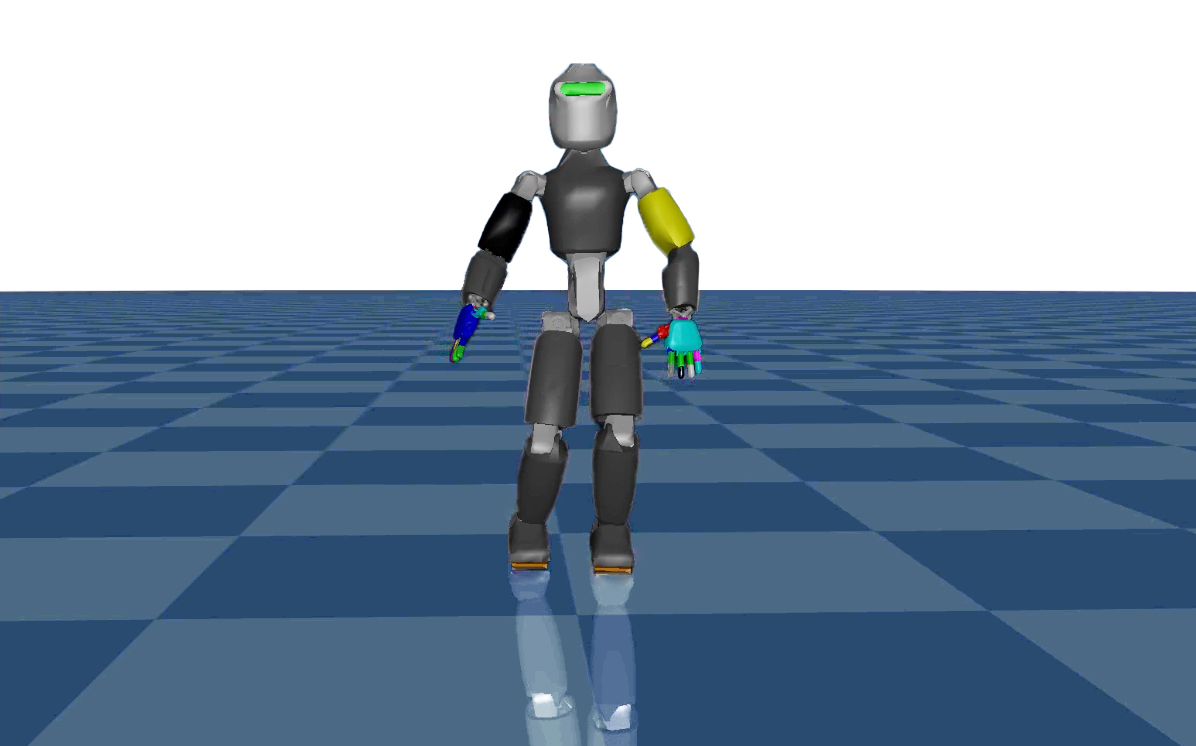
\includegraphics[width=0.7\textwidth]{Images/mujoco_ergocub.png}
\end{figure}

As robotics and reinforcement learning continue to merge and advance, with the increase of the environment and agent complexity, the computational cost of the simulation process increases as well, hence there's a growing demand for fast simulation environments that closely mimic real-world conditions. This is why these frameworks have a great impact on researchers, engineers, and developers to create and experiment with highly complex and realistic environments for training and testing \ac{RL} agents, essential for refining the control and decision-making capabilities of robots safely and efficiently. In the following sections, the physics simulators exploited in this work will be presented, highlighting their main features and limitations, with a focus on the implementation details of \jax, which is the core of the simulator used in the codesign loop.

\section{Nvidia ISAAC Gym}

\begin{figure}
    \centering
    \caption{NVIDIA Isaac Gym (CHANGE)}
    \label{fig:isaac_gym}
    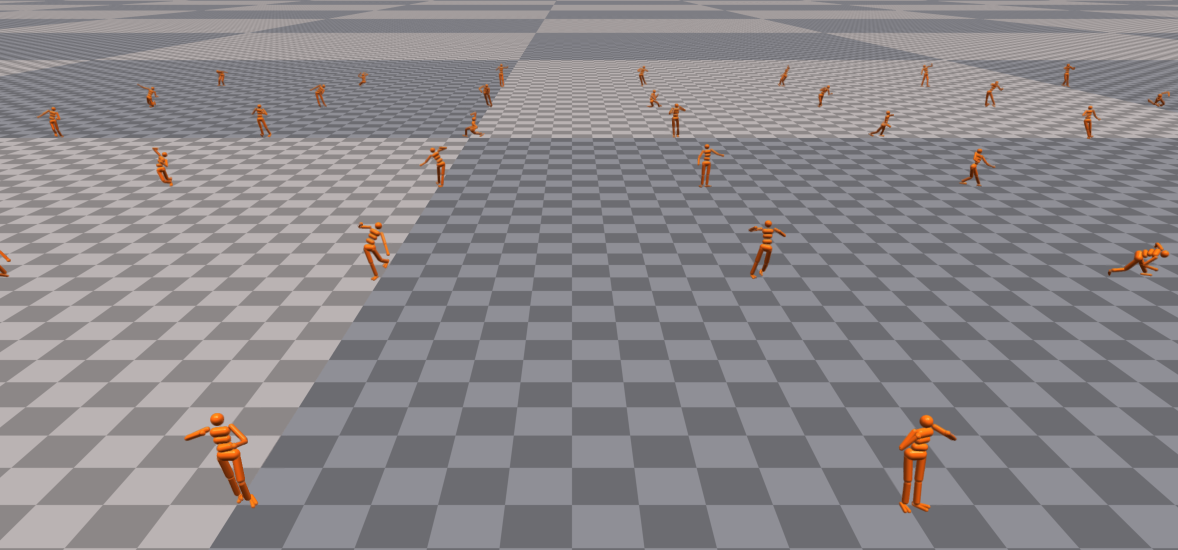
\includegraphics[width=0.7\textwidth]{Images/isaacgym_humanoid.png}
\end{figure}

In recent times, the use of \textit{Adversarial Motion Priors} \citep{peng_amp_2021} for reinforcement learning, which will be further discussed in \cref{chp:back_RLGA} has brought to the development of a new framework for physics simulation, called \textsc{isaac gym} \citep{makoviychuk_isaac_2021} which allows to simulate complex environments basing on \textsc{isaac sim} \citep{zhou_towards_2023}, a cyber-physical simulator that exploits NVIDIA PhysX and Omniverse, which offer a high-performance, cross-platform, real-time physics engine that allows to simulate rigid bodies in reduced coordinate articulations. \textsc{Isaac gym} then leverages the power of \texttt{rl\_games} \citep{rl-games2021} to completely work with \texttt{pytorch} \citep{paszke_pytorch_2019} tensors on \ac{GPU}s to accelerate the simulation process, allowing to train complex environments with multiple agents and objects.

The backend implementation of the simulator is written in \cpp while offering a frontend interface in Python, which allows us to easily build complex environments and agents, as well as to visualize the simulation process. Nevertheless, being the framework completely closed-source, it is not possible to extend the functionalities of the simulator, which is limited to the ones provided by the original developers.

\section{JAX: High-Performance Array Computing}

\begin{figure}[h]
    \centering
    \caption{JAX Overview}
    \label{fig:jax_logo}
    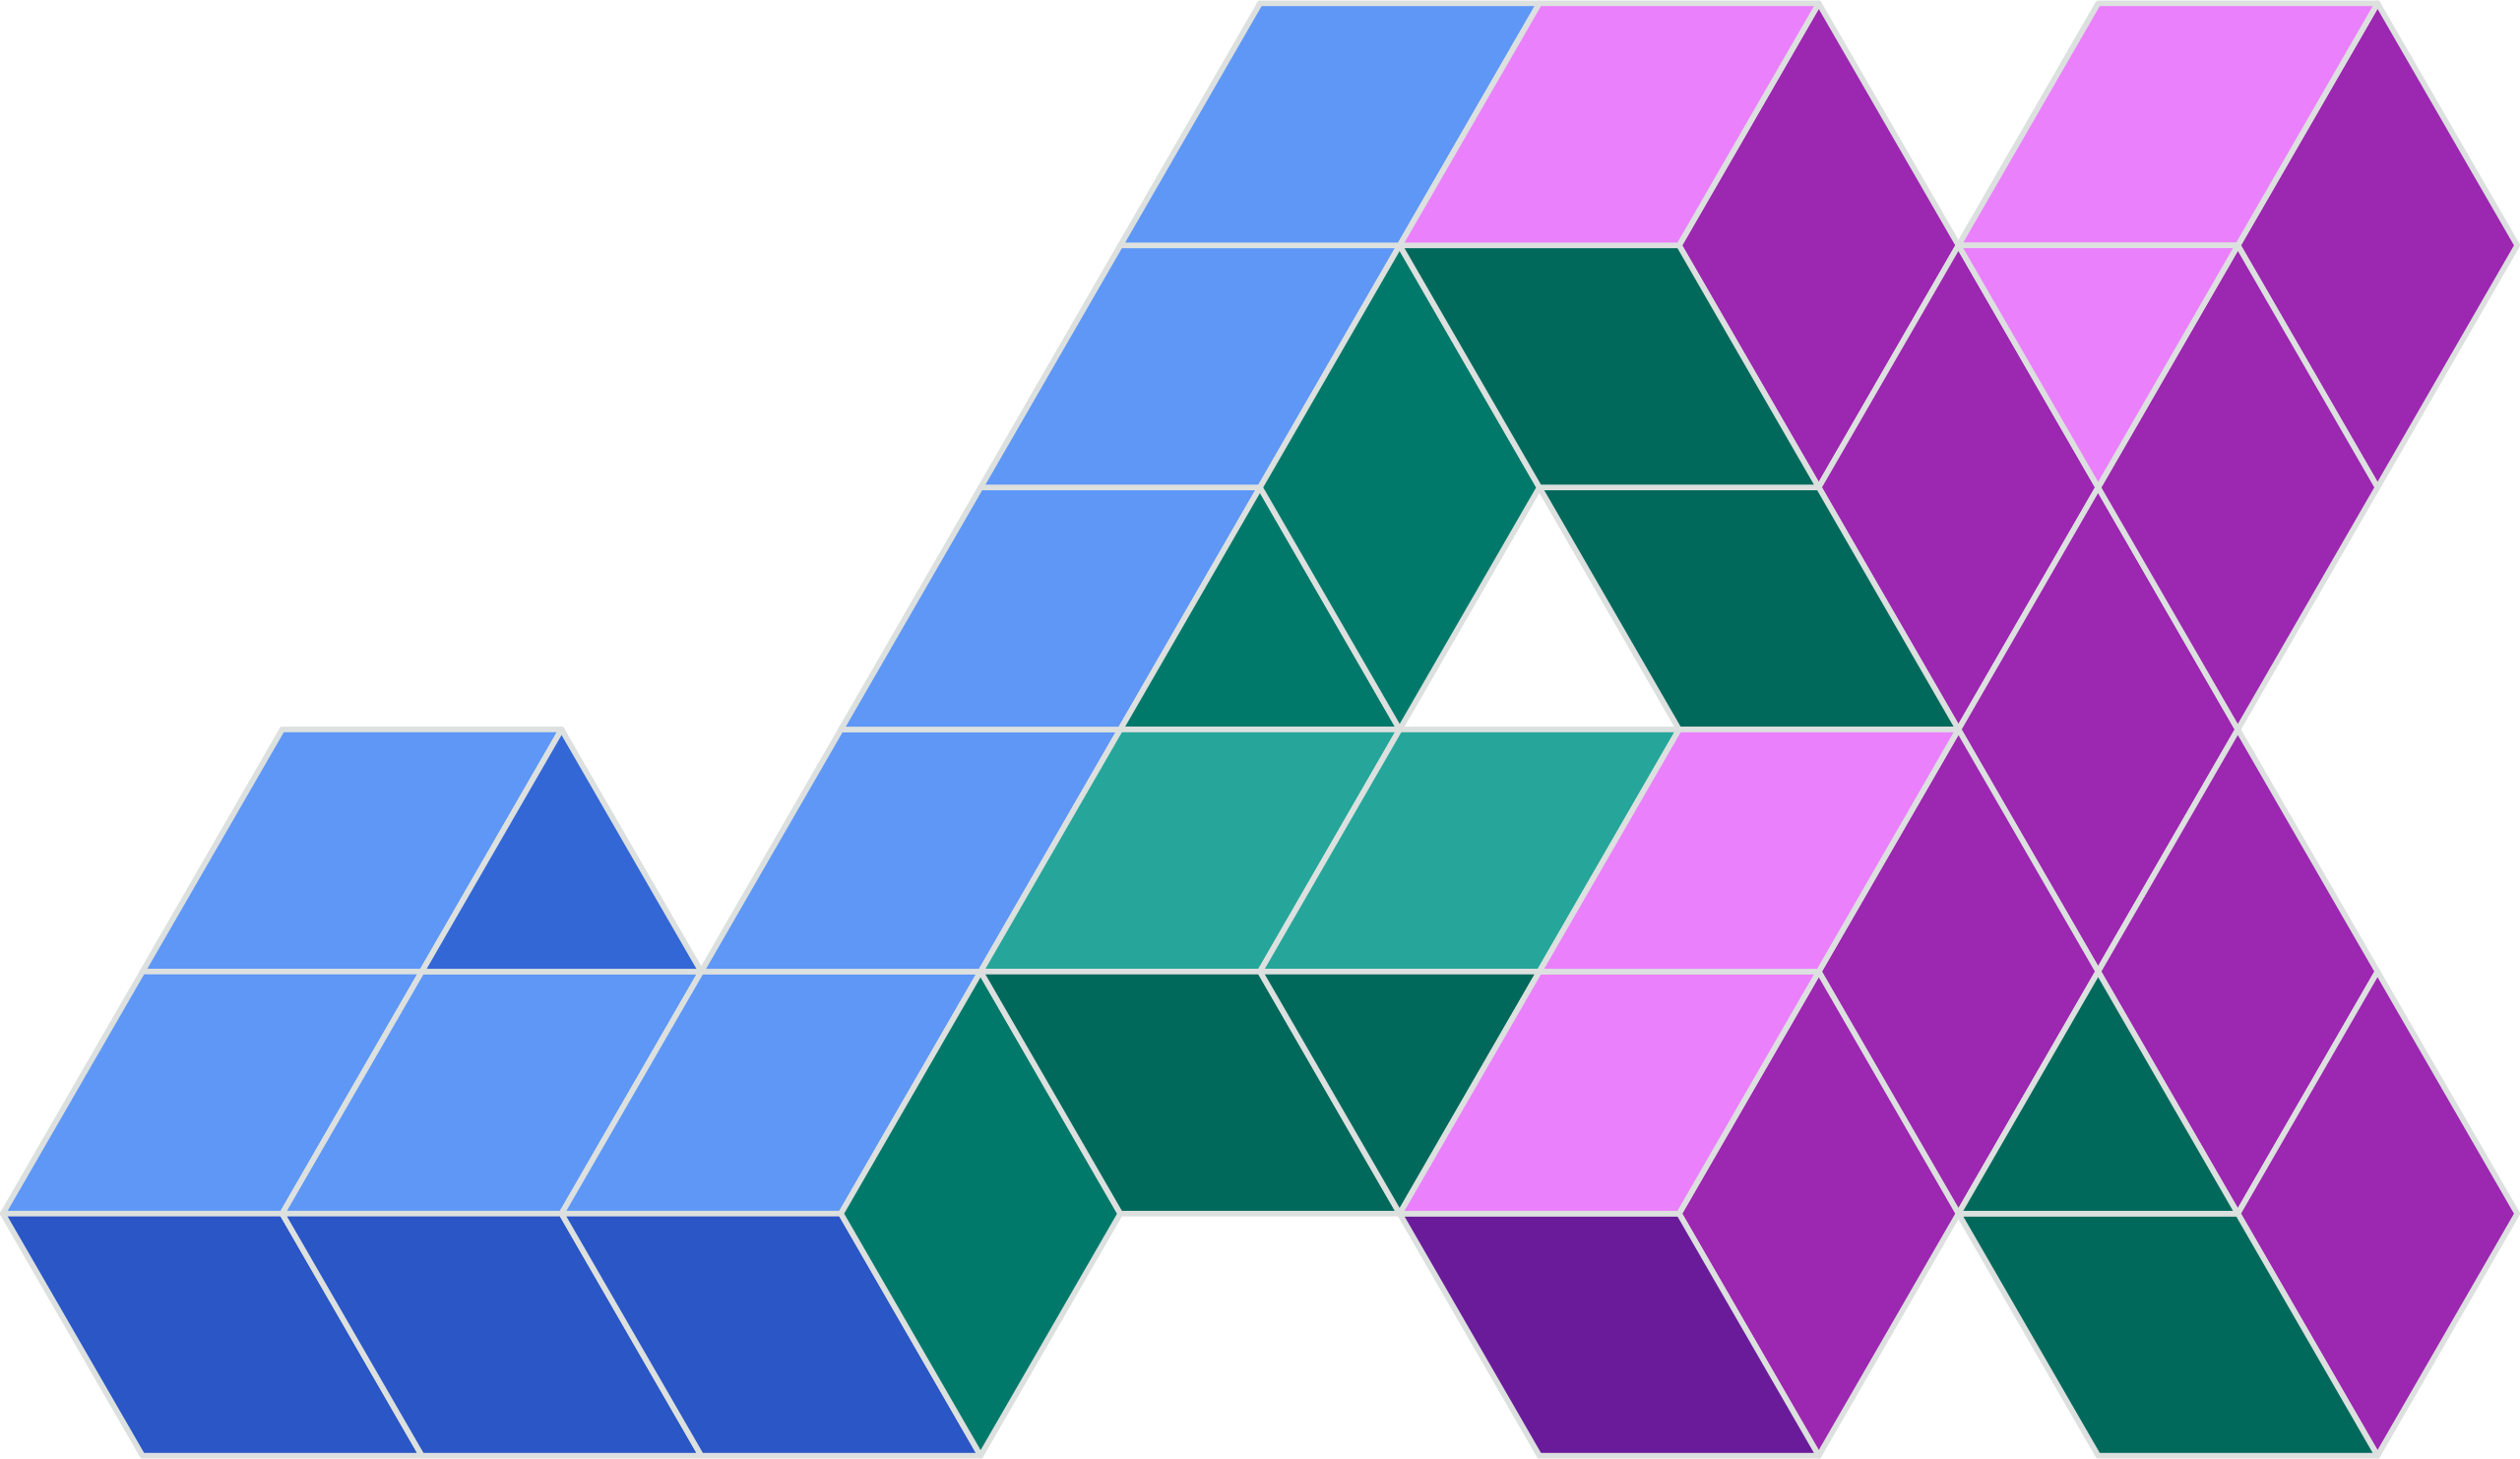
\includegraphics[width=0.3\textwidth]{Images/jax_logo.png} \qquad \qquad
    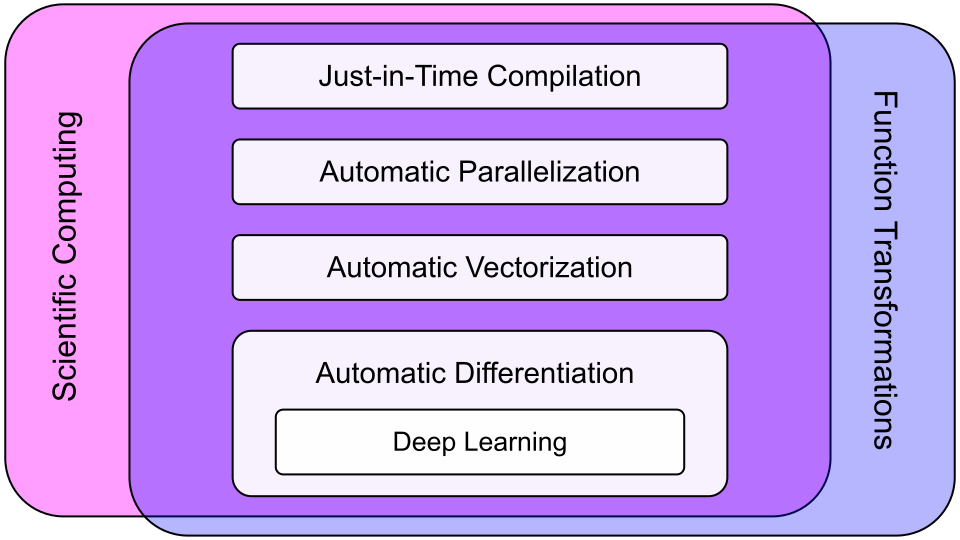
\includegraphics[width=0.4\textwidth]{Images/JAX-overview.png}
\end{figure}

Amongst the variety of framework that offers a high-level interface to make it easier for the user to write code that can be run on \ac{GPU}s, \jax \footnote{\url{https://github.com/google/jax}} \citep{bradbury_jax_2018,47008} is rapidly becoming one of the most popular choices. It exploits the power of \ac{XLA} \citep{50530}, which is a domain-specific, \textit{Just-In-Time} (\ac{JIT}), graph-based compiler for linear algebra that leverages efficient kernel fusion and lazy tensor materialization, firstly developed for TensorFlow \citep{tensorflow2015-whitepaper} and then extended to PyTorch and \jax itself.
Computations on \textit{Central Processing Units} (\ac{CPU}) also benefit from the use of \ac{JIT} compilation, which allows to compile the code at runtime and fused operations \citep{wang_kernel_2010,snider_operator_2023}, which allows combining multiple algebraic operations into a single \textit{Fused Multiply-Add} operation(\ac{FMA}), hence reducing the overhead of the compilation process and avoiding intermediate results by rounding the result of the multiplication to the nearest representable number in the given precision.
Moreover, \jax supports back and forward \textit{Automatic Differentiation} (\ac{AD}), which is a key feature for the implementation of deep learning algorithms, physical system modeling, and optimization.

A fresh and interesting alternative to \jax, that allows one to easily write \ac{GPU}-accelerated Python code is NVIDIA Warp \citep{warp2022}, which uses a kernel-based programming model that triggers \ac{JIT} compilation of Python code into \textit{Parallel Thread Execution} (\ac{PTX}) as an intermediate representation, which is then transformed into \textit{CUDA} code. With Omniverse integration, as a key feature, it supports the simulation of mesh grids, cloths, particles, and fluids, as well as the simulation of rigid bodies. Nevertheless, it is still in its early stages of development and it is not yet widely used in robotics research.


\subsection{JAX Implementation Details}

\jax uses a set of low-level primitives to support high-level array operations, which have the characteristic to be differentiable and \ac{JIT} compilable. What happens under the hood is that the Python callable gets traced, generating an \textit{Intermediate Representation} (\jax IR) which is a functional representation of the program. The \jax transformations like \texttt{vmap} and \texttt{grad} that allow vectorizing and differentiate the function, are then applied to the \jax IR, which is finally lowered to \ac{XLA} operations, ready to be executed on \ac{GPU} or \ac{TPU} devices.


\begin{figure}
    \centering
    \caption{JAX Tracing and Compilation Process}
    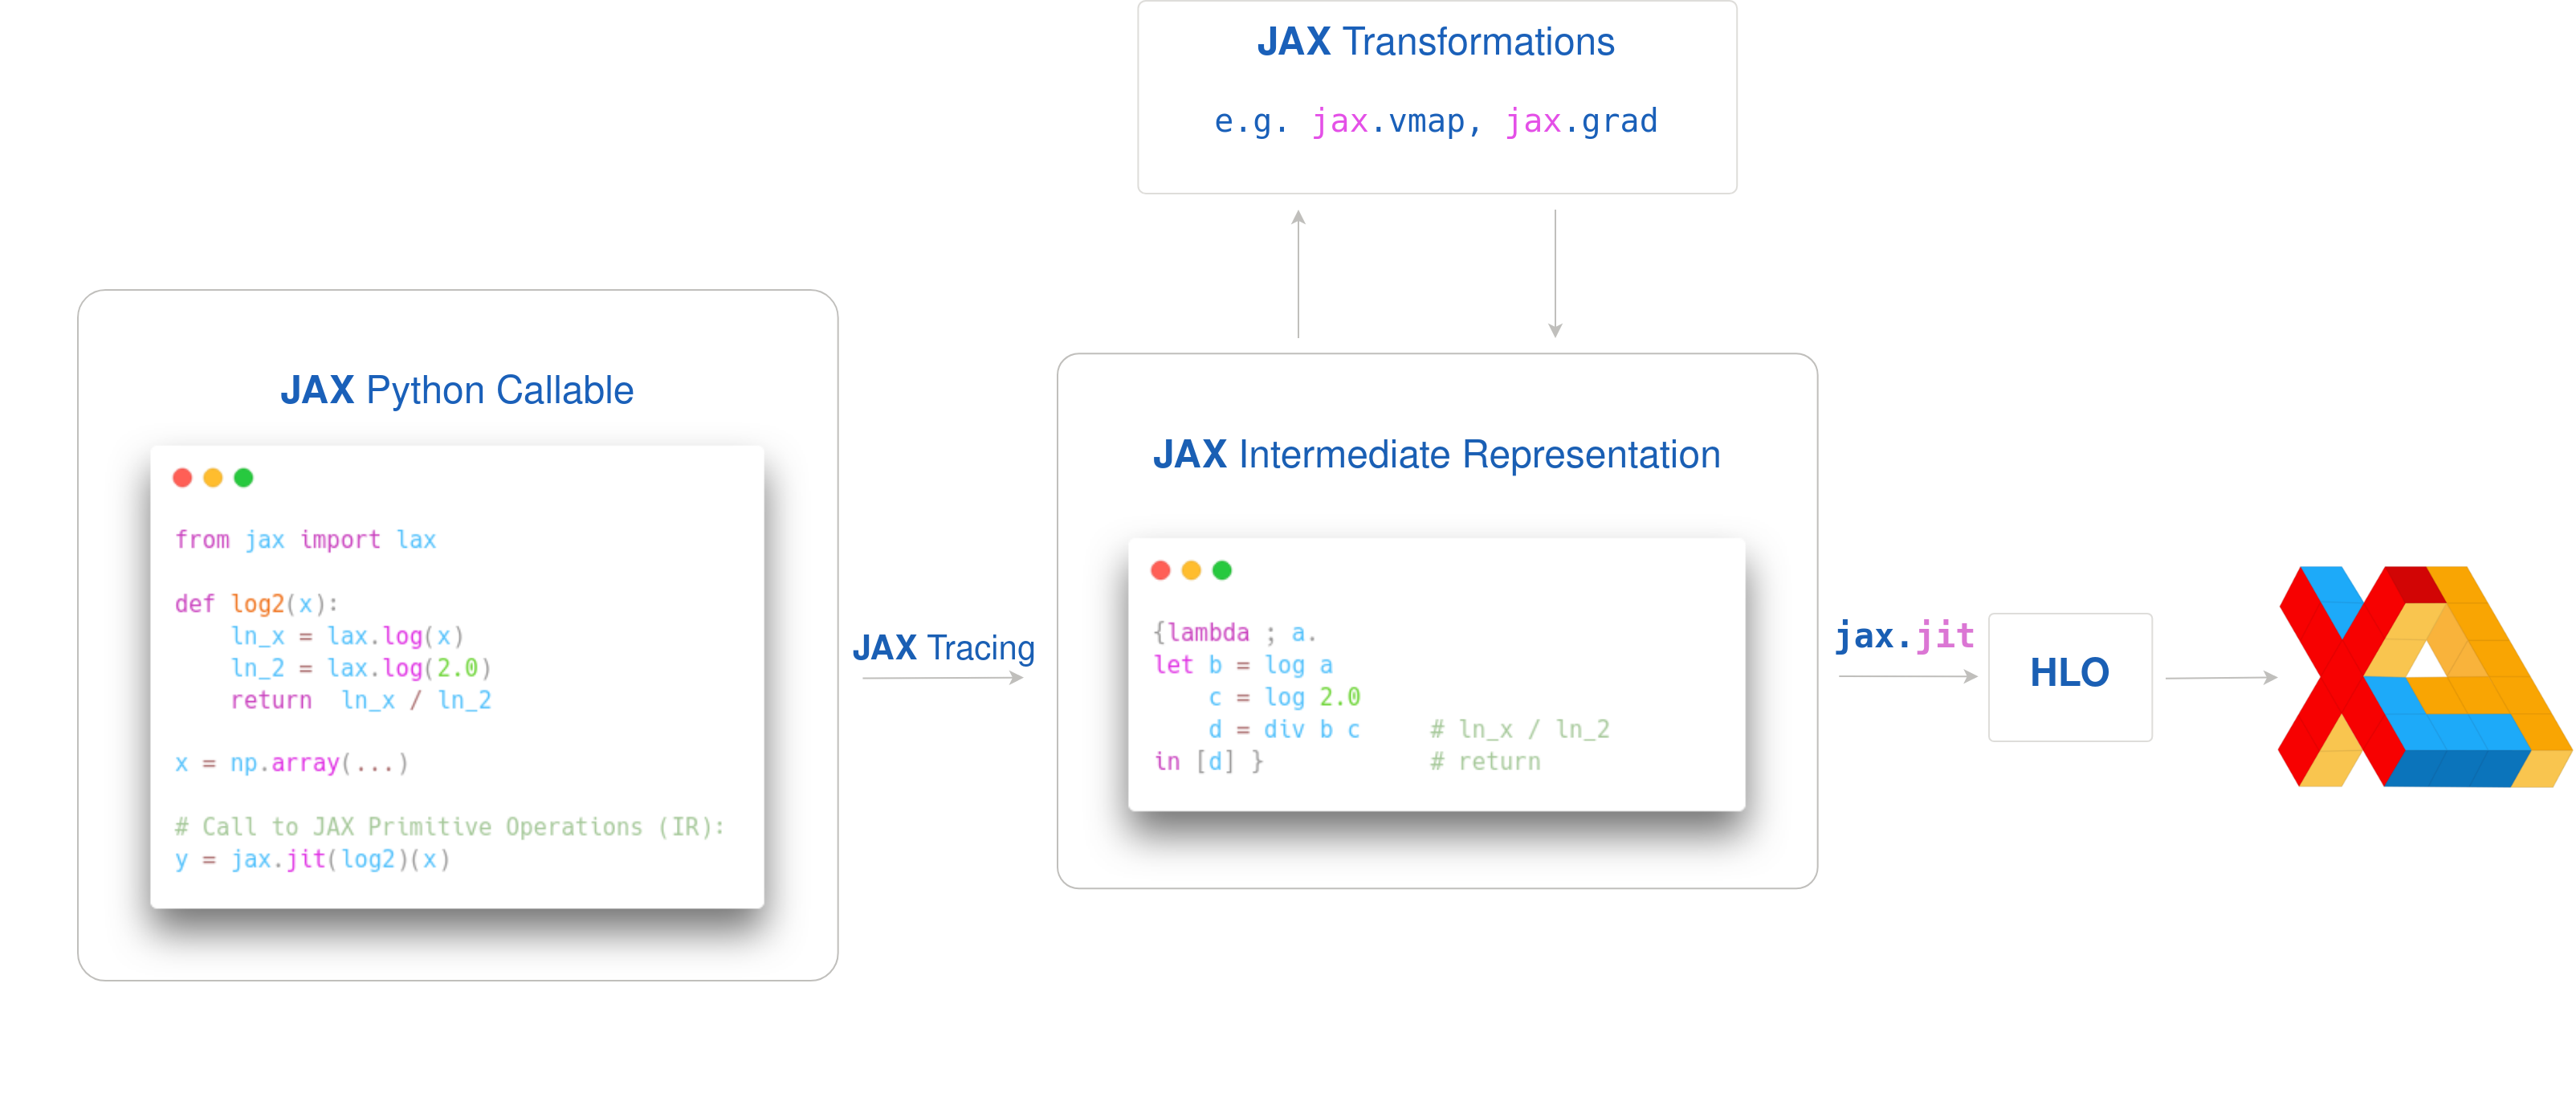
\includegraphics[width=\textwidth]{Images/jax_compute_graph_short.png}
\end{figure}

Creating \jax code requires following a set of rules, which ensures that the code can be compiled and potentially auto-differentiated. In fact, \ac{JIT} compilation requires the code to be static, i.e. the operations inside the function must not change between calls.
For example, the usage of \texttt{for}-loops and \texttt{if}-statements is not so straightforward, as the former involves dynamic iteration, which can disrupt the static nature of the code and will get unrolled during the compilation process, leading to a potentially huge computation graph causing memory issues, long compilation times and the impossibility to be forward and backward differentiated. The latter instead introduces conditional branches in the computation graph which cannot be managed by the \ac{XLA} compiler in a static way at runtime. Nevertheless, \jax offers a set of functions that allows to perform static iteration and conditional branching while being forward and backward differentiable and automatically compiled in \textit{Just-In-Time}, which are \texttt{jax.lax.scan} and \texttt{jax.lax.cond} respectively. Similarly, \texttt{while}-loops are not supported, but they can be implemented using \texttt{jax.lax.scan}, in which the termination condition is checked at each iteration, and when it is met, the loop is not stopped, but the iteration simply does not update the state, ensuring that the number of iterations is static and known at compile time.

\begin{figure}[h]
    \centering
    \caption{JAX vs Native Python For Loop}
    \label{fig:jax_python_forloop}
    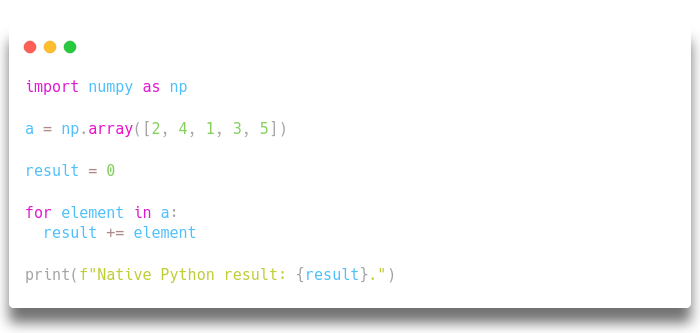
\includegraphics[width=0.45\textwidth]{Images/python_forloop.png}
    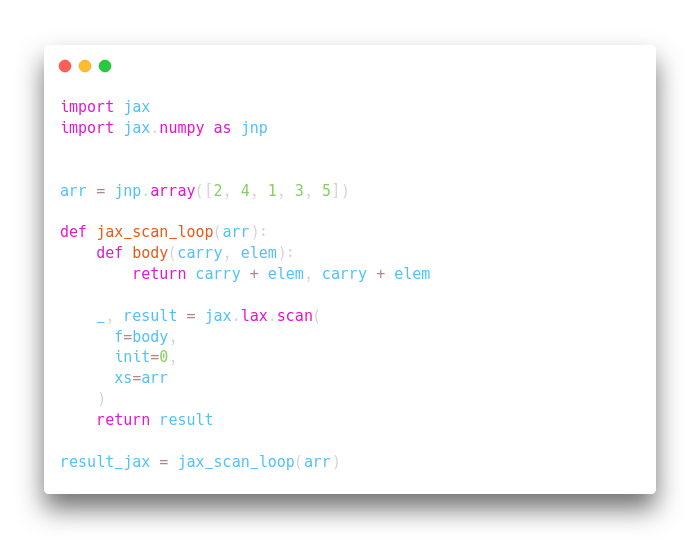
\includegraphics[width=0.45\textwidth]{Images/jax_forloop.png}
\end{figure}

Using \texttt{jax.lax.scan} and \texttt{jax.lax.cond} requires writing the code in a functional programming style, which is not always the most immediate choice for the user. In the examples reported in \cref{fig:jax_python_forloop}, a \texttt{body} function will get executed at each iteration which will have an initial value for the variable \texttt{carry} of \texttt{0} and will iterate through \texttt{arr}. The \texttt{cond} function will instead execute the \texttt{true\_fun} function if the condition \texttt{cond} is met, otherwise, it will execute the \texttt{false\_fun} function, as reported in \cref{fig:jax_python_if}. Note that with respect to the Python implementation, the \jax implementation requires declaring the type of the variable \texttt{x} as a \texttt{jax.numpy.ndarray}, this will ensure the creation of a \textit{PyTree} object.

\begin{figure}[h]
    \centering
    \caption{JAX vs Native Python If Statement}
    \label{fig:jax_python_if}
    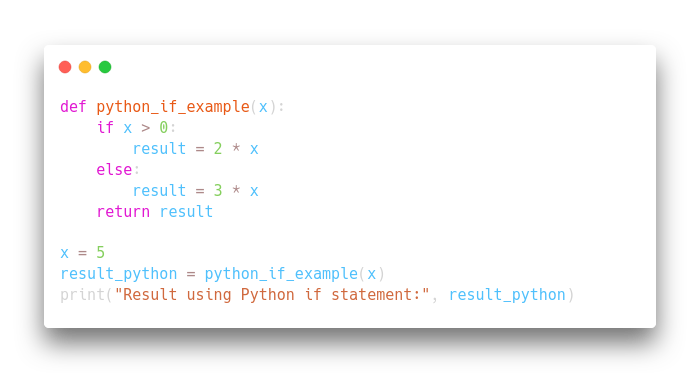
\includegraphics[width=0.49\textwidth]{Images/python_if.png}
    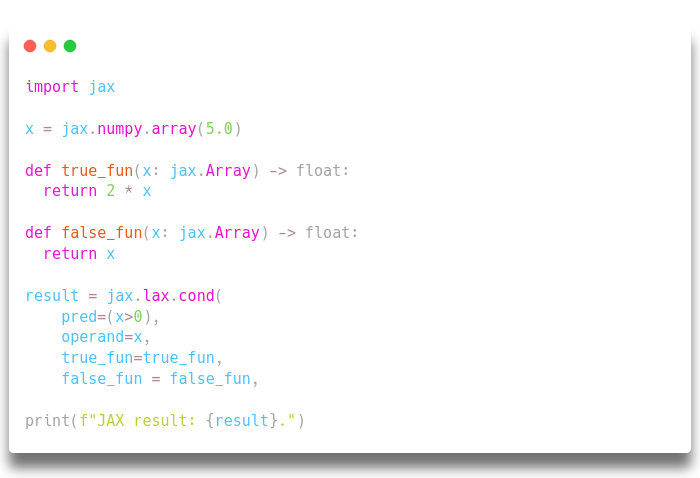
\includegraphics[width=0.49\textwidth]{Images/jax_if.png}
\end{figure}

Furthermore, \jax introduces a new optimized structure for fast and efficient computations on \ac{GPU}s, called \textit{PyTree}s, which is an object with a tree-like structure that can be used to represent nested data structures. The main advantage of using \textit{PyTree}s is that they can be used to represent and perform operations on heterogeneous data structures. In the example shown in \cref{fig:pytree_example} in fact, the \texttt{pytree} variable is an object containing four different data structures, thus being the \textit{leaves}, i.e. the outermost elements of the tree, compatible among each other, by calling \texttt{jax.tree\_map} on the \texttt{pytree} object, the function \texttt{x+1} can be applied to each leaf of the tree, returning a new \textit{PyTree} object with the same structure of the original one, but with the leaves modified by the function.

\begin{figure}[h]
    \centering
    \caption{Example Operation on a JAX PyTree}
    \label{fig:pytree_example}
    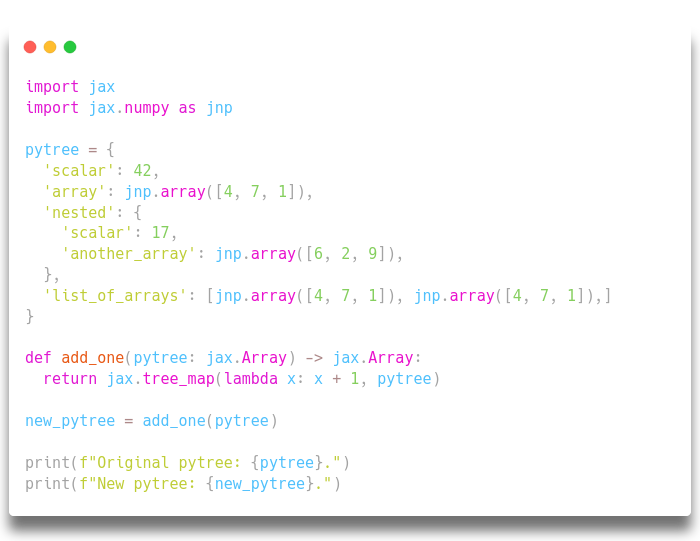
\includegraphics[width=\textwidth]{Images/pytree_example.png}
\end{figure}

\section{JAXSim}

It is immediate to think of the possibility of combining the power of \jax with the flexibility and ease of use of Python to create a physics simulator that can be easily extended and customized. This was the main idea behind \texttt{brax} \footnote{\url{https://github.com/google/brax}} \citep{freeman_brax_2021}, a differentiable rigid body physics simulator in maximal coordinates. Nevertheless, the absence of a high-level interface to immediately get the mechanical system quantities of the Euler-Poincare equation, as well as the lack of support for \ac{SDF} files, often used in model-based robotics research, led to the development of \jaxsim \footnote{\url{https://github.com/ami-iit/jaxsim}} \citep{ferigo_jaxsim_2022}, a hardware-accelerated physics simulator that exploits the strong parallelization capabilities and the \ac{JIT} compilation of \jax to speed up the simulation process.

Although being functional programming preferable in \jax, \jaxsim makes use of \textit{Object Oriented Programming} (\ac{OOP}) in order to create a modular and extensible framework easily accessible to the user. At this scope, the static nature of the objects is ensured throughout the simulator by using frozen \texttt{dataclasses}, which are immutable objects that cannot be modified after their initialization unless their mutability gets explicitly set, thus ensuring that the \textit{PyTree} structure of the objects is preserved when performing operations on them via the usage of context managers.

The use of \ac{OOP} is exploited in this work in order to add a layer of abstraction to the simulator, which allows to easily simulate the dynamics of motors inside the joints of a robotic system while maintaining the same interface of the original \jaxsim framework.


\section{Impacts and Contacts}
\label{sec:back_contacts}

When dealing with rigid body dynamics, the most common approach to model the contact between two bodies is to use a \textit{penalty-based} approach \citep{inproceedings}, which consists of adding a force to the system when the distance between two bodies is below a certain threshold. This approach is computationally efficient and easy to implement, but it does not allow to model the dynamics of the contact, which is often the case when dealing with high-velocity impacts. In fact, in the case of a high-velocity impact, the contact between two bodies is not perfectly inelastic, hence the partial elasticities of the materials involved in the collision induce vibrational modes in the system. This is why a \textit{compliant} approach is often preferred, which allows to model the dynamics of the contact, but it is computationally more expensive and requires a more complex implementation.

\subsection{Smooth Impacts}

In a high incident velocity impact between two solids, due to the nonperfect inelasticity, some of the kinetic energy is transferred to the vibrational model.

Considering a point particle with mass $m$ and position $\mathbf{q}(t): \mathbb{R} \rightarrow \mathbb{R}$ in a one-dimensional space, compliant with a spring with stiffness $k$ and a damper with damping coefficient $c$, the resulting force generated can be defined as:

\begin{equation}
    F = \begin{cases}
        -k\mathbf{q} - c\dot{\mathbf{q}} & \text{if } \mathbf{q} > 0    \\
        0                                & \text{if } \mathbf{q} \leq 0
    \end{cases}
\end{equation}

Considering an initial position $\mathbf{q}(t=0) = 0$ and a starting velocity $v_0 \in \mathbb{R}$ such that $\dot{\mathbf{q}}(t=0) = v_0 > 0$, i.e. the particle starts at the origin but moves towards the penetration region, will result in an active force $F(t) = -k\mathbf{q}(t) - c\dot{\mathbf{q}}(t)$ that will be applied to the particle until it reaches the equilibrium position $\mathbf{q} = 0$. The resulting motion will be a damped oscillation that can be derived from the Lagrangian mechanics as seen in \cref{eqn:lagrangian}, where the Lagrangian $\mathcal{L}$ of the system is defined as:

\begin{equation}
    \mathcal{L} = \mathcal{T} - \mathcal{V} = \frac{1}{2}m\dot{\mathbf{q}}^2 - \frac{1}{2}k\mathbf{q}^2
\end{equation}

which yields the following equation of motion:

\begin{equation}
    \ddot{\mathbf{q}} + \underbrace{\frac{c}{m}} _{\omega ^2} \dot{\mathbf{q}} + \underbrace{\frac{k}{m}} _\gamma \mathbf{q} = 0 \quad \rightarrow \quad \ddot{\mathbf{q}} + 2\zeta \omega \dot{\mathbf{q}} + \omega ^2 \mathbf{q} = 0
\end{equation}

where $\omega$ is the natural frequency of the system and $\gamma$ can be used to declare the damping ratio $\zeta = \frac{\gamma}{2\omega}$.

The solution of the resulting equation is the one of a first-order linear \ac{ODE}:

\begin{equation}
    \mathbf{q}(t) = \mathbf{q}_0 e^{-\zeta \omega t} \cos(\omega \sqrt{1 - \zeta ^2} t)
\end{equation}

which implies an oscillatory regime for $\zeta < 1$ and an exponential decay for $\zeta > 1$, also called overdamped regime.
Although relatively simple to implement, this approach is not always the most efficient, as it requires solving a \textit{differential algebraic equation} at each time step, which can be computationally expensive, making it extremely sensitive to the choice of the time step $h$.

\subsection{Non-smooth Impacts}

Considering two bodies and given points $p ^{(0)}$ fixed on body 0 and $p ^{(1)}$ fixed on body 1, the \textit{signed} distance between the two should be non-negative i.e. $c(p ^{(0)}, p ^{(1)}) \geq 0$, in order to avoid comprenetration.

The impact involves forces that change rapidly to cause jump discontinuities in the velocities $\dot{q}$. Therefore it is possible to state that the velocity before and after the impact at time $t_i$ differ:

\begin{equation}
    \lim _{t \uparrow t _i} \dot{q} = \dot{q} _{-} \neq \dot{q} _{+} = \lim _{t \downarrow t _i} \dot{q}
\end{equation}

Mathematically, the position $q(t)$ remains continuous while the velocity $\dot{q}(t)$ exhibits jump discontinuities, hence the acceleration $\ddot{q}(t)$ is not defined at impact times.

Considering the case of a spherical rigid body impacting an infinite plane, the convexity of the two objects implies that the closest point between the two can be identified uniquely. By writing the signed distance function with respect to the rigid body center of mass position $x(t)$, we get that $c(q(t)) = \tilde{c}(x(t)) \geq 0$, yet when the sphere is in contact with the plane we have that $\tilde{c}(x(t)) = 0$. With this approach, we can define two configuration manifolds: $Q _1 \subset \mathbb{R} ^2 \times \mathrm{SO}3$ for the planar motion and $Q _2 \subset \mathbb{R} ^3 \times \mathrm{SO}3$ for the spatial motion. Without loss of generality, the problem can be simplified in notation by defining a Lagrangian multiplier $\xi \in \mathbb{R}$ corresponding to the magnitude of the force acting in the normal direction at the contact point while keeping a configuration manifold $Q \in \mathbb{R}^3 \times \mathrm{SO}(3)$.
By using the augmented Lagrangian, the \cref{eqn:lagrangian} can be rewritten as:

\begin{equation}
    \frac{d}{dt} \frac{\partial}{\partial \dot{q}} \mathcal{L} - \frac{\partial}{\partial q} \mathcal{L} - J^\top \lambda = 0 \quad \text{and} \quad \varepsilon\lambda + g(q) = 0
\end{equation}

where $\lambda$ are the coordinates of $m$ one-dimensional point particles having position $\lambda _{j}$, $J$ is the Jacobian and  $g \in Q \times \mathbb{R} \rightarrow \mathbb{R} ^m$ is the configuration coordinate function, and by discretizing the time with a fixed time step $h$, we get:

\begin{equation}
    \int _0 ^h ds\xi^\top c(q(s)) \sim h\xi_0 ^\top c_0
\end{equation}

as the least action principle requires the discrete action to be minimized over the allowed trajectories $c(q_k) >0$, using the theorem of Karush-Kuhn-Tucker, we get to a stationarity condition that does not allow for energy conservation \citep{lacoursiere_ghosts_2007}.

\subsection{Approximate Impulse Model}

In a discrete mechanics framework, defining $h$ the fixed time step for all steps, if the violation in the impact point at step $i$ called $q _i$ is not too big, a good approximation of the incident velocity is:

\begin{equation}
    \dot{q} _{-} = \frac{q _i - q _{i-1}}{h}
\end{equation}

To estimate the outbound velocity $\dot{q} _{+}$ instead, we impose the discrete impulsive Newton impact law in one spatial dimension as:

\begin{equation}
    \dot{q} _{+} = -\psi \dot{q} _{-}
\end{equation}

where $\psi \in [0,1]$ is the \textit{restitution coefficient}.

A perfectly elastic collision corresponds to $\psi = 1$ in which the outbound velocity is the reflection of the incoming one. Now, given that the impulse occurs at a fixed position $q$, the only change in energy is a kinetic energy change, hence for the Newton-Poisson impact law for a point particle of mass $m$ with kinetic energy $\mathcal{T}(q, \dot{q})$, the change in energy is:

\begin{equation}
    E _{+} - E _{-} = \mathcal{T}(q, \dot{q} _{+}) - \mathcal{T}(q, \dot{q} _{-}) = (\psi ^2 - 1) \mathcal{T}(q, \dot{q} _{-}) \leq 0
\end{equation}

To generalize in three dimensions, we define an estimate of the normal component of the incident velocity with respect to the contact manifold as $C _k \dot{q} _{-}$ where $C _k$ is the $n _c \times n$ Jacobian matrix of the $n _c$ contact surface evaluated at the discrete time $k$. Using the complementarity formulation, assuming the presence of other inequality constraints with the agglomerated Jacobian $J$, adding regularization parameters with diagonal non-negative matrices $\Sigma$ and $\Xi$, and considering the diagonal matrix for restitution coefficients $\Psi = \text{diag}(\psi _1, \psi _2, \dots, \psi _{n _c}),  \psi _i \in [0, 1]$, we get the following linear complementarity problem (LCP):

\begin{equation}
    \begin{rcases}
        M\dot{q} _{+} - G ^\top _k \lambda - C ^\top _k \dot{q} & = M \dot{q} _{-}    \\
        G _k \dot{q} _{+} + \Sigma \lambda                      & = G _k \dot{q} _{-} \\
        C _k \dot{q} _{+} + \Psi C \dot{q} _{-} + \Xi \dot{q}   & = w                 \\
    \end{rcases} \quad \text{subject to
        :  } \quad \dot{q} \geq 0 \perp w \geq 0
\end{equation}

By solving the optimization above, it can be shown that this leads to $T _{+} \leq T _{-}$, therefore the impulsive stage can only decrease the kinetic energy.

\chapter{Reinforcement Learning and Genetic Algorithms}
\label{chp:back_RLGA}

This chapter presents the minimal theoretical background of reinforcement learning and genetic algorithms. A particular focus is given to the \ac{PPO} algorithm, which is the main algorithm used in the \ac{RL} framework of the codesign process. Finally, some novel approaches in the field of \ac{RL} are presented. This chapter are based on the work of \citet{sutton_reinforcement_1998,li_deep_2018,agarwal_deep_2022}

\section{Fundamentals of Reinforcement Learning}

Reinforcement learning comes from a fusion of optimal control theory and the theory of machine learning and consists of guiding agents in dynamic environments to maximize cumulative rewards. Unlike supervised learning, \ac{RL} doesn't require labeled input/output pairs, and it focuses on striking a balance between exploring uncharted territory and exploiting existing knowledge. The environment is often modeled as a Markov decision process, distinguishing it from classical dynamic programming by its ability to handle large \ac{MDP}s without assuming an exact mathematical model.

Reinforcement learning's versatility extends to a wide range of disciplines like game theory, control theory, and swarm intelligence. Contrary to optimal control theory's emphasis on exact solutions, \ac{RL} addresses problems without a known mathematical model. Assessing an agent's performance against an optimally acting agent introduces the concept of regret, a measure from decision theory of the disparity between what the agent achieves and the best possible outcome, prompting a deeper understanding of the effectiveness and improvement potential within the learning process. For that, \ac{RL} excels in scenarios involving a trade-off between long-term and short-term rewards, requiring agents to consider the extended consequences of their actions. Overall, its adaptability makes it a powerful tool for complex problems that are difficult to model mathematically, such as multibody dynamics.

\begin{figure}
    \centering
    \caption{Reinforcement Learning Framework}
    \label{fig:rlframework}
    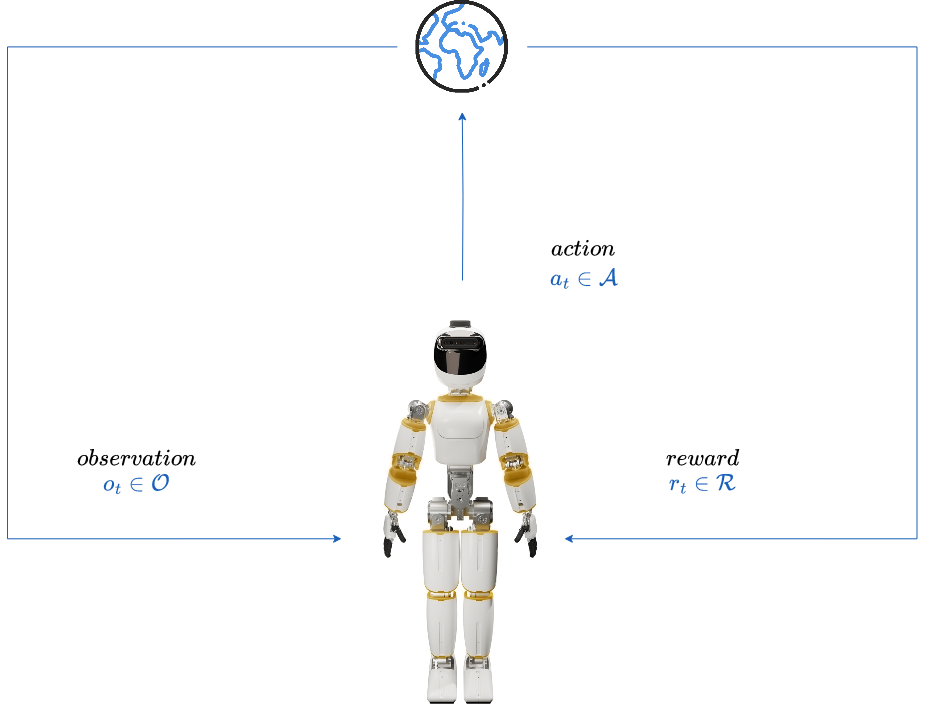
\includegraphics[width=.7\textwidth]{Images/rl_ergocub.png}
\end{figure}

\subsection{Key Mathematics}

\paragraph{Markov Decision Process} A \ac{MDP} is defined as a five-tuple $\mathcal{M} = (\mathcal{S}, \mathcal{A}, \mathcal{F}, r, \gamma)$ where:

\begin{itemize}
    \item $\mathcal{S}$ is the set of environment states $\mathbf{s} \in \mathcal{S}$, which may be either discrete or continuous
    \item $\mathcal{A}$ is the set of agent actions $\mathbf{a} \in \mathcal{A}$ which in a similar fashion may be continuous or discrete
    \item $\mathcal{F} (\mathbf{s}^\prime | \mathbf{s}, \mathbf{a}): \mathcal{S} \times \mathcal{A} \times \mathcal{S} \rightarrow \mathcal{S}$ is the state-transition function space that describes a conditional probability distribution $\mathcal{F}(\mathbf{s} _{t+1}|\mathbf{s}_t, \mathbf{a} _t)$ that describes the dynamics of the system
    \item $\mathcal{R} (\mathbf{s}^\prime, \mathbf{a}, \mathbf{s}): \mathcal{S} \times \mathcal{A} \times \mathcal{S} \rightarrow \mathbb{R}$ is the reward function
    \item $\gamma \in [0,1]$ is the discount factor that determines the weight of future rewards
\end{itemize}

If the environment is \textit{deterministic}, state transitions can be expressed with a state-transition function $\mathcal{F}: \mathcal{S} \times \mathcal{A} \times \mathcal{S} \rightarrow \mathcal{S}$, if the environment is \textit{stochastic}, state transitions can be expressed with the \textit{state-transition probability density function}, i.e. $\mathcal{F}: \mathcal{S} \times \mathcal{A} \times \mathcal{S} \rightarrow \mathbb{P}[\mathcal{S}]$.

As a reinforcement learning scenario has no prior knowledge regarding the data used for training, the state-transition map and the reward function are unknown.


\paragraph{Kullback-Leibler Divergence} The \ac{KL} divergence is a measure of how one probability distribution is different from a second, reference probability distribution. In other words, the \ac{KL} divergence measures the expected number of extra bits required to code samples from one distribution, given that we are using a code based on the reference distribution. The \ac{KL} divergence is defined as:

\begin{equation}
    \mathrm{KL}(P||Q) = \mathbb{E} _{x \sim P} \left[ \log \frac{P(x)}{Q(x)} \right] \qquad \in \left[0, \infty \right]
\end{equation}

where $P$ and $Q$ are two probability distributions. The \ac{KL} divergence is not symmetric, i.e. $\mathrm{KL}(P||Q) \neq \mathrm{KL}(Q||P)$. In the framework of reinforcement learning, it is commonly used to have a measure of how much the policy has changed from the previous iteration, in order to avoid too large policy updates, therefore what is actually seeked is the minimization of the \textit{reverse} \ac{KL} divergence $\mathrm{KL}(Q||P)$. In fact, in this mode-seeking behavior, the convergence will be achieved when the policy is close enough to the optimal policy, which is the one that maximizes the expected reward, i.e. when the \ac{KL} divergence is zero.

\subsection{Core Principles of Reinforcement Learning}

In general, a reinforcement learning process can be described therefore as a \textit{partially observable Markov decision process}, in which the tuple describing the problem assumes the form $\mathcal{M} =  (\mathcal{S}, \mathcal{A}, \mathcal{O}, \mathcal{F}, r, \gamma)$, where the new variable $\mathcal{O}$ is defined as the observation space. For the purpose of this discussion and to simplify the notation, the training process will always be considered \textit{fully observable}, e.g. the observation space will be equal to the state space $\mathcal{O} = \mathcal{S}$.

At each time step $t$, the agent receives from the environment a state $\mathbf{s}_t \in \mathcal{S}$ and following a policy $\pi (\mathbf{a}_t | \mathbf{s}_t)$ outputs an action $\mathbf{a} \in \mathcal{A}$. The environment will, via a transition function $\mathcal{F}$ output a reward $r$ and an observation $\mathbf{o} \in \mathcal{O}$, yield an evolution of the state:

\begin{equation}
    \mathcal{F}(\mathbf{s} _{t+1}, r _{t+1} | \mathbf{s} _t, \mathbf{a} _t)
\end{equation}

in which $r_t \in \mathbb{R}$ is the reward at time $t$, or \textit{immediate reward}.
The reward function can be determined by the expected value of the immediate reward

\begin{equation}
    \label{eqn:reward_function}
    \mathcal{R}(\mathbf{s} _t, \mathbf{a} _t, \mathbf{s} _{t+1}) = \mathbb{E} \left[ r _t | \mathbf{s} _t, \mathbf{a} _t, \mathbf{s} _{t+1} \right] = \sum _t r _t \frac{\mathcal{F}(\mathbf{s} _{t+1}, r _{t+1} | \mathbf{s} _t, \mathbf{a} _t)}{\mathcal{F}(\mathbf{s} _{t+1} | \mathbf{s} _t, \mathbf{a} _t)}
\end{equation}

As the immediate reward depends on the state at time $t+1$, and therefore how action $\mathbf{a} _t$ affects the state at time $t$, we can define a \textit{return} $G _t$ as the total reward collected from time $t$ to the end of the episode:

\begin{equation}
    G _t = \sum ^{T - t} _{k = 0} r _{t+k+1}
\end{equation}

where $T$ is the final time step of the episode. As in continuous tasks the episode length is infinite, the return is usually defined as the discounted sum of rewards by introducing a discount factor $\gamma \in [0,1]$:

\begin{equation}
    \label{eqn:recursive_return}
    G _t = r_t + \gamma r _{t+1} + \gamma ^2 r _{t+2} + \dots = \sum ^{\infty} _{k = 0} \gamma ^k r _{t+k+1}
\end{equation}

From this definition, it is clear that when the discount factor is equal to $0$, the agent will only consider the immediate reward, while if it is equal to $1$, the agent will consider the total reward. In practice, the discount factor is usually set to a value close to $1$.

In \ac{DRL} the policy is described by a neural network, therefore it is modeled as a probability distribution parameterized by the set of the \ac{NN} weights and biases $\boldsymbol{\theta}$. In a standard \textit{Multi Layer Perceptron} policy, $\pi _{\boldsymbol{\theta}}(\mathbf{a} | \mathbf{s})$ is a multivariate Gaussian distribution with diagonal covariance matrix, i.e. $\pi _{\boldsymbol{\theta}}(\mathbf{a} | \mathbf{s}) = \mathcal{N}(\mu = \boldsymbol{\mu}(\mathbf{s}), \sigma = \boldsymbol{\sigma}(\mathbf{s}, \boldsymbol{\theta}))$, where $\mu$ and $\sigma$ are the mean and the standard deviation of the distribution, respectively. The policy is then defined as:

\begin{equation}
    \pi _{\boldsymbol{\theta}}(\mathbf{a} \mid \mathbf{s}) = \frac{1}{\sqrt{2 \pi \boldsymbol{\sigma} ^2}} \exp \left(- \frac{(\mathbf{a} - \boldsymbol{\mu}) ^2}{2 \boldsymbol{\sigma} ^2} \right)
\end{equation}

or, in terms of action space:

\begin{equation}
    a _t \sim \pi _{\boldsymbol{\theta}}(\cdot | s_t): \mathcal{S} \rightarrow \mathbb{P}(\mathcal{A})
\end{equation}

By defining the \textit{trajectory} generated by a policy $\pi$ a sequence of tuples state-action for a given episode of length $T$ as:

\begin{equation}
    h ^{\pi} = \left\{ (\mathbf{s} _0, \mathbf{a} _0), (\mathbf{s} _1, \mathbf{a} _1), \dots, (\mathbf{s} _{T-1}, \mathbf{a} _{T-1}), (\mathbf{s} _T) \right\}
\end{equation}

in which the initial state $\mathbf{s} _0$ gets sampled from the initial state distribution $p(\mathbf{s} _0)$.
In \textit{on-policy} method the policy is updated on the trajectory generated by the current policy, while in \textit{off-policy} methods the policy is updated on a trajectory generated by a different policy, therefore while on-policy methods like \ac{PPO} and \ac{TRPO} result in more stable training, off-policy methods like \ac{TD3} and \ac{SAC} are more sample efficient as they can sample from a \textit{replay buffer} of past trajectories.

Since the agent has no apriori knowledge on future rewards, it will try to learn a \textit{state-value function} $V _{\boldsymbol{\phi}}(\mathbf{s})$ that estimates the expected return from a given state $\mathbf{s}$, where $\boldsymbol{\phi}$ is the set of parameters of the value function:

\begin{equation}
    V _{\boldsymbol{\phi}}(\mathbf{s}) = \mathbb{E} _{h^{\pi}} \left[ G _t | \mathbf{s} _t = \mathbf{s} \right] = \mathbb{E} _{h^{\pi}} \left[ \sum ^{\infty} _{k = 0} \gamma ^k r _{t+k+1} | \mathbf{s} _t = \mathbf{s} \right]
\end{equation}

and will be then used to estimate the advantage of an action $\mathbf{a}$, e.g. a measure of how much an action can improve the expected return from a given state in the future.
If we define the \textit{action-value} function $Q _{\boldsymbol{\phi}}(\mathbf{s}, \mathbf{a})$ as the expected return from a given state $\mathbf{s}$ and action $\mathbf{a}$:

\begin{equation}
    Q (\mathbf{s}, \mathbf{a}) = \mathbb{E} _{h^{\pi}} \left[ G _t | \mathbf{s} _t = \mathbf{s}, \mathbf{a} _t = \mathbf{a} \right] = \mathbb{E} _{h^{\pi}} \left[ \sum ^{\infty} _{k = 0} \gamma ^k r _{t+k+1} | \mathbf{s} _t = \mathbf{s}, \mathbf{a} _t = \mathbf{a} \right]
\end{equation}

then the advantage function can be defined as the difference between the action-value function and the state-value function, i.e. if an action $\mathbf{a}$ induces a state $\mathbf{s}$ producing a greater expected return, then the advantage will be negative, otherwise it will be positive:

\begin{equation}
    A (\mathbf{s}, \mathbf{a}) = Q (\mathbf{s}, \mathbf{a}) - V (\mathbf{s})
\end{equation}

Since the state-value function represents the expected return from a given state, it can be interpreted as a measure of how good a policy is, therefore the optimal policy $\pi ^*$ is the one that maximizes the state-value function. Similarly, the optimal action-value function $Q ^*$ is the one that maximizes the expected return from a given state-action pair:

\begin{equation}
    \pi ^* = \underset{\pi}{\arg\max} \ V (\mathbf{s}) \qquad Q ^* = \underset{\pi}{\arg\max} \ Q (\mathbf{s}, \mathbf{a})
\end{equation}

Recalling the recursive definition of the return presented in \cref{eqn:recursive_return} and the reward function definition in \cref{eqn:reward_function}, we can define the \textit{Bellman equation} for the state-value function as:

\begin{flalign}
    V (\mathbf{s}) & = \mathbb{E} _{h^{\pi}} \left[ G _t \mid \mathbf{s} \right] = \mathbb{E} _{h^{\pi}} \left[ r _t + \gamma G _{t+1} \mid \mathbf{s} \right]                                                                                                                         \\
                   & = \sum _{\mathbf{a}} \pi(\mathbf{a} \mid \mathbf{s})  \sum _{\mathbf{s} ^\prime \in \mathcal{S}} \mathcal{F}(\mathbf{s} ^\prime \mid \mathbf{s}) \left[\mathcal{R}(\mathbf{s} ^\prime, \mathbf{s}) + \gamma \mathbb{E} _{h^{\pi}} \right]  V (\mathbf{s} ^\prime)
\end{flalign}

and similarly for the action-value function:

\begin{flalign}
    Q (\mathbf{s}, \mathbf{a}) & = \mathbb{E} _{h^{\pi}} \left[ G_t \mid \mathbf{s}, \mathbf{a} \right]                                                                                                                                                                                                   \\
                               & = \mathbb{E} _{h^{\pi}} \left[ r _t + \gamma G_{t+1} \mid \mathbf{s}, \mathbf{a} \right]                                                                                                                                                                                 \\
                               & = \sum _{\mathbf{s} ^\prime \in \mathcal{S}} \mathcal{F}(\mathbf{s} ^\prime \mid \mathbf{s}, \mathbf{a}) \left[ \mathcal{R}(\mathbf{s} ^\prime, \mathbf{a}, \mathbf{s}) + \gamma \mathbb{E} _{h^{\pi}} \right] \left[ Q (\mathbf{s} ^\prime, \mathbf{a} ^\prime) \right]
\end{flalign}

\subsection{Policy Gradient Methods}

In continuous action spaces, as the optimal policy function $Q ^*(\mathbf{s}, \mathbf{a})$ is unknown, it is usually modeled as an optimized parametric function $\pi _{\theta}(\mathbf{a} | \mathbf{s})$ that outputs the probability of taking an action $\mathbf{a}$ in a state $\mathbf{s}$, where $\theta$ is the set of parameters of the policy. Therefrom, we can define a stochastic objective function $J(\theta)$ as the expected return of the policy $\pi _{\theta}$, being the return a random variable. Defining also the probability of a trajectory $h ^{\pi}$ as the probability of the initial state $s _0$ times the probability of the action $a _0$ times the probability of the next state $s _1$ and so on, e.g.

\begin{equation}
    \mathbb{P}(h ^{\pi}) = \mathbb{P}(s _0) \mathbb{P}(a _0 | s _0) \mathbb{P}(s _1 | s _0, a _0) \dots = \mathbb{P}(s _0) \prod ^{\infty} _{t = 0} \pi _{\theta} (a _t | s _t) \mathbb{P}(s _{t+1} | s _t, a _t)
\end{equation}

we can define the objective function as:

\begin{equation}
    J(\theta) = \mathbb{E} _{\pi _{\theta}} \left[ G _t \right] = \mathbb{E} _{\pi _{\theta}} \left[ \sum ^{\infty} _{k = 0} \gamma ^k r _{t+k+1} \right]
\end{equation}

from which we can derive the policy update rule once defined the policy gradient:

\begin{equation}
    \theta _{t+1} = \theta _t + \alpha \nabla _{\theta} J(\pi)
\end{equation}

where $\alpha \in \mathbb{R} ^+$ is the learning rate. The policy gradient is then defined as:

\begin{equation}
    \nabla _{\theta} J(\pi) = \nabla _{\theta} \int _{h ^{\pi}} \mathbb{P}(h ^{\pi})G(h ^{\pi})dh ^{\pi} = \dots = \mathbb{E} _{h^{\pi}} \left[ \sum ^{\infty} _{k = 0} \gamma ^k \nabla _{\theta} \log \pi _{\theta} (a _t | s _t) G _t \right]
\end{equation}

\subsubsection{Proximal Policy Optimization}

Amongst policy gradient methods, the \textit{Proximal Policy Optimization} (\ac{PPO}) is by far one of the most used and effective algorithms. It is a family of first-order methods that use a \textit{surrogate objective} in order to ensure a \textit{trust region} on the policy update.
Moreover, being an \textit{actor-critic} method, it uses two neural networks, one for learning the policy and one for learning the value function, acting as a feedback  loop for the policy network.

The version of \ac{PPO} adopted in this work uses a clipped surrogate objective and introduces a penalization term on the \ac{KL} divergence between the new and the old policy, ensuring small policy updates that would otherwise lead to unstable training, once defined:

\begin{equation}
    \mathfrak{R} _t (\boldsymbol{\theta}) = \frac{\pi_{\boldsymbol{\theta}} (\mathbf{a}_t \mid \mathbf{s}_t)}{\pi _{\boldsymbol{\theta}_{\text{old}}} (\mathbf{a}_t \mid \mathbf{s}_t)}
\end{equation}

resulting in the following formulation:

\begin{equation}
    \mathcal{L} (\boldsymbol{\theta}) = \hat{\mathbb{E}} \left[\min \left\{ \mathfrak{R}_t(\boldsymbol{\theta}) \hat{A}_t, \text{clip}\left(\mathfrak{R}_t(\boldsymbol{\theta}) , 1- \varepsilon, 1+\varepsilon \right)  \right\} - \beta \mathrm{KL} [\pi_{\boldsymbol{\theta}_{\text{old}}} (\cdot \mid \mathbf{s}_t), \pi_{\boldsymbol{\theta}} (\cdot \mid \mathbf{s}_t) ] \right]
\end{equation}

in which the $\text{clip}$ operator bounds the first argument in the interval $[1-\varepsilon, 1+\varepsilon]$, $\varepsilon$ is the clipping coefficient, $\hat{\mathbb{E}}$ is the empirical expectation, $\hat{A}_t$ is the advantage estimate at time $t$ and $\beta$ is the penalty coefficient for the KL divergence.


% The most common optimizer for \ac{NN} parameters is the first-order gradient-based optimization of stochastic objective function update ADAM \citep{kingma_adam_2017}, reported in \cref{alg:adam}, which
% updates exponential moving averages of the two gradients, where $\beta_1$ and $\beta_2$ control the decay rates of the moving averages, which are then estimates of the first and second raw moment, corresponding respectively to the mean and uncentered variance.

% \begin{algorithm}[H]
%     \caption{ADAM}
%     \label{alg:adam}
%     \begin{algorithmic}[1]
%         \Require learning rate $\gamma$, exponential decay rates for the moment estimates $\beta_1, \beta_2$, initial parameter vector $\theta_0$, stochastic objective $f(\theta)$, weight decay $\lambda$
%         \Require $m_0 \leftarrow 0, v_0 \leftarrow 0$
%         \For{$t = 1$ \textbf{to} convergence}
%         \If{$\lambda \neq 0$}
%         \State $g_t \leftarrow g_t + \lambda\theta_{t-1}$
%         \EndIf
%         \State $g_t \leftarrow \nabla _{\theta} f_t (\theta_{t-1}$)
%         \State $m_t \leftarrow \beta_1 m_{t-1} + (1-\beta_1)g_t$
%         \State $\hat{m_t} \leftarrow \beta_1 m_{t-1} + (1-\beta_1)g_t$
%         \State $\hat{v_t} \leftarrow v_t / (1-\eta_2 ^\top)$
%         \State $\theta_t \leftarrow \theta_t - \gamma \hat{m_t} / (\sqrt{\hat{v}} + \varepsilon)$
%         \EndFor
%         \Return $\theta_t$
%     \end{algorithmic}
% \end{algorithm}

\begin{algorithm}[H]
    \caption{Clipped Proximal Policy Optimization}
    \label{alg:ppo}
    \begin{algorithmic}[1]
        \Require Initial policy parameters $\theta _0$, initial value
        \For{$k = 0,1,2, \dots$}
        \State Collect set of trajectories $\mathcal{D} _k = \tau _i$ by running policy $\pi _k = \pi(\theta _k)$in the environment
        \State Compute rewards-to-go $\hat{R} _t$
        \State Compute advantage estimates $\hat{A} _t$
        (using any method of advantage estimation) based on the current value function $V _{\phi _k}$
        \State Update policy by maximizing the PPO-Clip objective:
        $$
            \theta _{k + 1} = \underset{\theta}{\arg\max} = \frac{1}{|\mathcal{D} _k|T} \sum _{r \in \mathcal{D} _k} \sum _{t = 0} ^{T} \min \left( \frac{\pi _{\theta} (a _t | s _t)}{\pi _{\theta_k} (a _t | s _t)} A ^{\pi _{\theta_k}} (s _t, a _t), g(\varepsilon, A ^{\pi _{\theta_k}}(s _t, a _t)) \right)
        $$
        typically via Stochastic gradient ascent. Where:
        $$
            \hat{g} = \hat{\mathbb{E}} _t \left[\nabla _{\theta}\log\pi _{\theta}(a _t | s _t) \hat{A} _t\right]
        $$
        \State Fit value function by regression on mean-squared error
        $$
            \phi _{k + 1} = \underset{\phi}{\arg\min} = \frac{1}{|\mathcal{D} _k|T} \sum _{r \in \mathcal{D} _k} \sum _{t = 0} ^{T} \left(V _{\phi}(s _t) - \hat{R} _t \right)^2
        $$
        typically via some gradient descent algorithm.
        \EndFor
    \end{algorithmic}
\end{algorithm}


\paragraph{State Dependent Exploration} Likelihood ratio methods such as \ac{PPO} suffer from high variance due to random exploration at every time step of each training episode, used to introduce some \textit{domain randomization} and produce more stable policies. Yet, an alternative is represented by \ac{SDE} \citep{daelemans_state-dependent_2008, raffin_smooth_2021} which adds a \textit{state-dependent offset} to actions at each timestep that will the same value in the state state within an episode, but it will vary between episodes.

Given a pseudo-random function $\hat{\varepsilon}(\mathbf{x}, \hat{\theta})$ where $\hat{\theta} \sim \mathcal{N}(0, \hat{\sigma} _j ^2)$, the action is computed as:

\begin{equation}
    \mathbf{a} = f(\mathbf{x}, \boldsymbol{\theta}) + \hat{\varepsilon}(\mathbf{x}, \hat{\theta})
\end{equation}

% Should I explain how this gets updated?

Therefore the usual approximation with finite differences of the gradient cannot be computed. Thus, the expectation is approximated e.g. by \textit{Monte-Carlo sampling}, which yields \citep{williams_simple_1992} the episodic gradient estimation:

\begin{equation}
    \nabla _{\boldsymbol{\theta}} J(\pi) = \frac{1}{N} \sum _{h^{\pi}} \sum ^{T-1} _{t = 0} \nabla _{\boldsymbol{\theta}} \log \pi(a _t | h _t ^{\pi}) R(h ^{\pi})
\end{equation}

This is particularly useful with continuous policies as

% Yet, as perturbed action leads to a stochastic policy which in general is not differentiable due to the high variance in the gradient estimation, therefore it is usually approximated with the finite difference method:

% \begin{equation}
%     \label{eqn:finitediff}
%     \frac{\partial J(\boldsymbol{\theta})}{\partial \theta _i} \approx \frac{J(\boldsymbol{\theta} + \delta \boldsymbol{\theta}) - J(\boldsymbol{\theta})}{\delta \theta _i}
% \end{equation}

\paragraph{Generalized Advantage Estimate}
By defining the \textit{generalized advantage estimator} (\ac{GAE}) or \textit{temporal difference estimate} as in \cite{schulman_high-dimensional_2018}:

\begin{equation}
    \hat{A}(s,a) = r _0 + \gamma \hat{V}(s _1) - \hat{V}(s _0)
\end{equation}

this can be modified to be less biased by taking $n$ steps for each update, this will also scale the magnitude of the value estimate adding a time-sensitivity:

\begin{equation}
    \hat{A} ^{(n)} (s,a) = r _0 + \gamma r _1 + \dots + \gamma ^{n-1} r _{n-1} + \gamma ^n \hat{V}(s _n) - \hat{V}(s _0)
\end{equation}

yet computing its expected value, it can be shown that this has an increased variance.

A potentially good solution might be to take the exponential average as input to the \textit{extended advantage estimator} $\hat{A} ^{(i)}(s, a) $, where $i$ is a number between $1$ and $n$ that cuts the summation of the \textit{temporal difference advantage} to the $i$-th term. Letting $\delta _t$ be the \textit{temporal difference advantage estimate} for the timestep $t$:

\begin{align}
    \hat{A} _t ^{\text{GAE} (\gamma, \lambda)} & := (1 - \lambda)(\hat{A} _t ^{(1)} + \lambda \hat{A} _t ^{(2)} + \lambda ^2 \hat{A} _t ^{(3)} + \dots) \\
                                               & = \dots \nonumber                                                                                      \\
                                               & = \sum ^{ \infty } _{l = 0} (\gamma \lambda) ^\top \delta ^V _{t+l} \nonumber
\end{align}

where $\lambda$ is the exponential weight discount. If this is set to $0$, then we have exactly the \ac{TD} advantage estimate (high bias, low variance) and if we set it to $1$, this is equivalent to choosing $i=n$ for the extended advantage estimate (low bias, high variance).

\section{Fundamentals of Evolutionary Algorithms}

Evolutionary algorithm or \textit{Genetic Algorithm}s (\ac{GA}) is a family of powerful optimization algorithms that are inspired by the natural selection
process and genetics, in which the fittest individuals are selected to reproduce and pass their characteristics to the next generation. Rooted in evolutionary computation, these algorithms emulate the process of natural selection to evolve solutions for complex problems. Introduced by \citet{holland_1992_ga}, genetic algorithms are particularly effective when dealing with complex, non-linear, and multi-dimensional search spaces, finding near-optimal solutions in diverse domains. Their ability to explore diverse solution spaces, without the need for differentiability, and to adapt to changing environments makes them valuable tools in the optimization field. \citep{katoch_review_2021}

The core idea behind genetic algorithms involves representing potential solutions to a problem as individuals in a population. Through successive generations, these individuals undergo genetic operations mimicking the mechanisms of biological evolution. As the algorithm progresses, the fittest individuals, those with higher adaptability or better solutions, are more likely to survive and contribute to the next generation.

A generic evolutionary algorithm starts with an initial population of individuals, chosen randomly or according to some heuristic, then the first two individuals are randomly picked from the population and combined to generate a new individual in a process called \textit{crossover}. The new individual is then mutated with a certain probability and added to the population if fit enough. The process is repeated until a stopping criterion is met, e.g. a maximum number of generations is reached or the fitness of the population is above a certain threshold. An overview of the evolutionary process can be found in \cref{fig:genetic_algo}.

\begin{figure}
    \centering
    \caption{Evolutionary Algorithm Flowchart}
    \label{fig:genetic_algo}
    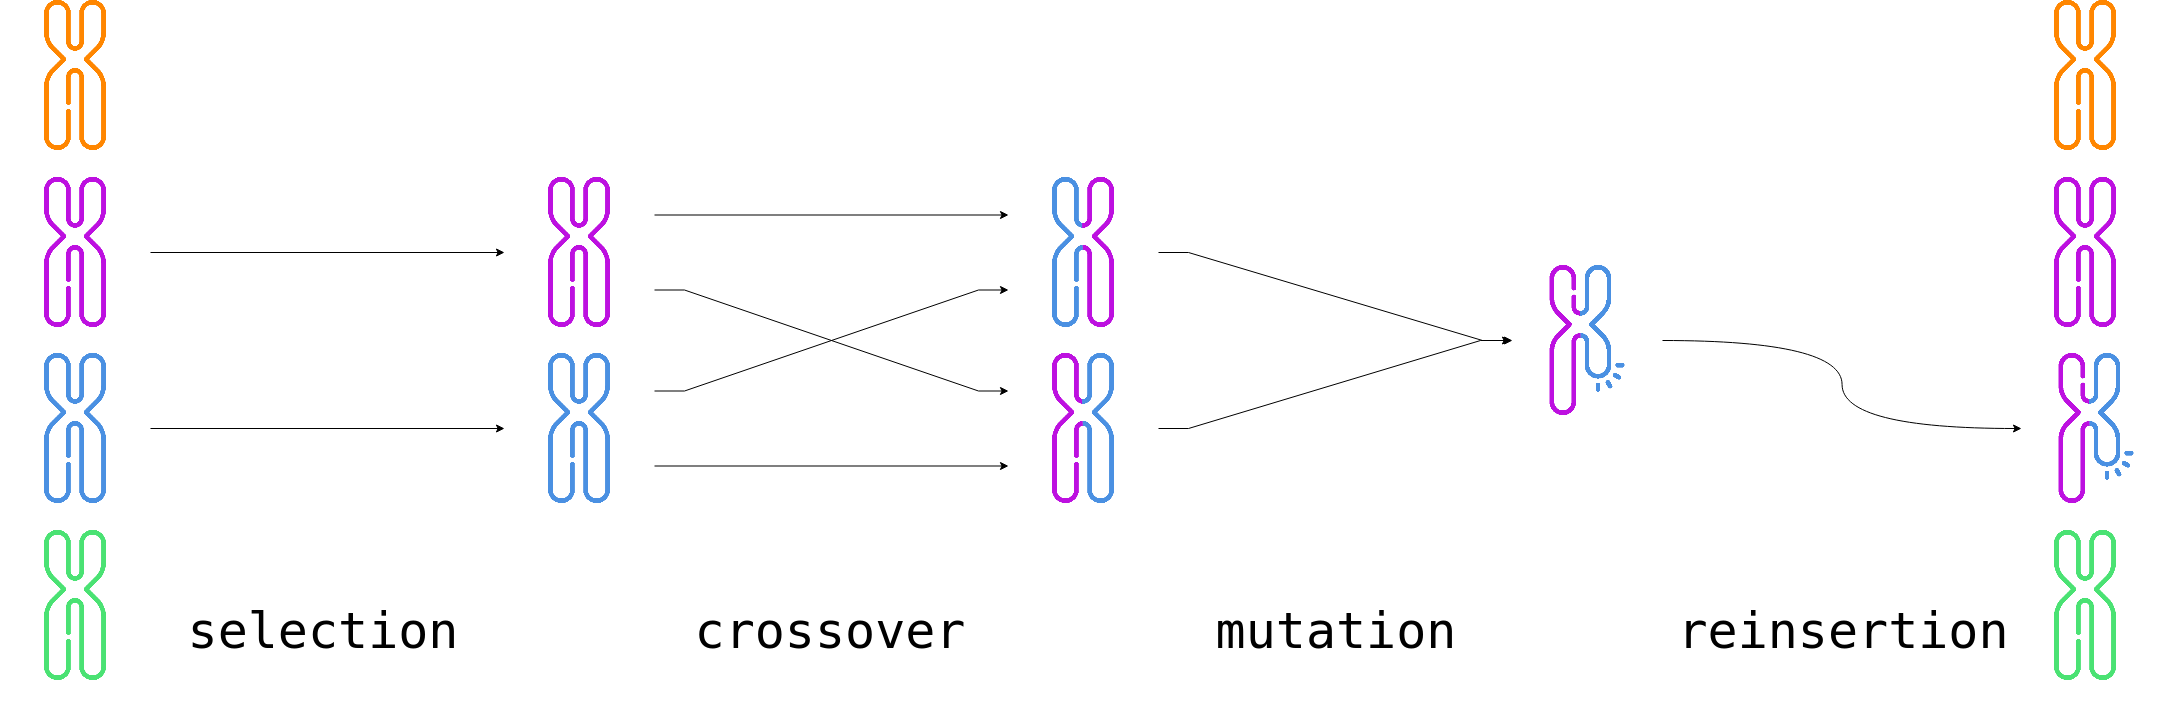
\includegraphics[width=.9\textwidth]{Images/genetic_algo.png}
\end{figure}

\subsection{Genetic Operators}

\paragraph{Tournament Selection}

Tournament selection is a strategy to select individuals for reproduction in which a subset of individuals is selected from the population and the fittest individual is chosen from the subset. Tournament selection is a generic selection operator that can be used in any genetic algorithm.

\paragraph{Mutation}

Mutation is a genetic operator used to introduce new genetic information into the population. In practice, the individual characteristic is modified by applying a random perturbation to its genetic information.

\paragraph{Elitism}

Elitism is a selection strategy in which the fittest individuals are preserved from one generation to the next. It is used to ensure that the fittest individuals are not lost during the evolution process and to speed up the convergence of the algorithm.

\paragraph{Crossover}

Crossover is a genetic operator used to combine the genetic information of two individuals to generate a new individual. In the context of evolutionary algorithms, crossover is used to generate new individuals from the population. The crossover operator is inspired by the natural reproduction process, in which the genetic information of two individuals is combined to generate a new individual. A generic \textit{k-point crossover} operator takes two individuals and a number $k$ as input and returns two new individuals. The two individuals are divided into $k+1$ segments, and the segments are then swapped between the two individuals.

\part{Contributions}\label{part:contributions}
\chapter{Implementing Motors in Rigid Multibody Algorithms}
\label{chp:contrib_ABA}

This chapter describes the formalism and the algorithms involved in the multibody systems forward dynamics reformulation, taking into account motor dynamics in the framework of recursive computation methods. In particular, in the first part, the problem of considering rotor dynamics is addressed by modifying the inertia matrix of the system and introducing a new term in the Coriolis vector. This approach will be referred to as \textit{Inertia-Matrix Method}. While being relatively simple to implement, this method forces some hypotheses that can limit its range of application. An alternative approach is described in the second part of the chapter, in which the process of injecting the motor parameters in the Articulated Body Algorithm (\ac{ABA}) is discussed. In the last section, a comparison between the two approaches is presented, in order to highlight the potentialities and the drawbacks of each method.

\section{Rotor-conditioned Inertia-Matrix Method}

\begin{figure}
    \centering
    \caption{Harmonic Drive Model.}
    \label{fig:harmonic_drive}
    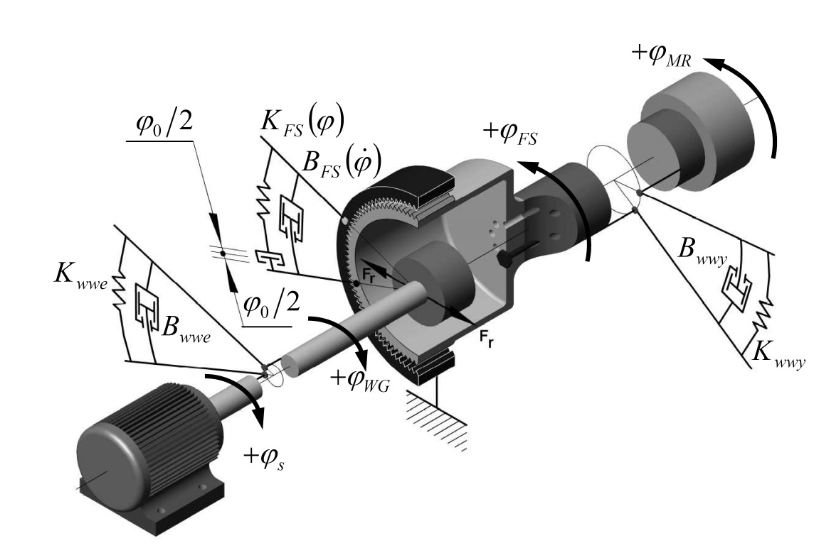
\includegraphics[width=0.8\textwidth]{Images/harmonic_drive.png}
\end{figure}

Starting from the equation of motion of a robot manipulator, as expressed in \cref{sec:back_eom}:

\begin{equation}
    \mathbb{M}(\mathbf{q})\dot{\boldsymbol{\nu}} + \mathbf{h}(\mathbf{q},\boldsymbol{\nu}) = \mathbf{B}\boldsymbol{\tau} + \mathbf{J} ^\top \mathbf{f}
\end{equation}

where $\mathbf{h}(\mathbf{q},\boldsymbol{\nu})$ is the bias forces vector taking into account Coriolis forces and gravity effects, $\mathbf{B}$ is the selector matrix for the joint torques, $\boldsymbol{\tau}$ is actuation torques vector, $\mathbf{J}$ is the Jacobian matrix and $\mathbf{f}$ is the external wrenches vector, we can isolate the terms related to the base link from the rest of the kinematic chain by recalling that:

\begin{align}
    \boldsymbol{\nu} =
    \begin{bmatrix}
        \mathrm{\mathbf{v}} \\
        \dot{\mathbf{s}}
    \end{bmatrix} &  &
    \dot{\boldsymbol{\nu}} =
    \begin{bmatrix}
        \dot{\mathrm{\mathbf{v}}} \\
        \ddot{\mathbf{s}}
    \end{bmatrix}
\end{align}

Therefore, the equation of motion can be rewritten in its matrix form as:

\begin{equation}
    \begin{bmatrix}
        \mathbb{M} _{\mathcal{B}}(\mathbf{q})        & \mathbb{M} _{\mathcal{B}S}(\mathbf{q}) \\
        \mathbb{M} _{\mathcal{B}S} ^\top(\mathbf{q}) & \mathbb{M} _s(\mathbf{q})
    \end{bmatrix}
    \begin{bmatrix}
        \dot{\mathrm{\mathbf{v}}} \\
        \ddot{\mathbf{s}}
    \end{bmatrix}+
    \begin{bmatrix}
        \mathbf{h} _{\mathcal{B}} \\
        \mathbf{h} _S
    \end{bmatrix}=
    \begin{bmatrix}
        \mathbbm{0} \\
        \mathbbm{1}
    \end{bmatrix}
    \boldsymbol{\tau}
    +
    \begin{bmatrix}
        \mathbf{J} _{\mathcal{B}} \\
        \mathbf{J} _S
    \end{bmatrix} ^\top
    \mathbf{f}
\end{equation}

Given that the dynamics of the set of $N _M = n$ motors, each of which is connected to a joint by means of a harmonic drive, graphically represented as in \cref{fig:harmonic_drive} \citep{folga2010}, we can write their equation of motion neglecting the Coulomb friction as:

\begin{equation}
    \mathbb{M} ^M \ddot{\boldsymbol{\theta}} + \mathbf{K}_v \dot{\boldsymbol{\theta}} = \boldsymbol{\tau}_m - \boldsymbol{\tau}
    \label{eqn:mot_dyn}
\end{equation}

where $\mathbf{K}_v \in \mathbb{R}^{n\times n}$ is the diagonal matrix of motor viscous friction coefficients and $\mathbb{M}^M \in \mathbb{R}^{n \times n}$ is the matrix of motors' inertias. Considering that given the set of transmission ratios $\boldsymbol{\Gamma} \in \mathbb{R}^n$, the relation between the joints' velocities and the motors' velocities is:

\begin{align}
    \mathbf{s} = \boldsymbol{\theta} \boldsymbol{\Gamma} &  & \dot{\mathbf{s}} = \frac{d}{dt} \mathbf{s} = \dot{\boldsymbol{\theta}} \boldsymbol{\Gamma} &  & \ddot{\mathbf{s}} = \frac{d^2}{dt^2} \mathbf{s} = \ddot{\boldsymbol{\theta}} \boldsymbol{\Gamma}
\end{align}

Hence, can rewrite the equation \cref{eqn:mot_dyn} in the joints' space as:

\begin{equation}
    \label{eqn:mot_dyn_jointspace}
    \boldsymbol{\tau} = \boldsymbol{\tau}_m - \boldsymbol{\Gamma} ^{-T} (\mathbb{M} ^M\boldsymbol{\Gamma} ^{-1} \ddot{s} + \mathbf{K}_v \boldsymbol{\Gamma} ^{-1}\dot{s})
\end{equation}

Therefore, the \ac{EoM} of the multibody system can be reformulated as:

\begin{equation}
    \underbrace{\begin{bmatrix}
            \mathbb{M} _{\mathcal{B}}(q)        & \mathbb{M} _{\mathcal{B}S}(q)                                                      \\
            \mathbb{M} _{\mathcal{B}S} ^\top(q) & \mathbb{M} _s(q) + \boldsymbol{\Gamma} ^{-T}\mathbb{M} ^M\boldsymbol{\Gamma} ^{-1}
        \end{bmatrix}} _{\bar{\mathbb{M}}(q)}
    \begin{bmatrix}
        \dot{\mathrm{\mathbf{v}}} \\
        \ddot{\mathbf{s}}
    \end{bmatrix}+
    \mathbf{h}
    (q,\boldsymbol{\nu}) =
    \underbrace{\begin{bmatrix}
            \mathbbm{0} \\
            \boldsymbol{\Gamma} ^{-T}
        \end{bmatrix}} _{\mathbf{\bar{B}}}
    \boldsymbol{\tau} _m
    +
    \mathbf{J} ^\top
    \mathbf{f}
    -
    \underbrace{\begin{bmatrix}
            \mathbbm{0} \\
            \boldsymbol{\Gamma} ^{-T}\mathbf{K _v}\boldsymbol{\Gamma} ^{-1}
        \end{bmatrix}} _\mathbf{\bar{K _v}}
    \begin{bmatrix}
        \mathrm{\mathbf{v}} \\
        \dot{\mathbf{s}}
    \end{bmatrix}
\end{equation}

only under the following hypotheses:

\begin{enumerate}
    \item The motors are rigidly attached to the links by the transmission;
    \item The axis of rotation of the motors is aligned with the axis of rotation of the joints;
    \item The gearbox inertia is negligible compared to the link inertia;
    \item The couplings do not introduce any additional friction:
    \item The internal motor friction is modeled as viscous friction only;
    \item The \ac{CoM} of the motor is coincident with its axis of rotation, e.g. the angular momentum of the motor is only due to its spinning motion.
\end{enumerate}

In a more compact form, the \ac{EoM} can be also expressed as:

\begin{equation}
    \mathbf{\bar{M}}(q)\dot{\boldsymbol{\nu}} + \mathbf{h}(q,\boldsymbol{\nu}) = \mathbf{\bar{B}}\boldsymbol{\tau} _m + \mathbf{J} ^\top \mathbf{f} - \bar{\mathbf{K _v}}\boldsymbol{\nu}
\end{equation}

This yields the wanted output from the forward dynamics, the rigid body acceleration vector:

\begin{equation}
    \dot{\boldsymbol{\nu}} = \mathbf{\bar{M}}(q) ^{-1} (\mathbf{\bar{B}}\boldsymbol{\tau} _m + \mathbf{J} ^\top \mathbf{f} - \mathbf{h}(q,\boldsymbol{\nu}) - \bar{\mathbf{K _v}}\boldsymbol{\nu})
\end{equation}

\section{Rotor-conditioned Articulated Body Algorithm}

In \cref{subsec:back_aba} we briefly introduced the recursive relations of the \ac{ABA} algorithm. In this section, we will describe how to modify the algorithm in order to take into account the motor dynamics. The main idea is to consider the rotor as an additional link in the kinematic chain and to modify the inertia matrix and the Coriolis vector accordingly. In particular, we can summarize the hypotheses behind this approach as follows:

\begin{enumerate}
    \item the gearbox inertia is negligible compared to the link inertia;
    \item the motion subspace of the rotor is the same as the motion subspace of the link to which it is attached scaled by the gear ratio, e.g. the free modes of the rotor are the same as the free modes of the link to which it is attached:
    \item The couplings do not introduce any additional friction
    \item The internal motor friction is modeled as viscous friction only;
    \item The \ac{CoM} of the motor is coincident with its axis of rotation, e.g. the angular momentum of the motor is only due to its spinning motion.
\end{enumerate}

With these hypotheses, we can reformulate the motion subspace definition reported in \cref{eqn:subspace} for a rotor attached to joint $i$ as:

\begin{equation}
    \label{eqn:motor_subspace}
    {} ^M \boldsymbol{\Phi} _i = \boldsymbol{\Gamma} _i \boldsymbol{\Phi} _i
\end{equation}


% === FIG: Unconstrained Tree === %
\begin{figure}
    \centering
    \caption{Visual comparison between the unconstrained and constrained kinematic tree.}
    \label{fig:uc_and_constr_tree}
    \subfloat[Constrained System]{
        \resizebox{0.45\textwidth}{!}{
            \tikzset {_djnj2rsc4/.code = {\pgfsetadditionalshadetransform{ \pgftransformshift{\pgfpoint{0 bp } { 0 bp }  }  \pgftransformrotate{-117 }  \pgftransformscale{2 }  }}}
\pgfdeclarehorizontalshading{_idu07h52c}{150bp}{rgb(0bp)=(1,1,1);
    rgb(37.5bp)=(1,1,1);
    rgb(50.08184160505022bp)=(0.95,0.95,0.95);
    rgb(57.64583042689732bp)=(0.88,0.88,0.88);
    rgb(61.33184160505022bp)=(0.96,0.96,0.96);
    rgb(100bp)=(0.96,0.96,0.96)}
\tikzset {_jsyk5ax1n/.code = {\pgfsetadditionalshadetransform{ \pgftransformshift{\pgfpoint{0 bp } { 0 bp }  }  \pgftransformrotate{-117 }  \pgftransformscale{2 }  }}}
\pgfdeclarehorizontalshading{_92edxt770}{150bp}{rgb(0bp)=(1,1,1);
    rgb(37.5bp)=(1,1,1);
    rgb(50.08184160505022bp)=(0.95,0.95,0.95);
    rgb(57.64583042689732bp)=(0.88,0.88,0.88);
    rgb(61.33184160505022bp)=(0.96,0.96,0.96);
    rgb(100bp)=(0.96,0.96,0.96)}
\tikzset {_b0gplq11g/.code = {\pgfsetadditionalshadetransform{ \pgftransformshift{\pgfpoint{0 bp } { 0 bp }  }  \pgftransformrotate{-117 }  \pgftransformscale{2 }  }}}
\pgfdeclarehorizontalshading{_x22po1g8w}{150bp}{rgb(0bp)=(1,1,1);
    rgb(37.5bp)=(1,1,1);
    rgb(50.08184160505022bp)=(0.95,0.95,0.95);
    rgb(57.64583042689732bp)=(0.88,0.88,0.88);
    rgb(61.33184160505022bp)=(0.96,0.96,0.96);
    rgb(100bp)=(0.96,0.96,0.96)}
\tikzset {_ivsfd2s3h/.code = {\pgfsetadditionalshadetransform{ \pgftransformshift{\pgfpoint{0 bp } { 0 bp }  }  \pgftransformrotate{-117 }  \pgftransformscale{2 }  }}}
\pgfdeclarehorizontalshading{_8u84rjokz}{150bp}{rgb(0bp)=(1,1,1);
    rgb(37.5bp)=(1,1,1);
    rgb(50.08184160505022bp)=(0.95,0.95,0.95);
    rgb(57.64583042689732bp)=(0.88,0.88,0.88);
    rgb(61.33184160505022bp)=(0.96,0.96,0.96);
    rgb(100bp)=(0.96,0.96,0.96)}
\tikzset {_5pcd2h8hv/.code = {\pgfsetadditionalshadetransform{ \pgftransformshift{\pgfpoint{0 bp } { 0 bp }  }  \pgftransformrotate{-117 }  \pgftransformscale{2 }  }}}
\pgfdeclarehorizontalshading{_lvec74ltu}{150bp}{rgb(0bp)=(1,1,1);
    rgb(37.5bp)=(1,1,1);
    rgb(50.08184160505022bp)=(0.95,0.95,0.95);
    rgb(57.64583042689732bp)=(0.88,0.88,0.88);
    rgb(61.33184160505022bp)=(0.96,0.96,0.96);
    rgb(100bp)=(0.96,0.96,0.96)}
\tikzset {_37uba45qs/.code = {\pgfsetadditionalshadetransform{ \pgftransformshift{\pgfpoint{0 bp } { 0 bp }  }  \pgftransformrotate{-117 }  \pgftransformscale{2 }  }}}
\pgfdeclarehorizontalshading{_ik4ni4me2}{150bp}{rgb(0bp)=(1,1,1);
    rgb(37.5bp)=(1,1,1);
    rgb(50.08184160505022bp)=(0.95,0.95,0.95);
    rgb(57.64583042689732bp)=(0.88,0.88,0.88);
    rgb(61.33184160505022bp)=(0.96,0.96,0.96);
    rgb(100bp)=(0.96,0.96,0.96)}
\tikzset {_z01vd74d5/.code = {\pgfsetadditionalshadetransform{ \pgftransformshift{\pgfpoint{0 bp } { 0 bp }  }  \pgftransformrotate{-117 }  \pgftransformscale{2 }  }}}
\pgfdeclarehorizontalshading{_rhf2dk4cx}{150bp}{rgb(0bp)=(1,1,1);
    rgb(37.5bp)=(1,1,1);
    rgb(50.08184160505022bp)=(0.95,0.95,0.95);
    rgb(57.64583042689732bp)=(0.88,0.88,0.88);
    rgb(61.33184160505022bp)=(0.96,0.96,0.96);
    rgb(100bp)=(0.96,0.96,0.96)}
\tikzset {_9fj7ssnk1/.code = {\pgfsetadditionalshadetransform{ \pgftransformshift{\pgfpoint{0 bp } { 0 bp }  }  \pgftransformrotate{-117 }  \pgftransformscale{2 }  }}}
\pgfdeclarehorizontalshading{_nn6marsz8}{150bp}{rgb(0bp)=(1,1,1);
    rgb(37.5bp)=(1,1,1);
    rgb(50.08184160505022bp)=(0.95,0.95,0.95);
    rgb(57.64583042689732bp)=(0.88,0.88,0.88);
    rgb(61.33184160505022bp)=(0.96,0.96,0.96);
    rgb(100bp)=(0.96,0.96,0.96)}
\tikzset {_vxd4nfhmk/.code = {\pgfsetadditionalshadetransform{ \pgftransformshift{\pgfpoint{0 bp } { 0 bp }  }  \pgftransformrotate{-117 }  \pgftransformscale{2 }  }}}
\pgfdeclarehorizontalshading{_be3tjpf6d}{150bp}{rgb(0bp)=(1,1,1);
    rgb(37.5bp)=(1,1,1);
    rgb(50.08184160505022bp)=(0.95,0.95,0.95);
    rgb(57.64583042689732bp)=(0.88,0.88,0.88);
    rgb(61.33184160505022bp)=(0.96,0.96,0.96);
    rgb(100bp)=(0.96,0.96,0.96)}
\tikzset {_syya3oz6t/.code = {\pgfsetadditionalshadetransform{ \pgftransformshift{\pgfpoint{0 bp } { 0 bp }  }  \pgftransformrotate{-117 }  \pgftransformscale{2 }  }}}
\pgfdeclarehorizontalshading{_73496xns5}{150bp}{rgb(0bp)=(1,1,1);
    rgb(37.5bp)=(1,1,1);
    rgb(50.08184160505022bp)=(0.95,0.95,0.95);
    rgb(57.64583042689732bp)=(0.88,0.88,0.88);
    rgb(61.33184160505022bp)=(0.96,0.96,0.96);
    rgb(100bp)=(0.96,0.96,0.96)}
\tikzset{every picture/.style={line width=0.75pt}}
\begin{tikzpicture}[x=0.75pt,y=0.75pt,yscale=-1,xscale=1]
    \path  [shading=_idu07h52c,_djnj2rsc4] (360.92,117.33) .. controls (360.92,108.96) and (384.78,102.17) .. (414.21,102.17) .. controls (443.64,102.17) and (467.5,108.96) .. (467.5,117.33) .. controls (467.5,125.71) and (443.64,132.5) .. (414.21,132.5) .. controls (384.78,132.5) and (360.92,125.71) .. (360.92,117.33) -- cycle ;
    \draw  [color={rgb, 255:red, 0; green, 0; blue, 0 }  ,draw opacity=1 ][line width=0.75]  (360.92,117.33) .. controls (360.92,108.96) and (384.78,102.17) .. (414.21,102.17) .. controls (443.64,102.17) and (467.5,108.96) .. (467.5,117.33) .. controls (467.5,125.71) and (443.64,132.5) .. (414.21,132.5) .. controls (384.78,132.5) and (360.92,125.71) .. (360.92,117.33) -- cycle ;
    \path  [shading=_92edxt770,_jsyk5ax1n] (548.22,34.11) .. controls (554.45,39.72) and (543.53,61.99) .. (523.84,83.87) .. controls (504.15,105.75) and (483.14,118.94) .. (476.92,113.33) .. controls (470.69,107.73) and (481.61,85.45) .. (501.3,63.58) .. controls (520.99,41.7) and (542,28.51) .. (548.22,34.11) -- cycle ;
    \draw  [color={rgb, 255:red, 0; green, 0; blue, 0 }  ,draw opacity=1 ][line width=0.75]  (548.22,34.11) .. controls (554.45,39.72) and (543.53,61.99) .. (523.84,83.87) .. controls (504.15,105.75) and (483.14,118.94) .. (476.92,113.33) .. controls (470.69,107.73) and (481.61,85.45) .. (501.3,63.58) .. controls (520.99,41.7) and (542,28.51) .. (548.22,34.11) -- cycle ;
    \path  [shading=_x22po1g8w,_b0gplq11g] (467.5,117.33) .. controls (467.5,114.46) and (469.83,112.13) .. (472.71,112.13) .. controls (475.58,112.13) and (477.92,114.46) .. (477.92,117.33) .. controls (477.92,120.21) and (475.58,122.54) .. (472.71,122.54) .. controls (469.83,122.54) and (467.5,120.21) .. (467.5,117.33) -- cycle ;
    \draw  [color={rgb, 255:red, 0; green, 0; blue, 0 }  ,draw opacity=1 ][line width=0.75]  (467.5,117.33) .. controls (467.5,114.46) and (469.83,112.13) .. (472.71,112.13) .. controls (475.58,112.13) and (477.92,114.46) .. (477.92,117.33) .. controls (477.92,120.21) and (475.58,122.54) .. (472.71,122.54) .. controls (469.83,122.54) and (467.5,120.21) .. (467.5,117.33) -- cycle ;
    \path  [shading=_8u84rjokz,_ivsfd2s3h] (352.22,121.61) .. controls (358.45,127.22) and (347.53,149.49) .. (327.84,171.37) .. controls (308.15,193.25) and (287.14,206.44) .. (280.92,200.83) .. controls (274.69,195.23) and (285.61,172.95) .. (305.3,151.08) .. controls (324.99,129.2) and (346,116.01) .. (352.22,121.61) -- cycle ;
    \draw  [color={rgb, 255:red, 0; green, 0; blue, 0 }  ,draw opacity=1 ][line width=0.75]  (352.22,121.61) .. controls (358.45,127.22) and (347.53,149.49) .. (327.84,171.37) .. controls (308.15,193.25) and (287.14,206.44) .. (280.92,200.83) .. controls (274.69,195.23) and (285.61,172.95) .. (305.3,151.08) .. controls (324.99,129.2) and (346,116.01) .. (352.22,121.61) -- cycle ;
    \path  [shading=_lvec74ltu,_5pcd2h8hv] (350.5,117.33) .. controls (350.5,114.46) and (352.83,112.13) .. (355.71,112.13) .. controls (358.58,112.13) and (360.92,114.46) .. (360.92,117.33) .. controls (360.92,120.21) and (358.58,122.54) .. (355.71,122.54) .. controls (352.83,122.54) and (350.5,120.21) .. (350.5,117.33) -- cycle ;
    \draw  [color={rgb, 255:red, 0; green, 0; blue, 0 }  ,draw opacity=1 ][line width=0.75]  (350.5,117.33) .. controls (350.5,114.46) and (352.83,112.13) .. (355.71,112.13) .. controls (358.58,112.13) and (360.92,114.46) .. (360.92,117.33) .. controls (360.92,120.21) and (358.58,122.54) .. (355.71,122.54) .. controls (352.83,122.54) and (350.5,120.21) .. (350.5,117.33) -- cycle ;
    \path  [shading=_ik4ni4me2,_37uba45qs] (272.46,204.96) .. controls (272.46,202.08) and (274.79,199.75) .. (277.67,199.75) .. controls (280.54,199.75) and (282.87,202.08) .. (282.87,204.96) .. controls (282.87,207.83) and (280.54,210.17) .. (277.67,210.17) .. controls (274.79,210.17) and (272.46,207.83) .. (272.46,204.96) -- cycle ;
    \draw  [color={rgb, 255:red, 0; green, 0; blue, 0 }  ,draw opacity=1 ][line width=0.75]  (272.46,204.96) .. controls (272.46,202.08) and (274.79,199.75) .. (277.67,199.75) .. controls (280.54,199.75) and (282.87,202.08) .. (282.87,204.96) .. controls (282.87,207.83) and (280.54,210.17) .. (277.67,210.17) .. controls (274.79,210.17) and (272.46,207.83) .. (272.46,204.96) -- cycle ;
    \path  [shading=_rhf2dk4cx,_z01vd74d5] (170.95,143.93) .. controls (163.63,148.01) and (146.08,130.48) .. (131.74,104.78) .. controls (117.4,79.08) and (111.7,54.93) .. (119.02,50.85) .. controls (126.33,46.77) and (143.89,64.3) .. (158.23,90) .. controls (172.57,115.7) and (178.26,139.85) .. (170.95,143.93) -- cycle ;
    \draw  [color={rgb, 255:red, 0; green, 0; blue, 0 }  ,draw opacity=1 ][line width=0.75]  (170.95,143.93) .. controls (163.63,148.01) and (146.08,130.48) .. (131.74,104.78) .. controls (117.4,79.08) and (111.7,54.93) .. (119.02,50.85) .. controls (126.33,46.77) and (143.89,64.3) .. (158.23,90) .. controls (172.57,115.7) and (178.26,139.85) .. (170.95,143.93) -- cycle ;
    \path  [shading=_nn6marsz8,_9fj7ssnk1] (179.33,150.95) .. controls (183.31,143.58) and (207.53,148.94) .. (233.43,162.93) .. controls (259.32,176.91) and (277.09,194.22) .. (273.11,201.59) .. controls (269.13,208.96) and (244.91,203.6) .. (219.01,189.62) .. controls (193.12,175.63) and (175.35,158.32) .. (179.33,150.95) -- cycle ;
    \draw  [color={rgb, 255:red, 0; green, 0; blue, 0 }  ,draw opacity=1 ][line width=0.75]  (179.33,150.95) .. controls (183.31,143.58) and (207.53,148.94) .. (233.43,162.93) .. controls (259.32,176.91) and (277.09,194.22) .. (273.11,201.59) .. controls (269.13,208.96) and (244.91,203.6) .. (219.01,189.62) .. controls (193.12,175.63) and (175.35,158.32) .. (179.33,150.95) -- cycle ;
    \path  [shading=_be3tjpf6d,_vxd4nfhmk] (174.79,153.61) .. controls (171.92,153.71) and (169.51,151.45) .. (169.42,148.58) .. controls (169.32,145.7) and (171.58,143.3) .. (174.45,143.2) .. controls (177.33,143.11) and (179.73,145.36) .. (179.83,148.24) .. controls (179.92,151.11) and (177.67,153.52) .. (174.79,153.61) -- cycle ;
    \draw  [color={rgb, 255:red, 0; green, 0; blue, 0 }  ,draw opacity=1 ][line width=0.75]  (174.79,153.61) .. controls (171.92,153.71) and (169.51,151.45) .. (169.42,148.58) .. controls (169.32,145.7) and (171.58,143.3) .. (174.45,143.2) .. controls (177.33,143.11) and (179.73,145.36) .. (179.83,148.24) .. controls (179.92,151.11) and (177.67,153.52) .. (174.79,153.61) -- cycle ;
    \path  [shading=_73496xns5,_syya3oz6t] (540.88,206.7) .. controls (534.23,211.8) and (514.33,196.98) .. (496.44,173.61) .. controls (478.55,150.24) and (469.43,127.17) .. (476.09,122.08) .. controls (482.74,116.98) and (502.63,131.8) .. (520.53,155.17) .. controls (538.42,178.54) and (547.53,201.61) .. (540.88,206.7) -- cycle ;
    \draw  [color={rgb, 255:red, 0; green, 0; blue, 0 }  ,draw opacity=1 ][line width=0.75]  (540.88,206.7) .. controls (534.23,211.8) and (514.33,196.98) .. (496.44,173.61) .. controls (478.55,150.24) and (469.43,127.17) .. (476.09,122.08) .. controls (482.74,116.98) and (502.63,131.8) .. (520.53,155.17) .. controls (538.42,178.54) and (547.53,201.61) .. (540.88,206.7) -- cycle ;
    \draw [color={rgb, 255:red, 74; green, 144; blue, 226 }  ,draw opacity=1 ]   (103.21,151.6) -- (172.62,148.5) ;
    \draw [shift={(174.62,148.41)}, rotate = 177.44] [fill={rgb, 255:red, 74; green, 144; blue, 226 }  ,fill opacity=1 ][line width=0.08]  [draw opacity=0] (12,-3) -- (0,0) -- (12,3) -- cycle    ;
    \draw [color={rgb, 255:red, 74; green, 144; blue, 226 }  ,draw opacity=1 ]   (373.78,57.81) -- (356.29,115.42) ;
    \draw [shift={(355.71,117.33)}, rotate = 286.89] [fill={rgb, 255:red, 74; green, 144; blue, 226 }  ,fill opacity=1 ][line width=0.08]  [draw opacity=0] (12,-3) -- (0,0) -- (12,3) -- cycle    ;
    \draw [color={rgb, 255:red, 74; green, 144; blue, 226 }  ,draw opacity=1 ]   (465.03,205.67) -- (534.45,202.56) ;
    \draw [shift={(536.44,202.47)}, rotate = 177.44] [fill={rgb, 255:red, 74; green, 144; blue, 226 }  ,fill opacity=1 ][line width=0.08]  [draw opacity=0] (12,-3) -- (0,0) -- (12,3) -- cycle    ;
    \draw [color={rgb, 255:red, 74; green, 144; blue, 226 }  ,draw opacity=1 ]   (492.37,61.67) -- (473.37,115.45) ;
    \draw [shift={(472.71,117.33)}, rotate = 289.46] [fill={rgb, 255:red, 74; green, 144; blue, 226 }  ,fill opacity=1 ][line width=0.08]  [draw opacity=0] (12,-3) -- (0,0) -- (12,3) -- cycle    ;
    \draw  [draw opacity=0] (179.21,161.74) .. controls (177.77,162.22) and (176.23,162.48) .. (174.62,162.48) .. controls (166.68,162.48) and (160.25,156.18) .. (160.25,148.41) .. controls (160.25,140.64) and (166.68,134.34) .. (174.62,134.34) .. controls (182.56,134.34) and (189,140.64) .. (189,148.41) .. controls (189,150) and (188.73,151.53) .. (188.23,152.95) -- (174.62,148.41) -- cycle ; \draw [color={rgb, 255:red, 74; green, 144; blue, 226 }  ,draw opacity=1 ]   (179.21,161.74) .. controls (177.77,162.22) and (176.23,162.48) .. (174.62,162.48) .. controls (166.68,162.48) and (160.25,156.18) .. (160.25,148.41) .. controls (160.25,140.64) and (166.68,134.34) .. (174.62,134.34) .. controls (182.56,134.34) and (189,140.64) .. (189,148.41) .. controls (189,149.31) and (188.91,150.18) .. (188.75,151.04) ; \draw [shift={(188.23,152.95)}, rotate = 276.88] [fill={rgb, 255:red, 74; green, 144; blue, 226 }  ,fill opacity=1 ][line width=0.08]  [draw opacity=0] (7.2,-1.8) -- (0,0) -- (7.2,1.8) -- cycle    ;
    \draw  [draw opacity=0] (360.3,130.67) .. controls (358.86,131.15) and (357.31,131.4) .. (355.71,131.4) .. controls (347.77,131.4) and (341.33,125.1) .. (341.33,117.33) .. controls (341.33,109.56) and (347.77,103.26) .. (355.71,103.26) .. controls (363.65,103.26) and (370.08,109.56) .. (370.08,117.33) .. controls (370.08,118.92) and (369.81,120.45) .. (369.32,121.88) -- (355.71,117.33) -- cycle ; \draw [color={rgb, 255:red, 74; green, 144; blue, 226 }  ,draw opacity=1 ]   (360.3,130.67) .. controls (358.86,131.15) and (357.31,131.4) .. (355.71,131.4) .. controls (347.77,131.4) and (341.33,125.1) .. (341.33,117.33) .. controls (341.33,109.56) and (347.77,103.26) .. (355.71,103.26) .. controls (363.65,103.26) and (370.08,109.56) .. (370.08,117.33) .. controls (370.08,118.23) and (370,119.11) .. (369.83,119.96) ; \draw [shift={(369.32,121.88)}, rotate = 276.88] [fill={rgb, 255:red, 74; green, 144; blue, 226 }  ,fill opacity=1 ][line width=0.08]  [draw opacity=0] (7.2,-1.8) -- (0,0) -- (7.2,1.8) -- cycle    ;
    \draw  [draw opacity=0] (477.3,130.67) .. controls (475.86,131.15) and (474.31,131.4) .. (472.71,131.4) .. controls (464.77,131.4) and (458.33,125.1) .. (458.33,117.33) .. controls (458.33,109.56) and (464.77,103.26) .. (472.71,103.26) .. controls (480.65,103.26) and (487.08,109.56) .. (487.08,117.33) .. controls (487.08,118.92) and (486.81,120.45) .. (486.32,121.88) -- (472.71,117.33) -- cycle ; \draw [color={rgb, 255:red, 74; green, 144; blue, 226 }  ,draw opacity=1 ]   (477.3,130.67) .. controls (475.86,131.15) and (474.31,131.4) .. (472.71,131.4) .. controls (464.77,131.4) and (458.33,125.1) .. (458.33,117.33) .. controls (458.33,109.56) and (464.77,103.26) .. (472.71,103.26) .. controls (480.65,103.26) and (487.08,109.56) .. (487.08,117.33) .. controls (487.08,118.23) and (487,119.11) .. (486.83,119.96) ; \draw [shift={(486.32,121.88)}, rotate = 272.62] [fill={rgb, 255:red, 74; green, 144; blue, 226 }  ,fill opacity=1 ][line width=0.08]  [draw opacity=0] (7.2,-1.8) -- (0,0) -- (7.2,1.8) -- cycle    ;
    \draw [color={rgb, 255:red, 74; green, 144; blue, 226 }  ,draw opacity=1 ]   (313.33,253) -- (278.86,206.56) ;
    \draw [shift={(277.67,204.96)}, rotate = 53.41] [fill={rgb, 255:red, 74; green, 144; blue, 226 }  ,fill opacity=1 ][line width=0.08]  [draw opacity=0] (12,-3) -- (0,0) -- (12,3) -- cycle    ;
\end{tikzpicture}

        }
    }
    \subfloat[Uncostrained System]{
        \resizebox{0.45\textwidth}{!}{
            \tikzset {_cuejj3ut6/.code = {\pgfsetadditionalshadetransform{ \pgftransformshift{\pgfpoint{0 bp } { 0 bp }  }  \pgftransformrotate{-117 }  \pgftransformscale{2 }  }}}
\pgfdeclarehorizontalshading{_5ugpqis72}{150bp}{rgb(0bp)=(1,1,1);
    rgb(37.5bp)=(1,1,1);
    rgb(50.08184160505022bp)=(0.95,0.95,0.95);
    rgb(57.64583042689732bp)=(0.88,0.88,0.88);
    rgb(61.33184160505022bp)=(0.96,0.96,0.96);
    rgb(100bp)=(0.96,0.96,0.96)}
\tikzset {_d6bvf3ads/.code = {\pgfsetadditionalshadetransform{ \pgftransformshift{\pgfpoint{0 bp } { 0 bp }  }  \pgftransformrotate{-117 }  \pgftransformscale{2 }  }}}
\pgfdeclarehorizontalshading{_xx64avkmf}{150bp}{rgb(0bp)=(1,1,1);
    rgb(37.5bp)=(1,1,1);
    rgb(50.08184160505022bp)=(0.95,0.95,0.95);
    rgb(57.64583042689732bp)=(0.88,0.88,0.88);
    rgb(61.33184160505022bp)=(0.96,0.96,0.96);
    rgb(100bp)=(0.96,0.96,0.96)}
\tikzset {_gxyzl2ql8/.code = {\pgfsetadditionalshadetransform{ \pgftransformshift{\pgfpoint{0 bp } { 0 bp }  }  \pgftransformrotate{-117 }  \pgftransformscale{2 }  }}}
\pgfdeclarehorizontalshading{_Aokbkkxvx}{150bp}{rgb(0bp)=(1,1,1);
    rgb(37.5bp)=(1,1,1);
    rgb(50.08184160505022bp)=(0.95,0.95,0.95);
    rgb(57.64583042689732bp)=(0.88,0.88,0.88);
    rgb(61.33184160505022bp)=(0.96,0.96,0.96);
    rgb(100bp)=(0.96,0.96,0.96)}
\tikzset {_m8uplal2o/.code = {\pgfsetadditionalshadetransform{ \pgftransformshift{\pgfpoint{0 bp } { 0 bp }  }  \pgftransformrotate{-117 }  \pgftransformscale{2 }  }}}
\pgfdeclarehorizontalshading{_i8uv4t2gq}{150bp}{rgb(0bp)=(1,1,1);
    rgb(37.5bp)=(1,1,1);
    rgb(50.08184160505022bp)=(0.95,0.95,0.95);
    rgb(57.64583042689732bp)=(0.88,0.88,0.88);
    rgb(61.33184160505022bp)=(0.96,0.96,0.96);
    rgb(100bp)=(0.96,0.96,0.96)}
\tikzset {_60x67noot/.code = {\pgfsetadditionalshadetransform{ \pgftransformshift{\pgfpoint{0 bp } { 0 bp }  }  \pgftransformrotate{-117 }  \pgftransformscale{2 }  }}}
\pgfdeclarehorizontalshading{_wjk5bthop}{150bp}{rgb(0bp)=(1,1,1);
    rgb(37.5bp)=(1,1,1);
    rgb(50.08184160505022bp)=(0.95,0.95,0.95);
    rgb(57.64583042689732bp)=(0.88,0.88,0.88);
    rgb(61.33184160505022bp)=(0.96,0.96,0.96);
    rgb(100bp)=(0.96,0.96,0.96)}
\tikzset {_cf91rnvay/.code = {\pgfsetadditionalshadetransform{ \pgftransformshift{\pgfpoint{0 bp } { 0 bp }  }  \pgftransformrotate{-117 }  \pgftransformscale{2 }  }}}
\pgfdeclarehorizontalshading{_e8wxk8n2i}{150bp}{rgb(0bp)=(1,1,1);
    rgb(37.5bp)=(1,1,1);
    rgb(50.08184160505022bp)=(0.95,0.95,0.95);
    rgb(57.64583042689732bp)=(0.88,0.88,0.88);
    rgb(61.33184160505022bp)=(0.96,0.96,0.96);
    rgb(100bp)=(0.96,0.96,0.96)}
\tikzset{every picture/.style={line width=0.75pt}}
\begin{tikzpicture}[x=0.75pt,y=0.75pt,yscale=-1,xscale=1]
    \path  [shading=_5ugpqis72,_cuejj3ut6] (324.59,122.77) .. controls (324.59,114.69) and (345.08,108.14) .. (370.37,108.14) .. controls (395.65,108.14) and (416.14,114.69) .. (416.14,122.77) .. controls (416.14,130.85) and (395.65,137.4) .. (370.37,137.4) .. controls (345.08,137.4) and (324.59,130.85) .. (324.59,122.77) -- cycle ;
    \draw  [color={rgb, 255:red, 0; green, 0; blue, 0 }  ,draw opacity=1 ][line width=0.75]  (324.59,122.77) .. controls (324.59,114.69) and (345.08,108.14) .. (370.37,108.14) .. controls (395.65,108.14) and (416.14,114.69) .. (416.14,122.77) .. controls (416.14,130.85) and (395.65,137.4) .. (370.37,137.4) .. controls (345.08,137.4) and (324.59,130.85) .. (324.59,122.77) -- cycle ;
    \path  [shading=_xx64avkmf,_d6bvf3ads] (485.49,42.5) .. controls (490.83,47.9) and (481.46,69.38) .. (464.54,90.48) .. controls (447.63,111.58) and (429.58,124.31) .. (424.23,118.9) .. controls (418.88,113.5) and (428.26,92.02) .. (445.18,70.92) .. controls (462.09,49.82) and (480.14,37.09) .. (485.49,42.5) -- cycle ;
    \draw  [color={rgb, 255:red, 0; green, 0; blue, 0 }  ,draw opacity=1 ][line width=0.75]  (485.49,42.5) .. controls (490.83,47.9) and (481.46,69.38) .. (464.54,90.48) .. controls (447.63,111.58) and (429.58,124.31) .. (424.23,118.9) .. controls (418.88,113.5) and (428.26,92.02) .. (445.18,70.92) .. controls (462.09,49.82) and (480.14,37.09) .. (485.49,42.5) -- cycle ;
    \path  [shading=_Aokbkkxvx,_gxyzl2ql8] (317.12,126.9) .. controls (322.47,132.3) and (313.09,153.79) .. (296.17,174.89) .. controls (279.26,195.98) and (261.21,208.71) .. (255.86,203.31) .. controls (250.52,197.9) and (259.89,176.42) .. (276.81,155.32) .. controls (293.72,134.22) and (311.77,121.5) .. (317.12,126.9) -- cycle ;
    \draw  [color={rgb, 255:red, 0; green, 0; blue, 0 }  ,draw opacity=1 ][line width=0.75]  (317.12,126.9) .. controls (322.47,132.3) and (313.09,153.79) .. (296.17,174.89) .. controls (279.26,195.98) and (261.21,208.71) .. (255.86,203.31) .. controls (250.52,197.9) and (259.89,176.42) .. (276.81,155.32) .. controls (293.72,134.22) and (311.77,121.5) .. (317.12,126.9) -- cycle ;
    \path  [shading=_i8uv4t2gq,_m8uplal2o] (160.4,145.75) .. controls (154.11,149.69) and (139.04,132.78) .. (126.72,107.99) .. controls (114.4,83.2) and (109.51,59.91) .. (115.79,55.97) .. controls (122.07,52.03) and (137.15,68.94) .. (149.47,93.73) .. controls (161.79,118.53) and (166.68,141.82) .. (160.4,145.75) -- cycle ;
    \draw  [color={rgb, 255:red, 0; green, 0; blue, 0 }  ,draw opacity=1 ][line width=0.75]  (160.4,145.75) .. controls (154.11,149.69) and (139.04,132.78) .. (126.72,107.99) .. controls (114.4,83.2) and (109.51,59.91) .. (115.79,55.97) .. controls (122.07,52.03) and (137.15,68.94) .. (149.47,93.73) .. controls (161.79,118.53) and (166.68,141.82) .. (160.4,145.75) -- cycle ;
    \path  [shading=_wjk5bthop,_60x67noot] (168.6,155.19) .. controls (172.02,148.08) and (192.82,153.25) .. (215.07,166.74) .. controls (237.32,180.23) and (252.58,196.93) .. (249.16,204.04) .. controls (245.74,211.15) and (224.93,205.98) .. (202.69,192.49) .. controls (180.44,179) and (165.18,162.3) .. (168.6,155.19) -- cycle ;
    \draw  [color={rgb, 255:red, 0; green, 0; blue, 0 }  ,draw opacity=1 ][line width=0.75]  (168.6,155.19) .. controls (172.02,148.08) and (192.82,153.25) .. (215.07,166.74) .. controls (237.32,180.23) and (252.58,196.93) .. (249.16,204.04) .. controls (245.74,211.15) and (224.93,205.98) .. (202.69,192.49) .. controls (180.44,179) and (165.18,162.3) .. (168.6,155.19) -- cycle ;
    \path  [shading=_e8wxk8n2i,_cf91rnvay] (479.18,208.97) .. controls (473.47,213.88) and (456.38,199.59) .. (441,177.05) .. controls (425.63,154.51) and (417.81,132.26) .. (423.52,127.34) .. controls (429.23,122.43) and (446.32,136.72) .. (461.69,159.26) .. controls (477.07,181.8) and (484.89,204.06) .. (479.18,208.97) -- cycle ;
    \draw  [color={rgb, 255:red, 0; green, 0; blue, 0 }  ,draw opacity=1 ][line width=0.75]  (479.18,208.97) .. controls (473.47,213.88) and (456.38,199.59) .. (441,177.05) .. controls (425.63,154.51) and (417.81,132.26) .. (423.52,127.34) .. controls (429.23,122.43) and (446.32,136.72) .. (461.69,159.26) .. controls (477.07,181.8) and (484.89,204.06) .. (479.18,208.97) -- cycle ;
    \draw [color={rgb, 255:red, 74; green, 144; blue, 226 }  ,draw opacity=1 ]   (112.21,161.49) -- (171.56,158.51) ;
    \draw [shift={(173.55,158.41)}, rotate = 177.12] [fill={rgb, 255:red, 74; green, 144; blue, 226 }  ,fill opacity=1 ][line width=0.08]  [draw opacity=0] (12,-3) -- (0,0) -- (12,3) -- cycle    ;
    \draw [color={rgb, 255:red, 74; green, 144; blue, 226 }  ,draw opacity=1 ]   (327.97,74.35) -- (312.97,129.84) ;
    \draw [shift={(312.45,131.77)}, rotate = 285.13] [fill={rgb, 255:red, 74; green, 144; blue, 226 }  ,fill opacity=1 ][line width=0.08]  [draw opacity=0] (12,-3) -- (0,0) -- (12,3) -- cycle    ;
    \draw [color={rgb, 255:red, 74; green, 144; blue, 226 }  ,draw opacity=1 ]   (414.02,207.97) -- (473.37,204.99) ;
    \draw [shift={(475.37,204.89)}, rotate = 177.12] [fill={rgb, 255:red, 74; green, 144; blue, 226 }  ,fill opacity=1 ][line width=0.08]  [draw opacity=0] (12,-3) -- (0,0) -- (12,3) -- cycle    ;
    \draw [color={rgb, 255:red, 74; green, 144; blue, 226 }  ,draw opacity=1 ]   (426.51,69.4) -- (410.22,121.19) ;
    \draw [shift={(409.62,123.1)}, rotate = 287.47] [fill={rgb, 255:red, 74; green, 144; blue, 226 }  ,fill opacity=1 ][line width=0.08]  [draw opacity=0] (12,-3) -- (0,0) -- (12,3) -- cycle    ;
    \draw [color={rgb, 255:red, 74; green, 144; blue, 226 }  ,draw opacity=1 ]   (295.44,247.14) -- (260.97,200.71) ;
    \draw [shift={(259.78,199.1)}, rotate = 53.41] [fill={rgb, 255:red, 74; green, 144; blue, 226 }  ,fill opacity=1 ][line width=0.08]  [draw opacity=0] (12,-3) -- (0,0) -- (12,3) -- cycle    ;
\end{tikzpicture}
        }
    }
\end{figure}

An unconstrained system refers to a system where the links are geometrically fixed in place, thereby defining the dynamics of each link independently of the forces interacting with the rest of the system, as represented in \cref{fig:uc_and_constr_tree}. In this setup, similarly to the equation represented in \cref{eqn:motor_subspace}, the rotor experiences the same force of the joint, but the torque is increased proportionally by the gear ratio, as illustrated in \cref{fig:disassembled_motor}

\begin{equation}
    \mathbf{a} ^{uc} _{R _i} = (\mathbb{M} ^M _i) ^{-1}(\boldsymbol{\Phi} _i \frac{\boldsymbol{\tau} _i}{\boldsymbol{\Gamma} _i} - \mathbf{p} ^M _i)
\end{equation}

where $\mathbb{M} ^M _i$ is the rotor inertia matrix, $\mathbf{p} ^M _i$ is the bias force of the rotor defined recalling \cref{eqn:biasforce} as  $\mathbf{p} ^M _i = {} ^M \mathbf{v} _i\times ^* \mathbb{M} ^M _i {} ^M \mathbf{v} _i$, where ${} ^M \mathbf{v} = \mathbf{v} _{\lambda (i)} + {} ^M \boldsymbol{\Phi} _i \dot{\mathbf{s}} _i$ and $\boldsymbol{\Gamma} _i$ is the gear ratio.

Beginning with the Gaussian principle of least constraint, the objective is to determine the joint accelerations $\ddot{\mathbf{s}}$ that fulfill the equation of motion as described in \cref{eqn:equation_of_motion}. This task can be framed as a constrained optimization problem:

\begin{align}
    \label{eqn:aba_optim}
    \begin{aligned}
         & \underset{\ddot{\mathbf{s}}}{\text{minimize}}
         &                                               & \sum _{i \in \mathbb{L}} (\mathbf{a}_i - \mathbf{a} _i ^{\text{uc} }) ^\top \mathbb{I} _i(\mathbf{a}_i - \mathbf{a} ^{\text{uc}} _i) \\
         & \text{subject to}
         &                                               & \{\mathbf{a}_i\} \text{ satisfying geometric constraints}
    \end{aligned}
\end{align}

where $\mathbf{a} _i$ and $\mathbf{a} _i ^{\text{uc}}$ are respectively the costrained and the unconstrained acceleration of the $i$-th body, and $\mathbb{I} _i$ is its spatial inertia.


% === FIG: Unconstrained Motor === %
\begin{figure}
    \centering
    \caption{Uncostrained Motor Model on Kinematic Chain.}
    \label{fig:disassembled_motor}
    \resizebox{0.8\textwidth}{!}{
        \tikzset {_05o9hrnmr/.code = {\pgfsetadditionalshadetransform{ \pgftransformshift{\pgfpoint{0 bp } { 0 bp }  }  \pgftransformrotate{-117 }  \pgftransformscale{2 }  }}}
\pgfdeclarehorizontalshading{_3050tuc2o}{150bp}{rgb(0bp)=(1,1,1);
    rgb(37.5bp)=(1,1,1);
    rgb(50.08184160505022bp)=(0.95,0.95,0.95);
    rgb(57.64583042689732bp)=(0.88,0.88,0.88);
    rgb(61.33184160505022bp)=(0.96,0.96,0.96);
    rgb(100bp)=(0.96,0.96,0.96)}
\tikzset {_sukiq91mf/.code = {\pgfsetadditionalshadetransform{ \pgftransformshift{\pgfpoint{0 bp } { 0 bp }  }  \pgftransformrotate{-117 }  \pgftransformscale{2 }  }}}
\pgfdeclarehorizontalshading{_0sr9vccbw}{150bp}{rgb(0bp)=(1,1,1);
    rgb(37.5bp)=(1,1,1);
    rgb(50.08184160505022bp)=(0.95,0.95,0.95);
    rgb(57.64583042689732bp)=(0.88,0.88,0.88);
    rgb(61.33184160505022bp)=(0.96,0.96,0.96);
    rgb(100bp)=(0.96,0.96,0.96)}
\tikzset {_g1y39j6wc/.code = {\pgfsetadditionalshadetransform{ \pgftransformshift{\pgfpoint{0 bp } { 0 bp }  }  \pgftransformrotate{-117 }  \pgftransformscale{2 }  }}}
\pgfdeclarehorizontalshading{_7o0aby0ry}{150bp}{rgb(0bp)=(1,1,1);
    rgb(37.5bp)=(1,1,1);
    rgb(50.08184160505022bp)=(0.95,0.95,0.95);
    rgb(57.64583042689732bp)=(0.88,0.88,0.88);
    rgb(61.33184160505022bp)=(0.96,0.96,0.96);
    rgb(100bp)=(0.96,0.96,0.96)}
\tikzset {_sx585m017/.code = {\pgfsetadditionalshadetransform{ \pgftransformshift{\pgfpoint{0 bp } { 0 bp }  }  \pgftransformrotate{-117 }  \pgftransformscale{2 }  }}}
\pgfdeclarehorizontalshading{_vrosuyu06}{150bp}{rgb(0bp)=(1,1,1);
    rgb(37.5bp)=(1,1,1);
    rgb(50.08184160505022bp)=(0.95,0.95,0.95);
    rgb(57.64583042689732bp)=(0.88,0.88,0.88);
    rgb(61.33184160505022bp)=(0.96,0.96,0.96);
    rgb(100bp)=(0.96,0.96,0.96)}
\tikzset {_xv91ptrsn/.code = {\pgfsetadditionalshadetransform{ \pgftransformshift{\pgfpoint{0 bp } { 0 bp }  }  \pgftransformrotate{-76 }  \pgftransformscale{2 }  }}}
\pgfdeclarehorizontalshading{_nhul4iann}{150bp}{rgb(0bp)=(0.65,0.81,0.87);
    rgb(37.5bp)=(0.65,0.81,0.87);
    rgb(50.16369138445173bp)=(0.29,0.56,0.89);
    rgb(62.5bp)=(0.29,0.56,0.89);
    rgb(100bp)=(0.29,0.56,0.89)}
\tikzset{_bbvmxj1ed/.code = {\pgfsetadditionalshadetransform{\pgftransformshift{\pgfpoint{0 bp } { 0 bp }  }  \pgftransformrotate{-76 }  \pgftransformscale{2 } }}}
\pgfdeclarehorizontalshading{_8bw6u8f13} {150bp} {color(0bp)=(transparent!0);
    color(37.5bp)=(transparent!0);
    color(50.16369138445173bp)=(transparent!84);
    color(62.5bp)=(transparent!35);
    color(100bp)=(transparent!35) }
\pgfdeclarefading{_wvboa5dv4}{\tikz \fill[shading=_8bw6u8f13,_bbvmxj1ed] (0,0) rectangle (50bp,50bp); }
\tikzset {_8d2g8fv7x/.code = {\pgfsetadditionalshadetransform{ \pgftransformshift{\pgfpoint{0 bp } { 0 bp }  }  \pgftransformrotate{-117 }  \pgftransformscale{2 }  }}}
\pgfdeclarehorizontalshading{_jpssjqb7l}{150bp}{rgb(0bp)=(1,1,1);
    rgb(37.5bp)=(1,1,1);
    rgb(50.08184160505022bp)=(0.95,0.95,0.95);
    rgb(57.64583042689732bp)=(0.88,0.88,0.88);
    rgb(61.33184160505022bp)=(0.96,0.96,0.96);
    rgb(100bp)=(0.96,0.96,0.96)}
\tikzset {_u5ghg7uoq/.code = {\pgfsetadditionalshadetransform{ \pgftransformshift{\pgfpoint{0 bp } { 0 bp }  }  \pgftransformrotate{-117 }  \pgftransformscale{2 }  }}}
\pgfdeclarehorizontalshading{_12u7vly4x}{150bp}{rgb(0bp)=(1,1,1);
    rgb(37.5bp)=(1,1,1);
    rgb(50.08184160505022bp)=(0.95,0.95,0.95);
    rgb(57.64583042689732bp)=(0.88,0.88,0.88);
    rgb(61.33184160505022bp)=(0.96,0.96,0.96);
    rgb(100bp)=(0.96,0.96,0.96)}
\tikzset {_v3dyi8y7c/.code = {\pgfsetadditionalshadetransform{ \pgftransformshift{\pgfpoint{0 bp } { 0 bp }  }  \pgftransformrotate{-117 }  \pgftransformscale{2 }  }}}
\pgfdeclarehorizontalshading{_ww5cykcyv}{150bp}{rgb(0bp)=(1,1,1);
    rgb(37.5bp)=(1,1,1);
    rgb(50.08184160505022bp)=(0.95,0.95,0.95);
    rgb(57.64583042689732bp)=(0.88,0.88,0.88);
    rgb(61.33184160505022bp)=(0.96,0.96,0.96);
    rgb(100bp)=(0.96,0.96,0.96)}
\tikzset {_xcgjq768j/.code = {\pgfsetadditionalshadetransform{ \pgftransformshift{\pgfpoint{0 bp } { 0 bp }  }  \pgftransformrotate{-76 }  \pgftransformscale{2 }  }}}
\pgfdeclarehorizontalshading{_ca8b4kvm3}{150bp}{rgb(0bp)=(0.65,0.81,0.87);
    rgb(37.5bp)=(0.65,0.81,0.87);
    rgb(50.16369138445173bp)=(0.29,0.56,0.89);
    rgb(62.5bp)=(0.29,0.56,0.89);
    rgb(100bp)=(0.29,0.56,0.89)}
\tikzset{_uzy9jcyew/.code = {\pgfsetadditionalshadetransform{\pgftransformshift{\pgfpoint{0 bp } { 0 bp }  }  \pgftransformrotate{-76 }  \pgftransformscale{2 } }}}
\pgfdeclarehorizontalshading{_gao6d2oe3} {150bp} {color(0bp)=(transparent!0);
    color(37.5bp)=(transparent!0);
    color(50.16369138445173bp)=(transparent!84);
    color(62.5bp)=(transparent!35);
    color(100bp)=(transparent!35) }
\pgfdeclarefading{_iy7jvpss4}{\tikz \fill[shading=_gao6d2oe3,_uzy9jcyew] (0,0) rectangle (50bp,50bp); }
\tikzset{every picture/.style={line width=0.75pt}}
\begin{tikzpicture}[x=0.75pt,y=0.75pt,yscale=-1,xscale=1]
    \path  [shading=_3050tuc2o,_05o9hrnmr] (217.98,165.87) .. controls (217.98,157.49) and (241.84,150.7) .. (271.27,150.7) .. controls (300.71,150.7) and (324.57,157.49) .. (324.57,165.87) .. controls (324.57,174.24) and (300.71,181.03) .. (271.27,181.03) .. controls (241.84,181.03) and (217.98,174.24) .. (217.98,165.87) -- cycle ;
    \draw  [color={rgb, 255:red, 0; green, 0; blue, 0 }  ,draw opacity=1 ][line width=0.75]  (217.98,165.87) .. controls (217.98,157.49) and (241.84,150.7) .. (271.27,150.7) .. controls (300.71,150.7) and (324.57,157.49) .. (324.57,165.87) .. controls (324.57,174.24) and (300.71,181.03) .. (271.27,181.03) .. controls (241.84,181.03) and (217.98,174.24) .. (217.98,165.87) -- cycle ;
    \path  [shading=_0sr9vccbw,_sukiq91mf] (405.29,82.65) .. controls (411.51,88.25) and (400.6,110.53) .. (380.91,132.4) .. controls (361.22,154.28) and (340.21,167.47) .. (333.98,161.87) .. controls (327.76,156.26) and (338.67,133.99) .. (358.36,112.11) .. controls (378.05,90.23) and (399.06,77.04) .. (405.29,82.65) -- cycle ;
    \draw  [color={rgb, 255:red, 0; green, 0; blue, 0 }  ,draw opacity=1 ][line width=0.75]  (405.29,82.65) .. controls (411.51,88.25) and (400.6,110.53) .. (380.91,132.4) .. controls (361.22,154.28) and (340.21,167.47) .. (333.98,161.87) .. controls (327.76,156.26) and (338.67,133.99) .. (358.36,112.11) .. controls (378.05,90.23) and (399.06,77.04) .. (405.29,82.65) -- cycle ;
    \path  [shading=_7o0aby0ry,_g1y39j6wc] (324.57,165.87) .. controls (324.57,162.99) and (326.9,160.66) .. (329.77,160.66) .. controls (332.65,160.66) and (334.98,162.99) .. (334.98,165.87) .. controls (334.98,168.74) and (332.65,171.07) .. (329.77,171.07) .. controls (326.9,171.07) and (324.57,168.74) .. (324.57,165.87) -- cycle ;
    \draw  [color={rgb, 255:red, 0; green, 0; blue, 0 }  ,draw opacity=1 ][line width=0.75]  (324.57,165.87) .. controls (324.57,162.99) and (326.9,160.66) .. (329.77,160.66) .. controls (332.65,160.66) and (334.98,162.99) .. (334.98,165.87) .. controls (334.98,168.74) and (332.65,171.07) .. (329.77,171.07) .. controls (326.9,171.07) and (324.57,168.74) .. (324.57,165.87) -- cycle ;
    \path  [shading=_vrosuyu06,_sx585m017] (142.89,184.95) .. controls (149.11,190.55) and (138.2,212.83) .. (118.51,234.7) .. controls (98.82,256.58) and (77.81,269.77) .. (71.58,264.17) .. controls (65.36,258.56) and (76.27,236.29) .. (95.96,214.41) .. controls (115.65,192.53) and (136.66,179.34) .. (142.89,184.95) -- cycle ;
    \draw  [color={rgb, 255:red, 0; green, 0; blue, 0 }  ,draw opacity=1 ][line width=0.75]  (142.89,184.95) .. controls (149.11,190.55) and (138.2,212.83) .. (118.51,234.7) .. controls (98.82,256.58) and (77.81,269.77) .. (71.58,264.17) .. controls (65.36,258.56) and (76.27,236.29) .. (95.96,214.41) .. controls (115.65,192.53) and (136.66,179.34) .. (142.89,184.95) -- cycle ;
    \path  [shading=_nhul4iann,_xv91ptrsn,path fading= _wvboa5dv4 ,fading transform={xshift=2}] (145.57,179.47) .. controls (145.57,176.59) and (147.9,174.26) .. (150.77,174.26) .. controls (153.65,174.26) and (155.98,176.59) .. (155.98,179.47) .. controls (155.98,182.34) and (153.65,184.67) .. (150.77,184.67) .. controls (147.9,184.67) and (145.57,182.34) .. (145.57,179.47) -- cycle ;
    \draw  [color={rgb, 255:red, 74; green, 144; blue, 226 }  ,draw opacity=1 ][line width=0.75]  (145.57,179.47) .. controls (145.57,176.59) and (147.9,174.26) .. (150.77,174.26) .. controls (153.65,174.26) and (155.98,176.59) .. (155.98,179.47) .. controls (155.98,182.34) and (153.65,184.67) .. (150.77,184.67) .. controls (147.9,184.67) and (145.57,182.34) .. (145.57,179.47) -- cycle ;
    \path  [shading=_jpssjqb7l,_8d2g8fv7x] (63.12,268.29) .. controls (63.12,265.42) and (65.46,263.08) .. (68.33,263.08) .. controls (71.21,263.08) and (73.54,265.42) .. (73.54,268.29) .. controls (73.54,271.17) and (71.21,273.5) .. (68.33,273.5) .. controls (65.46,273.5) and (63.12,271.17) .. (63.12,268.29) -- cycle ;
    \draw  [color={rgb, 255:red, 0; green, 0; blue, 0 }  ,draw opacity=1 ][line width=0.75]  (63.12,268.29) .. controls (63.12,265.42) and (65.46,263.08) .. (68.33,263.08) .. controls (71.21,263.08) and (73.54,265.42) .. (73.54,268.29) .. controls (73.54,271.17) and (71.21,273.5) .. (68.33,273.5) .. controls (65.46,273.5) and (63.12,271.17) .. (63.12,268.29) -- cycle ;
    \path  [shading=_12u7vly4x,_u5ghg7uoq] (397.95,255.24) .. controls (391.3,260.33) and (371.4,245.51) .. (353.51,222.14) .. controls (335.61,198.77) and (326.5,175.7) .. (333.15,170.61) .. controls (339.8,165.52) and (359.7,180.33) .. (377.59,203.7) .. controls (395.48,227.07) and (404.6,250.14) .. (397.95,255.24) -- cycle ;
    \draw  [color={rgb, 255:red, 0; green, 0; blue, 0 }  ,draw opacity=1 ][line width=0.75]  (397.95,255.24) .. controls (391.3,260.33) and (371.4,245.51) .. (353.51,222.14) .. controls (335.61,198.77) and (326.5,175.7) .. (333.15,170.61) .. controls (339.8,165.52) and (359.7,180.33) .. (377.59,203.7) .. controls (395.48,227.07) and (404.6,250.14) .. (397.95,255.24) -- cycle ;
    \path  [shading=_ww5cykcyv,_v3dyi8y7c] (36.54,315.83) .. controls (34.76,312.23) and (33.77,308.26) .. (33.77,304.1) .. controls (33.77,287.53) and (49.44,274.1) .. (68.77,274.1) .. controls (88.1,274.1) and (103.77,287.53) .. (103.77,304.1) .. controls (103.77,308.26) and (102.78,312.23) .. (100.99,315.83) -- cycle ;
    \draw   (36.54,315.83) .. controls (34.76,312.23) and (33.77,308.26) .. (33.77,304.1) .. controls (33.77,287.53) and (49.44,274.1) .. (68.77,274.1) .. controls (88.1,274.1) and (103.77,287.53) .. (103.77,304.1) .. controls (103.77,308.26) and (102.78,312.23) .. (100.99,315.83) -- cycle ;
    \draw [color={rgb, 255:red, 0; green, 0; blue, 0 }  ,draw opacity=0.5 ]   (37.04,315.83) -- (44.63,323.66) ;
    \draw [color={rgb, 255:red, 0; green, 0; blue, 0 }  ,draw opacity=0.5 ]   (99.49,315.83) -- (107.07,323.66) ;
    \draw [color={rgb, 255:red, 0; green, 0; blue, 0 }  ,draw opacity=0.5 ]   (42.29,315.83) -- (49.88,323.66) ;
    \draw [color={rgb, 255:red, 0; green, 0; blue, 0 }  ,draw opacity=0.5 ]   (47.29,315.58) -- (54.88,323.41) ;
    \draw [color={rgb, 255:red, 0; green, 0; blue, 0 }  ,draw opacity=0.5 ]   (52.54,315.58) -- (60.13,323.41) ;
    \draw [color={rgb, 255:red, 0; green, 0; blue, 0 }  ,draw opacity=0.5 ]   (57.54,315.58) -- (65.13,323.41) ;
    \draw [color={rgb, 255:red, 0; green, 0; blue, 0 }  ,draw opacity=0.5 ]   (62.79,315.58) -- (70.38,323.41) ;
    \draw [color={rgb, 255:red, 0; green, 0; blue, 0 }  ,draw opacity=0.5 ]   (67.79,315.58) -- (75.38,323.41) ;
    \draw [color={rgb, 255:red, 0; green, 0; blue, 0 }  ,draw opacity=0.5 ]   (73.04,315.58) -- (80.63,323.41) ;
    \draw [color={rgb, 255:red, 0; green, 0; blue, 0 }  ,draw opacity=0.5 ]   (78.54,315.58) -- (86.13,323.41) ;
    \draw [color={rgb, 255:red, 0; green, 0; blue, 0 }  ,draw opacity=0.5 ]   (83.79,315.58) -- (91.38,323.41) ;
    \draw [color={rgb, 255:red, 0; green, 0; blue, 0 }  ,draw opacity=0.5 ]   (89.04,315.58) -- (96.63,323.41) ;
    \draw [color={rgb, 255:red, 0; green, 0; blue, 0 }  ,draw opacity=0.5 ]   (94.29,315.58) -- (101.88,323.41) ;
    \path  [shading=_ca8b4kvm3,_xcgjq768j,path fading= _iy7jvpss4 ,fading transform={xshift=2}] (166.2,161.07) -- (205.22,155.6) -- (208.56,179.42) -- (169.54,184.89) -- cycle ;
    \draw  [color={rgb, 255:red, 74; green, 144; blue, 226 }  ,draw opacity=1 ] (166.2,161.07) -- (205.22,155.6) -- (208.56,179.42) -- (169.54,184.89) -- cycle ;
    \draw  [draw opacity=0] (143.43,170.08) .. controls (145.47,168.57) and (148.01,167.67) .. (150.77,167.67) .. controls (157.48,167.67) and (162.91,172.95) .. (162.91,179.47) .. controls (162.91,182.49) and (161.74,185.25) .. (159.82,187.34) -- (150.77,179.47) -- cycle ; \draw [color={rgb, 255:red, 74; green, 144; blue, 226 }  ,draw opacity=1 ]   (143.43,170.08) .. controls (145.47,168.57) and (148.01,167.67) .. (150.77,167.67) .. controls (157.48,167.67) and (162.91,172.95) .. (162.91,179.47) .. controls (162.91,181.8) and (162.22,183.97) .. (161.02,185.79) ; \draw [shift={(159.82,187.34)}, rotate = 298.66] [fill={rgb, 255:red, 74; green, 144; blue, 226 }  ,fill opacity=1 ][line width=0.08]  [draw opacity=0] (7.2,-1.8) -- (0,0) -- (7.2,1.8) -- cycle    ;
    \draw  [draw opacity=0] (224.27,177.29) .. controls (223.16,177.3) and (222.03,177.16) .. (220.9,176.85) .. controls (214.43,175.11) and (210.56,168.6) .. (212.25,162.31) .. controls (213.47,157.81) and (217.2,154.64) .. (221.59,153.84) -- (223.97,165.47) -- cycle ; \draw [color={rgb, 255:red, 74; green, 144; blue, 226 }  ,draw opacity=1 ]   (222.27,177.14) .. controls (221.82,177.07) and (221.36,176.98) .. (220.9,176.85) .. controls (214.43,175.11) and (210.56,168.6) .. (212.25,162.31) .. controls (213.47,157.81) and (217.2,154.64) .. (221.59,153.84) ;  \draw [shift={(224.27,177.29)}, rotate = 193.28] [fill={rgb, 255:red, 74; green, 144; blue, 226 }  ,fill opacity=1 ][line width=0.08]  [draw opacity=0] (7.2,-1.8) -- (0,0) -- (7.2,1.8) -- cycle    ;
    \draw (214.4,132.4) node [anchor=north west][inner sep=0.75pt]    {$\textcolor[rgb]{0.29,0.56,0.89}{\boldsymbol{\tau }}\textcolor[rgb]{0.29,0.56,0.89}{_{i}}$};
    \draw (122.8,129.2) node [anchor=north west][inner sep=0.75pt]    {$\textcolor[rgb]{0.29,0.56,0.89}{\frac{\boldsymbol{\tau }_{i}}{\boldsymbol{\Gamma }_{i}}}$};
    \draw (93.6,213.6) node [anchor=north west][inner sep=0.75pt]    {$\textcolor[rgb]{0.29,0.56,0.89}{\lambda }\textcolor[rgb]{0.29,0.56,0.89}{(}\textcolor[rgb]{0.29,0.56,0.89}{i}\textcolor[rgb]{0.29,0.56,0.89}{)}$};
    \draw (266,157.4) node [anchor=north west][inner sep=0.75pt]    {$\textcolor[rgb]{0.29,0.56,0.89}{i}$};
\end{tikzpicture}
    }
\end{figure}

In the constrained case instead, the admissible accelerations of each link are limited by the acceleration of the rest of the kinematic chain.

\begin{equation}
    \mathbf{a} _i = \boldsymbol{\Phi} _i \ddot{\mathbf{s}} _i + \underbrace{\mathbf{v} _i \times ^* \boldsymbol{\Phi} _i \dot{\mathbf{s}}} _{\mathbf{c} _i}
\end{equation}

where $\mathbf{c} _i$ is the Coriolis acceleration. The equation for the rotor is then obtained similarly:

\begin{equation}
    {} ^M \mathbf{a} _i = {} ^M \boldsymbol{\Phi} _i \ddot{\mathbf{s}} _i + \underbrace{{} ^M \mathbf{v} _i \times ^* {} ^M\boldsymbol{\Phi} _i \dot{\mathbf{s}}} _{{} ^M \mathbf{c} _i}
\end{equation}

This yields the modified version of the constrained problem of \cref{eqn:aba_optim}:

\begin{align}
    \underset{\ddot{\mathbf{s}}}{\arg \min} & \qquad (\mathbf{a} _i - \mathbf{a} _i ^{uc}) \mathbb{I} ^A _i (\mathbf{a} _i - \mathbf{a} _i ^{uc}) + ({} ^M \mathbf{a} _i - {} ^M \mathbf{a} _i ^{uc}) \mathbb{M} ^M _i ({} ^M \mathbf{a} _i - {} ^M \mathbf{a} _i ^{uc}) \nonumber                         \\
    \text{where }                           & \qquad \mathbf{a} _i = \mathbf{a} _{\lambda (i)} + \boldsymbol{\Phi} _i \ddot{\mathbf{s}} _i + \mathbf{c} _i \text{ and } {} ^M \mathbf{a} _i = \mathbf{a} _{\lambda (i)} + {} ^M  \boldsymbol{\Phi} _i \ddot{\mathbf{s}} _i + {} ^M \mathbf{c} _i \nonumber \\
\end{align}

\begin{equation}
    \begin{aligned}
         & \underset{\ddot{\mathbf{s}}}{\arg \min} &  & (\mathbf{a} _i - \mathbf{a} _i ^{uc}) \mathbb{I} ^A _i (\mathbf{a} _i - \mathbf{a} _i ^{uc}) + ({} ^M \mathbf{a} _i - {} ^M \mathbf{a} _i ^{uc}) \mathbb{M} ^M _i ({} ^M \mathbf{a} _i - {} ^M \mathbf{a} _i ^{uc})                                   \\
         & \text{where }                           &  & \mathbf{a} _i = \mathbf{a} _{\lambda (i)} + \boldsymbol{\Phi} _i \ddot{\mathbf{s}} _i + \mathbf{c} _i \text{ and } {} ^M \mathbf{a} _i = \mathbf{a} _{\lambda (i)} + {} ^M  \boldsymbol{\Phi} _i \ddot{\mathbf{s}} _i + {} ^M \mathbf{c} _i \nonumber
    \end{aligned}
\end{equation}

whose objective function can be then expanded as:

\begin{flalign}
    J = & \ \mathbf{a} ^\top _i \mathbb{I} ^A _i \mathbf{a} _i - 2\mathbf{a} ^\top _i \mathbb{I} ^A _i \mathbf{a} ^{uc} _i + (\mathbf{a} ^{uc} _i) ^\top \mathbb{I} ^A _i \mathbf{a} ^{uc} _i +                             \\
        & + {} ^M \mathbf{a} ^\top _i \mathbb{M} ^M _i {} ^M \mathbf{a} _i - 2\mathbf{a} ^\top _i \mathbb{M} ^M _i {} ^M \mathbf{a} ^{uc} _i + ({} ^M \mathbf{a} ^{uc} _i) ^\top \mathbb{M} ^M _i {} ^M \mathbf{a} ^{uc} _i
\end{flalign}

as any term that is not quadratic in $\ddot{\mathbf{s}}$ is zero when computing the gradient, we can extract the two relevant terms of $J$:

\begin{equation}
    \begin{aligned}
        J _1 & = \mathbf{a} ^\top _i \mathbb{I} ^A _i \mathbf{a} _i - 2\mathbf{a} ^\top _i \mathbb{I} ^A _i \mathbf{a} ^{uc} _i                          \\
        J _2 & = {} ^M \mathbf{a} ^\top _i \mathbb{M} ^M _i {} ^M \mathbf{a} _i - 2 {} ^M \mathbf{a} ^\top _i \mathbb{M} ^M _i {} ^M \mathbf{a} ^{uc} _i
    \end{aligned}
\end{equation}

substituting the constraints in the objective function, removing terms not depending on $\ddot{\mathbf{s}}$ and taking the gradient, the following equation is obtained:

\begin{align}
    \frac{\partial J _1}{\partial \ddot{\mathbf{s}} _i} & = 2 \boldsymbol{\Phi} ^\top _i \mathbb{I} ^A _i \boldsymbol{\Phi} _i \ddot{\mathbf{s}} _i + 2 \boldsymbol{\Phi} ^\top _i \mathbb{I} ^A _i (\mathbf{a} _{\lambda (i)} + \mathbf{c} _i) - 2 \boldsymbol{\Phi} ^\top _i \mathbb{I} ^A _i \mathbf{a} ^{uc} _i \nonumber                                        \\
    \frac{\partial J _2}{\partial \ddot{\mathbf{s}} _i} & = 2 {} ^M \boldsymbol{\Phi} ^\top _i \mathbb{M} ^M _i {} ^M \boldsymbol{\Phi} _i \ddot{\mathbf{s}} _i + 2 {} ^M  \boldsymbol{\Phi} ^\top _i \mathbb{M} ^M _i (\mathbf{a} _{\lambda (i)} + {} ^M  \mathbf{c} _i) - 2 {} ^M \boldsymbol{\Phi} ^\top _i \mathbb{M} ^M _i {} ^M \mathbf{a} ^{uc} _i  \nonumber
\end{align}

Adding up the two terms and defining for compactness:

\begin{equation}
    \mathbf{D} _i = \boldsymbol{\Phi} ^\top _i \mathbb{I} ^A _i \boldsymbol{\Phi} _i + {} ^M \boldsymbol{\Phi} ^\top _i \mathbb{M} ^M _i {} ^M \boldsymbol{\Phi} _i
\end{equation}

we get to:

\begin{equation}
    \label{eqn:aba_jointacc}
    \ddot{\mathbf{s}} _i = \mathbf{D} _i ^{-1} (\boldsymbol{\Phi} ^\top _i \mathbb{I} ^A _i (\mathbf{a} _{\lambda (i)} + \mathbf{c} _i - \mathbf{a} ^{uc} _i) + {} ^M \boldsymbol{\Phi} ^\top _i \mathbb{M} ^M _i ( \mathbf{a} _{\lambda (i)} + {} ^M \mathbf{c} _i - {} ^M \mathbf{a} ^{uc} _i))
\end{equation}

from which we can derive the recursive relations for the accelerations, which is independent from the rest of the kinematic chain. Considering an external force on the parent link $\lambda (i)$, it will be propagated to the child link $i$ resulting in the following balance of forces:

\begin{equation}
    \mathbf{f} _i = \mathbf{f} _{\lambda (i)} + \mathbb{I} ^A _i \mathbf{a} _i + \mathbf{v} _i \times ^* \mathbb{I} ^A _i \mathbf{v} _i
\end{equation}

where $\mathbf{f} _i$ is the force acting on the link $i$ and $\mathbf{f} _{\lambda (i)}$ is the force acting on the parent link $\lambda (i)$. Yet, recalling the definition of bias force introduced in \cref{eqn:biasforce}, the equation can be rewritten as:

\begin{equation}
    \label{eqn:aba_mpA}
    \mathbb{I} _{\lambda(i)} ^A \mathbf{p} _{\lambda(i)} ^A = \mathbb{I} _{\lambda (i)} \mathbf{a} _{\lambda (i)} + \mathbf{p} _{\lambda (i)} + \mathbb{I} _i ^A \mathbf{a} _i + \mathbf{p} _i ^A + \mathbb{I} _i ^M \mathbf{a} _i ^M + \mathbf{p} _i ^M
\end{equation}

and recalling \cref{eqn:aba_jointacc} we can expand the inertia-related terms as:

\begin{align}
    \mathbb{I} _i ^A \mathbf{a} _i = \mathbb{I} _i ^A (\mathbf{a} _{\lambda (i)} - \boldsymbol{\Phi} _i \ddot{\mathbf{s}} + \mathbf{c}_i) & \qquad \text{ and } & \mathbb{I} _i ^M \mathbf{a} _i ^M = \mathbb{I} _i ^M (\mathbf{a} _{\lambda (i)} - {} ^M \boldsymbol{\Phi} _i \ddot{\mathbf{s}} + {} ^M \mathbf{c}_i)
\end{align}

which can be substituted in \cref{eqn:aba_mpA} to obtain the two recursive relations:

\begin{equation}
    \mathbb{I} _{\lambda(i)} ^A = \mathbb{I} _{\lambda (i)} + \mathbb{I} _i ^A + \mathbb{I} _i ^M - \mathbb{I} _i ^A \boldsymbol{\Phi} _i \mathbf{D}^{-1} \boldsymbol{\Phi} _i ^\top  \mathbb{I} _i ^A - \mathbb{I} _i ^M {} ^M \boldsymbol{\Phi} _i \mathbf{D}^{-1} {} ^M \boldsymbol{\Phi} _i ^\top  \mathbb{I} _i ^M
\end{equation}

and

\begin{equation}
    \mathbf{p} ^A _{\lambda (i)} = \mathbf{p} ^A _{\lambda (i)} + \mathbf{p} ^A_i + \mathbf{p} ^M_i  + \mathbb{I} ^A _{\lambda (i)}  \mathbf{c}_i + \mathbb{M} {} ^M _i \mathbf{c} ^M _i + {}  \mathbf{U} _i \mathbf{D} ^{-1} _i {} \mathbf{u} _i + {} ^M \mathbf{U} _i \mathbf{D} ^{-1} _i {} ^M\mathbf{u} _i
\end{equation}

The final version of the algorithm is reported in \cref{alg:rotaba}, utilizes the term  ${}^i\mathbf{X} _{\lambda (i)}$ to denote the transformation from the parent link to the child link, which was necessary in the implementation in \jaxsim as they are not necessarily coincident as in the case of \citet{featherstone_rigid_2008} hypotheses.

\begin{algorithm}
    \caption{Rotor-conditioned Articulated-Body Algorithm.}
    \label{alg:rotaba}
    \begin{algorithmic}[1]
        \For{$i = 1 \text{ to } n$}
        \Comment{Backward Pass}
        \State $[\mathbf{X}_J, \boldsymbol{\Phi}_i] = \text{jcalc}(\text{jtype}(i), \dot{\mathbf{s}}_i)$
        \State $\color{webgreen}{[{} ^M\mathbf{X}_J, {} ^M\boldsymbol{\Phi}_i] = \text{jcalc}(\text{jtype}(i), \dot{\mathbf{s}}_i \boldsymbol{\Gamma} _i)}$
        \State $\mathrm{\mathbf{v}}_J = \boldsymbol{\Phi}_i \dot{\mathbf{s}}_i$
        \State $\color{webgreen}{\mathrm{{} ^M\mathbf{v}}_J = {} ^M\boldsymbol{\Phi}_i \dot{\mathbf{s}}_i}$
        \State $^i\mathbf{X}_{\lambda(i)} = \mathbf{X}_J\mathbf{X}_T (i)$
        \If{$\lambda_i = 0$}
        \State $\mathrm{\mathbf{v}}_i = \mathrm{\mathbf{v}}_J$
        \State $\color{webgreen}{{}^M\mathrm{\mathbf{v}}_i = {}^M\mathrm{\mathbf{v}}_J}$
        \State $\mathbf{c}_i \color{webgreen}{,{}^M\mathbf{c}_i} = \mathbf{0}$
        \Else
        \State $\mathrm{\mathbf{v}}_i = {}^i\mathbf{X} _{\lambda(i)}\mathrm{\mathbf{v}}_{\lambda(i)} + \mathrm{\mathbf{v}}_J$
        \State $\color{webgreen}{{}^M\mathrm{\mathbf{v}}_i =  {}^i\mathbf{X} _{\lambda(i)} {}^M\mathrm{\mathbf{v}}_{\lambda(i)} + {}^M\mathrm{\mathbf{v}}_J}$
        \State $\mathbf{c}_i = \mathrm{\mathbf{v}}_i \times ^* \mathrm{\mathbf{v}}_J$
        \State $\color{webgreen}{{}^M\mathbf{c}_i = {}^M\mathrm{\mathbf{v}}_i \times ^* {}^M\mathrm{\mathbf{v}}_J}$
        \EndIf
        \State $\mathbb{I} _i ^A = \mathbb{I} _i$
        \State $\mathbf{p}_i ^A = \mathrm{\mathbf{v}}_i \times^* \mathbb{I} _i ^A \mathrm{\mathbf{v}}_i - ^i\mathbf{X} _0 ^* f ^* _i $
        \State $\color{webgreen}{\mathbf{p}_i ^M = {} ^M\mathrm{\mathbf{v}}_i \times^* \mathbb{I} _i ^M\mathrm{\mathbf{v}}_i - \boldsymbol{\Gamma} ^{-T}\mathbf{K}_v \boldsymbol{\Gamma} ^{-1} \mathbf{\dot{s}}}$
        \EndFor

        % Pass 2
        \item[]
        \For{$i = n \text{ to } 1$}
        \Comment{Forward Pass}
        \State $\mathbf{U}_i = \mathbb{I} _i ^A \boldsymbol{\Phi}_i$
        \State $\color{webgreen}{{}^M\mathbf{U}_i = \mathbb{I} _i ^M {}^M\boldsymbol{\Phi}_i}$
        \State $\mathbf{D} _i = \boldsymbol{\Phi} ^\top _i  {} \mathbf{U} _i \boldsymbol{\Phi} _i \textcolor{webgreen}{+ {} ^M\boldsymbol{\Phi} ^\top _i  {} ^M\mathbf{U} _i {} ^M\boldsymbol{\Phi} _i}$
        \State $\mathbf{u}_i = \boldsymbol{\tau}_i - \boldsymbol{\Phi}_i\mathbf{p}_i^A$
        \State $\color{webgreen}{{}^M\mathbf{u}_i = \boldsymbol{\Gamma}^{-T}\boldsymbol{\tau}_i - {}^M\boldsymbol{\Phi}_i\mathbf{p}_i^M}$
        \If{$\lambda_i \neq 0$}
        \State $\mathbb{I} ^A = \mathbb{I} ^A _{\lambda (i)} + {}^i\mathbf{X} _{\lambda (i)} ^\top (\mathbb{I} _i ^A + \textcolor{webgreen}{\mathbb{I} _i ^M } - {}  \mathbf{U} _i  \mathbf{D} ^{-1} _i  {}  \mathbf{U} ^\top _i \textcolor{webgreen}{- {} ^M \mathbf{U} _i  \mathbf{D} ^{-1} _i {} ^M \mathbf{U} ^\top _i}) {} ^i \mathbf{X} _{\lambda (i)} $
        \State $\mathbf{p} ^A = \mathbf{p} ^A _{\lambda (i)} + {}^i\mathbf{X} _{\lambda (i)} ^\top (\mathbf{p} ^A_i + \textcolor{webgreen}{\mathbf{p} ^M_i } + \mathbb{I} ^A _{\lambda (i)}  \mathbf{c}_i + \textcolor{webgreen}{\mathbb{M} {} ^M _i \mathbf{c} ^M _i }+ {}  \mathbf{U} _i \mathbf{D} ^{-1} _i {} \mathbf{u} _i + \textcolor{webgreen}{{} ^M \mathbf{U} _i \mathbf{D} ^{-1} _i {} ^M\mathbf{u} _i}) $
        \EndIf
        \EndFor

        \item[]
        \For{$i = 1 \text{ to } n$}
        \Comment{Backward Pass}
        \If{$\lambda_i = 0$}
        \State $\mathbf{a}' = -\mathbf{a}_g$
        \Else
        \State $\mathbf{a}' = {}^{\lambda(i)}\mathbf{X}_i \mathbf{a}_{\lambda(i)}$
        \State $\ddot{\mathbf{s}}_i = \mathbf{D}^{-1} (\mathbf{u}_i \textcolor{webgreen}{+ {}^M\mathbf{u}_i }- (\mathbf{U}_i^\top + \textcolor{webgreen}{{}^M\mathbf{U}_i^\top})\mathbf{a}')$
        \State $\mathbf{a}_i = \mathbf{a}' + \boldsymbol{\Phi}_i\mathbf{\ddot{s}}_i + \mathbf{c} _i$
        \EndIf
        \EndFor
    \end{algorithmic}
\end{algorithm}

\section{Comparison between the Motor-Conditioned ABA and Inertia-Matrix Based Forward Dynamics}

The main difference between the \ac{ABA} approach and the approach adopted in the Inertia-Based method regards the concretization of the rotors. In fact, \ac{ABA} considers the rotors as extra links in the kinematic chain, with their spatial inertia and dynamics, conditioned by the presence of viscous friction and subject to a torque proportionally greater respect to the torque perceived by the parent link as shown in \cref{fig:ABA_comparison}. The Inertia-Matrix based method instead, considers the rotor inertias as lumped to the parent link, considering that the torque perceived by the parent link is also proportionally greater than the one in output from the motors.

% === FIG: ABA vs IMB rotors === %
\begin{figure}
    \centering
    \caption{Motor Dynamics Modelling Comparison for Forward Dynamics.}
    \label{fig:ABA_comparison}
    \subfloat[ABA]{
        \resizebox{0.5\textwidth}{!}{
            \tikzset {_acciytqfv/.code = {\pgfsetadditionalshadetransform{ \pgftransformshift{\pgfpoint{0 bp } { 0 bp }  }  \pgftransformrotate{-117 }  \pgftransformscale{2 }  }}}
\pgfdeclarehorizontalshading{_fsagsrsg1}{150bp}{rgb(0bp)=(1,1,1);
    rgb(37.5bp)=(1,1,1);
    rgb(50.08184160505022bp)=(0.95,0.95,0.95);
    rgb(57.64583042689732bp)=(0.88,0.88,0.88);
    rgb(61.33184160505022bp)=(0.96,0.96,0.96);
    rgb(100bp)=(0.96,0.96,0.96)}
\tikzset {_celsqzai2/.code = {\pgfsetadditionalshadetransform{ \pgftransformshift{\pgfpoint{0 bp } { 0 bp }  }  \pgftransformrotate{-117 }  \pgftransformscale{2 }  }}}
\pgfdeclarehorizontalshading{_b83tsk0c1}{150bp}{rgb(0bp)=(1,1,1);
    rgb(37.5bp)=(1,1,1);
    rgb(50.08184160505022bp)=(0.95,0.95,0.95);
    rgb(57.64583042689732bp)=(0.88,0.88,0.88);
    rgb(61.33184160505022bp)=(0.96,0.96,0.96);
    rgb(100bp)=(0.96,0.96,0.96)}
\tikzset {_5ybjv2q7a/.code = {\pgfsetadditionalshadetransform{ \pgftransformshift{\pgfpoint{0 bp } { 0 bp }  }  \pgftransformrotate{-117 }  \pgftransformscale{2 }  }}}
\pgfdeclarehorizontalshading{_hi5m2zrmz}{150bp}{rgb(0bp)=(1,1,1);
    rgb(37.5bp)=(1,1,1);
    rgb(50.08184160505022bp)=(0.95,0.95,0.95);
    rgb(57.64583042689732bp)=(0.88,0.88,0.88);
    rgb(61.33184160505022bp)=(0.96,0.96,0.96);
    rgb(100bp)=(0.96,0.96,0.96)}
\tikzset {_yw0e241o4/.code = {\pgfsetadditionalshadetransform{ \pgftransformshift{\pgfpoint{0 bp } { 0 bp }  }  \pgftransformrotate{-117 }  \pgftransformscale{2 }  }}}
\pgfdeclarehorizontalshading{_ia6djygpb}{150bp}{rgb(0bp)=(1,1,1);
    rgb(37.5bp)=(1,1,1);
    rgb(50.08184160505022bp)=(0.95,0.95,0.95);
    rgb(57.64583042689732bp)=(0.88,0.88,0.88);
    rgb(61.33184160505022bp)=(0.96,0.96,0.96);
    rgb(100bp)=(0.96,0.96,0.96)}
\tikzset {_a6kc7jiow/.code = {\pgfsetadditionalshadetransform{ \pgftransformshift{\pgfpoint{0 bp } { 0 bp }  }  \pgftransformrotate{-76 }  \pgftransformscale{2 }  }}}
\pgfdeclarehorizontalshading{_pn491xarx}{150bp}{rgb(0bp)=(0.65,0.81,0.87);
    rgb(37.5bp)=(0.65,0.81,0.87);
    rgb(50.16369138445173bp)=(0.29,0.56,0.89);
    rgb(62.5bp)=(0.29,0.56,0.89);
    rgb(100bp)=(0.29,0.56,0.89)}
\tikzset{_cmj2j53ad/.code = {\pgfsetadditionalshadetransform{\pgftransformshift{\pgfpoint{0 bp } { 0 bp }  }  \pgftransformrotate{-76 }  \pgftransformscale{2 } }}}
\pgfdeclarehorizontalshading{_fajmuqjzs} {150bp} {color(0bp)=(transparent!0);
    color(37.5bp)=(transparent!0);
    color(50.16369138445173bp)=(transparent!84);
    color(62.5bp)=(transparent!35);
    color(100bp)=(transparent!35) }
\pgfdeclarefading{_8mnb2yvuz}{\tikz \fill[shading=_fajmuqjzs,_cmj2j53ad] (0,0) rectangle (50bp,50bp); }
\tikzset {_jrg00jlv3/.code = {\pgfsetadditionalshadetransform{ \pgftransformshift{\pgfpoint{0 bp } { 0 bp }  }  \pgftransformrotate{-117 }  \pgftransformscale{2 }  }}}
\pgfdeclarehorizontalshading{_pkn50hvs8}{150bp}{rgb(0bp)=(1,1,1);
    rgb(37.5bp)=(1,1,1);
    rgb(50.08184160505022bp)=(0.95,0.95,0.95);
    rgb(57.64583042689732bp)=(0.88,0.88,0.88);
    rgb(61.33184160505022bp)=(0.96,0.96,0.96);
    rgb(100bp)=(0.96,0.96,0.96)}
\tikzset {_i4sflimqt/.code = {\pgfsetadditionalshadetransform{ \pgftransformshift{\pgfpoint{0 bp } { 0 bp }  }  \pgftransformrotate{-117 }  \pgftransformscale{2 }  }}}
\pgfdeclarehorizontalshading{_umejja4wt}{150bp}{rgb(0bp)=(1,1,1);
    rgb(37.5bp)=(1,1,1);
    rgb(50.08184160505022bp)=(0.95,0.95,0.95);
    rgb(57.64583042689732bp)=(0.88,0.88,0.88);
    rgb(61.33184160505022bp)=(0.96,0.96,0.96);
    rgb(100bp)=(0.96,0.96,0.96)}
\tikzset {_jhwr59ju6/.code = {\pgfsetadditionalshadetransform{ \pgftransformshift{\pgfpoint{0 bp } { 0 bp }  }  \pgftransformrotate{-117 }  \pgftransformscale{2 }  }}}
\pgfdeclarehorizontalshading{_yngjep810}{150bp}{rgb(0bp)=(1,1,1);
    rgb(37.5bp)=(1,1,1);
    rgb(50.08184160505022bp)=(0.95,0.95,0.95);
    rgb(57.64583042689732bp)=(0.88,0.88,0.88);
    rgb(61.33184160505022bp)=(0.96,0.96,0.96);
    rgb(100bp)=(0.96,0.96,0.96)}
\tikzset {_5jilpzexq/.code = {\pgfsetadditionalshadetransform{ \pgftransformshift{\pgfpoint{0 bp } { 0 bp }  }  \pgftransformrotate{-76 }  \pgftransformscale{2 }  }}}
\pgfdeclarehorizontalshading{_agn1hj43a}{150bp}{rgb(0bp)=(0.65,0.81,0.87);
    rgb(37.5bp)=(0.65,0.81,0.87);
    rgb(50.16369138445173bp)=(0.29,0.56,0.89);
    rgb(62.5bp)=(0.29,0.56,0.89);
    rgb(100bp)=(0.29,0.56,0.89)}
\tikzset{_58bkpvbjf/.code = {\pgfsetadditionalshadetransform{\pgftransformshift{\pgfpoint{0 bp } { 0 bp }  }  \pgftransformrotate{-76 }  \pgftransformscale{2 } }}}
\pgfdeclarehorizontalshading{_k9lhag7la} {150bp} {color(0bp)=(transparent!0);
    color(37.5bp)=(transparent!0);
    color(50.16369138445173bp)=(transparent!84);
    color(62.5bp)=(transparent!35);
    color(100bp)=(transparent!35) }
\pgfdeclarefading{_xg15pzmo5}{\tikz \fill[shading=_k9lhag7la,_58bkpvbjf] (0,0) rectangle (50bp,50bp); }
\tikzset{every picture/.style={line width=0.75pt}}

\begin{tikzpicture}[x=0.75pt,y=0.75pt,yscale=-1,xscale=1]
    \path  [shading=_fsagsrsg1,_acciytqfv] (217.98,165.87) .. controls (217.98,157.49) and (241.84,150.7) .. (271.27,150.7) .. controls (300.71,150.7) and (324.57,157.49) .. (324.57,165.87) .. controls (324.57,174.24) and (300.71,181.03) .. (271.27,181.03) .. controls (241.84,181.03) and (217.98,174.24) .. (217.98,165.87) -- cycle ;
    \draw  [color={rgb, 255:red, 0; green, 0; blue, 0 }  ,draw opacity=1 ][line width=0.75]  (217.98,165.87) .. controls (217.98,157.49) and (241.84,150.7) .. (271.27,150.7) .. controls (300.71,150.7) and (324.57,157.49) .. (324.57,165.87) .. controls (324.57,174.24) and (300.71,181.03) .. (271.27,181.03) .. controls (241.84,181.03) and (217.98,174.24) .. (217.98,165.87) -- cycle ;
    \path  [shading=_b83tsk0c1,_celsqzai2] (405.29,82.65) .. controls (411.51,88.25) and (400.6,110.53) .. (380.91,132.4) .. controls (361.22,154.28) and (340.21,167.47) .. (333.98,161.87) .. controls (327.76,156.26) and (338.67,133.99) .. (358.36,112.11) .. controls (378.05,90.23) and (399.06,77.04) .. (405.29,82.65) -- cycle ;
    \draw  [color={rgb, 255:red, 0; green, 0; blue, 0 }  ,draw opacity=1 ][line width=0.75]  (405.29,82.65) .. controls (411.51,88.25) and (400.6,110.53) .. (380.91,132.4) .. controls (361.22,154.28) and (340.21,167.47) .. (333.98,161.87) .. controls (327.76,156.26) and (338.67,133.99) .. (358.36,112.11) .. controls (378.05,90.23) and (399.06,77.04) .. (405.29,82.65) -- cycle ;
    \path  [shading=_hi5m2zrmz,_5ybjv2q7a] (324.57,165.87) .. controls (324.57,162.99) and (326.9,160.66) .. (329.77,160.66) .. controls (332.65,160.66) and (334.98,162.99) .. (334.98,165.87) .. controls (334.98,168.74) and (332.65,171.07) .. (329.77,171.07) .. controls (326.9,171.07) and (324.57,168.74) .. (324.57,165.87) -- cycle ;
    \draw  [color={rgb, 255:red, 0; green, 0; blue, 0 }  ,draw opacity=1 ][line width=0.75]  (324.57,165.87) .. controls (324.57,162.99) and (326.9,160.66) .. (329.77,160.66) .. controls (332.65,160.66) and (334.98,162.99) .. (334.98,165.87) .. controls (334.98,168.74) and (332.65,171.07) .. (329.77,171.07) .. controls (326.9,171.07) and (324.57,168.74) .. (324.57,165.87) -- cycle ;
    \path  [shading=_ia6djygpb,_yw0e241o4] (142.89,184.95) .. controls (149.11,190.55) and (138.2,212.83) .. (118.51,234.7) .. controls (98.82,256.58) and (77.81,269.77) .. (71.58,264.17) .. controls (65.36,258.56) and (76.27,236.29) .. (95.96,214.41) .. controls (115.65,192.53) and (136.66,179.34) .. (142.89,184.95) -- cycle ;
    \draw  [color={rgb, 255:red, 0; green, 0; blue, 0 }  ,draw opacity=1 ][line width=0.75]  (142.89,184.95) .. controls (149.11,190.55) and (138.2,212.83) .. (118.51,234.7) .. controls (98.82,256.58) and (77.81,269.77) .. (71.58,264.17) .. controls (65.36,258.56) and (76.27,236.29) .. (95.96,214.41) .. controls (115.65,192.53) and (136.66,179.34) .. (142.89,184.95) -- cycle ;
    \path  [shading=_pn491xarx,_a6kc7jiow,path fading= _8mnb2yvuz ,fading transform={xshift=2}] (145.57,179.47) .. controls (145.57,176.59) and (147.9,174.26) .. (150.77,174.26) .. controls (153.65,174.26) and (155.98,176.59) .. (155.98,179.47) .. controls (155.98,182.34) and (153.65,184.67) .. (150.77,184.67) .. controls (147.9,184.67) and (145.57,182.34) .. (145.57,179.47) -- cycle ;
    \draw  [color={rgb, 255:red, 74; green, 144; blue, 226 }  ,draw opacity=1 ][line width=0.75]  (145.57,179.47) .. controls (145.57,176.59) and (147.9,174.26) .. (150.77,174.26) .. controls (153.65,174.26) and (155.98,176.59) .. (155.98,179.47) .. controls (155.98,182.34) and (153.65,184.67) .. (150.77,184.67) .. controls (147.9,184.67) and (145.57,182.34) .. (145.57,179.47) -- cycle ;
    \path  [shading=_pkn50hvs8,_jrg00jlv3] (63.12,268.29) .. controls (63.12,265.42) and (65.46,263.08) .. (68.33,263.08) .. controls (71.21,263.08) and (73.54,265.42) .. (73.54,268.29) .. controls (73.54,271.17) and (71.21,273.5) .. (68.33,273.5) .. controls (65.46,273.5) and (63.12,271.17) .. (63.12,268.29) -- cycle ;
    \draw  [color={rgb, 255:red, 0; green, 0; blue, 0 }  ,draw opacity=1 ][line width=0.75]  (63.12,268.29) .. controls (63.12,265.42) and (65.46,263.08) .. (68.33,263.08) .. controls (71.21,263.08) and (73.54,265.42) .. (73.54,268.29) .. controls (73.54,271.17) and (71.21,273.5) .. (68.33,273.5) .. controls (65.46,273.5) and (63.12,271.17) .. (63.12,268.29) -- cycle ;
    \path  [shading=_umejja4wt,_i4sflimqt] (397.95,255.24) .. controls (391.3,260.33) and (371.4,245.51) .. (353.51,222.14) .. controls (335.61,198.77) and (326.5,175.7) .. (333.15,170.61) .. controls (339.8,165.52) and (359.7,180.33) .. (377.59,203.7) .. controls (395.48,227.07) and (404.6,250.14) .. (397.95,255.24) -- cycle ;
    \draw  [color={rgb, 255:red, 0; green, 0; blue, 0 }  ,draw opacity=1 ][line width=0.75]  (397.95,255.24) .. controls (391.3,260.33) and (371.4,245.51) .. (353.51,222.14) .. controls (335.61,198.77) and (326.5,175.7) .. (333.15,170.61) .. controls (339.8,165.52) and (359.7,180.33) .. (377.59,203.7) .. controls (395.48,227.07) and (404.6,250.14) .. (397.95,255.24) -- cycle ;
    \path  [shading=_yngjep810,_jhwr59ju6] (36.54,315.83) .. controls (34.76,312.23) and (33.77,308.26) .. (33.77,304.1) .. controls (33.77,287.53) and (49.44,274.1) .. (68.77,274.1) .. controls (88.1,274.1) and (103.77,287.53) .. (103.77,304.1) .. controls (103.77,308.26) and (102.78,312.23) .. (100.99,315.83) -- cycle ;
    \draw   (36.54,315.83) .. controls (34.76,312.23) and (33.77,308.26) .. (33.77,304.1) .. controls (33.77,287.53) and (49.44,274.1) .. (68.77,274.1) .. controls (88.1,274.1) and (103.77,287.53) .. (103.77,304.1) .. controls (103.77,308.26) and (102.78,312.23) .. (100.99,315.83) -- cycle ;
    \draw [color={rgb, 255:red, 0; green, 0; blue, 0 }  ,draw opacity=0.5 ]   (37.04,315.83) -- (44.63,323.66) ;
    \draw [color={rgb, 255:red, 0; green, 0; blue, 0 }  ,draw opacity=0.5 ]   (99.49,315.83) -- (107.07,323.66) ;
    \draw [color={rgb, 255:red, 0; green, 0; blue, 0 }  ,draw opacity=0.5 ]   (42.29,315.83) -- (49.88,323.66) ;
    \draw [color={rgb, 255:red, 0; green, 0; blue, 0 }  ,draw opacity=0.5 ]   (47.29,315.58) -- (54.88,323.41) ;
    \draw [color={rgb, 255:red, 0; green, 0; blue, 0 }  ,draw opacity=0.5 ]   (52.54,315.58) -- (60.13,323.41) ;
    \draw [color={rgb, 255:red, 0; green, 0; blue, 0 }  ,draw opacity=0.5 ]   (57.54,315.58) -- (65.13,323.41) ;
    \draw [color={rgb, 255:red, 0; green, 0; blue, 0 }  ,draw opacity=0.5 ]   (62.79,315.58) -- (70.38,323.41) ;
    \draw [color={rgb, 255:red, 0; green, 0; blue, 0 }  ,draw opacity=0.5 ]   (67.79,315.58) -- (75.38,323.41) ;
    \draw [color={rgb, 255:red, 0; green, 0; blue, 0 }  ,draw opacity=0.5 ]   (73.04,315.58) -- (80.63,323.41) ;
    \draw [color={rgb, 255:red, 0; green, 0; blue, 0 }  ,draw opacity=0.5 ]   (78.54,315.58) -- (86.13,323.41) ;
    \draw [color={rgb, 255:red, 0; green, 0; blue, 0 }  ,draw opacity=0.5 ]   (83.79,315.58) -- (91.38,323.41) ;
    \draw [color={rgb, 255:red, 0; green, 0; blue, 0 }  ,draw opacity=0.5 ]   (89.04,315.58) -- (96.63,323.41) ;
    \draw [color={rgb, 255:red, 0; green, 0; blue, 0 }  ,draw opacity=0.5 ]   (94.29,315.58) -- (101.88,323.41) ;
    \path  [shading=_agn1hj43a,_5jilpzexq,path fading= _xg15pzmo5 ,fading transform={xshift=2}] (166.2,161.07) -- (205.22,155.6) -- (208.56,179.42) -- (169.54,184.89) -- cycle ;
    \draw  [color={rgb, 255:red, 74; green, 144; blue, 226 }  ,draw opacity=1 ] (166.2,161.07) -- (205.22,155.6) -- (208.56,179.42) -- (169.54,184.89) -- cycle ;\draw  [draw opacity=0] (144.14,170.99) .. controls (145.99,169.69) and (148.29,168.92) .. (150.77,168.92) .. controls (156.94,168.92) and (161.94,173.64) .. (161.94,179.47) .. controls (161.94,182.22) and (160.82,184.73) .. (158.99,186.61) -- (150.77,179.47) -- cycle ; \draw [color={rgb, 255:red, 189; green, 16; blue, 224 }  ,draw opacity=1 ]   (144.14,170.99) .. controls (145.99,169.69) and (148.29,168.92) .. (150.77,168.92) .. controls (156.94,168.92) and (161.94,173.64) .. (161.94,179.47) .. controls (161.94,181.53) and (161.31,183.46) .. (160.22,185.09) ; \draw [shift={(158.99,186.61)}, rotate = 298.36] [fill={rgb, 255:red, 189; green, 16; blue, 224 }  ,fill opacity=1 ][line width=0.08]  [draw opacity=0] (7.2,-1.8) -- (0,0) -- (7.2,1.8) -- cycle    ;
    \draw  [draw opacity=0] (224.27,177.29) .. controls (223.16,177.3) and (222.03,177.16) .. (220.9,176.85) .. controls (214.43,175.11) and (210.56,168.6) .. (212.25,162.31) .. controls (213.47,157.81) and (217.2,154.64) .. (221.59,153.84) -- (223.97,165.47) -- cycle ; \draw [color={rgb, 255:red, 74; green, 144; blue, 226 }  ,draw opacity=1 ]   (222.27,177.14) .. controls (221.82,177.07) and (221.36,176.98) .. (220.9,176.85) .. controls (214.43,175.11) and (210.56,168.6) .. (212.25,162.31) .. controls (213.47,157.81) and (217.2,154.64) .. (221.59,153.84) ;  \draw [shift={(224.27,177.29)}, rotate = 193.28] [fill={rgb, 255:red, 74; green, 144; blue, 226 }  ,fill opacity=1 ][line width=0.08]  [draw opacity=0] (7.2,-1.8) -- (0,0) -- (7.2,1.8) -- cycle    ;
    \draw  [draw opacity=0] (151.45,164.37) .. controls (152.53,164.43) and (153.62,164.61) .. (154.7,164.9) .. controls (162.95,167.12) and (167.88,175.45) .. (165.71,183.49) .. controls (163.55,191.54) and (155.1,196.26) .. (146.85,194.03) .. controls (140.92,192.44) and (136.71,187.69) .. (135.61,182.16) -- (150.77,179.47) -- cycle ; \draw [color={rgb, 255:red, 74; green, 144; blue, 226 }  ,draw opacity=1 ]   (153.45,164.61) .. controls (153.87,164.69) and (154.29,164.79) .. (154.7,164.9) .. controls (162.95,167.12) and (167.88,175.45) .. (165.71,183.49) .. controls (163.55,191.54) and (155.1,196.26) .. (146.85,194.03) .. controls (140.92,192.44) and (136.71,187.69) .. (135.61,182.16) ;  \draw [shift={(151.45,164.37)}, rotate = 14.08] [fill={rgb, 255:red, 74; green, 144; blue, 226 }  ,fill opacity=1 ][line width=0.08]  [draw opacity=0] (7.2,-1.8) -- (0,0) -- (7.2,1.8) -- cycle    ;
    \draw (214.4,132.4) node [anchor=north west][inner sep=0.75pt]    {$\textcolor[rgb]{0.29,0.56,0.89}{\boldsymbol{\tau }}\textcolor[rgb]{0.29,0.56,0.89}{_{i}}$};
    \draw (160.99,190.01) node [anchor=north west][inner sep=0.75pt]    {$\textcolor[rgb]{0.29,0.56,0.89}{\frac{\boldsymbol{\tau }_{i}}{\boldsymbol{\Gamma }_{i}}}$};
    \draw (56.4,197.6) node [anchor=north west][inner sep=0.75pt]    {$\textcolor[rgb]{0.29,0.56,0.89}{M}_{\textcolor[rgb]{0.29,0.56,0.89}{\lambda }\textcolor[rgb]{0.29,0.56,0.89}{(}\textcolor[rgb]{0.29,0.56,0.89}{i}\textcolor[rgb]{0.29,0.56,0.89}{)}}$};
    \draw (258,128.4) node [anchor=north west][inner sep=0.75pt]    {$\textcolor[rgb]{0.29,0.56,0.89}{M}\textcolor[rgb]{0.29,0.56,0.89}{_{\textcolor[rgb]{0.29,0.56,0.89}{i}}}$};
    \draw (166.4,133.5) node [anchor=north west][inner sep=0.75pt]  [color={rgb, 255:red, 74; green, 144; blue, 226 }  ,opacity=1 ]  {$M_{M_{i}}$};
    \draw (111.9,150.4) node [anchor=north west][inner sep=0.75pt]    {$\textcolor[rgb]{0.74,0.06,0.88}{\dot{s}}\textcolor[rgb]{0.74,0.06,0.88}{_{i}}\textcolor[rgb]{0.74,0.06,0.88}{k}\textcolor[rgb]{0.74,0.06,0.88}{_{v_{i}}}$};
\end{tikzpicture}
        }}
    \subfloat[Inertia-Matrix-Based]{
        \resizebox{0.5\textwidth}{!}{
            \tikzset {_dao9utne7/.code = {\pgfsetadditionalshadetransform{ \pgftransformshift{\pgfpoint{0 bp } { 0 bp }  }  \pgftransformrotate{-117 }  \pgftransformscale{2 }  }}}
\pgfdeclarehorizontalshading{_nakw2h43n}{150bp}{rgb(0bp)=(1,1,1);
    rgb(37.5bp)=(1,1,1);
    rgb(50.08184160505022bp)=(0.95,0.95,0.95);
    rgb(57.64583042689732bp)=(0.88,0.88,0.88);
    rgb(61.33184160505022bp)=(0.96,0.96,0.96);
    rgb(100bp)=(0.96,0.96,0.96)}
\tikzset {_yzwn2ombi/.code = {\pgfsetadditionalshadetransform{ \pgftransformshift{\pgfpoint{0 bp } { 0 bp }  }  \pgftransformrotate{-117 }  \pgftransformscale{2 }  }}}
\pgfdeclarehorizontalshading{_0lmbx59yl}{150bp}{rgb(0bp)=(1,1,1);
    rgb(37.5bp)=(1,1,1);
    rgb(50.08184160505022bp)=(0.95,0.95,0.95);
    rgb(57.64583042689732bp)=(0.88,0.88,0.88);
    rgb(61.33184160505022bp)=(0.96,0.96,0.96);
    rgb(100bp)=(0.96,0.96,0.96)}
\tikzset {_u5d5qei3l/.code = {\pgfsetadditionalshadetransform{ \pgftransformshift{\pgfpoint{0 bp } { 0 bp }  }  \pgftransformrotate{-117 }  \pgftransformscale{2 }  }}}
\pgfdeclarehorizontalshading{_bvfni0dfh}{150bp}{rgb(0bp)=(1,1,1);
    rgb(37.5bp)=(1,1,1);
    rgb(50.08184160505022bp)=(0.95,0.95,0.95);
    rgb(57.64583042689732bp)=(0.88,0.88,0.88);
    rgb(61.33184160505022bp)=(0.96,0.96,0.96);
    rgb(100bp)=(0.96,0.96,0.96)}
\tikzset {_8s69p9fbu/.code = {\pgfsetadditionalshadetransform{ \pgftransformshift{\pgfpoint{0 bp } { 0 bp }  }  \pgftransformrotate{-117 }  \pgftransformscale{2 }  }}}
\pgfdeclarehorizontalshading{_oawzao3ec}{150bp}{rgb(0bp)=(1,1,1);
    rgb(37.5bp)=(1,1,1);
    rgb(50.08184160505022bp)=(0.95,0.95,0.95);
    rgb(57.64583042689732bp)=(0.88,0.88,0.88);
    rgb(61.33184160505022bp)=(0.96,0.96,0.96);
    rgb(100bp)=(0.96,0.96,0.96)}
\tikzset {_u07eqnzna/.code = {\pgfsetadditionalshadetransform{ \pgftransformshift{\pgfpoint{0 bp } { 0 bp }  }  \pgftransformrotate{-117 }  \pgftransformscale{2 }  }}}
\pgfdeclarehorizontalshading{_qjadfddxj}{150bp}{rgb(0bp)=(1,1,1);
    rgb(37.5bp)=(1,1,1);
    rgb(50.08184160505022bp)=(0.95,0.95,0.95);
    rgb(57.64583042689732bp)=(0.88,0.88,0.88);
    rgb(61.33184160505022bp)=(0.96,0.96,0.96);
    rgb(100bp)=(0.96,0.96,0.96)}
\tikzset {_zxlil0jj4/.code = {\pgfsetadditionalshadetransform{ \pgftransformshift{\pgfpoint{0 bp } { 0 bp }  }  \pgftransformrotate{-117 }  \pgftransformscale{2 }  }}}
\pgfdeclarehorizontalshading{_zgf1vcc1n}{150bp}{rgb(0bp)=(1,1,1);
    rgb(37.5bp)=(1,1,1);
    rgb(50.08184160505022bp)=(0.95,0.95,0.95);
    rgb(57.64583042689732bp)=(0.88,0.88,0.88);
    rgb(61.33184160505022bp)=(0.96,0.96,0.96);
    rgb(100bp)=(0.96,0.96,0.96)}
\tikzset {_y8tg49i5q/.code = {\pgfsetadditionalshadetransform{ \pgftransformshift{\pgfpoint{0 bp } { 0 bp }  }  \pgftransformrotate{-117 }  \pgftransformscale{2 }  }}}
\pgfdeclarehorizontalshading{_3r1bynmjn}{150bp}{rgb(0bp)=(1,1,1);
    rgb(37.5bp)=(1,1,1);
    rgb(50.08184160505022bp)=(0.95,0.95,0.95);
    rgb(57.64583042689732bp)=(0.88,0.88,0.88);
    rgb(61.33184160505022bp)=(0.96,0.96,0.96);
    rgb(100bp)=(0.96,0.96,0.96)}
\tikzset {_breusdai9/.code = {\pgfsetadditionalshadetransform{ \pgftransformshift{\pgfpoint{0 bp } { 0 bp }  }  \pgftransformrotate{-76 }  \pgftransformscale{2 }  }}}
\pgfdeclarehorizontalshading{_tnci4tz1g}{150bp}{rgb(0bp)=(0.65,0.81,0.87);
    rgb(37.5bp)=(0.65,0.81,0.87);
    rgb(50.16369138445173bp)=(0.29,0.56,0.89);
    rgb(62.5bp)=(0.29,0.56,0.89);
    rgb(100bp)=(0.29,0.56,0.89)}
\tikzset{_ba6zrqmob/.code = {\pgfsetadditionalshadetransform{\pgftransformshift{\pgfpoint{0 bp } { 0 bp }  }  \pgftransformrotate{-76 }  \pgftransformscale{2 } }}}
\pgfdeclarehorizontalshading{_x4usmzgac} {150bp} {color(0bp)=(transparent!0);
    color(37.5bp)=(transparent!0);
    color(50.16369138445173bp)=(transparent!84);
    color(62.5bp)=(transparent!35);
    color(100bp)=(transparent!35) }
\pgfdeclarefading{_9kkfwoljy}{\tikz \fill[shading=_x4usmzgac,_ba6zrqmob] (0,0) rectangle (50bp,50bp); }
\tikzset{every picture/.style={line width=0.75pt}}
\begin{tikzpicture}[x=0.75pt,y=0.75pt,yscale=-1,xscale=1]
    \path  [shading=_nakw2h43n,_dao9utne7] (169.48,170.37) .. controls (169.48,161.99) and (193.34,155.2) .. (222.77,155.2) .. controls (252.21,155.2) and (276.07,161.99) .. (276.07,170.37) .. controls (276.07,178.74) and (252.21,185.53) .. (222.77,185.53) .. controls (193.34,185.53) and (169.48,178.74) .. (169.48,170.37) -- cycle ;
    \draw  [color={rgb, 255:red, 0; green, 0; blue, 0 }  ,draw opacity=1 ][line width=0.75]  (169.48,170.37) .. controls (169.48,161.99) and (193.34,155.2) .. (222.77,155.2) .. controls (252.21,155.2) and (276.07,161.99) .. (276.07,170.37) .. controls (276.07,178.74) and (252.21,185.53) .. (222.77,185.53) .. controls (193.34,185.53) and (169.48,178.74) .. (169.48,170.37) -- cycle ;
    \path  [shading=_0lmbx59yl,_yzwn2ombi] (356.79,87.15) .. controls (363.01,92.75) and (352.1,115.03) .. (332.41,136.9) .. controls (312.72,158.78) and (291.71,171.97) .. (285.48,166.37) .. controls (279.26,160.76) and (290.17,138.49) .. (309.86,116.61) .. controls (329.55,94.73) and (350.56,81.54) .. (356.79,87.15) -- cycle ;
    \draw  [color={rgb, 255:red, 0; green, 0; blue, 0 }  ,draw opacity=1 ][line width=0.75]  (356.79,87.15) .. controls (363.01,92.75) and (352.1,115.03) .. (332.41,136.9) .. controls (312.72,158.78) and (291.71,171.97) .. (285.48,166.37) .. controls (279.26,160.76) and (290.17,138.49) .. (309.86,116.61) .. controls (329.55,94.73) and (350.56,81.54) .. (356.79,87.15) -- cycle ;
    \path  [shading=_bvfni0dfh,_u5d5qei3l] (276.07,170.37) .. controls (276.07,167.49) and (278.4,165.16) .. (281.27,165.16) .. controls (284.15,165.16) and (286.48,167.49) .. (286.48,170.37) .. controls (286.48,173.24) and (284.15,175.57) .. (281.27,175.57) .. controls (278.4,175.57) and (276.07,173.24) .. (276.07,170.37) -- cycle ;
    \draw  [color={rgb, 255:red, 0; green, 0; blue, 0 }  ,draw opacity=1 ][line width=0.75]  (276.07,170.37) .. controls (276.07,167.49) and (278.4,165.16) .. (281.27,165.16) .. controls (284.15,165.16) and (286.48,167.49) .. (286.48,170.37) .. controls (286.48,173.24) and (284.15,175.57) .. (281.27,175.57) .. controls (278.4,175.57) and (276.07,173.24) .. (276.07,170.37) -- cycle ;
    \path  [shading=_oawzao3ec,_8s69p9fbu] (142.89,184.95) .. controls (149.11,190.55) and (138.2,212.83) .. (118.51,234.7) .. controls (98.82,256.58) and (77.81,269.77) .. (71.58,264.17) .. controls (65.36,258.56) and (76.27,236.29) .. (95.96,214.41) .. controls (115.65,192.53) and (136.66,179.34) .. (142.89,184.95) -- cycle ;
    \draw  [color={rgb, 255:red, 0; green, 0; blue, 0 }  ,draw opacity=1 ][line width=0.75]  (142.89,184.95) .. controls (149.11,190.55) and (138.2,212.83) .. (118.51,234.7) .. controls (98.82,256.58) and (77.81,269.77) .. (71.58,264.17) .. controls (65.36,258.56) and (76.27,236.29) .. (95.96,214.41) .. controls (115.65,192.53) and (136.66,179.34) .. (142.89,184.95) -- cycle ;
    \path  [shading=_qjadfddxj,_u07eqnzna] (63.12,268.29) .. controls (63.12,265.42) and (65.46,263.08) .. (68.33,263.08) .. controls (71.21,263.08) and (73.54,265.42) .. (73.54,268.29) .. controls (73.54,271.17) and (71.21,273.5) .. (68.33,273.5) .. controls (65.46,273.5) and (63.12,271.17) .. (63.12,268.29) -- cycle ;
    \draw  [color={rgb, 255:red, 0; green, 0; blue, 0 }  ,draw opacity=1 ][line width=0.75]  (63.12,268.29) .. controls (63.12,265.42) and (65.46,263.08) .. (68.33,263.08) .. controls (71.21,263.08) and (73.54,265.42) .. (73.54,268.29) .. controls (73.54,271.17) and (71.21,273.5) .. (68.33,273.5) .. controls (65.46,273.5) and (63.12,271.17) .. (63.12,268.29) -- cycle ;
    \path  [shading=_zgf1vcc1n,_zxlil0jj4] (349.45,259.74) .. controls (342.8,264.83) and (322.9,250.01) .. (305.01,226.64) .. controls (287.11,203.27) and (278,180.2) .. (284.65,175.11) .. controls (291.3,170.02) and (311.2,184.83) .. (329.09,208.2) .. controls (346.98,231.57) and (356.1,254.64) .. (349.45,259.74) -- cycle ;
    \draw  [color={rgb, 255:red, 0; green, 0; blue, 0 }  ,draw opacity=1 ][line width=0.75]  (349.45,259.74) .. controls (342.8,264.83) and (322.9,250.01) .. (305.01,226.64) .. controls (287.11,203.27) and (278,180.2) .. (284.65,175.11) .. controls (291.3,170.02) and (311.2,184.83) .. (329.09,208.2) .. controls (346.98,231.57) and (356.1,254.64) .. (349.45,259.74) -- cycle ;
    \path  [shading=_3r1bynmjn,_y8tg49i5q] (36.54,315.83) .. controls (34.76,312.23) and (33.77,308.26) .. (33.77,304.1) .. controls (33.77,287.53) and (49.44,274.1) .. (68.77,274.1) .. controls (88.1,274.1) and (103.77,287.53) .. (103.77,304.1) .. controls (103.77,308.26) and (102.78,312.23) .. (100.99,315.83) -- cycle ;
    \draw   (36.54,315.83) .. controls (34.76,312.23) and (33.77,308.26) .. (33.77,304.1) .. controls (33.77,287.53) and (49.44,274.1) .. (68.77,274.1) .. controls (88.1,274.1) and (103.77,287.53) .. (103.77,304.1) .. controls (103.77,308.26) and (102.78,312.23) .. (100.99,315.83) -- cycle ;
    \draw [color={rgb, 255:red, 0; green, 0; blue, 0 }  ,draw opacity=0.5 ]   (37.04,315.83) -- (44.63,323.66) ;
    \draw [color={rgb, 255:red, 0; green, 0; blue, 0 }  ,draw opacity=0.5 ]   (99.49,315.83) -- (107.07,323.66) ;
    \draw [color={rgb, 255:red, 0; green, 0; blue, 0 }  ,draw opacity=0.5 ]   (42.29,315.83) -- (49.88,323.66) ;
    \draw [color={rgb, 255:red, 0; green, 0; blue, 0 }  ,draw opacity=0.5 ]   (47.29,315.58) -- (54.88,323.41) ;
    \draw [color={rgb, 255:red, 0; green, 0; blue, 0 }  ,draw opacity=0.5 ]   (52.54,315.58) -- (60.13,323.41) ;
    \draw [color={rgb, 255:red, 0; green, 0; blue, 0 }  ,draw opacity=0.5 ]   (57.54,315.58) -- (65.13,323.41) ;
    \draw [color={rgb, 255:red, 0; green, 0; blue, 0 }  ,draw opacity=0.5 ]   (62.79,315.58) -- (70.38,323.41) ;
    \draw [color={rgb, 255:red, 0; green, 0; blue, 0 }  ,draw opacity=0.5 ]   (67.79,315.58) -- (75.38,323.41) ;
    \draw [color={rgb, 255:red, 0; green, 0; blue, 0 }  ,draw opacity=0.5 ]   (73.04,315.58) -- (80.63,323.41) ;
    \draw [color={rgb, 255:red, 0; green, 0; blue, 0 }  ,draw opacity=0.5 ]   (78.54,315.58) -- (86.13,323.41) ;
    \draw [color={rgb, 255:red, 0; green, 0; blue, 0 }  ,draw opacity=0.5 ]   (83.79,315.58) -- (91.38,323.41) ;
    \draw [color={rgb, 255:red, 0; green, 0; blue, 0 }  ,draw opacity=0.5 ]   (89.04,315.58) -- (96.63,323.41) ;
    \draw [color={rgb, 255:red, 0; green, 0; blue, 0 }  ,draw opacity=0.5 ]   (94.29,315.58) -- (101.88,323.41) ;
    \path  [shading=_tnci4tz1g,_breusdai9,path fading= _9kkfwoljy ,fading transform={xshift=2}] (147.57,177.97) .. controls (147.57,175.09) and (149.9,172.76) .. (152.77,172.76) .. controls (155.65,172.76) and (157.98,175.09) .. (157.98,177.97) .. controls (157.98,180.84) and (155.65,183.17) .. (152.77,183.17) .. controls (149.9,183.17) and (147.57,180.84) .. (147.57,177.97) -- cycle ;
    \draw  [color={rgb, 255:red, 74; green, 144; blue, 226 }  ,draw opacity=1 ][line width=0.75]  (147.57,177.97) .. controls (147.57,175.09) and (149.9,172.76) .. (152.77,172.76) .. controls (155.65,172.76) and (157.98,175.09) .. (157.98,177.97) .. controls (157.98,180.84) and (155.65,183.17) .. (152.77,183.17) .. controls (149.9,183.17) and (147.57,180.84) .. (147.57,177.97) -- cycle ;
    \draw  [draw opacity=0] (146.14,169.49) .. controls (147.99,168.19) and (150.29,167.42) .. (152.77,167.42) .. controls (158.94,167.42) and (163.94,172.14) .. (163.94,177.97) .. controls (163.94,180.72) and (162.82,183.23) .. (160.99,185.11) -- (152.77,177.97) -- cycle ; \draw [color={rgb, 255:red, 189; green, 16; blue, 224 }  ,draw opacity=1 ]   (146.14,169.49) .. controls (147.99,168.19) and (150.29,167.42) .. (152.77,167.42) .. controls (158.94,167.42) and (163.94,172.14) .. (163.94,177.97) .. controls (163.94,180.03) and (163.31,181.96) .. (162.22,183.59) ; \draw [shift={(160.99,185.11)}, rotate = 298.36] [fill={rgb, 255:red, 189; green, 16; blue, 224 }  ,fill opacity=1 ][line width=0.08]  [draw opacity=0] (7.2,-1.8) -- (0,0) -- (7.2,1.8) -- cycle    ;
    \draw  [draw opacity=0] (153.45,162.87) .. controls (154.53,162.93) and (155.62,163.11) .. (156.7,163.4) .. controls (164.95,165.62) and (169.88,173.95) .. (167.71,181.99) .. controls (165.55,190.04) and (157.1,194.76) .. (148.85,192.53) .. controls (142.92,190.94) and (138.71,186.19) .. (137.61,180.66) -- (152.77,177.97) -- cycle ; \draw [color={rgb, 255:red, 74; green, 144; blue, 226 }  ,draw opacity=1 ]   (155.45,163.11) .. controls (155.87,163.19) and (156.29,163.29) .. (156.7,163.4) .. controls (164.95,165.62) and (169.88,173.95) .. (167.71,181.99) .. controls (165.55,190.04) and (157.1,194.76) .. (148.85,192.53) .. controls (142.92,190.94) and (138.71,186.19) .. (137.61,180.66) ;  \draw [shift={(153.45,162.87)}, rotate = 14.08] [fill={rgb, 255:red, 74; green, 144; blue, 226 }  ,fill opacity=1 ][line width=0.08]  [draw opacity=0] (7.2,-1.8) -- (0,0) -- (7.2,1.8) -- cycle    ;
    \draw (17.4,180.6) node [anchor=north west][inner sep=0.75pt]    {$\textcolor[rgb]{0.29,0.56,0.89}{M}\textcolor[rgb]{0.29,0.56,0.89}{_{\textcolor[rgb]{0.29,0.56,0.89}{\lambda }\textcolor[rgb]{0.29,0.56,0.89}{(}\textcolor[rgb]{0.29,0.56,0.89}{i}\textcolor[rgb]{0.29,0.56,0.89}{)}}}\textcolor[rgb]{0.29,0.56,0.89}{+M}\textcolor[rgb]{0.29,0.56,0.89}{_{M}{}}\textcolor[rgb]{0.29,0.56,0.89}{_{i}}$};
    \draw (209.5,132.9) node [anchor=north west][inner sep=0.75pt]    {$\textcolor[rgb]{0.29,0.56,0.89}{M}\textcolor[rgb]{0.29,0.56,0.89}{_{\textcolor[rgb]{0.29,0.56,0.89}{i}}}$};
    \draw (162.99,188.51) node [anchor=north west][inner sep=0.75pt]    {$\textcolor[rgb]{0.29,0.56,0.89}{\frac{\boldsymbol{\tau }_{i}}{\boldsymbol{\Gamma }_{i}}}$};
    \draw (113.9,148.9) node [anchor=north west][inner sep=0.75pt]    {$\textcolor[rgb]{0.74,0.06,0.88}{\dot{s}}\textcolor[rgb]{0.74,0.06,0.88}{_{i}}\textcolor[rgb]{0.74,0.06,0.88}{k}\textcolor[rgb]{0.74,0.06,0.88}{_{v_{i}}}$};
\end{tikzpicture}
        }}
\end{figure}

The recursive approach allows therefore to consider a much greater variety of kinematic chains and also it is more computationally efficient. As a consequence, there is a significant difference between the accelerations computed by the two methods, as the inertia-matrix-based method leverages the hypotheses for which the rotor is lumped to the parent link, which leads to a much different result when the motor inertia increases.

The motor-conditioned \ac{ABA} has been also tested against the forward dynamics implementation of \texttt{iDynTree}\footnote{\url{https://github.com/robotology/idyntree}} \citep{10.3389/frobt.2015.00006} imposing the absence of motors, in order to verify the correctness of the computed accelerations when the rotor is not present, showing that the two algorithms are equivalent in this case.

\chapter{Hardware Accelerated Differentiable Physics Simulation}
\label{chp:contrib_JaxSim}

\section{Contact Parameters Tuning}


\chapter{Codesigning Humanoid Robots with Deep Reinforcement Learning}
\label{chp:contrib_CodesignRL}

This chapter will describe the process of designing the codesign loop, exploiting the theoretical foundation regarding deep reinforcement learning and evolutionary algorithms presented in \cref{chp:back_RLGA} and the conditioning of \ac{RBDA}s presented in \cref{chp:contrib_ABA} via a hardware accelerated physics simulator.

\section{Reinforcement Learning Problem Definition}

In the reinforcement learning loop of the codesign process of the humanoid robot, the aim is to find a policy $\pi$ that maximizes the expected return $J(\pi)$, where the return is defined as:

\begin{equation}
    J(\pi) = \mathbb{E} \left[ \sum_{t=0}^{\infty} \gamma ^t r_t \right]
\end{equation}

For this particular task the reward function is defined as:

\begin{equation}
    r_t = \gamma_{vel} \dot{s}_x - \gamma_{ctrl}\sum _{j \in \mu} \mathbf{a}_j(t) ^2 + \gamma_{dist} \frac{x}{x_{max}} + \gamma_{balance} \boldsymbol{\varphi}_g + \gamma_{placement} \boldsymbol{\varphi}_{feet} + \gamma_{force} \mathbf{\dot{a}}
\end{equation}

where:

\begin{itemize}
    \item $\gamma_{vel}$ is the weight of the forward velocity
    \item $\gamma_{ctrl}$ is the weight of the control penalty
    \item $\gamma_{dist}$ is the weight of the distance between the robot and the target
    \item $\gamma_{balance}$ is the weight of the angle of the gravity projection on the ground
    \item $\gamma_{placement}$ is the weight of the angle of the feet with respect to the terrain
    \item $\gamma_{force}$ is the weight of the change in the contact forces
    \item $\dot{s}_x$ is the forward velocity of the robot
    \item $a_t$ is the action at time $t$
    \item $x$ is the distance between the robot and the target
    \item $x_{max}$ is the maximum distance between the robot and the target
    \item $\Delta \varphi_g$ is the angle of the gravity projection on the ground
    \item $\Delta \varphi_{feet - terrain}$ is the angle of the feet with respect to the terrain
    \item $\mathbf{\dot{a}}$ is the change in the contact forces
    \item $\mu$ is the set of the joints that are being controlled
\end{itemize}

The action space is defined as:

\begin{equation}
    \mathcal{A} = \left\{ a \in \mathbb{R} ^{23} \mid -1 \leq a_i \leq 1 \right\}
\end{equation}

where $a_i$ is the $i$-th joint desidered position, which is then converted to a torque via a PD controller and then clipped to the maximum torque of the joint.

The observation space is defined as:

\begin{equation}
    \mathcal{S} = \left\{ s \in \mathbb{R} ^{80} \mid -\infty \leq s_i \leq \infty \right\}
\end{equation}

and it is composed of the following elements:

\begin{itemize}
    \item Base position $\in \mathbb{R} ^{3}$
    \item Joints positions $\in \mathbb{R} ^{23}$
    \item Joints velocities $\in \mathbb{R} ^{23}$
    \item Actuation torques $\in \mathbb{R} ^{23}$
    \item Gravity projection $\in \mathbb{R} ^{3}$
    \item Number of contact points $\in \mathbb{R}$
    \item Target position $\in \mathbb{R} ^{3}$
\end{itemize}

Rewards, actions and observations are then normalized to the range $[0,1]$ in order to make the learning process more stable and to avoid the need of tuning the reward function for different robots. The \cref{tab:rlspacedef} summarizes the definition of the spaces used in the \ac{RL} framework.

\begin{table}
    \centering
    \begin{tabular}{l c}
        \toprule
        Space                           & Projection Space   \\
        \midrule
        Action Space $\mathcal{A}$      & $\mathbb{R} ^{23}$ \\
        Observation Space $\mathcal{S}$ & $\mathbb{R} ^{80}$ \\
        Reward Space $\mathcal{R}$      & $[0,1]$            \\
        \bottomrule
    \end{tabular}
    \caption{RL Framework Space Definition}
    \label{tab:rlspacedef}
\end{table}

Hyperparameters tuning is a crucial part of the \ac{RL} framework, and it is often the most time consuming part of the process. In this work the hyperparameters were tuned using \textit{Optuna} \cite{akiba_optuna_2019}, a hyperparameter optimization framework, which uses Tree-structured Parzen Estimator (\ac{TPE}) sampler with a median pruner, that models the objective function and suggests the next set of hyperparameters to evaluate. The hyperparameters that were tuned are the following:

\begin{itemize}
    \item Time Horizon
    \item Minibatch Size
    \item Number of Minibatches
    \item Number of Epochs
    \item Clipping
    \item Discount Factor $\gamma$
    \item GAE Parameter $\lambda$
    \item Value Function Coefficient
    \item Entropy Coefficient $\beta$
    \item Learning Rate
    \item Network Architecture
\end{itemize}

which resulted in in values reported in \cref{tab:ppohyperparameters}.


\begin{table}[h]
    \centering
    \label{tab:ppohyperparameters}
    \begin{tabular}{ll}
        \toprule
        \textsc{Parameter}          & \textsc{Value}          \\
        \midrule
        \multicolumn{2}{c}{\textbf{Training Parameters}}      \\
        Time Horizon                & $2048$                  \\
        Minibatch size              & $4096$                  \\
        Num Minibatch               & $32$                    \\
        Number of Epochs            & $10$                    \\
        \midrule
        \multicolumn{2}{c}{\textbf{PPO Algorithm Parameters}} \\
        Clipping                    & $0.3$                   \\
        KL Target                   & Not Implemented         \\
        KL Initialization           & Not Implemented         \\
        Discount Factor $\gamma$    & $0.99$                  \\
        GAE Parameter $\lambda$     & $0.95$                  \\
        \midrule
        \multicolumn{2}{c}{\textbf{Coefficients}}             \\
        Value Function Coefficient  & $1.0$                   \\
        Entropy Coefficient $\beta$ & $0.01$                  \\
        \midrule
        \multicolumn{2}{c}{\textbf{Optimization Parameters}}  \\
        Learning Rate               & $0.0003$                \\
        Maximum Gradient Norm       & $0.5$                   \\
        \bottomrule
    \end{tabular}
    \caption{Proximal Policy Optimization Hyperparameters}
\end{table}

Given the high complexity of the problem, the network architecture composed of two separate networks, one for the policy and one for the value function, has been enlarged in order to increase the capacity of the network to learn the task and to avoid the need of a large number of training iterations.

The policy network is composed of two hidden layers of size $64$ and $64$ respectively, with a \ac{ReLU} activation function. The value function network is composed of two hidden layers of size $64$ and $64$ respectively, with a \ac{ReLU} activation function. The output of the policy network is a vector of size $23$. The output of the value function network is a scalar, which is then used to compute the advantage function. The \cref{fig:rlarchitecture} shows the architecture of the \ac{RL} framework, for a better visualization of the network architecture, the number of neurons has been divided by $128$.

\begin{figure}[h]
    \centering
    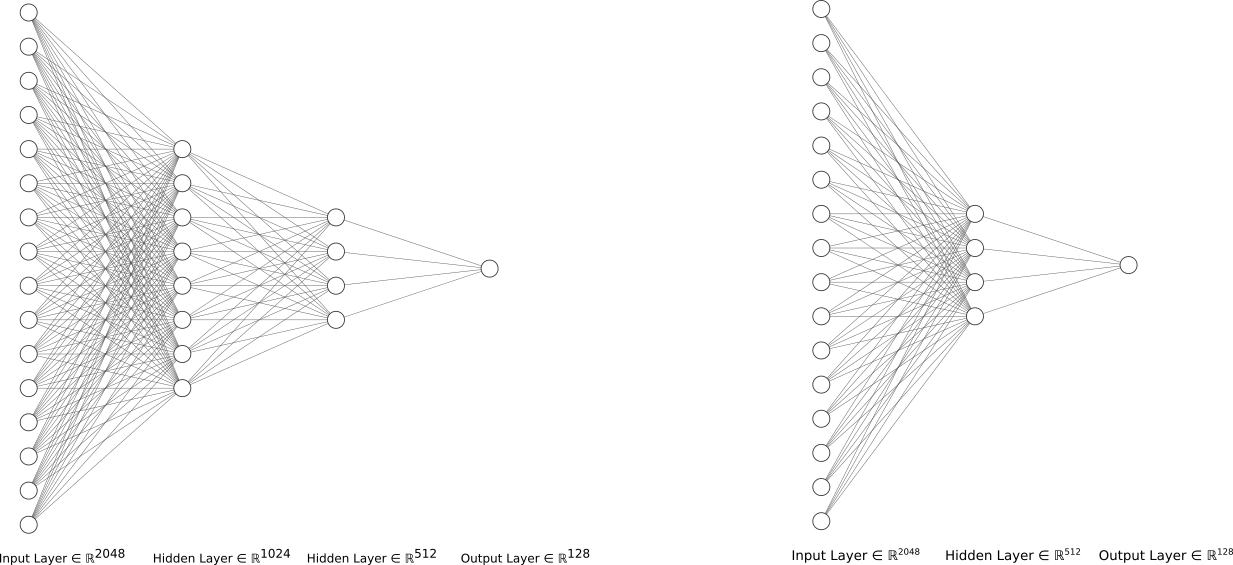
\includegraphics[width=0.8\textwidth]{Images/rl_architecture.png}
    \caption{TOBE CHANGED RL Framework Architecture: Actor-Critic Network}
    \label{fig:rlarchitecture}
\end{figure}

The \ac{RL} framework has been implemented using the \textit{Stable Baselines 3} library \cite{raffin_stable-baselines3_2021}. The \ac{RL} framework has been trained for $10$M steps, which given the episodic length, corresponds to $10$ epochs. The INSERT FIGURE below represents the main metrics collected in the training process. In particular the figure shows the mean reward, the mean episode length, the mean episodic reward, the approximated KL divergence and the explained variance.


\section{Evolutionary Algorithm Core}
\label{sec:EvolutionAlgo}


The evolutionary algorithm has been used in the codesign loop to select motor parameters from a set of possible values. The evolutionary algorithm has been implemented using the \textit{DEAP} library CITE.

The motor set of parameters is composed of three main components: motor inertia, motor viscous friction and gear ratio. This choice has been made in order to keep the number of parameters low, in order to reduce the computational cost of the optimization process. The decision process is then repeated for each motor of the robot, which means that the total number of combination are:

\begin{equation}
    H = \binom{n + k - 1}{k} = \binom{23 + 3 - 1}{3} = \frac{25!}{3! 22!} = 2300
\end{equation}

where $n$ is the number of motors and $k$ is the number of parameters for each motor. In order to reduce the computational expense, we decided to focus on four crucial motors of the robot, which are the motors of the legs. This choice has been made because the legs are the main component of the robot that interacts with the environment, and therefore the choice of the motor parameters has a great impact on the performance of the robot. The total number of combinations is then reduced to:

\begin{equation}
    H = \binom{n + k - 1}{k} = \binom{4 + 3 - 1}{3} = \frac{6!}{3! 3!} = 20
\end{equation}

The evolutionary algorithm has been used to select the motor parameters from the set of possible values. The set of possible values for each parameter is shown in the \cref{tab:motorparams}.

\begin{table}[h]
    \centering
    \begin{tabular}{l c c c}
        \toprule
        \textbf{Motor} & \textsc{Inertia} $[k\mathrm{gm}^2]$ & \textsc{Gear Ratio} & \textsc{Viscous Friction} $[\mathrm{N}s\mathrm{rad}^{-1}]$ \\
        \midrule
        \textbf{S}     & $0.0001$                            & $1/100.0$           & $0.1$                                                      \\
        \textbf{M}     & $0.001$                             & $1/100.0$           & $0.15$                                                     \\
        \textbf{L}     & $0.001$                             & $1/160.0$           & $0.2$                                                      \\
        \bottomrule
    \end{tabular}
    \caption{Motor Set Parameters}
    \label{tab:motorparams}
\end{table}


After a preliminary analysis of the problem, the following parameters have been selected:

\begin{table}
    \centering
    \begin{tabular}{ll}
        \toprule
        \textbf{Parameter}    & \textbf{Value} \\
        \midrule
        Population Size       & $100$          \\
        Number of Generations & $100$          \\
        Crossover Probability & $0.5$          \\
        Mutation Probability  & $0.2$          \\
        \bottomrule
    \end{tabular}
    \caption{Evolutionary Algorithm Hyperparameters}
\end{table}

Given the single objective of the optimization problem, the \ac{NSGA}-III algorithm has been selected as the evolutionary algorithm, as it allows to find a set of solutions that are all Pareto optimal.


\section{Humanoid Robots Codesign Loop}
\label{sec:Codesign}

The problem of humanoid robot codesign can be formalized as a reinforcement learning problem, where the agent is the robot, together with a nonlinear optimization of some hardware parameters, in the case discussed in this work this role is played by a evolutionary algorithm.

The first step of the codesign loop involves some inital design choices, which are then used to create the initial population of the evolutionary algorithm. Then the population gets evaluated running in parallel the \ac{RL} framework for each individual of the population. The evaluation process is repeated for a number of generations, after which the best individual is selected and its parameters are used to update the robot design. The process is then repeated until the robot reaches the desired target fitness or when it reaches the maximum number of generations.

For the evaluation, the reward coming from the \ac{RL} training process is used as the fitness function of the evolutionary algorithm. The fitness function is then normalized to the range $[0,1]$ in order to make the optimization more stable.

\chapter{Experiments and Benchmarking}
\label{chp:contrib_ResultsDiscussion}

\section{Modified Forward Dynamics Benchmark}

The introduction of motor dynamics in the context of a recursive forward dynamics algorithm like \ac{ABA}, involves additional computations that are not present in the original algorithm. In this section, we present a benchmark that compares the performance of the modified \ac{ABA} algorithm with the original one, in order to evaluate the impact of the additional computations on the performance of the algorithm. Furthermore, the accuracy of the modified \ac{ABA} algorithm is evaluated by comparing the results with the ones obtained with the modified Inertia-Matrix method.

Regarding the computational performance, the modified \ac{ABA} algorithm is expected to be slower than the original one, due to the additional computations required to compute the motor dynamics. However, from the results reported in ADD REF TO RESULTS, it is possible to see that the modified \ac{ABA} algorithm is comparably fast to the original one, with a difference of less than $1\%$ in the execution time. This is due to the fact that the additional computations required to compute the motor dynamics are negligible compared to the other computations required by the algorithm.

When evaluating the difference between the results obtained with the modified \ac{ABA} algorithm and the modified Inertia-Matrix method, it is possible to see that the difference depends on the motor inertia values. In particular, the difference is larger for the joints with a smaller motor inertia, while it is smaller for the joints with a larger motor inertia.



\section{Robot Codesign Results}

In this section, we present the results of the robot codesign process, which is the main contribution of this work. We start by presenting the results of the \ac{RL} framework, which is used to optimize the control strategy of the system. Then, we present the results of the \ac{RL} framework with the addition of the genetic algorithm.

\subsection{RL Framework}

For the reinforcement learning training, we opted for the use of \textit{Weights {\&} Biases}\footnote{\url{https://wandb.ai}}, a tool that allows for the tracking of the training metrics and the hyperparameters used during the training. In opposition to the most common \textit{Tensorboard}\footnote{\url{https://www.tensorflow.org/tensorboard}} tool, \textit{Weights {\&} Biases} supports online logging, which allows for the real-time monitoring of the training metrics and more extensive logging capabilities.


\subsubsection{Cartpole Swing-Up}

For the cartpole swing-up task, the metrics obtained during the training with \texttt{stable\_baselines3} together with \jaxsim are reported in \cref{fig:cartpoleresults}.

\begin{figure}
    \centering
    \caption{Cartpole RL Training Metrics}
    \label{fig:cartpoleresults}
    \subfloat[Explained Variance]{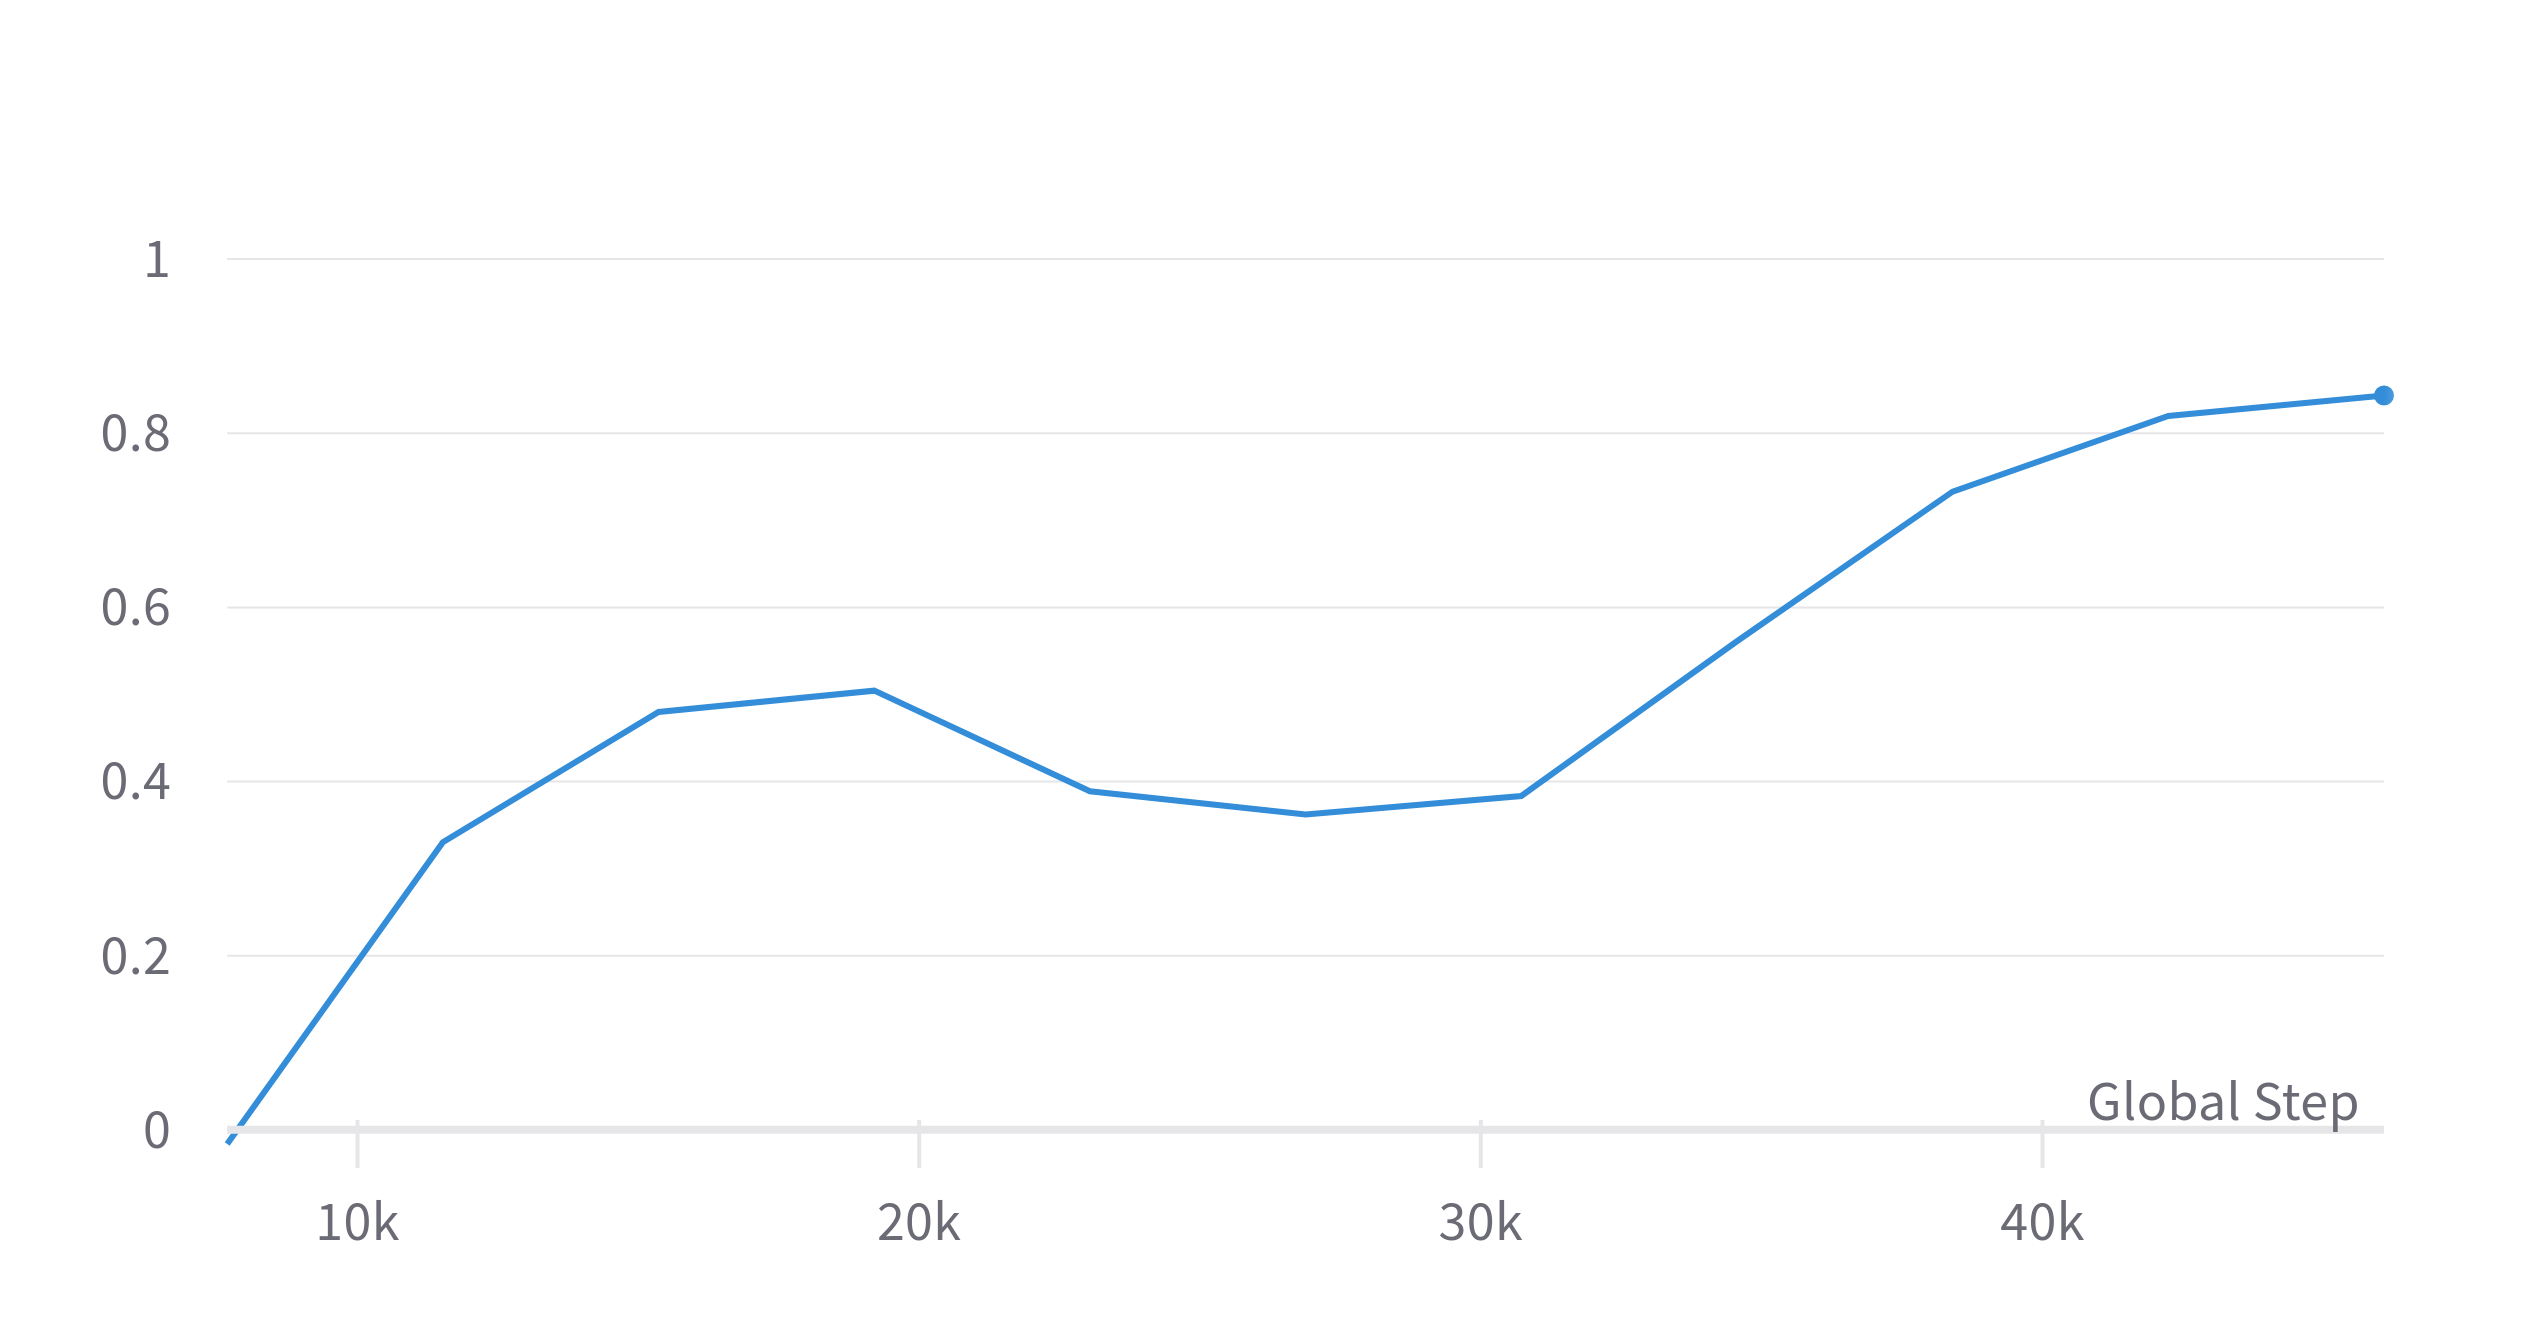
\includegraphics[width=0.45\textwidth]{Images/Results/expvariance_cartpole.png}}
    \subfloat[Approximated KL]{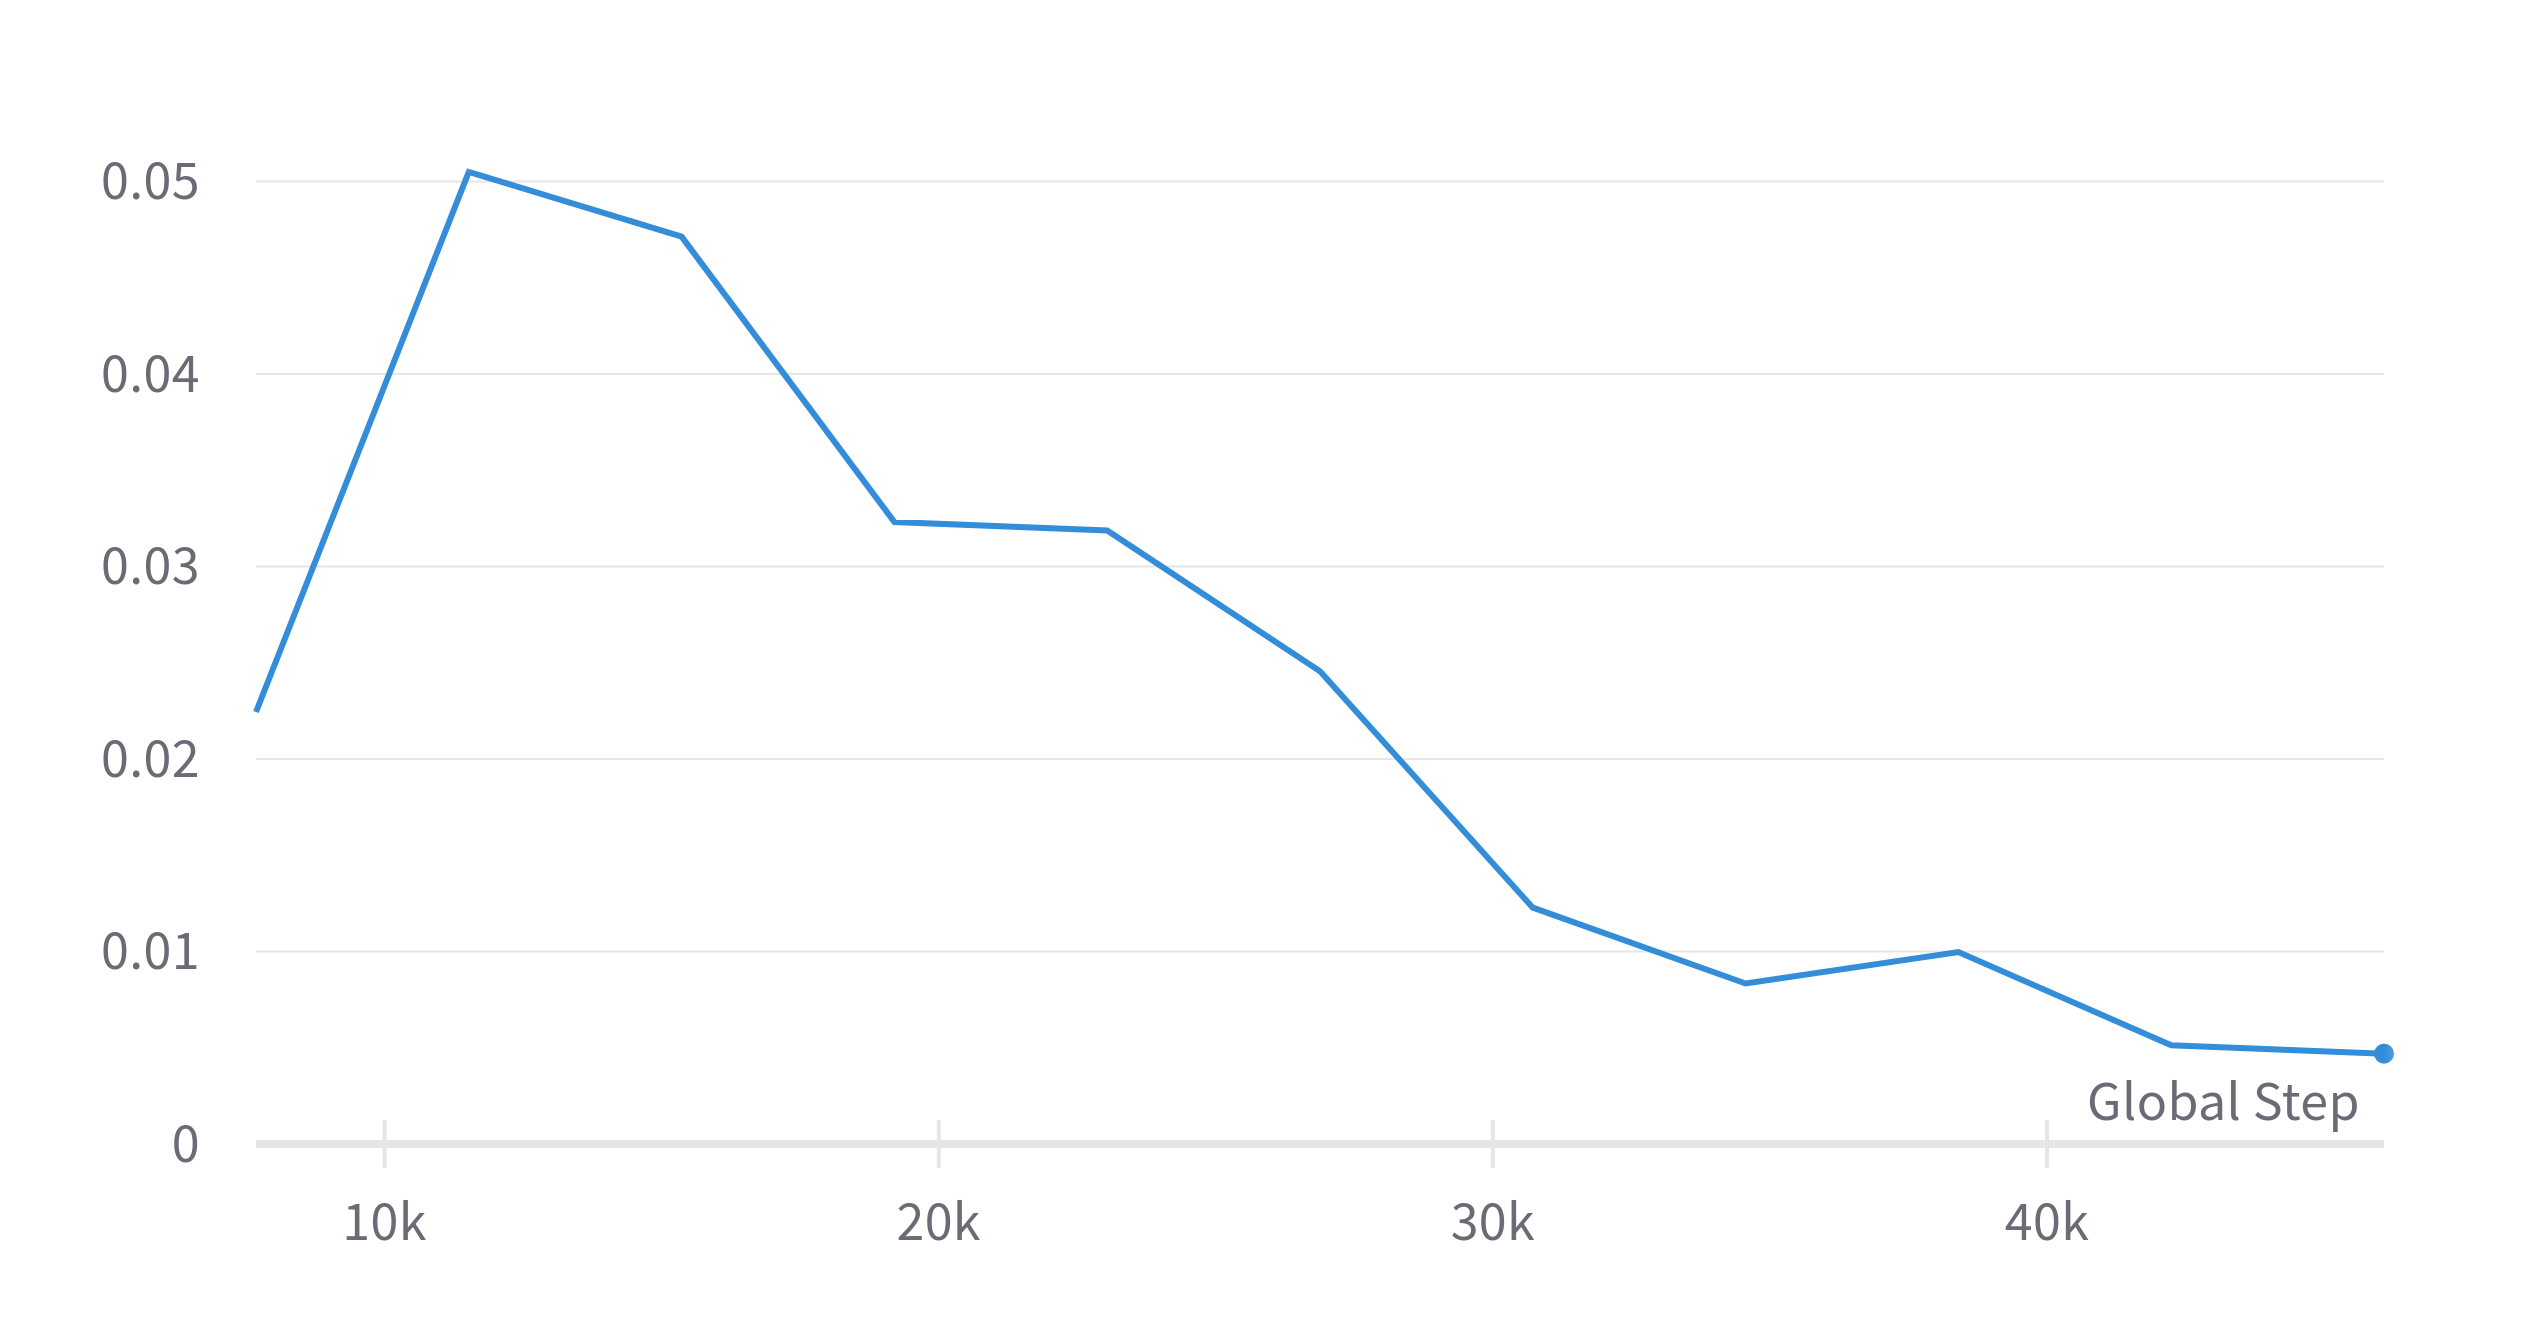
\includegraphics[width=0.45\textwidth]{Images/Results/kl_cartpole.png}} \\
    \subfloat[Value Loss]{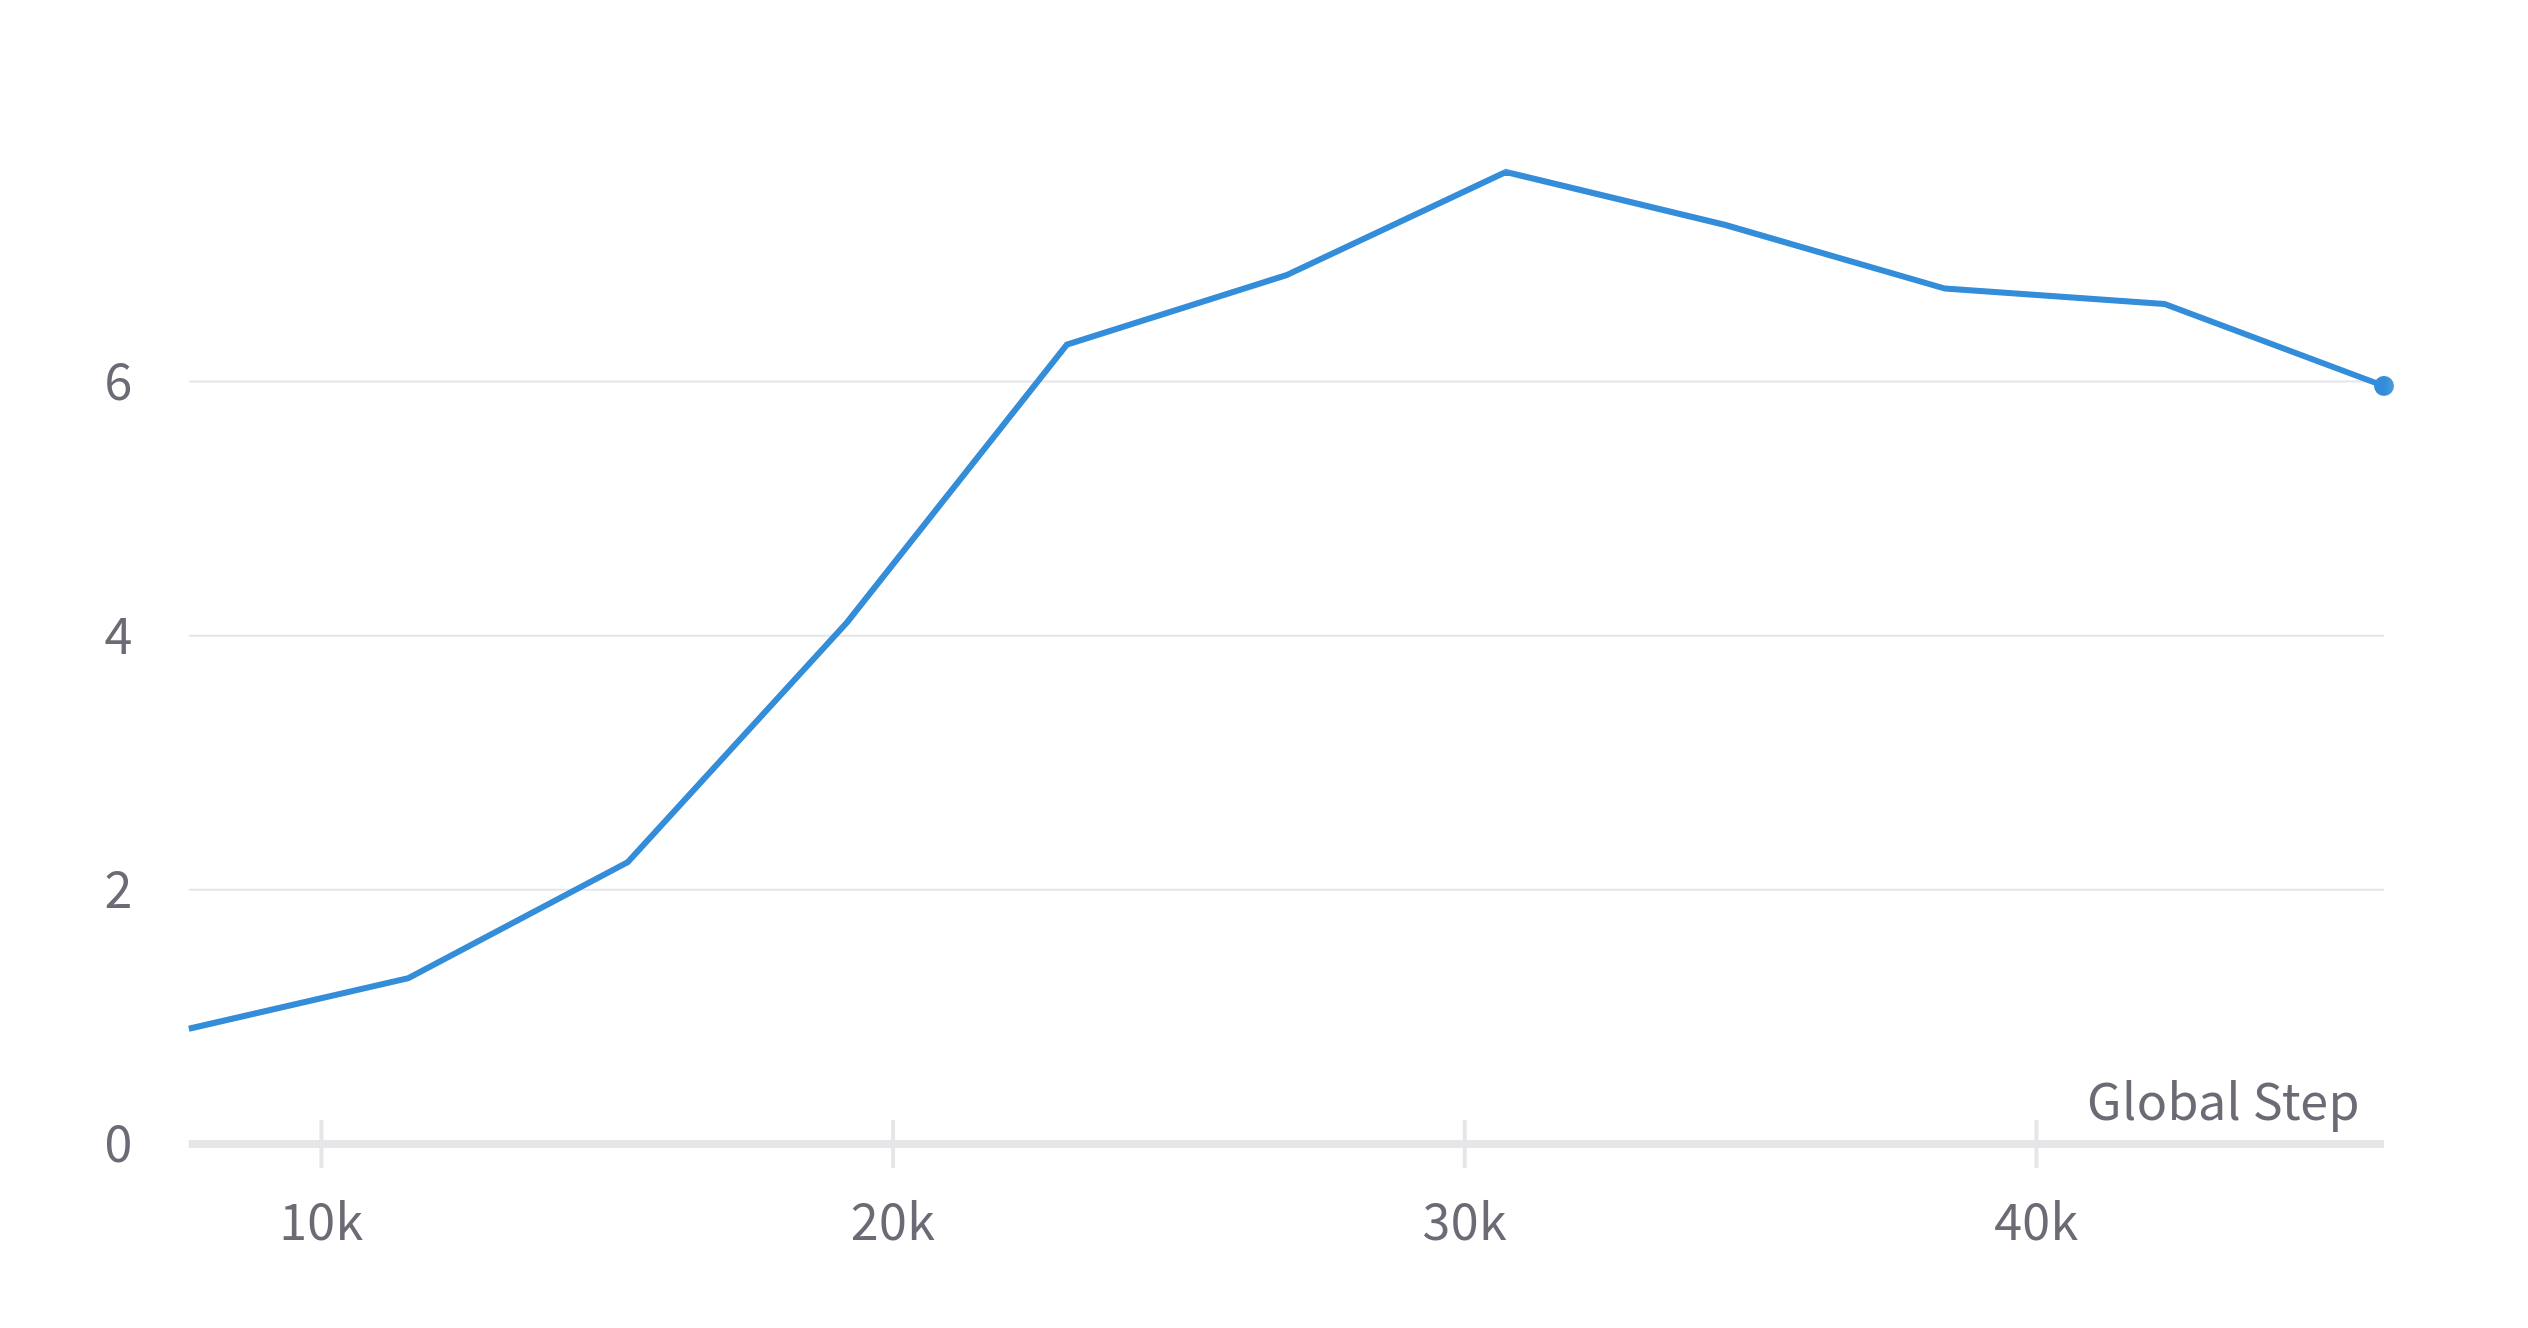
\includegraphics[width=0.45\textwidth]{Images/Results/loss_value_cartpole.png}}
    \subfloat[Rollout Metrics]{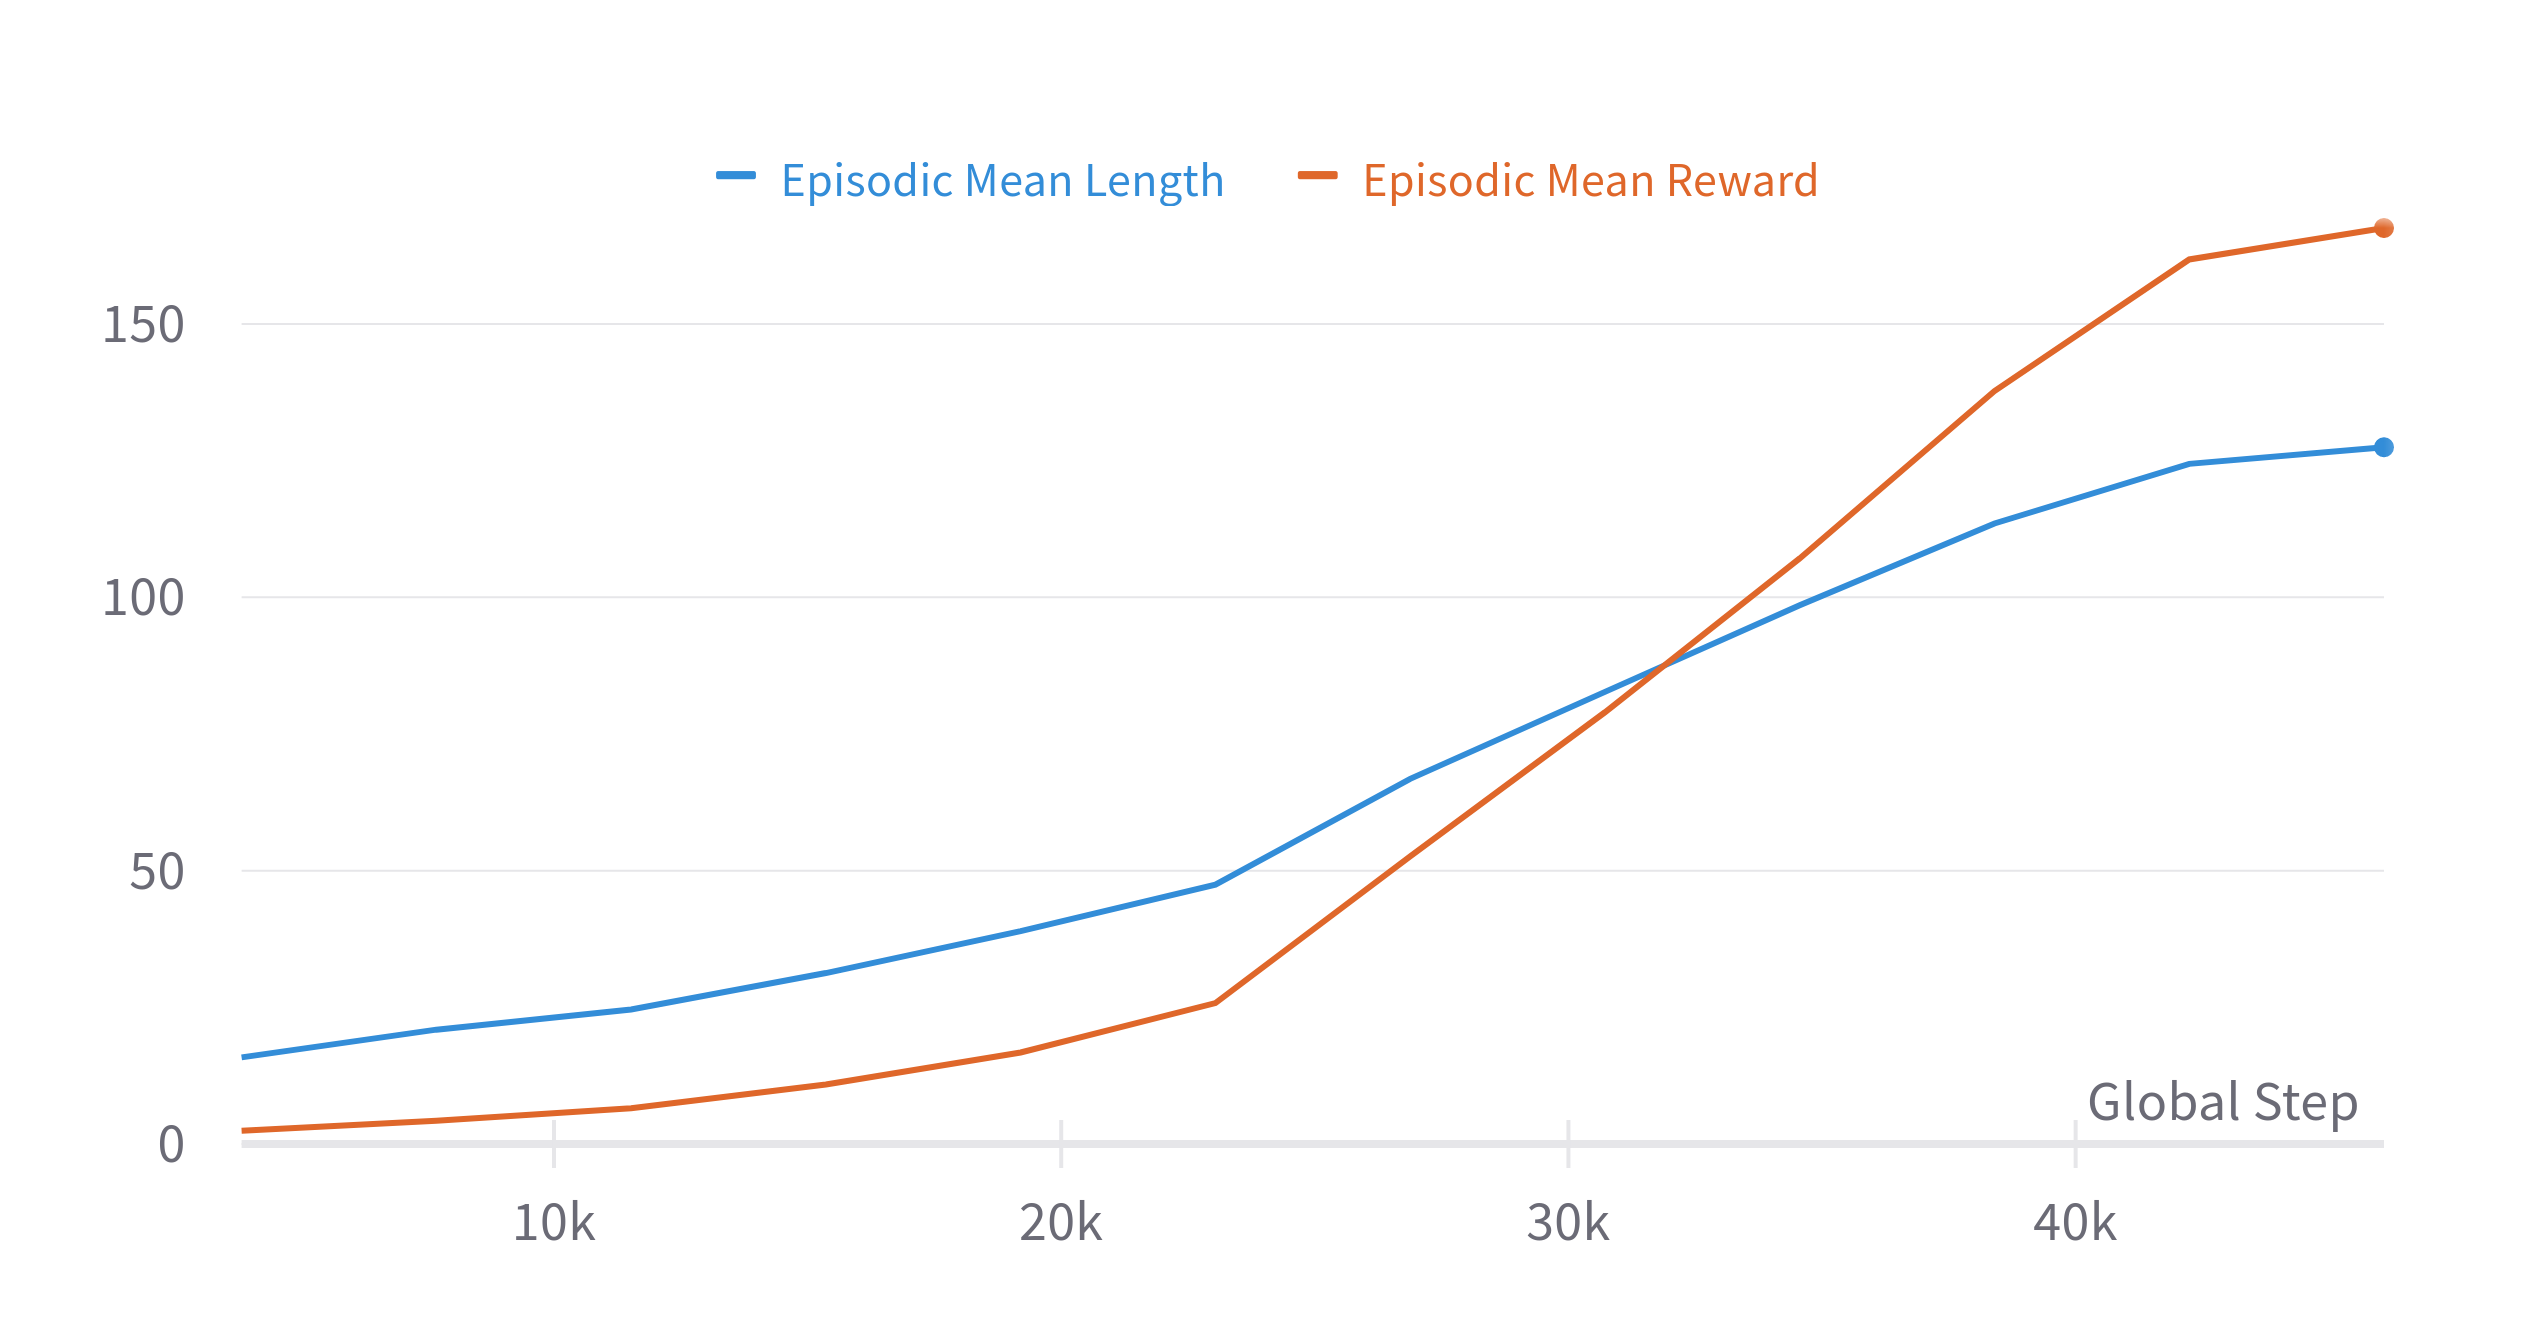
\includegraphics[width=0.45\textwidth]{Images/Results/rollout_cartpole.png}}
\end{figure}

As expected, the explained variance gets closer to $1$ as the training progresses, while the approximated KL divergence remains small, which means that the policy update is not too large. The value loss decreases as the training progresses, which means that the value function is getting better at predicting the return. The rollout metrics show that the mean reward and the mean episode length increase as the training progresses, which means that the policy is getting better at solving the task.

\subsubsection{Stickbot Locomotion}

In \cref{fig:stickbotresults}, the metrics obtained during the training with \textsc{Isaac gym} are reported.

\begin{figure}[h]
    \centering
    \caption{Stickbot RL Training Metrics.}
    \label{fig:stickbotresults}
    \subfloat[Episodic Mean Length]{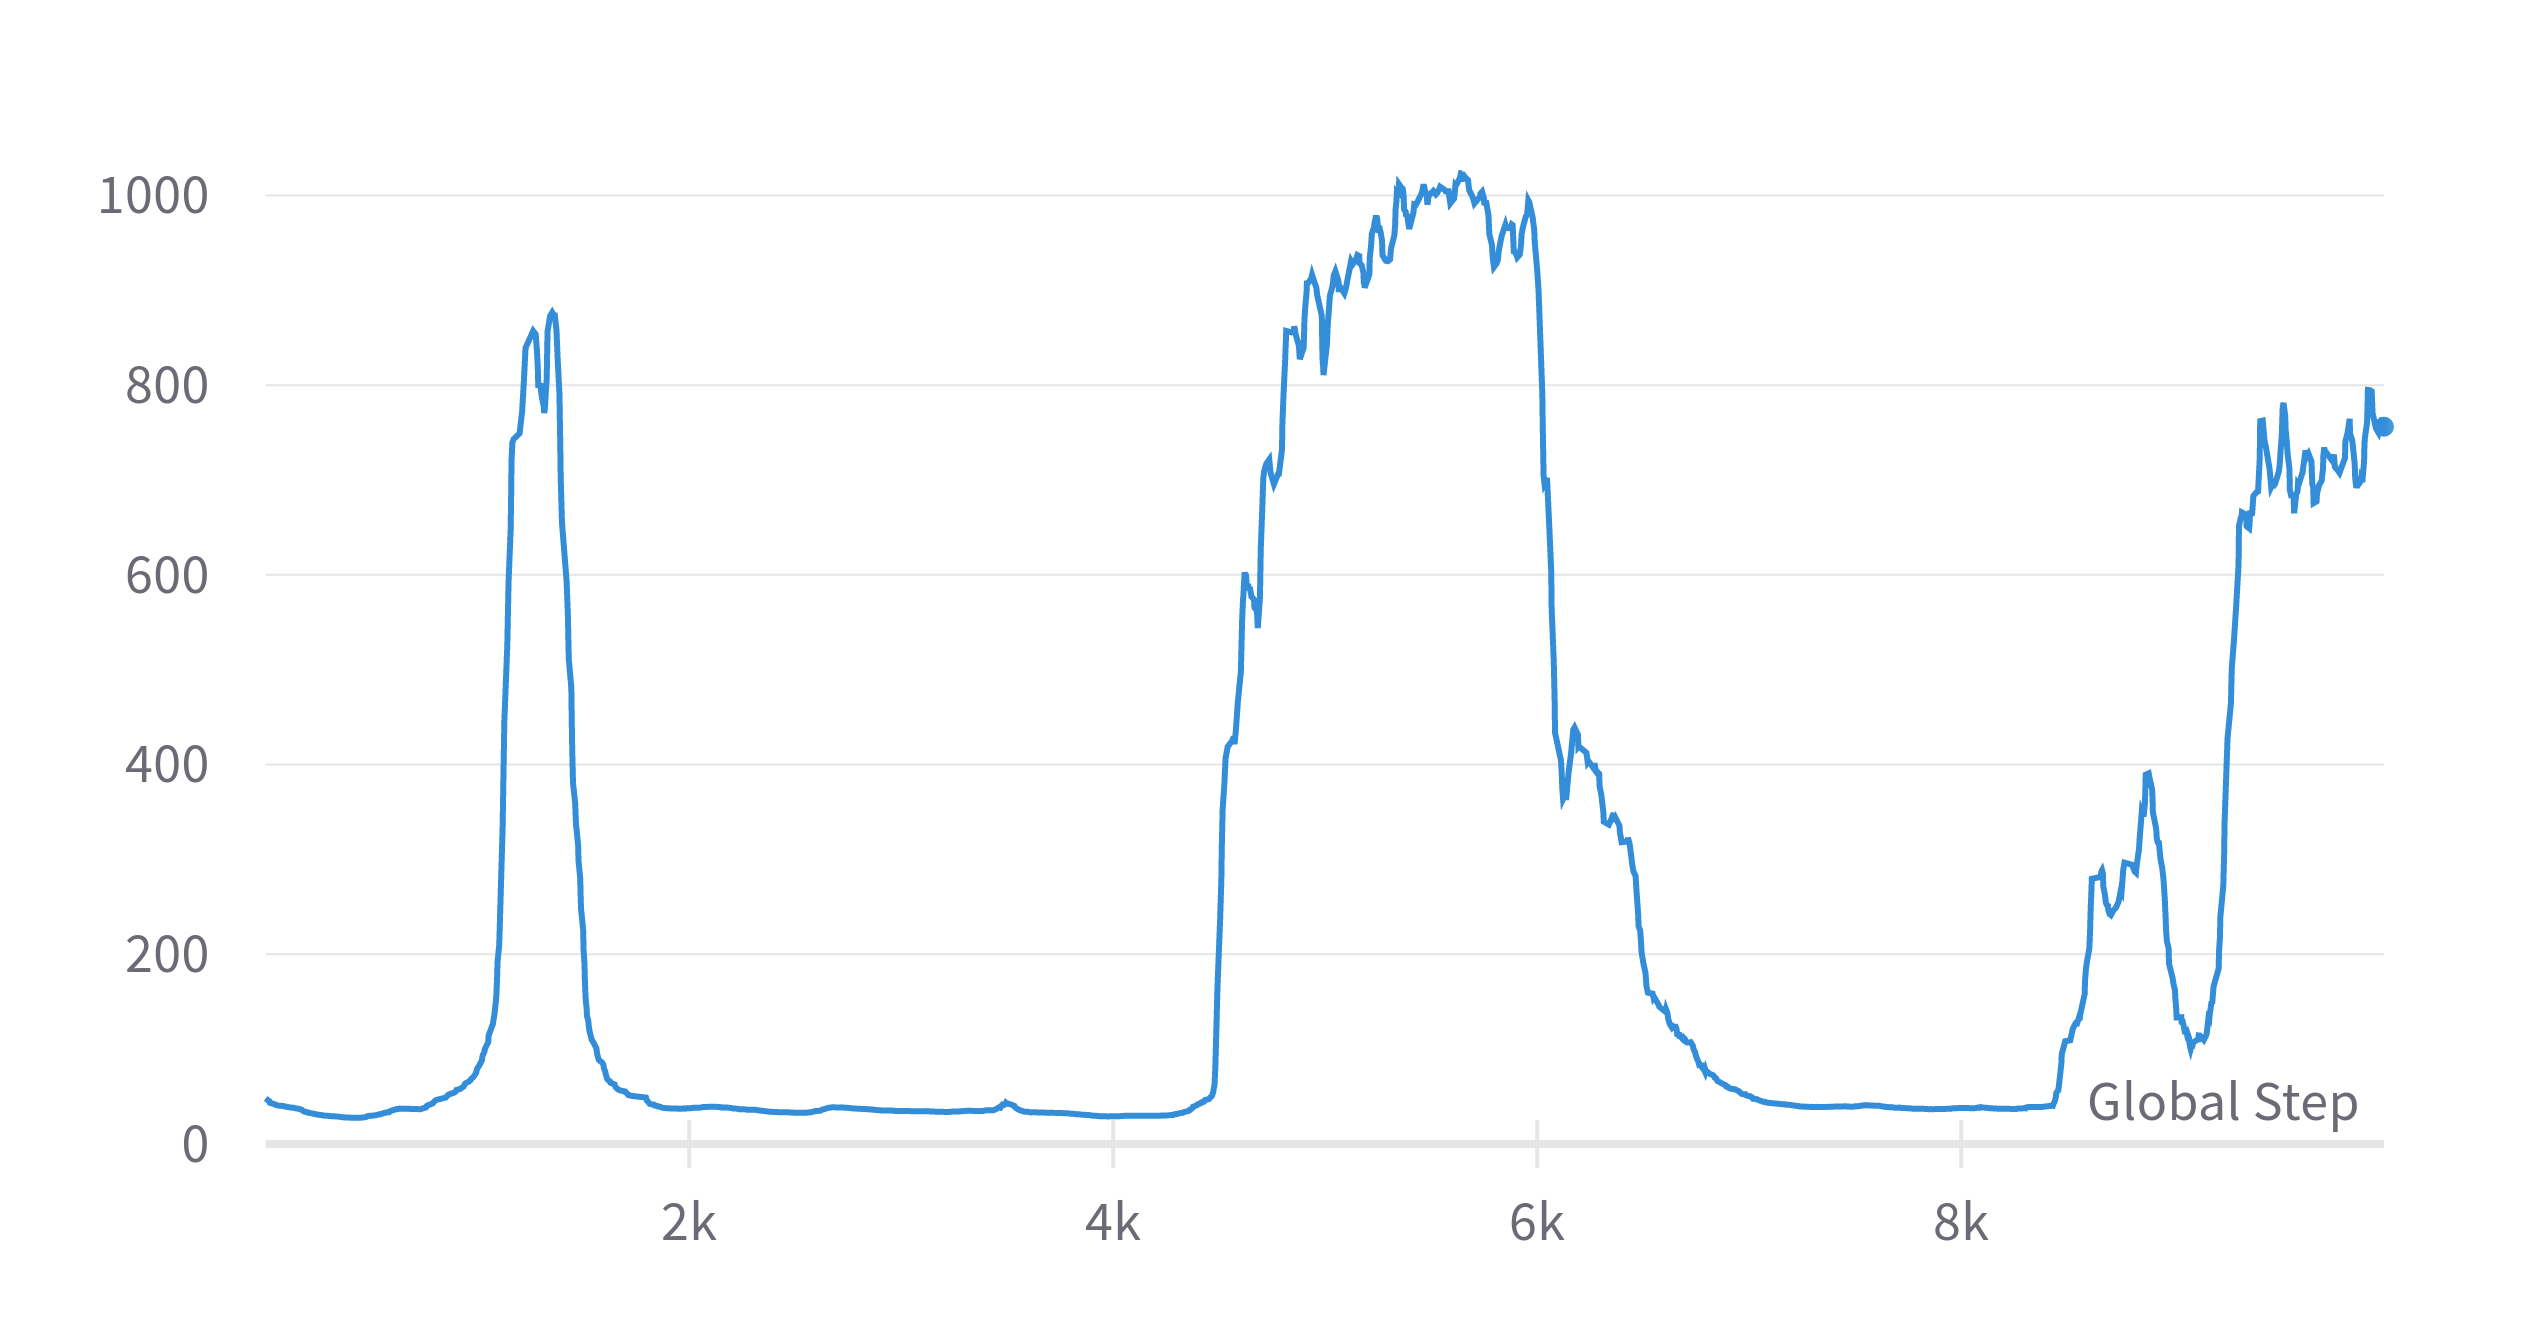
\includegraphics[width=0.45\textwidth]{Images/Results/rollout_eplen_stickbot.png}}
    \subfloat[Episodic Mean Reward]{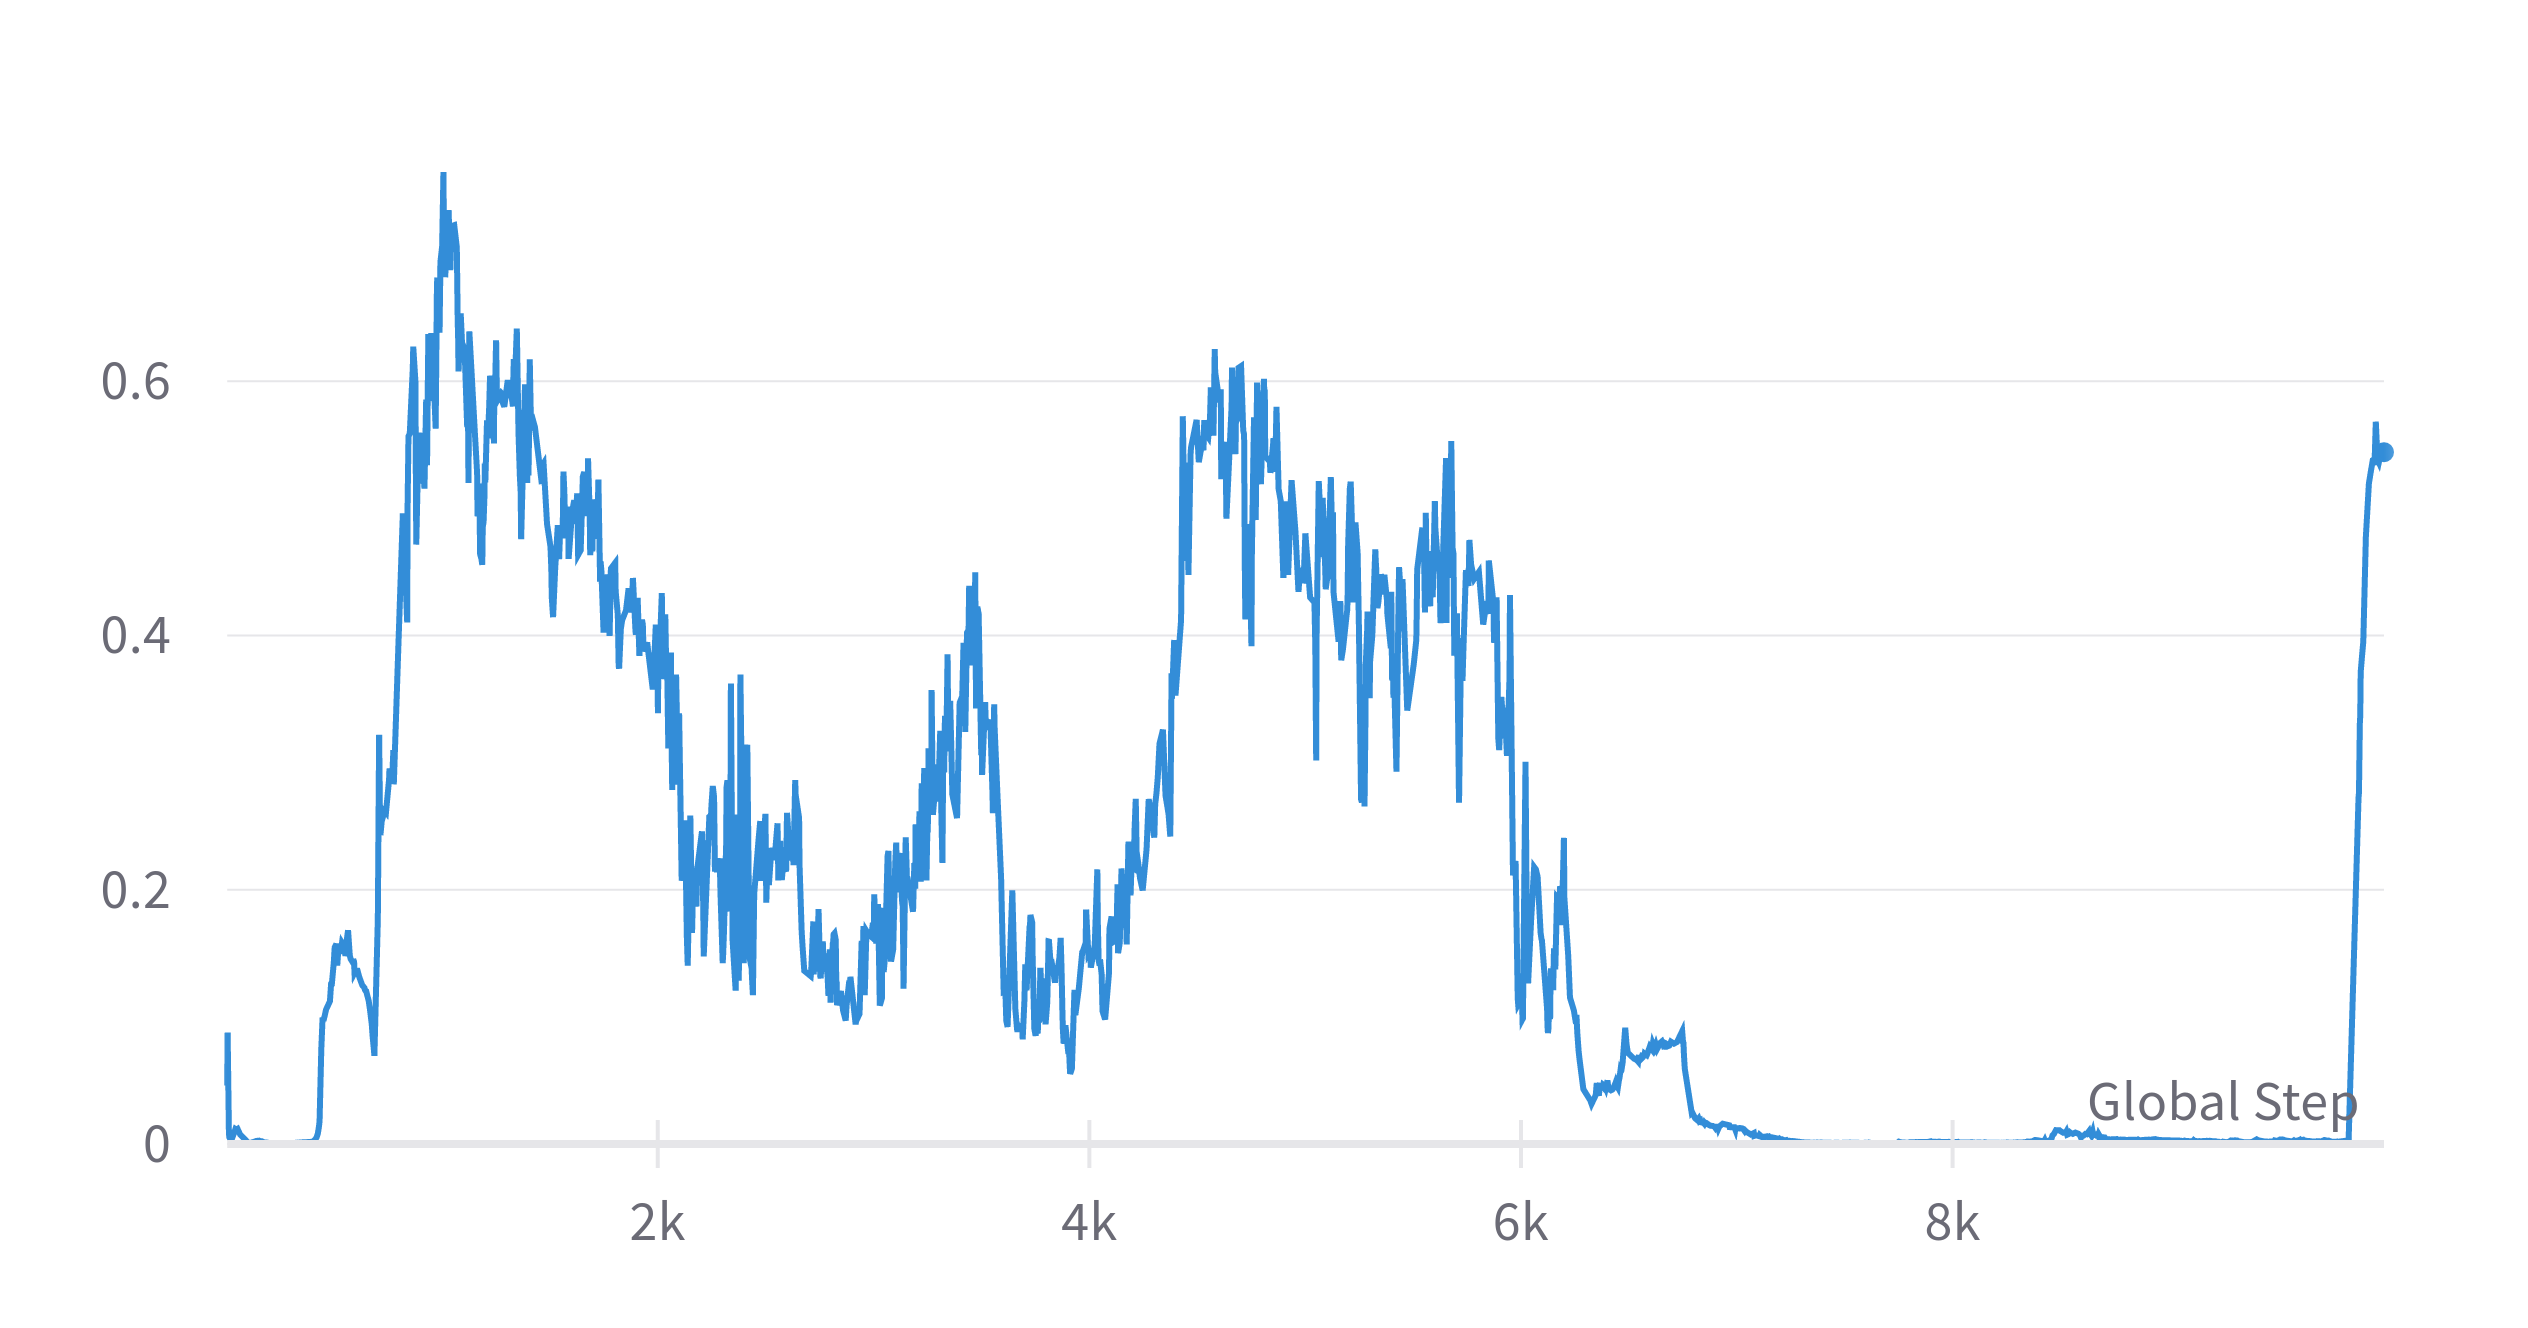
\includegraphics[width=0.45\textwidth]{Images/Results/rollout_meanrew_stickbot.png}}
\end{figure}

The mean episode length and the mean reward increase as the training progresses, which means that the policy is effectively learning to solve the task maximizing the reward.

\subsection{Codesign with Genetic Algorithm}

\begin{figure}[h]
    \centering
    \caption{Cartpole Codesign Results.}
    \subfloat[Fitness Plot \label{fig:fitness}]{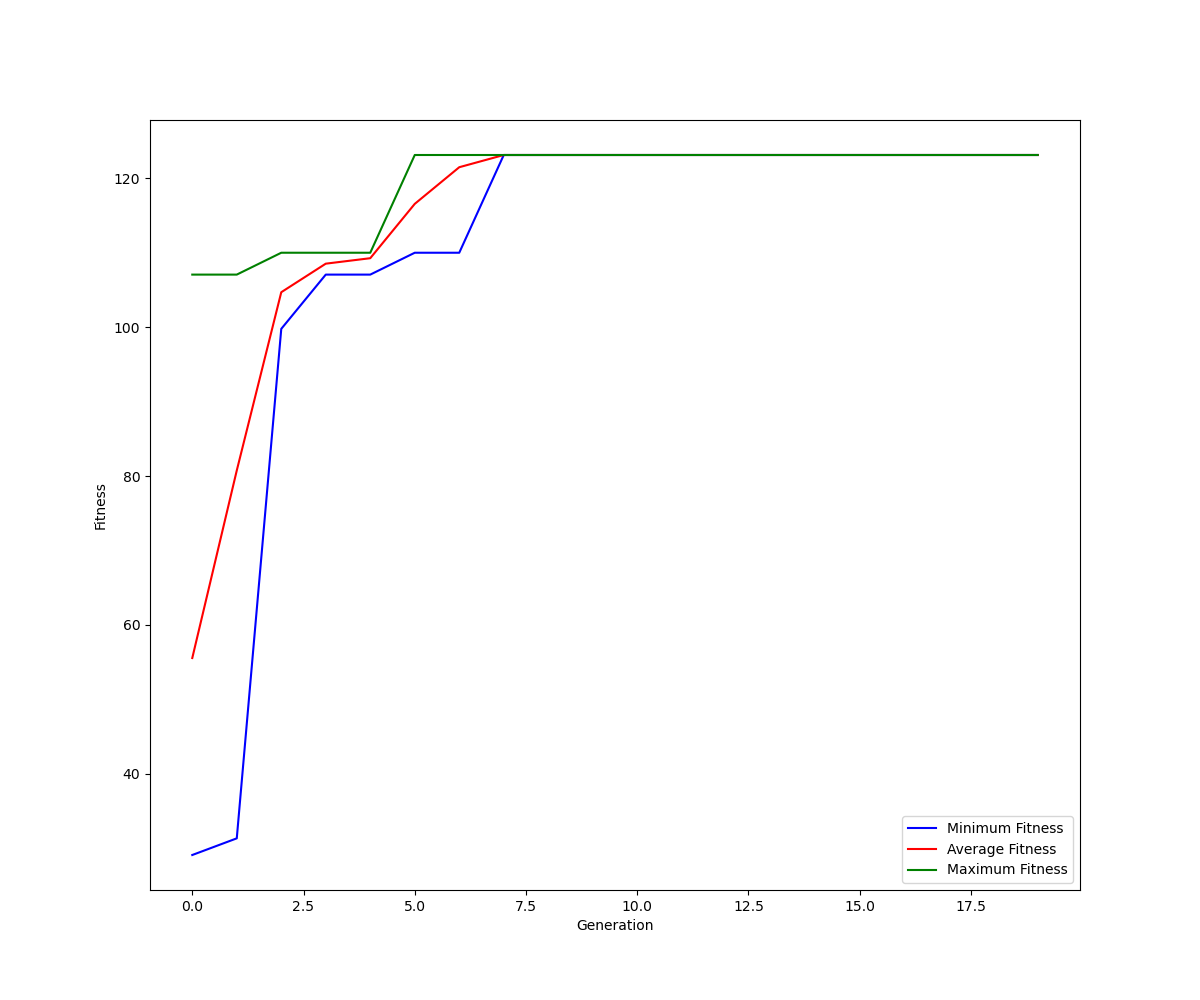
\includegraphics[width=0.4\textwidth]{Images/convergence_plot.png}}
    \subfloat[Diversity Plot \label{fig:diversity}]{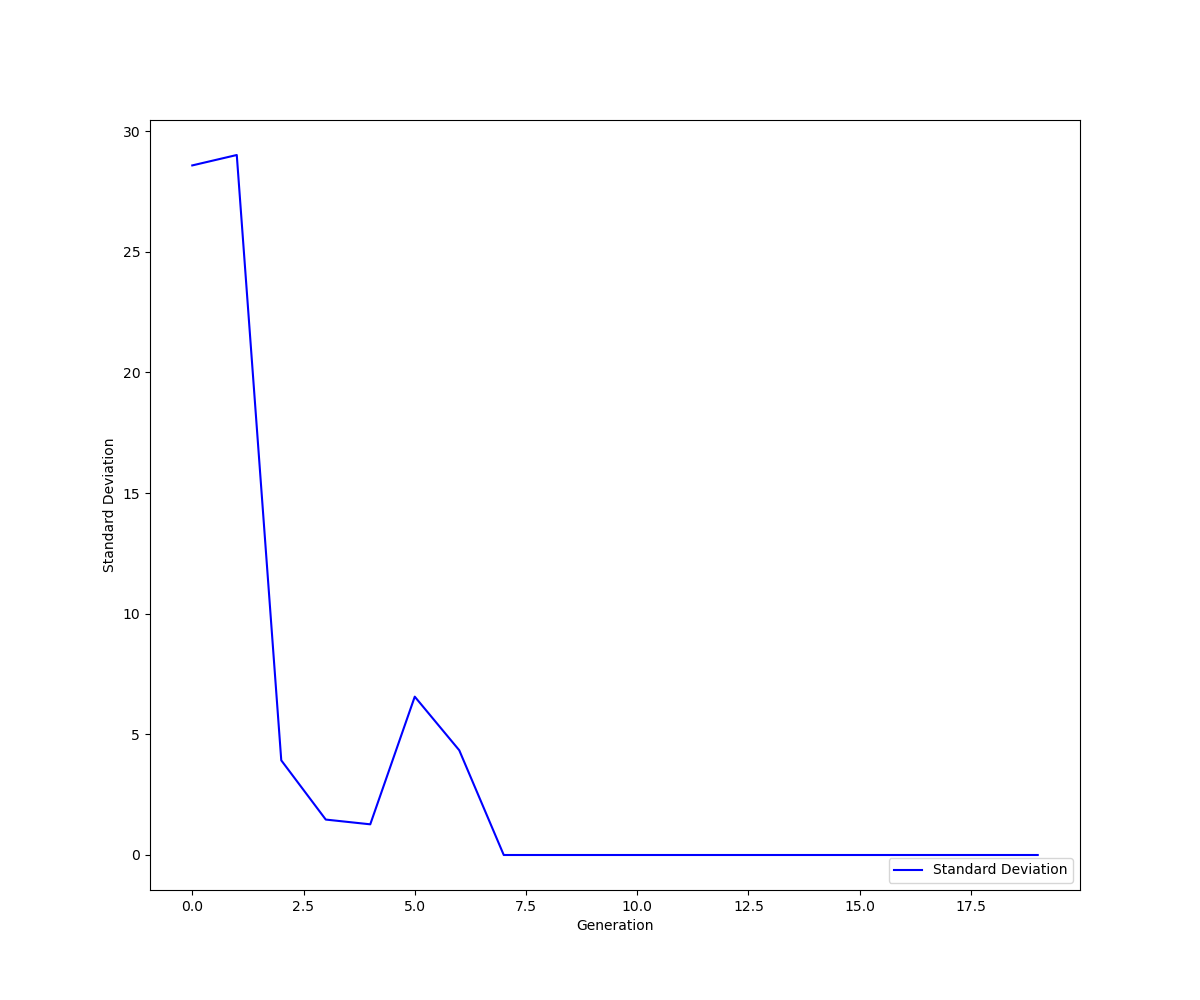
\includegraphics[width=0.4\textwidth]{Images/diversity_plot.png}}
\end{figure}

In this section, we present the results obtained with the genetic algorithm. In particular, we present the results obtained with the codesign
framework for the \textit{Cartpole}.

\begin{figure}
    \centering
    \caption{Evolutionary Algorithm Explored Search Space.}
    \label{fig:searchspace}
    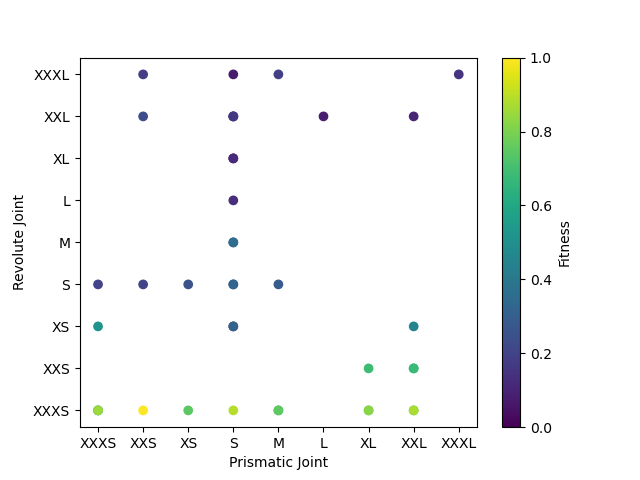
\includegraphics[width=0.5\textwidth]{Images/search_space.png}
\end{figure}

As we can see from \cref{fig:fitness}, the convergence is achieved after SOME generations, with a fitness value of SOME. The diversity decreases as expected, as the population converges to the optimal solution, as we can see from \cref{fig:diversity}.
\chapter{Conclusions and Future Work}
\label{chp:contrib_Conclusions}

The process of implementing a codesign loop has required several intermediate steps. First, the review and adaptation of an already established recursive algorithm for the forward dynamics computation, which allowed to study the effect of the motor dynamics in robotics simulations, then the application of deep reinforcement learning to two main problems, a simple balancing task with a cartpole system, which required the development of an interface between a hardware accelerated simulator like \jaxsim and a reinforcement learning baseline implementation, and a more complex task of locomotion with a humanoid robot, which will represent the major challenge for the future development of the framework. Finally, the implementation of an evolutionary algorithm capable of exploiting synthetic data generated in the reinforcement learning framework in order to optimize the motor parameters of a robot, which allowed to study the effects of the motor design on the robot's performance.

The modified \ac{ABA} algorithm allows for a more realistic forward dynamics computation when there is the need to take into account the motor dynamics while keeping the same computational complexity $\mathcal{O}^n$, making it suitable for real-time applications. However, some hypotheses are still made in the derivation of the algorithm. In particular, future versions of the algorithm might take into account the effect of a non-negligible transmission inertia and the effect of Coulomb friction, which is not considered in the current implementation. Furthermore, eliminating the assumption of equal motion subspace for the motor and the link would allow for the computation of more complex kinematic chains involving, for example, internal kinematic loops or additional degrees of freedom.

The outcomes derived from the reinforcement learning framework demonstrate the efficacy of the suggested approach in solving the tasks considered in this work. However, future versions of \jaxsim might include a more effective and accurate contact model, perhaps exploiting the differentiability of \jax, which has not been extensively studied yet. Moreover, the addition of a more accurate contact model and the development of an integrated visualizer would ease its use as a reinforcement learning playground in combination with the emerging differentiable physics engines.
The framework of \jax could be also exploited to have an open-source version of Adversarial Motion Prior, which exploits the differentiability to easily adapt learned policies to new robots. This would allow for a more effective transfer of learned experience between different robots, which is a crucial aspect in the development of robotic systems.

Finally, the results obtained with the robot codesign process show that the proposed approach is effective in finding a motor combination that is able to maximize the reward. However, the results obtained with the genetic algorithm are limited to a discrete motor parameter set. In the future, supposing to have an unlimited choice for motor design, the codesign loop might take into account continuous search spaces for the motor parameters, which would allow for more in-depth optimization. Moreover, the codesign loop might be extended not only to include the design of the robot morphology parameters, such as the link lengths and density, enabling the algorithm to find the optimal robot design for a given task also from a geometrical point of view, but also to exploit multiple objectives in the optimization process in order to find a trade-off between different aspects of the robot design, such as the energy consumption and the robustness of the robot to external perturbations via the use of a multi-objective genetic algorithm like \ac{NSGA}-III.

\chapter*{Epilogue}
\label{chp:99-Epilogue}

This work presented a novel framework based on the combination of reinforcement learning and evolutionary algorithms for the codesign of humanoid robots supported by hardware accelerated simulators. In particular, it answers the research question:

\begin{quote}
    \textit{
        Can humanoid robots be endowed with embodied cognition?}
\end{quote}

in which \textit{embodied cognition} refers to a synergy between the robot's hardware and the control system that makes an intelligence behavior emerge. In the scope of this thesis, the hardware is represented by the motors actuating the joints of the robot, and the control system is represented by a control policy obtained via deep reinforcement learning.
In order to answer this question, the work presents a novel framework that combines reinforcement learning and evolutionary algorithms to optimize the motor parameters of a robot with respect to a given task. In particular,

\begin{description}
    \item[In \cref{part:background}] the work presented the background knowledge required to understand the work, starting from the notation and the mathematical preliminaries of rigid multibody dynamics. The groundwork was then used to present the original formulation of the \ac{ABA} algorithm, which is the basis for the forward dynamics computation in this framework. Then, we moved to an overview of the current state of the art in the scope of hardware accelerated simulators, with a focus on the emerging role of \jax in the field of deep learning and robotics. Finally, the theoretical background of deep reinforcement learning and evolutionary algorithms was presented, introducing the reader to the main concepts of the two fields and the most common algorithms used in the literature.
    \item[In \cref{part:contributions}] the thesis proposed the two main contribution of the thesis. First, it guided the reader to the understanding of the implementation of a modified version of the \ac{ABA} algorithm that allows a holistic computation of the forward dynamics of a multibody system when there is the need to take into account the motor dynamics. Moreover, the reformulation served as an additional feature for the hardware accelerated \jaxsim simulator, allowing to consider the effect of rotors in the robot joints during simulation. As a second contribution, the thesis described the implementation of a codesign loop which creates a synergy between reinforcement learning and evolutionary algorithms in order to guide the optimization of the motor parameters of a robot, while learning a policy able to act as its control system.
\end{description}

This work addressed therefore the problem of the limited offer of simulation environments that allow for a computation of the forward dynamics that takes into account the presence of motors mounted on the joints of the robot in a hardware accelerated simulator. The framework was tested on a simple, yet easily scalable environment, and the results showed that the developed architecture is able to find a set of motor parameters that allows for a better reward in the reinforcement learning scenario.
The proposed approach for the codesign can potentially be a starting point for a further extension to the generation of new humanoid robots in which the hardware is optimized together with the control strategy. Furthermore, it could be propelled by the recent advances in the field of hardware acceleration and the development of differentiable physics engines, which is crucial for the development of a more extensive co-optimization architecture.

%-------------------------------------------------------------------------
%	BIBLIOGRAPHY
%-------------------------------------------------------------------------

\addtocontents{toc}{\vspace{2em}} % Add a gap in the Contents, for aesthetics
\bibliography{references}

%-------------------------------------------------------------------------
%	APPENDICES
%-------------------------------------------------------------------------

\cleardoublepage
\addtocontents{toc}{\vspace{2em}} % Add a gap in the Contents, for aesthetics
\appendix
\chapter{Appendix A}
If you need to include an appendix to support the research in your thesis, you can place it at the end of the manuscript.
An appendix contains supplementary material (figures, tables, data, codes, mathematical proofs, surveys, \dots)
which supplement the main results contained in the previous chapters.

\chapter{Appendix B}
It may be necessary to include another appendix to better organize the presentation of supplementary material.


% LIST OF FIGURES
\listoffigures

% LIST OF TABLES
\listoftables

% LIST OF SYMBOLS
% Write out the List of Symbols in this page
% \chapter*{List of Symbols} % You have to include a chapter for your list of symbols (
% \begin{table}[H]
%     \centering
%     \begin{tabular}{lll}
%         \textbf{Variable} & \textbf{Description} & \textbf{SI unit} \\\hline\\[-9px]
%         $\bm{u}$ & solid displacement & m \\[2px]
%         $\bm{u}_f$ & fluid displacement & m \\[2px]
%     \end{tabular}
% \end{table}

% ACKNOWLEDGEMENTS
\chapter*{Acknowledgements}
Here you might want to acknowledge someone.


\cleardoublepage

\end{document}
